 \documentclass[a4paper,BCOR=15mm,bibliography=totoc,headings=optiontohead, cleardoublepage=plain]{scrbook}

\usepackage{fontspec}
\defaultfontfeatures{Ligatures=TeX}
  \setmainfont{Tex Gyre Pagella}
  \setsansfont{Tex Gyre Heros}
  \setmonofont{Latin Modern Mono}

\setkomafont{caption}{\small}

\usepackage{scrlayer-scrpage}
  \pagestyle{scrheadings}
  \renewcommand*{\figureformat}{Fig.~\thefigure\autodot}
  \renewcommand*{\tableformat}{Tab.~\thetable\autodot}


\usepackage{csquotes}
\usepackage{polyglossia}
\setdefaultlanguage{english}
\setotherlanguages{german}

\usepackage[style=numeric-comp,sorting=none,backend=biber,giveninits=true,doi=false]{biblatex}
% Define fields for "article' entries"
\DeclareFieldFormat[article]{title}{\emph{#1},}
\DeclareFieldFormat[article]{journaltitle}{#1}
\DeclareFieldFormat[article]{volume}{\textbf{#1}}
\DeclareFieldFormat[article]{pages}{#1}
\DeclareFieldFormat[article]{year}{(#1)\nopunct}
% Define fields for "report' entries"
\DeclareFieldFormat[report]{title}{\emph{#1},}
% Define fields for "book' entries"
\DeclareFieldFormat[book]{title}{\emph{#1},}
\DeclareFieldFormat[book]{edition}{\ifnum#1=1%
                                    \emph{#1st ed\adddot}
                                   \else \ifnum#1=2%
                                           \emph{#1nd ed\adddot}
                                         \else \ifnum#1=3%
                                                 \emph{#1rd ed\adddot}
                                               \else \emph{#1th ed\adddot} \fi \fi \fi}

\DefineBibliographyStrings{english}{andothers = {{et\:al\adddot}},}%et al statt u.a.
\renewcommand*{\newunitpunct}{\addcomma\space}  % Komma statt Punkt als defaulttrennzeichen zwischen Einträgen in Bibliography

% remove comma after date/before 'identifier' of journal - therefore at the moment no comma before pages is visible...TODO
\renewbibmacro{issue+date}{%
  \printtext[parens]{%
    \iffieldundef{issue}
      {\usebibmacro{date}}
      {\printfield{issue}%
       \setunit*{\addspace}%
       \usebibmacro{date}}}%
  \nopunct\newunit}

% skipping the "in" before editing the journal
\renewbibmacro{in:}{}
% proper usage of "collaboration" field in arrticles (therefore also the author bibmacro needs to be redefined below)
\DeclareSourcemap{
 \maps[datatype=bibtex,overwrite=true]{
  \map{
    \step[fieldsource=Collaboration, final=true]
    \step[fieldset=usera, origfieldval, final=true]
  }
 }
}
\renewbibmacro*{author}{%
  \iffieldundef{usera}{%
    \printnames{author}%
  }{%
    \printfield{usera}, \printnames{author}%
  }%
}%
% adding the bibliography file
\addbibresource{miscellaneous.bib}
\addbibresource{detector.bib}
\addbibresource{textbooks.bib}
\addbibresource{theory.bib}
\addbibresource{experiments.bib}

\usepackage{url}
\usepackage{hyperref}
\hypersetup{
    pdfauthor = {Alex Birnkraut, alex.birnkraut@tu-dortmund.de},
    pdftitle = {Measurement of CPV in Bd->Dpi},
    pdfsubject = {Time dependent CP violation measurement},
    pdfkeywords = {HEP, CERN, LHC, LHCb, CP violation, b physics, flavour physics},
    pdfcreator = {LaTeX with hyperref package},
    pdfproducer = {lualatex}
    }
\usepackage{slashed}

\usepackage{microtype}

\usepackage{mathtools}
\usepackage[bold-style=ISO, math-style=ISO]{unicode-math}
\setmathfont{Tex Gyre Pagella Math}

\usepackage[locale=UK,input-ignore={.},separate-uncertainty=true]{siunitx}
\DeclareSIUnit{\clight}{c}
\DeclareSIUnit{\MeVc}{\mega\electronvolt\per\clight}
\DeclareSIUnit{\GeVc}{\giga\electronvolt\per\clight}
\DeclareSIUnit{\MeVcc}{\mega\electronvolt\per\clight\squared}
\DeclareSIUnit{\GeVcc}{\giga\electronvolt\per\clight\squared}
\usepackage{xfrac}
\usepackage{nicefrac}

\usepackage{cleveref}
\crefname{chapter}{Ch.\@}{Chs.\@}
\crefname{section}{Sec.\@}{Secs.\@}
\crefname{subsection}{Sec.\@}{Secs.\@}
\crefname{figure}{Fig.\@}{Figs.\@}
\crefname{table}{Tab.\@}{Tab.\@}
\crefname{equation}{Eq.\@}{Eqs.\@}

\usepackage{enumerate}

\usepackage{graphicx}

\usepackage{booktabs}
\usepackage{multirow}
\usepackage{tabulary}
\usepackage{threeparttable}

\usepackage{ifthen}
\newboolean{uprightparticles}
\setboolean{uprightparticles}{false} %Set true for upright particle symbols
\usepackage{xspace}
\usepackage{upgreek}
%%% $Id: lhcb-symbols-def.tex 56342 2014-06-20 08:48:41Z roldeman $
%%% ======================================================================
%%% Purpose: Standard LHCb aliases
%%% Author: Originally Ulrik Egede, adapted by Tomasz Skwarnicki for templates,
%%% rewritten by Chris Parkes
%%% Maintainer : Ulrik Egede (2010 - 2012)
%%% Maintainer : Rolf Oldeman (2012 - 2014)
%%% =======================================================================

%%% To use this file outside the normal LHCb document environment, the
%%% following should be added in a preamble (before \begin{document}
%%%
%%%\usepackage{ifthen}
%%%\newboolean{uprightparticles}
%%%\setboolean{uprightparticles}{false} %Set true for upright particle symbols
%%% \usepackage{xspace}
%%% \usepackage{upgreek}

%%%%%%%%%%%%%%%%%%%%%%%%%%%%%%%%%%%%%%%%%%%%%%%%%%%%%%%%%%%%
%%%
%%% The following is to ensure that the template automatically can process
%%% this file.
%%%
%%% Add comments with at least three %%% preceding.
%%% Add new sections with one % preceding
%%% Add new subsections with two %% preceding
%%%%%%%%%%%%%%%%%%%%%%%%%%%%%%%%%%%%%%%%%%%%%%%%%%%%%%%%%%%%

%%%%%%%%%%%%%
% Experiments
%%%%%%%%%%%%%
\def\lhcb {\mbox{LHCb}\xspace}
\def\atlas  {\mbox{ATLAS}\xspace}
\def\cms    {\mbox{CMS}\xspace}
\def\alice  {\mbox{ALICE}\xspace}
\def\babar  {\mbox{BaBar}\xspace}
\def\belle  {\mbox{Belle}\xspace}
\def\cleo   {\mbox{CLEO}\xspace}
\def\cdf    {\mbox{CDF}\xspace}
\def\dzero  {\mbox{D0}\xspace}
\def\aleph  {\mbox{ALEPH}\xspace}
\def\delphi {\mbox{DELPHI}\xspace}
\def\opal   {\mbox{OPAL}\xspace}
\def\lthree {\mbox{L3}\xspace}
\def\sld    {\mbox{SLD}\xspace}
%%%\def\argus  {\mbox{ARGUS}\xspace}
%%%\def\uaone  {\mbox{UA1}\xspace}
%%%\def\uatwo  {\mbox{UA2}\xspace}
%%%\def\ux85 {\mbox{UX85}\xspace}
\def\cern {\mbox{CERN}\xspace}
\def\lhc    {\mbox{LHC}\xspace}
\def\lep    {\mbox{LEP}\xspace}
\def\tevatron {Tevatron\xspace}

%% LHCb sub-detectors and sub-systems

%%%\def\pu     {PU\xspace}
\def\velo   {VELO\xspace}
\def\rich   {RICH\xspace}
\def\richone {RICH1\xspace}
\def\richtwo {RICH2\xspace}
\def\ttracker {TT\xspace}
\def\intr   {IT\xspace}
\def\st     {ST\xspace}
\def\ot     {OT\xspace}
%%%\def\Tone   {T1\xspace}
%%%\def\Ttwo   {T2\xspace}
%%%\def\Tthree {T3\xspace}
%%%\def\Mone   {M1\xspace}
%%%\def\Mtwo   {M2\xspace}
%%%\def\Mthree {M3\xspace}
%%%\def\Mfour  {M4\xspace}
%%%\def\Mfive  {M5\xspace}
\def\spd    {SPD\xspace}
\def\presh  {PS\xspace}
\def\ecal   {ECAL\xspace}
\def\hcal   {HCAL\xspace}
%%%\def\bcm    {BCM\xspace}
\def\MagUp {\mbox{\em Mag\kern -0.05em Up}\xspace}
\def\MagDown {\mbox{\em MagDown}\xspace}

%%%\def\ode    {ODE\xspace}
%%%\def\daq    {DAQ\xspace}
%%%\def\tfc    {TFC\xspace}
%%%\def\ecs    {ECS\xspace}
%%%\def\lone   {L0\xspace}
%%%\def\hlt    {HLT\xspace}
%%%\def\hltone {HLT1\xspace}
%%%\def\hlttwo {HLT2\xspace}

%%% Upright (not slanted) Particles

\ifthenelse{\boolean{uprightparticles}}%
{\def\Palpha      {\ensuremath{\upalpha}\xspace}
 \def\Pbeta       {\ensuremath{\upbeta}\xspace}
 \def\Pgamma      {\ensuremath{\upgamma}\xspace}
 \def\Pdelta      {\ensuremath{\updelta}\xspace}
 \def\Pepsilon    {\ensuremath{\upepsilon}\xspace}
 \def\Pvarepsilon {\ensuremath{\upvarepsilon}\xspace}
 \def\Pzeta       {\ensuremath{\upzeta}\xspace}
 \def\Peta        {\ensuremath{\upeta}\xspace}
 \def\Ptheta      {\ensuremath{\uptheta}\xspace}
 \def\Pvartheta   {\ensuremath{\upvartheta}\xspace}
 \def\Piota       {\ensuremath{\upiota}\xspace}
 \def\Pkappa      {\ensuremath{\upkappa}\xspace}
 \def\Plambda     {\ensuremath{\uplambda}\xspace}
 \def\Pmu         {\ensuremath{\upmu}\xspace}
 \def\Pnu         {\ensuremath{\upnu}\xspace}
 \def\Pxi         {\ensuremath{\upxi}\xspace}
 \def\Ppi         {\ensuremath{\uppi}\xspace}
 \def\Pvarpi      {\ensuremath{\upvarpi}\xspace}
 \def\Prho        {\ensuremath{\uprho}\xspace}
 \def\Pvarrho     {\ensuremath{\upvarrho}\xspace}
 \def\Ptau        {\ensuremath{\uptau}\xspace}
 \def\Pupsilon    {\ensuremath{\upupsilon}\xspace}
 \def\Pphi        {\ensuremath{\upphi}\xspace}
 \def\Pvarphi     {\ensuremath{\upvarphi}\xspace}
 \def\Pchi        {\ensuremath{\upchi}\xspace}
 \def\Ppsi        {\ensuremath{\uppsi}\xspace}
 \def\Pomega      {\ensuremath{\upomega}\xspace}

 \def\PDelta      {\ensuremath{\Delta}\xspace}
 \def\PXi      {\ensuremath{\Xi}\xspace}
 \def\PLambda      {\ensuremath{\Lambda}\xspace}
 \def\PSigma      {\ensuremath{\Sigma}\xspace}
 \def\POmega      {\ensuremath{\Omega}\xspace}
 \def\PUpsilon      {\ensuremath{\Upsilon}\xspace}

 %\mathchardef\Deltares="7101
 %\mathchardef\Xi="7104
 %\mathchardef\Lambda="7103
 %\mathchardef\Sigma="7106
 %\mathchardef\Omega="710A


 \def\PA      {\ensuremath{\mathrm{A}}\xspace}
 \def\PB      {\ensuremath{\mathrm{B}}\xspace}
 \def\PC      {\ensuremath{\mathrm{C}}\xspace}
 \def\PD      {\ensuremath{\mathrm{D}}\xspace}
 \def\PE      {\ensuremath{\mathrm{E}}\xspace}
 \def\PF      {\ensuremath{\mathrm{F}}\xspace}
 \def\PG      {\ensuremath{\mathrm{G}}\xspace}
 \def\PH      {\ensuremath{\mathrm{H}}\xspace}
 \def\PI      {\ensuremath{\mathrm{I}}\xspace}
 \def\PJ      {\ensuremath{\mathrm{J}}\xspace}
 \def\PK      {\ensuremath{\mathrm{K}}\xspace}
 \def\PL      {\ensuremath{\mathrm{L}}\xspace}
 \def\PM      {\ensuremath{\mathrm{M}}\xspace}
 \def\PN      {\ensuremath{\mathrm{N}}\xspace}
 \def\PO      {\ensuremath{\mathrm{O}}\xspace}
 \def\PP      {\ensuremath{\mathrm{P}}\xspace}
 \def\PQ      {\ensuremath{\mathrm{Q}}\xspace}
 \def\PR      {\ensuremath{\mathrm{R}}\xspace}
 \def\PS      {\ensuremath{\mathrm{S}}\xspace}
 \def\PT      {\ensuremath{\mathrm{T}}\xspace}
 \def\PU      {\ensuremath{\mathrm{U}}\xspace}
 \def\PV      {\ensuremath{\mathrm{V}}\xspace}
 \def\PW      {\ensuremath{\mathrm{W}}\xspace}
 \def\PX      {\ensuremath{\mathrm{X}}\xspace}
 \def\PY      {\ensuremath{\mathrm{Y}}\xspace}
 \def\PZ      {\ensuremath{\mathrm{Z}}\xspace}
 \def\Pa      {\ensuremath{\mathrm{a}}\xspace}
 \def\Pb      {\ensuremath{\mathrm{b}}\xspace}
 \def\Pc      {\ensuremath{\mathrm{c}}\xspace}
 \def\Pd      {\ensuremath{\mathrm{d}}\xspace}
 \def\Pe      {\ensuremath{\mathrm{e}}\xspace}
 \def\Pf      {\ensuremath{\mathrm{f}}\xspace}
 \def\Pg      {\ensuremath{\mathrm{g}}\xspace}
 \def\Ph      {\ensuremath{\mathrm{h}}\xspace}
 \def\Pi      {\ensuremath{\mathrm{i}}\xspace}
 \def\Pj      {\ensuremath{\mathrm{j}}\xspace}
 \def\Pk      {\ensuremath{\mathrm{k}}\xspace}
 \def\Pl      {\ensuremath{\mathrm{l}}\xspace}
 \def\Pm      {\ensuremath{\mathrm{m}}\xspace}
 \def\Pn      {\ensuremath{\mathrm{n}}\xspace}
 \def\Po      {\ensuremath{\mathrm{o}}\xspace}
 \def\Pp      {\ensuremath{\mathrm{p}}\xspace}
 \def\Pq      {\ensuremath{\mathrm{q}}\xspace}
 \def\Pr      {\ensuremath{\mathrm{r}}\xspace}
 \def\Ps      {\ensuremath{\mathrm{s}}\xspace}
 \def\Pt      {\ensuremath{\mathrm{t}}\xspace}
 \def\Pu      {\ensuremath{\mathrm{u}}\xspace}
 \def\Pv      {\ensuremath{\mathrm{v}}\xspace}
 \def\Pw      {\ensuremath{\mathrm{w}}\xspace}
 \def\Px      {\ensuremath{\mathrm{x}}\xspace}
 \def\Py      {\ensuremath{\mathrm{y}}\xspace}
 \def\Pz      {\ensuremath{\mathrm{z}}\xspace}
}
{\def\Palpha      {\ensuremath{\alpha}\xspace}
 \def\Pbeta       {\ensuremath{\beta}\xspace}
 \def\Pgamma      {\ensuremath{\gamma}\xspace}
 \def\Pdelta      {\ensuremath{\delta}\xspace}
 \def\Pepsilon    {\ensuremath{\epsilon}\xspace}
 \def\Pvarepsilon {\ensuremath{\varepsilon}\xspace}
 \def\Pzeta       {\ensuremath{\zeta}\xspace}
 \def\Peta        {\ensuremath{\eta}\xspace}
 \def\Ptheta      {\ensuremath{\theta}\xspace}
 \def\Pvartheta   {\ensuremath{\vartheta}\xspace}
 \def\Piota       {\ensuremath{\iota}\xspace}
 \def\Pkappa      {\ensuremath{\kappa}\xspace}
 \def\Plambda     {\ensuremath{\lambda}\xspace}
 \def\Pmu         {\ensuremath{\mu}\xspace}
 \def\Pnu         {\ensuremath{\nu}\xspace}
 \def\Pxi         {\ensuremath{\xi}\xspace}
 \def\Ppi         {\ensuremath{\pi}\xspace}
 \def\Pvarpi      {\ensuremath{\varpi}\xspace}
 \def\Prho        {\ensuremath{\rho}\xspace}
 \def\Pvarrho     {\ensuremath{\varrho}\xspace}
 \def\Ptau        {\ensuremath{\tau}\xspace}
 \def\Pupsilon    {\ensuremath{\upsilon}\xspace}
 \def\Pphi        {\ensuremath{\phi}\xspace}
 \def\Pvarphi     {\ensuremath{\varphi}\xspace}
 \def\Pchi        {\ensuremath{\chi}\xspace}
 \def\Ppsi        {\ensuremath{\psi}\xspace}
 \def\Pomega      {\ensuremath{\omega}\xspace}
 \mathchardef\PDelta="7101
 \mathchardef\PXi="7104
 \mathchardef\PLambda="7103
 \mathchardef\PSigma="7106
 \mathchardef\POmega="710A
 \mathchardef\PUpsilon="7107
 \def\PA      {\ensuremath{A}\xspace}
 \def\PB      {\ensuremath{B}\xspace}
 \def\PC      {\ensuremath{C}\xspace}
 \def\PD      {\ensuremath{D}\xspace}
 \def\PE      {\ensuremath{E}\xspace}
 \def\PF      {\ensuremath{F}\xspace}
 \def\PG      {\ensuremath{G}\xspace}
 \def\PH      {\ensuremath{H}\xspace}
 \def\PI      {\ensuremath{I}\xspace}
 \def\PJ      {\ensuremath{J}\xspace}
 \def\PK      {\ensuremath{K}\xspace}
 \def\PL      {\ensuremath{L}\xspace}
 \def\PM      {\ensuremath{M}\xspace}
 \def\PN      {\ensuremath{N}\xspace}
 \def\PO      {\ensuremath{O}\xspace}
 \def\PP      {\ensuremath{P}\xspace}
 \def\PQ      {\ensuremath{Q}\xspace}
 \def\PR      {\ensuremath{R}\xspace}
 \def\PS      {\ensuremath{S}\xspace}
 \def\PT      {\ensuremath{T}\xspace}
 \def\PU      {\ensuremath{U}\xspace}
 \def\PV      {\ensuremath{V}\xspace}
 \def\PW      {\ensuremath{W}\xspace}
 \def\PX      {\ensuremath{X}\xspace}
 \def\PY      {\ensuremath{Y}\xspace}
 \def\PZ      {\ensuremath{Z}\xspace}
 \def\Pa      {\ensuremath{a}\xspace}
 \def\Pb      {\ensuremath{b}\xspace}
 \def\Pc      {\ensuremath{c}\xspace}
 \def\Pd      {\ensuremath{d}\xspace}
 \def\Pe      {\ensuremath{e}\xspace}
 \def\Pf      {\ensuremath{f}\xspace}
 \def\Pg      {\ensuremath{g}\xspace}
 \def\Ph      {\ensuremath{h}\xspace}
 \def\Pi      {\ensuremath{i}\xspace}
 \def\Pj      {\ensuremath{j}\xspace}
 \def\Pk      {\ensuremath{k}\xspace}
 \def\Pl      {\ensuremath{l}\xspace}
 \def\Pm      {\ensuremath{m}\xspace}
 \def\Pn      {\ensuremath{n}\xspace}
 \def\Po      {\ensuremath{o}\xspace}
 \def\Pp      {\ensuremath{p}\xspace}
 \def\Pq      {\ensuremath{q}\xspace}
 \def\Pr      {\ensuremath{r}\xspace}
 \def\Ps      {\ensuremath{s}\xspace}
 \def\Pt      {\ensuremath{t}\xspace}
 \def\Pu      {\ensuremath{u}\xspace}
 \def\Pv      {\ensuremath{v}\xspace}
 \def\Pw      {\ensuremath{w}\xspace}
 \def\Px      {\ensuremath{x}\xspace}
 \def\Py      {\ensuremath{y}\xspace}
 \def\Pz      {\ensuremath{z}\xspace}
}

%%%%%%%%%%%%%%%%%%%%%%%%%%%%%%%%%%%%%%%%%%%%%%%
% Particles
\makeatletter
\ifcase \@ptsize \relax% 10pt
  \newcommand{\miniscule}{\@setfontsize\miniscule{4}{5}}% \tiny: 5/6
\or% 11pt
  \newcommand{\miniscule}{\@setfontsize\miniscule{5}{6}}% \tiny: 6/7
\or% 12pt
  \newcommand{\miniscule}{\@setfontsize\miniscule{5}{6}}% \tiny: 6/7
\fi
\makeatother


\DeclareRobustCommand{\optbar}[1]{\shortstack{{\miniscule (\rule[.5ex]{1.25em}{.18mm})}
  \\ [-.7ex] $#1$}}


%% Leptons

\let\emi\en
\def\electron   {{\ensuremath{\Pe}}\xspace}
\def\en         {{\ensuremath{\Pe^-}}\xspace}   % electron negative (\em is taken)
\def\ep         {{\ensuremath{\Pe^+}}\xspace}
\def\epm        {{\ensuremath{\Pe^\pm}}\xspace}
\def\epem       {{\ensuremath{\Pe^+\Pe^-}}\xspace}
%%%\def\ee         {\ensuremath{\Pe^-\Pe^-}\xspace}

\def\muon       {{\ensuremath{\Pmu}}\xspace}
\def\mup        {{\ensuremath{\Pmu^+}}\xspace}
\def\mun        {{\ensuremath{\Pmu^-}}\xspace} % muon negative (\mum is taken)
\def\mumu       {{\ensuremath{\Pmu^+\Pmu^-}}\xspace}

\def\tauon      {{\ensuremath{\Ptau}}\xspace}
\def\taup       {{\ensuremath{\Ptau^+}}\xspace}
\def\taum       {{\ensuremath{\Ptau^-}}\xspace}
\def\tautau     {{\ensuremath{\Ptau^+\Ptau^-}}\xspace}

\def\lepton     {{\ensuremath{\ell}}\xspace}
\def\ellm       {{\ensuremath{\ell^-}}\xspace}
\def\ellp       {{\ensuremath{\ell^+}}\xspace}
%%%\def\ellell     {\ensuremath{\ell^+ \ell^-}\xspace}

\def\neu        {{\ensuremath{\Pnu}}\xspace}
\def\neub       {{\ensuremath{\overline{\Pnu}}}\xspace}
%%%\def\nuenueb    {\ensuremath{\neu\neub}\xspace}
\def\neue       {{\ensuremath{\neu_e}}\xspace}
\def\neueb      {{\ensuremath{\neub_e}}\xspace}
%%%\def\neueneueb  {\ensuremath{\neue\neueb}\xspace}
\def\neum       {{\ensuremath{\neu_\mu}}\xspace}
\def\neumb      {{\ensuremath{\neub_\mu}}\xspace}
%%%\def\neumneumb  {\ensuremath{\neum\neumb}\xspace}
\def\neut       {{\ensuremath{\neu_\tau}}\xspace}
\def\neutb      {{\ensuremath{\neub_\tau}}\xspace}
%%%\def\neutneutb  {\ensuremath{\neut\neutb}\xspace}
\def\neul       {{\ensuremath{\neu_\ell}}\xspace}
\def\neulb      {{\ensuremath{\neub_\ell}}\xspace}
%%%\def\neulneulb  {\ensuremath{\neul\neulb}\xspace}

%% Gauge bosons and scalars

\def\g      {{\ensuremath{\Pgamma}}\xspace}
\def\H      {{\ensuremath{\PH^0}}\xspace}
\def\Hp     {{\ensuremath{\PH^+}}\xspace}
\def\Hm     {{\ensuremath{\PH^-}}\xspace}
\def\Hpm    {{\ensuremath{\PH^\pm}}\xspace}
\def\W      {{\ensuremath{\PW}}\xspace}
\def\Wp     {{\ensuremath{\PW^+}}\xspace}
\def\Wm     {{\ensuremath{\PW^-}}\xspace}
\def\Wpm    {{\ensuremath{\PW^\pm}}\xspace}
\def\Z      {{\ensuremath{\PZ}}\xspace}

%% Quarks

\def\quark     {{\ensuremath{\Pq}}\xspace}
\def\quarkbar  {{\ensuremath{\overline \quark}}\xspace}
\def\qqbar     {{\ensuremath{\quark\quarkbar}}\xspace}
\def\uquark    {{\ensuremath{\Pu}}\xspace}
\def\uquarkbar {{\ensuremath{\overline \uquark}}\xspace}
\def\uubar     {{\ensuremath{\uquark\uquarkbar}}\xspace}
\def\dquark    {{\ensuremath{\Pd}}\xspace}
\def\dquarkbar {{\ensuremath{\overline \dquark}}\xspace}
\def\ddbar     {{\ensuremath{\dquark\dquarkbar}}\xspace}
\def\squark    {{\ensuremath{\Ps}}\xspace}
\def\squarkbar {{\ensuremath{\overline \squark}}\xspace}
\def\ssbar     {{\ensuremath{\squark\squarkbar}}\xspace}
\def\cquark    {{\ensuremath{\Pc}}\xspace}
\def\cquarkbar {{\ensuremath{\overline \cquark}}\xspace}
\def\ccbar     {{\ensuremath{\cquark\cquarkbar}}\xspace}
\def\bquark    {{\ensuremath{\Pb}}\xspace}
\def\bquarkbar {{\ensuremath{\overline \bquark}}\xspace}
\def\bbbar     {{\ensuremath{\bquark\bquarkbar}}\xspace}
\def\tquark    {{\ensuremath{\Pt}}\xspace}
\def\tquarkbar {{\ensuremath{\overline \tquark}}\xspace}
\def\ttbar     {{\ensuremath{\tquark\tquarkbar}}\xspace}

%% Light mesons

\def\hadron {{\ensuremath{\Ph}}\xspace}
\def\pion   {{\ensuremath{\Ppi}}\xspace}
\def\piz    {{\ensuremath{\pion^0}}\xspace}
\def\pizs   {{\ensuremath{\pion^0\mbox\,\rm{s}}}\xspace}
\def\pip    {{\ensuremath{\pion^+}}\xspace}
\def\pim    {{\ensuremath{\pion^-}}\xspace}
\def\pipm   {{\ensuremath{\pion^\pm}}\xspace}
\def\pimp   {{\ensuremath{\pion^\mp}}\xspace}

\def\rhomeson {{\ensuremath{\Prho}}\xspace}
\def\rhoz     {{\ensuremath{\rhomeson^0}}\xspace}
\def\rhop     {{\ensuremath{\rhomeson^+}}\xspace}
\def\rhom     {{\ensuremath{\rhomeson^-}}\xspace}
\def\rhopm    {{\ensuremath{\rhomeson^\pm}}\xspace}
\def\rhomp    {{\ensuremath{\rhomeson^\mp}}\xspace}

\def\kaon    {{\ensuremath{\PK}}\xspace}
%%% do NOT use ensuremath here
  \def\Kbar    {{\kern 0.2em\overline{\kern -0.2em \PK}{}}\xspace}
\def\Kb      {{\ensuremath{\Kbar}}\xspace}
\def\KorKbar    {\kern 0.18em\optbar{\kern -0.18em K}{}\xspace}
\def\Kz      {{\ensuremath{\kaon^0}}\xspace}
\def\Kzb     {{\ensuremath{\Kbar{}^0}}\xspace}
\def\Kp      {{\ensuremath{\kaon^+}}\xspace}
\def\Km      {{\ensuremath{\kaon^-}}\xspace}
\def\Kpm     {{\ensuremath{\kaon^\pm}}\xspace}
\def\Kmp     {{\ensuremath{\kaon^\mp}}\xspace}
\def\KS      {{\ensuremath{\kaon^0_{\mathrm\scriptscriptstyle S}}}\xspace}
\def\KL      {{\ensuremath{\kaon^0_{\mathrm\scriptscriptstyle L}}}\xspace}
\def\Kstarz  {{\ensuremath{\kaon^{*0}}}\xspace}
\def\Kstarzb {{\ensuremath{\Kbar{}^{*0}}}\xspace}
\def\Kstar   {{\ensuremath{\kaon^*}}\xspace}
\def\Kstarb  {{\ensuremath{\Kbar{}^*}}\xspace}
\def\Kstarp  {{\ensuremath{\kaon^{*+}}}\xspace}
\def\Kstarm  {{\ensuremath{\kaon^{*-}}}\xspace}
\def\Kstarpm {{\ensuremath{\kaon^{*\pm}}}\xspace}
\def\Kstarmp {{\ensuremath{\kaon^{*\mp}}}\xspace}

\newcommand{\etaz}{\ensuremath{\Peta}\xspace}
\newcommand{\etapr}{\ensuremath{\Peta^{\prime}}\xspace}
\newcommand{\phiz}{\ensuremath{\Pphi}\xspace}
\newcommand{\omegaz}{\ensuremath{\Pomega}\xspace}

%% Heavy mesons

%%% do NOT use ensuremath here
  \def\Dbar    {{\kern 0.2em\overline{\kern -0.2em \PD}{}}\xspace}
\def\D       {{\ensuremath{\PD}}\xspace}
\def\Db      {{\ensuremath{\Dbar}}\xspace}
\def\DorDbar    {\kern 0.18em\optbar{\kern -0.18em D}{}\xspace}
\def\Dz      {{\ensuremath{\D^0}}\xspace}
\def\Dzb     {{\ensuremath{\Dbar{}^0}}\xspace}
\def\Dp      {{\ensuremath{\D^+}}\xspace}
\def\Dm      {{\ensuremath{\D^-}}\xspace}
\def\Dpm     {{\ensuremath{\D^\pm}}\xspace}
\def\Dmp     {{\ensuremath{\D^\mp}}\xspace}
\def\Dstar   {{\ensuremath{\D^*}}\xspace}
\def\Dstarb  {{\ensuremath{\Dbar{}^*}}\xspace}
\def\Dstarz  {{\ensuremath{\D^{*0}}}\xspace}
\def\Dstarzb {{\ensuremath{\Dbar{}^{*0}}}\xspace}
\def\Dstarp  {{\ensuremath{\D^{*+}}}\xspace}
\def\Dstarm  {{\ensuremath{\D^{*-}}}\xspace}
\def\Dstarpm {{\ensuremath{\D^{*\pm}}}\xspace}
\def\Dstarmp {{\ensuremath{\D^{*\mp}}}\xspace}
\def\Ds      {{\ensuremath{\D^+_\squark}}\xspace}
\def\Dsp     {{\ensuremath{\D^+_\squark}}\xspace}
\def\Dsm     {{\ensuremath{\D^-_\squark}}\xspace}
\def\Dspm    {{\ensuremath{\D^{\pm}_\squark}}\xspace}
\def\Dsmp    {{\ensuremath{\D^{\mp}_\squark}}\xspace}
\def\Dss     {{\ensuremath{\D^{*+}_\squark}}\xspace}
\def\Dssp    {{\ensuremath{\D^{*+}_\squark}}\xspace}
\def\Dssm    {{\ensuremath{\D^{*-}_\squark}}\xspace}
\def\Dsspm   {{\ensuremath{\D^{*\pm}_\squark}}\xspace}
\def\Dssmp   {{\ensuremath{\D^{*\mp}_\squark}}\xspace}

\def\B       {{\ensuremath{\PB}}\xspace}
%%% do NOT use ensuremath here
\def\Bbar    {{\ensuremath{\kern 0.18em\overline{\kern -0.18em \PB}{}}}\xspace}
\def\Bb      {{\ensuremath{\Bbar}}\xspace}
\def\BorBbar    {\kern 0.18em\optbar{\kern -0.18em B}{}\xspace}
\def\Bz      {{\ensuremath{\B^0}}\xspace}
\def\Bzb     {{\ensuremath{\Bbar{}^0}}\xspace}
\def\Bu      {{\ensuremath{\B^+}}\xspace}
\def\Bub     {{\ensuremath{\B^-}}\xspace}
\def\Bp      {{\ensuremath{\Bu}}\xspace}
\def\Bm      {{\ensuremath{\Bub}}\xspace}
\def\Bpm     {{\ensuremath{\B^\pm}}\xspace}
\def\Bmp     {{\ensuremath{\B^\mp}}\xspace}
\def\Bd      {{\ensuremath{\B^0}}\xspace}
\def\Bs      {{\ensuremath{\B^0_\squark}}\xspace}
\def\Bsb     {{\ensuremath{\Bbar{}^0_\squark}}\xspace}
\def\Bq      {{\ensuremath{\B^0_\quark}}\xspace}
\def\Bqb     {{\ensuremath{\Bbar{}^0_\quark}}\xspace}
\def\Bdb     {{\ensuremath{\Bbar{}^0}}\xspace}
\def\Bc      {{\ensuremath{\B_\cquark^+}}\xspace}
\def\Bcp     {{\ensuremath{\B_\cquark^+}}\xspace}
\def\Bcm     {{\ensuremath{\B_\cquark^-}}\xspace}
\def\Bcpm    {{\ensuremath{\B_\cquark^\pm}}\xspace}

%% Onia

\def\jpsi     {{\ensuremath{{\PJ\mskip -3mu/\mskip -2mu\Ppsi\mskip 2mu}}}\xspace}
\def\psitwos  {{\ensuremath{\Ppsi{(2S)}}}\xspace}
\def\psiprpr  {{\ensuremath{\Ppsi(3770)}}\xspace}
\def\etac     {{\ensuremath{\Peta_\cquark}}\xspace}
\def\chiczero {{\ensuremath{\Pchi_{\cquark 0}}}\xspace}
\def\chicone  {{\ensuremath{\Pchi_{\cquark 1}}}\xspace}
\def\chictwo  {{\ensuremath{\Pchi_{\cquark 2}}}\xspace}
  %\mathchardef\Upsilon="7107
  \def\Y#1S{\ensuremath{\PUpsilon{(#1S)}}\xspace}% no space before {...}!
\def\OneS  {{\Y1S}}
\def\TwoS  {{\Y2S}}
\def\ThreeS{{\Y3S}}
\def\FourS {{\Y4S}}
\def\FiveS {{\Y5S}}

\def\chic  {{\ensuremath{\Pchi_{c}}}\xspace}

%% Baryons

\def\proton      {{\ensuremath{\Pp}}\xspace}
\def\antiproton  {{\ensuremath{\overline \proton}}\xspace}
\def\neutron     {{\ensuremath{\Pn}}\xspace}
\def\antineutron {{\ensuremath{\overline \neutron}}\xspace}
\def\Deltares    {{\ensuremath{\PDelta}}\xspace}
\def\Deltaresbar {{\ensuremath{\overline \Deltares}}\xspace}
\def\Xires       {{\ensuremath{\PXi}}\xspace}
\def\Xiresbar    {{\ensuremath{\overline \Xires}}\xspace}
\def\Lz          {{\ensuremath{\PLambda}}\xspace}
\def\Lbar        {{\ensuremath{\kern 0.1em\overline{\kern -0.1em\PLambda}}}\xspace}
\def\LorLbar    {\kern 0.18em\optbar{\kern -0.18em \PLambda}{}\xspace}
\def\Lambdares   {{\ensuremath{\PLambda}}\xspace}
\def\Lambdaresbar{{\ensuremath{\Lbar}}\xspace}
\def\Sigmares    {{\ensuremath{\PSigma}}\xspace}
\def\Sigmaresbar {{\ensuremath{\overline \Sigmares}}\xspace}
\def\Omegares    {{\ensuremath{\POmega}}\xspace}
\def\Omegaresbar {{\ensuremath{\overline \POmega}}\xspace}

%%% do NOT use ensuremath here
 % \def\Deltabar{\kern 0.25em\overline{\kern -0.25em \Deltares}{}\xspace}
 % \def\Sigbar{\kern 0.2em\overline{\kern -0.2em \Sigma}{}\xspace}
 % \def\Xibar{\kern 0.2em\overline{\kern -0.2em \Xi}{}\xspace}
 % \def\Obar{\kern 0.2em\overline{\kern -0.2em \Omega}{}\xspace}
 % \def\Nbar{\kern 0.2em\overline{\kern -0.2em N}{}\xspace}
 % \def\Xb{\kern 0.2em\overline{\kern -0.2em X}{}\xspace}

\def\Lb      {{\ensuremath{\Lz^0_\bquark}}\xspace}
\def\Lbbar   {{\ensuremath{\Lbar{}^0_\bquark}}\xspace}
\def\Lc      {{\ensuremath{\Lz^+_\cquark}}\xspace}
\def\Lcbar   {{\ensuremath{\Lbar{}^-_\cquark}}\xspace}
\def\Xibz    {{\ensuremath{\Xires^0_\bquark}}\xspace}
\def\Xibm    {{\ensuremath{\Xires^-_\bquark}}\xspace}
\def\Xibbarz {{\ensuremath{\Xiresbar{}_\bquark^0}}\xspace}
\def\Xibbarp {{\ensuremath{\Xiresbar{}_\bquark^+}}\xspace}
\def\Xicz    {{\ensuremath{\Xires^0_\cquark}}\xspace}
\def\Xicp    {{\ensuremath{\Xires^+_\cquark}}\xspace}
\def\Xicbarz {{\ensuremath{\Xiresbar{}_\cquark^0}}\xspace}
\def\Xicbarm {{\ensuremath{\Xiresbar{}_\cquark^-}}\xspace}
\def\Omegac    {{\ensuremath{\Omegares^0_\cquark}}\xspace}
\def\Omegacbar {{\ensuremath{\Omegaresbar{}_\cquark^0}}\xspace}
\def\Omegab    {{\ensuremath{\Omegares^-_\bquark}}\xspace}
\def\Omegabbar {{\ensuremath{\Omegaresbar{}_\bquark^+}}\xspace}

%%%%%%%%%%%%%%%%%%
% Physics symbols
%%%%%%%%%%%%%%%%%

%% Decays
\def\BF         {{\ensuremath{\cal B}}\xspace}
\def\BRvis      {{\ensuremath{\BR_{\rm{vis}}}}}
\def\BR         {\BF}
\newcommand{\decay}[2]{\ensuremath{#1\!\to #2}\xspace}         % {\Pa}{\Pb \Pc}
\def\ra                 {\ensuremath{\rightarrow}\xspace}
\def\to                 {\ensuremath{\rightarrow}\xspace}

%% Lifetimes
\newcommand{\tauBs}{{\ensuremath{\tau_{\Bs}}}\xspace}
\newcommand{\tauBd}{{\ensuremath{\tau_{\Bd}}}\xspace}
\newcommand{\tauBz}{{\ensuremath{\tau_{\Bz}}}\xspace}
\newcommand{\tauBu}{{\ensuremath{\tau_{\Bp}}}\xspace}
\newcommand{\tauDp}{{\ensuremath{\tau_{\Dp}}}\xspace}
\newcommand{\tauDz}{{\ensuremath{\tau_{\Dz}}}\xspace}
\newcommand{\tauL}{{\ensuremath{\tau_{\rm L}}}\xspace}
\newcommand{\tauH}{{\ensuremath{\tau_{\rm H}}}\xspace}

%% Masses
\newcommand{\mBd}{{\ensuremath{m_{\Bd}}}\xspace}
\newcommand{\mBp}{{\ensuremath{m_{\Bp}}}\xspace}
\newcommand{\mBs}{{\ensuremath{m_{\Bs}}}\xspace}
\newcommand{\mBc}{{\ensuremath{m_{\Bc}}}\xspace}
\newcommand{\mLb}{{\ensuremath{m_{\Lb}}}\xspace}

%% EW theory, groups
\def\grpsuthree {{\ensuremath{\mathrm{SU}(3)}}\xspace}
\def\grpsutw    {{\ensuremath{\mathrm{SU}(2)}}\xspace}
\def\grpuone    {{\ensuremath{\mathrm{U}(1)}}\xspace}

\def\ssqtw   {{\ensuremath{\sin^{2}\!\theta_{\mathrm{W}}}}\xspace}
\def\csqtw   {{\ensuremath{\cos^{2}\!\theta_{\mathrm{W}}}}\xspace}
\def\stw     {{\ensuremath{\sin\theta_{\mathrm{W}}}}\xspace}
\def\ctw     {{\ensuremath{\cos\theta_{\mathrm{W}}}}\xspace}
\def\ssqtwef {{\ensuremath{{\sin}^{2}\theta_{\mathrm{W}}^{\mathrm{eff}}}}\xspace}
\def\csqtwef {{\ensuremath{{\cos}^{2}\theta_{\mathrm{W}}^{\mathrm{eff}}}}\xspace}
\def\stwef   {{\ensuremath{\sin\theta_{\mathrm{W}}^{\mathrm{eff}}}}\xspace}
\def\ctwef   {{\ensuremath{\cos\theta_{\mathrm{W}}^{\mathrm{eff}}}}\xspace}
\def\gv      {{\ensuremath{g_{\mbox{\tiny V}}}}\xspace}
\def\ga      {{\ensuremath{g_{\mbox{\tiny A}}}}\xspace}

\def\order   {{\ensuremath{\mathcal{O}}}\xspace}
\def\ordalph {{\ensuremath{\mathcal{O}(\alpha)}}\xspace}
\def\ordalsq {{\ensuremath{\mathcal{O}(\alpha^{2})}}\xspace}
\def\ordalcb {{\ensuremath{\mathcal{O}(\alpha^{3})}}\xspace}

%% QCD parameters
\newcommand{\as}{{\ensuremath{\alpha_s}}\xspace}
\newcommand{\MSb}{{\ensuremath{\overline{\mathrm{MS}}}}\xspace}
\newcommand{\lqcd}{{\ensuremath{\Lambda_{\mathrm{QCD}}}}\xspace}
\def\qsq       {{\ensuremath{q^2}}\xspace}

%% CKM, CP violation

\def\eps   {{\ensuremath{\varepsilon}}\xspace}
\def\epsK  {{\ensuremath{\varepsilon_K}}\xspace}
\def\epsB  {{\ensuremath{\varepsilon_B}}\xspace}
\def\epsp  {{\ensuremath{\varepsilon^\prime_K}}\xspace}

% \def\CP                {{\ensuremath{C\!P}}\xspace}
\def\CP                {{\ensuremath{C{}P}}\xspace}
\def\CPT               {{\ensuremath{C\!PT}}\xspace}

\def\rhobar {{\ensuremath{\overline \rho}}\xspace}
\def\etabar {{\ensuremath{\overline \eta}}\xspace}

\def\Vud  {{\ensuremath{V_{{\kern -0.1em}\uquark\dquark}}}\xspace}
\def\Vcd  {{\ensuremath{V_{{\kern -0.1em}\cquark\dquark}}}\xspace}
\def\Vtd  {{\ensuremath{V_{{\kern -0.1em}\tquark\dquark}}}\xspace}
\def\Vus  {{\ensuremath{V_{{\kern -0.1em}\uquark\squark}}}\xspace}
\def\Vcs  {{\ensuremath{V_{{\kern -0.1em}\cquark\squark}}}\xspace}
\def\Vts  {{\ensuremath{V_{{\kern -0.1em}\tquark\squark}}}\xspace}
\def\Vub  {{\ensuremath{V_{{\kern -0.1em}\uquark\bquark}}}\xspace}
\def\Vcb  {{\ensuremath{V_{{\kern -0.1em}\cquark\bquark}}}\xspace}
\def\Vtb  {{\ensuremath{V_{{\kern -0.1em}\tquark\bquark}}}\xspace}

\def\Vudst {{\ensuremath{V^{*}_{{\kern -0.1em}\uquark\dquark}}}\xspace}
\def\Vcdst {{\ensuremath{V^{*}_{{\kern -0.1em}\cquark\dquark}}}\xspace}
\def\Vtdst {{\ensuremath{V^{*}_{{\kern -0.1em}\tquark\dquark}}}\xspace}
\def\Vusst {{\ensuremath{V^{*}_{{\kern -0.1em}\uquark\squark}}}\xspace}
\def\Vcsst {{\ensuremath{V^{*}_{{\kern -0.1em}\cquark\squark}}}\xspace}
\def\Vtsst {{\ensuremath{V^{*}_{{\kern -0.1em}\tquark\squark}}}\xspace}
\def\Vubst {{\ensuremath{V^{*}_{{\kern -0.1em}\uquark\bquark}}}\xspace}
\def\Vcbst {{\ensuremath{V^{*}_{{\kern -0.1em}\cquark\bquark}}}\xspace}
\def\Vtbst {{\ensuremath{V^{*}_{{\kern -0.1em}\tquark\bquark}}}\xspace}

%% Oscillations

\newcommand{\dm}{{\ensuremath{\Delta m}}\xspace}
\newcommand{\dms}{{\ensuremath{\Delta m_{\squark}}}\xspace}
\newcommand{\dmd}{{\ensuremath{\Delta m_{\dquark}}}\xspace}
\newcommand{\DG}{{\ensuremath{\Delta\Gamma}}\xspace}
\newcommand{\DGs}{{\ensuremath{\Delta\Gamma_{\squark}}}\xspace}
\newcommand{\DGd}{{\ensuremath{\Delta\Gamma_{\dquark}}}\xspace}
\newcommand{\Gs}{{\ensuremath{\Gamma_{\squark}}}\xspace}
\newcommand{\Gd}{{\ensuremath{\Gamma_{\dquark}}}\xspace}
\newcommand{\MBq}{{\ensuremath{M_{\B_\quark}}}\xspace}
\newcommand{\DGq}{{\ensuremath{\Delta\Gamma_{\quark}}}\xspace}
\newcommand{\Gq}{{\ensuremath{\Gamma_{\quark}}}\xspace}
\newcommand{\dmq}{{\ensuremath{\Delta m_{\quark}}}\xspace}
\newcommand{\GL}{{\ensuremath{\Gamma_{\mathrm L}}}\xspace}
\newcommand{\GH}{{\ensuremath{\Gamma_{\mathrm H}}}\xspace}
\newcommand{\DGsGs}{{\ensuremath{\Delta\Gamma_{\squark}/\Gamma_{\squark}}}\xspace}
\newcommand{\Delm}{{\mbox{$\Delta m $}}\xspace}
\newcommand{\ACP}{{\ensuremath{{\cal A}^{\CP}}}\xspace}
\newcommand{\Adir}{{\ensuremath{{\cal A}^{\rm dir}}}\xspace}
\newcommand{\Amix}{{\ensuremath{{\cal A}^{\rm mix}}}\xspace}
\newcommand{\ADelta}{{\ensuremath{{\cal A}^\Delta}}\xspace}
\newcommand{\phid}{{\ensuremath{\phi_{\dquark}}}\xspace}
\newcommand{\sinphid}{{\ensuremath{\sin\!\phid}}\xspace}
\newcommand{\phis}{{\ensuremath{\phi_{\squark}}}\xspace}
\newcommand{\betas}{{\ensuremath{\beta_{\squark}}}\xspace}
\newcommand{\sbetas}{{\ensuremath{\sigma(\beta_{\squark})}}\xspace}
\newcommand{\stbetas}{{\ensuremath{\sigma(2\beta_{\squark})}}\xspace}
\newcommand{\stphis}{{\ensuremath{\sigma(\phi_{\squark})}}\xspace}
\newcommand{\sinphis}{{\ensuremath{\sin\!\phis}}\xspace}

%% Tagging
\newcommand{\edet}{{\ensuremath{\varepsilon_{\rm det}}}\xspace}
\newcommand{\erec}{{\ensuremath{\varepsilon_{\rm rec/det}}}\xspace}
\newcommand{\esel}{{\ensuremath{\varepsilon_{\rm sel/rec}}}\xspace}
\newcommand{\etrg}{{\ensuremath{\varepsilon_{\rm trg/sel}}}\xspace}
\newcommand{\etot}{{\ensuremath{\varepsilon_{\rm tot}}}\xspace}

\newcommand{\mistag}{\ensuremath{\omega}\xspace}
\newcommand{\wcomb}{\ensuremath{\omega^{\rm comb}}\xspace}
\newcommand{\etag}{{\ensuremath{\varepsilon_{\rm tag}}}\xspace}
\newcommand{\etagcomb}{{\ensuremath{\varepsilon_{\rm tag}^{\rm comb}}}\xspace}
\newcommand{\effeff}{\ensuremath{\varepsilon_{\rm eff}}\xspace}
\newcommand{\effeffcomb}{\ensuremath{\varepsilon_{\rm eff}^{\rm comb}}\xspace}
\newcommand{\efftag}{{\ensuremath{\etag(1-2\omega)^2}}\xspace}
\newcommand{\effD}{{\ensuremath{\etag D^2}}\xspace}

\newcommand{\etagprompt}{{\ensuremath{\varepsilon_{\rm tag}^{\rm Pr}}}\xspace}
\newcommand{\etagLL}{{\ensuremath{\varepsilon_{\rm tag}^{\rm LL}}}\xspace}

%% Key decay channels

\def\BdToKstmm    {\decay{\Bd}{\Kstarz\mup\mun}}
\def\BdbToKstmm   {\decay{\Bdb}{\Kstarzb\mup\mun}}

\def\BsToJPsiPhi  {\decay{\Bs}{\jpsi\phi}}
\def\BdToJPsiKst  {\decay{\Bd}{\jpsi\Kstarz}}
\def\BdbToJPsiKst {\decay{\Bdb}{\jpsi\Kstarzb}}

\def\BdToJPsiKS {\decay{\Bd}{\jpsi\KS}}
\def\BdbToJPsiKS {\decay{\Bdb}{\jpsi\KS}}
\def\BuToJPsiKp {\decay{\Bu}{\jpsi\Kp}}
\def\BdToDpi {\decay{\Bz}{\Dmp\pipm}}
\def\BsToDsK {\decay{\Bs}{\Dsmp\Kpm}}

\def\BsPhiGam     {\decay{\Bs}{\phi \g}}
\def\BdKstGam     {\decay{\Bd}{\Kstarz \g}}

\def\BTohh        {\decay{\B}{\Ph^+ \Ph'^-}}
\def\BdTopipi     {\decay{\Bd}{\pip\pim}}
\def\BdToKpi      {\decay{\Bd}{\Kp\pim}}
\def\BsToKK       {\decay{\Bs}{\Kp\Km}}
\def\BsTopiK      {\decay{\Bs}{\pip\Km}}

%% Rare decays
\def\BdKstee  {\decay{\Bd}{\Kstarz\epem}}
\def\BdbKstee {\decay{\Bdb}{\Kstarzb\epem}}
\def\bsll     {\decay{\bquark}{\squark \ell^+ \ell^-}}
\def\AFB      {\ensuremath{A_{\mathrm{FB}}}\xspace}
\def\FL       {\ensuremath{F_{\mathrm{L}}}\xspace}
\def\AT#1     {\ensuremath{A_{\mathrm{T}}^{#1}}\xspace}           % 2
\def\btosgam  {\decay{\bquark}{\squark \g}}
\def\btodgam  {\decay{\bquark}{\dquark \g}}
\def\Bsmm     {\decay{\Bs}{\mup\mun}}
\def\Bdmm     {\decay{\Bd}{\mup\mun}}
\def\ctl       {\ensuremath{\cos{\theta_\ell}}\xspace}
\def\ctk       {\ensuremath{\cos{\theta_K}}\xspace}

%% Wilson coefficients and operators
\def\C#1      {\ensuremath{\mathcal{C}_{#1}}\xspace}                       % 9
\def\Cp#1     {\ensuremath{\mathcal{C}_{#1}^{'}}\xspace}                    % 7
\def\Ceff#1   {\ensuremath{\mathcal{C}_{#1}^{\mathrm{(eff)}}}\xspace}        % 9
\def\Cpeff#1  {\ensuremath{\mathcal{C}_{#1}^{'\mathrm{(eff)}}}\xspace}       % 7
\def\Ope#1    {\ensuremath{\mathcal{O}_{#1}}\xspace}                       % 2
\def\Opep#1   {\ensuremath{\mathcal{O}_{#1}^{'}}\xspace}                    % 7

%% Charm

\def\xprime     {\ensuremath{x^{\prime}}\xspace}
\def\yprime     {\ensuremath{y^{\prime}}\xspace}
\def\ycp        {\ensuremath{y_{\CP}}\xspace}
\def\agamma     {\ensuremath{A_{\Gamma}}\xspace}
%%%\def\kpi        {\ensuremath{\PK\Ppi}\xspace}
%%%\def\kk         {\ensuremath{\PK\PK}\xspace}
%%%\def\dkpi       {\decay{\PD}{\PK\Ppi}}
%%%\def\dkk        {\decay{\PD}{\PK\PK}}
\def\dkpicf     {\decay{\Dz}{\Km\pip}}

%% QM
\newcommand{\bra}[1]{\ensuremath{\langle #1|}}             % {a}
\newcommand{\ket}[1]{\ensuremath{|#1\rangle}}              % {b}
\newcommand{\braket}[2]{\ensuremath{\langle #1|#2\rangle}} % {a}{b}

%%%%%%%%%%%%%%%%%%%%%%%%%%%%%%%%%%%%%%%%%%%%%%%%%%
% Units
%%%%%%%%%%%%%%%%%%%%%%%%%%%%%%%%%%%%%%%%%%%%%%%%%%
\newcommand{\unit}[1]{\ensuremath{\rm\,#1}\xspace}          % {kg}

%% Energy and momentum
\newcommand{\tev}{\ifthenelse{\boolean{inbibliography}}{\ensuremath{~T\kern -0.05em eV}\xspace}{\ensuremath{\mathrm{\,Te\kern -0.1em V}}}\xspace}
\newcommand{\gev}{\ensuremath{\mathrm{\,Ge\kern -0.1em V}}\xspace}
\newcommand{\mev}{\ensuremath{\mathrm{\,Me\kern -0.1em V}}\xspace}
\newcommand{\kev}{\ensuremath{\mathrm{\,ke\kern -0.1em V}}\xspace}
\newcommand{\ev}{\ensuremath{\mathrm{\,e\kern -0.1em V}}\xspace}
\newcommand{\gevc}{\ensuremath{{\mathrm{\,Ge\kern -0.1em V\!/}c}}\xspace}
\newcommand{\mevc}{\ensuremath{{\mathrm{\,Me\kern -0.1em V\!/}c}}\xspace}
\newcommand{\gevcc}{\ensuremath{{\mathrm{\,Ge\kern -0.1em V\!/}c^2}}\xspace}
\newcommand{\gevgevcccc}{\ensuremath{{\mathrm{\,Ge\kern -0.1em V^2\!/}c^4}}\xspace}
\newcommand{\mevcc}{\ensuremath{{\mathrm{\,Me\kern -0.1em V\!/}c^2}}\xspace}

%% Distance and area
\def\km   {\ensuremath{\rm \,km}\xspace}
\def\m    {\ensuremath{\rm \,m}\xspace}
\def\ma   {\ensuremath{{\rm \,m}^2}\xspace}
\def\cm   {\ensuremath{\rm \,cm}\xspace}
\def\cma  {\ensuremath{{\rm \,cm}^2}\xspace}
\def\mm   {\ensuremath{\rm \,mm}\xspace}
\def\mma  {\ensuremath{{\rm \,mm}^2}\xspace}
\def\mum  {\ensuremath{{\,\upmu\rm m}}\xspace}
\def\muma {\ensuremath{{\,\upmu\rm m^2}}\xspace}
\def\nm   {\ensuremath{\rm \,nm}\xspace}
\def\fm   {\ensuremath{\rm \,fm}\xspace}
\def\barn{\ensuremath{\rm \,b}\xspace}
%%%\def\barnhyph{\ensuremath{\rm -b}\xspace}
\def\mbarn{\ensuremath{\rm \,mb}\xspace}
\def\mub{\ensuremath{{\rm \,\upmu b}}\xspace}
%%%\def\mbarnhyph{\ensuremath{\rm -mb}\xspace}
\def\nb {\ensuremath{\rm \,nb}\xspace}
\def\invnb {\ensuremath{\mbox{\,nb}^{-1}}\xspace}
\def\pb {\ensuremath{\rm \,pb}\xspace}
\def\invpb {\ensuremath{\mbox{\,pb}^{-1}}\xspace}
\def\fb   {\ensuremath{\mbox{\,fb}}\xspace}
\def\invfb   {\ensuremath{\mbox{\,fb}^{-1}}\xspace}

%% Time
\def\sec  {\ensuremath{\rm {\,s}}\xspace}
\def\ms   {\ensuremath{{\rm \,ms}}\xspace}
\def\mus  {\ensuremath{{\,\upmu{\rm s}}}\xspace}
\def\ns   {\ensuremath{{\rm \,ns}}\xspace}
\def\ps   {\ensuremath{{\rm \,ps}}\xspace}
\def\fs   {\ensuremath{\rm \,fs}\xspace}

\def\mhz  {\ensuremath{{\rm \,MHz}}\xspace}
\def\khz  {\ensuremath{{\rm \,kHz}}\xspace}
\def\hz   {\ensuremath{{\rm \,Hz}}\xspace}

\def\invps{\ensuremath{{\rm \,ps^{-1}}}\xspace}

\def\yr   {\ensuremath{\rm \,yr}\xspace}
\def\hr   {\ensuremath{\rm \,hr}\xspace}

%% Temperature
\def\degc {\ensuremath{^\circ}{C}\xspace}
\def\degk {\ensuremath {\rm K}\xspace}

%% Material lengths, radiation
\def\Xrad {\ensuremath{X_0}\xspace}
\def\NIL{\ensuremath{\lambda_{int}}\xspace}
\def\mip {MIP\xspace}
\def\neutroneq {\ensuremath{\rm \,n_{eq}}\xspace}
\def\neqcmcm {\ensuremath{\rm \,n_{eq} / cm^2}\xspace}
\def\kRad {\ensuremath{\rm \,kRad}\xspace}
\def\MRad {\ensuremath{\rm \,MRad}\xspace}
\def\ci {\ensuremath{\rm \,Ci}\xspace}
\def\mci {\ensuremath{\rm \,mCi}\xspace}

%% Uncertainties
\def\sx    {\ensuremath{\sigma_x}\xspace}
\def\sy    {\ensuremath{\sigma_y}\xspace}
\def\sz    {\ensuremath{\sigma_z}\xspace}

\newcommand{\stat}{\ensuremath{\mathrm{\,(stat)}}\xspace}
\newcommand{\syst}{\ensuremath{\mathrm{\,(syst)}}\xspace}

%% Maths

\def\order{{\ensuremath{\cal O}}\xspace}
\newcommand{\chisq}{\ensuremath{\chi^2}\xspace}
\newcommand{\chisqndf}{\ensuremath{\chi^2/\mathrm{ndf}}\xspace}
\newcommand{\chisqip}{\ensuremath{\chi^2_{\rm IP}}\xspace}
\newcommand{\chisqvs}{\ensuremath{\chi^2_{\rm VS}}\xspace}
\newcommand{\chisqvtx}{\ensuremath{\chi^2_{\rm vtx}}\xspace}

\def\deriv {\ensuremath{\mathrm{d}}}

\def\gsim{{~\raise.15em\hbox{$>$}\kern-.85em
          \lower.35em\hbox{$\sim$}~}\xspace}
\def\lsim{{~\raise.15em\hbox{$<$}\kern-.85em
          \lower.35em\hbox{$\sim$}~}\xspace}

\newcommand{\mean}[1]{\ensuremath{\left\langle #1 \right\rangle}} % {x}
\newcommand{\abs}[1]{\ensuremath{\left\|#1\right\|}} % {x}
\newcommand{\Real}{\ensuremath{\mathcal{R}e}\xspace}
\newcommand{\Imag}{\ensuremath{\mathcal{I}m}\xspace}

\def\PDF {PDF\xspace}

\def\sPlot{\mbox{\em sPlot}\xspace}
%%%\def\sWeight{\mbox{\em sWeight}\xspace}

%%%%%%%%%%%%%%%%%%%%%%%%%%%%%%%%%%%%%%%%%%%%%%%%%%
% Kinematics
%%%%%%%%%%%%%%%%%%%%%%%%%%%%%%%%%%%%%%%%%%%%%%%%%%

%% Energy, Momenta
\def\Ebeam {\ensuremath{E_{\mbox{\tiny BEAM}}}\xspace}
\def\sqs   {\ensuremath{\protect\sqrt{s}}\xspace}

\def\ptot       {\mbox{$p$}\xspace}
\def\pt         {\mbox{$p_{\rm T}$}\xspace}
\def\et         {\mbox{$E_{\rm T}$}\xspace}
\def\mt         {\mbox{$M_{\rm T}$}\xspace}
\def\dpp        {\ensuremath{\Delta p/p}\xspace}
\def\msq        {\ensuremath{m^2}\xspace}
\newcommand{\dedx}{\ensuremath{\mathrm{d}\hspace{-0.1em}E/\mathrm{d}x}\xspace}

%% PID

\def\dllkpi     {\ensuremath{\mathrm{DLL}_{\kaon\pion}}\xspace}
\def\dllppi     {\ensuremath{\mathrm{DLL}_{\proton\pion}}\xspace}
\def\dllepi     {\ensuremath{\mathrm{DLL}_{\electron\pion}}\xspace}
\def\dllmupi    {\ensuremath{\mathrm{DLL}_{\muon\pi}}\xspace}

%% Geometry
%%%\def\mphi       {\mbox{$\phi$}\xspace}
%%%\def\mtheta     {\mbox{$\theta$}\xspace}
%%%\def\ctheta     {\mbox{$\cos\theta$}\xspace}
%%%\def\stheta     {\mbox{$\sin\theta$}\xspace}
%%%\def\ttheta     {\mbox{$\tan\theta$}\xspace}

\def\degrees{\ensuremath{^{\circ}}\xspace}
\def\krad {\ensuremath{\rm \,krad}\xspace}
\def\mrad{\ensuremath{\rm \,mrad}\xspace}
\def\rad{\ensuremath{\rm \,rad}\xspace}

%% Accelerator
\def\betastar {\ensuremath{\beta^*}}
\newcommand{\lum} {\ensuremath{\mathcal{L}}\xspace}
\newcommand{\intlum}[1]{\ensuremath{\int\lum=#1}\xspace}  % {2 \,\invfb}

%%%%%%%%%%%%%%%%%%%%%%%%%%%%%%%%%%%%%%%%%%%%%%%%%%%%%%%%%%%%%%%%%%%%
% Software
%%%%%%%%%%%%%%%%%%%%%%%%%%%%%%%%%%%%%%%%%%%%%%%%%%%%%%%%%%%%%%%%%%%%

%% Programs
%%%\def\ansys      {\mbox{\textsc{Ansys}}\xspace}
\def\bcvegpy    {\mbox{\textsc{Bcvegpy}}\xspace}
\def\boole      {\mbox{\textsc{Boole}}\xspace}
\def\brunel     {\mbox{\textsc{Brunel}}\xspace}
\def\davinci    {\mbox{\textsc{DaVinci}}\xspace}
\def\dirac      {\mbox{\textsc{Dirac}}\xspace}
%%%\def\erasmus    {\mbox{\textsc{Erasmus}}\xspace}
\def\evtgen     {\mbox{\textsc{EvtGen}}\xspace}
\def\fewz       {\mbox{\textsc{Fewz}}\xspace}
\def\fluka      {\mbox{\textsc{Fluka}}\xspace}
\def\ganga      {\mbox{\textsc{Ganga}}\xspace}
%%%\def\garfield   {\mbox{\textsc{Garfield}}\xspace}
\def\gaudi      {\mbox{\textsc{Gaudi}}\xspace}
\def\gauss      {\mbox{\textsc{Gauss}}\xspace}
\def\geant      {\mbox{\textsc{Geant4}}\xspace}
\def\hepmc      {\mbox{\textsc{HepMC}}\xspace}
\def\herwig     {\mbox{\textsc{Herwig}}\xspace}
\def\moore      {\mbox{\textsc{Moore}}\xspace}
\def\neurobayes {\mbox{\textsc{NeuroBayes}}\xspace}
\def\photos     {\mbox{\textsc{Photos}}\xspace}
\def\powheg     {\mbox{\textsc{Powheg}}\xspace}
%%%\def\pyroot     {\mbox{\textsc{PyRoot}}\xspace}
\def\pythia     {\mbox{\textsc{Pythia}}\xspace}
\def\resbos     {\mbox{\textsc{ResBos}}\xspace}
\def\roofit     {\mbox{\textsc{RooFit}}\xspace}
\def\root       {\mbox{\textsc{Root}}\xspace}
\def\spice      {\mbox{\textsc{Spice}}\xspace}
%%%\def\tosca      {\mbox{\textsc{Tosca}}\xspace}
\def\urania     {\mbox{\textsc{Urania}}\xspace}

%% Languages
\def\cpp        {\mbox{\textsc{C\raisebox{0.1em}{{\footnotesize{++}}}}}\xspace}
%%%\def\python     {\mbox{\textsc{Python}}\xspace}
\def\ruby       {\mbox{\textsc{Ruby}}\xspace}
\def\fortran    {\mbox{\textsc{Fortran}}\xspace}
\def\svn        {\mbox{\textsc{SVN}}\xspace}

%% Data processing
\def\kbytes     {\ensuremath{{\rm \,kbytes}}\xspace}
\def\kbsps      {\ensuremath{{\rm \,kbytes/s}}\xspace}
\def\kbits      {\ensuremath{{\rm \,kbits}}\xspace}
\def\kbsps      {\ensuremath{{\rm \,kbits/s}}\xspace}
\def\mbsps      {\ensuremath{{\rm \,Mbits/s}}\xspace}
\def\mbytes     {\ensuremath{{\rm \,Mbytes}}\xspace}
\def\mbps       {\ensuremath{{\rm \,Mbyte/s}}\xspace}
\def\mbsps      {\ensuremath{{\rm \,Mbytes/s}}\xspace}
\def\gbsps      {\ensuremath{{\rm \,Gbits/s}}\xspace}
\def\gbytes     {\ensuremath{{\rm \,Gbytes}}\xspace}
\def\gbsps      {\ensuremath{{\rm \,Gbytes/s}}\xspace}
\def\tbytes     {\ensuremath{{\rm \,Tbytes}}\xspace}
\def\tbpy       {\ensuremath{{\rm \,Tbytes/yr}}\xspace}

\def\dst        {DST\xspace}

%%%%%%%%%%%%%%%%%%%%%%%%%%%
% Detector related
%%%%%%%%%%%%%%%%%%%%%%%%%%%

%% Detector technologies
\def\nonn {\ensuremath{\rm {\it{n^+}}\mbox{-}on\mbox{-}{\it{n}}}\xspace}
\def\ponn {\ensuremath{\rm {\it{p^+}}\mbox{-}on\mbox{-}{\it{n}}}\xspace}
\def\nonp {\ensuremath{\rm {\it{n^+}}\mbox{-}on\mbox{-}{\it{p}}}\xspace}
\def\cvd  {CVD\xspace}
\def\mwpc {MWPC\xspace}
\def\gem  {GEM\xspace}

%% Detector components, electronics
\def\tell1  {TELL1\xspace}
\def\ukl1   {UKL1\xspace}
\def\beetle {Beetle\xspace}
\def\otis   {OTIS\xspace}
\def\croc   {CROC\xspace}
\def\carioca {CARIOCA\xspace}
\def\dialog {DIALOG\xspace}
\def\sync   {SYNC\xspace}
\def\cardiac {CARDIAC\xspace}
\def\gol    {GOL\xspace}
\def\vcsel  {VCSEL\xspace}
\def\ttc    {TTC\xspace}
\def\ttcrx  {TTCrx\xspace}
\def\hpd    {HPD\xspace}
\def\pmt    {PMT\xspace}
\def\specs  {SPECS\xspace}
\def\elmb   {ELMB\xspace}
\def\fpga   {FPGA\xspace}
\def\plc    {PLC\xspace}
\def\rasnik {RASNIK\xspace}
\def\elmb   {ELMB\xspace}
\def\can    {CAN\xspace}
\def\lvds   {LVDS\xspace}
\def\ntc    {NTC\xspace}
\def\adc    {ADC\xspace}
\def\led    {LED\xspace}
\def\ccd    {CCD\xspace}
\def\hv     {HV\xspace}
\def\lv     {LV\xspace}
\def\pvss   {PVSS\xspace}
\def\cmos   {CMOS\xspace}
\def\fifo   {FIFO\xspace}
\def\ccpc   {CCPC\xspace}

%% Chemical symbols
\def\cfourften     {\ensuremath{\rm C_4 F_{10}}\xspace}
\def\cffour        {\ensuremath{\rm CF_4}\xspace}
\def\cotwo         {\ensuremath{\rm CO_2}\xspace}
\def\csixffouteen  {\ensuremath{\rm C_6 F_{14}}\xspace}
\def\mgftwo     {\ensuremath{\rm Mg F_2}\xspace}
\def\siotwo     {\ensuremath{\rm SiO_2}\xspace}

%%%%%%%%%%%%%%%
% Special Text
%%%%%%%%%%%%%%%
\newcommand{\eg}{\mbox{\itshape e.g.}\xspace}
\newcommand{\ie}{\mbox{\itshape i.e.}\xspace}
\newcommand{\etal}{\mbox{\itshape et al.}\xspace}
\newcommand{\etc}{\mbox{\itshape etc.}\xspace}
\newcommand{\cf}{\mbox{\itshape cf.}\xspace}
\newcommand{\ffp}{\mbox{\itshape ff.}\xspace}
\newcommand{\vs}{\mbox{\itshape vs.}\xspace}


\usepackage[subpreambles=true]{standalone}

\usepackage{tikz,pgfplots}
\pgfplotsset{compat=1.15}
\usetikzlibrary{calc,positioning,shadows.blur,decorations.pathreplacing}
\usepackage[compat=1.1.0]{tikz-feynman}

\usepackage{acronym}
\acrodef{SM}{standard model}
\acrodef{HFLAV}{the Heavy Flavour Averaging Group}
\acrodef{NP}{New Physics}
\acrodef{PV}{primary vertex}
\acrodef{SV}{secondary vertex}
\acrodef{MVA}{multivariate analysis}
\acrodef{BDT}{boosted decision tree}

% only for debugging and review
\usepackage{blindtext}
\usepackage{lineno}

\newcommand{\fbar}{\mbox{\ensuremath{\kern 1.5pt\overline{\kern -1.5pt f\kern 1.5pt}}}\xspace}
\newcommand{\f}{\mbox{\ensuremath{f}}\xspace}
\newcommand{\Af}{\mbox{\ensuremath{A_{f}}}\xspace}
\newcommand{\Afbar}{\mbox{\ensuremath{A_{\kern 1.5pt\overline{\kern -1.5pt f\kern 1.5pt}}}}\xspace}
\newcommand{\Abarf}{\mbox{\ensuremath{\overline{\kern -1.0pt A\kern -1.0pt}_{\kern 1.0pt f}}}\xspace}
\newcommand{\Abarfbar}{\mbox{\ensuremath{\overline{\kern -1.0pt A\kern -1.0pt}_{\kern 2.5pt\overline{\kern -1.5pt f\kern 1.5pt}}}}\xspace}
\newcommand{\Lf}{\mbox{\ensuremath{\lambda_{f}}}\xspace}
\newcommand{\Lfst}{\mbox{\ensuremath{\lambda_{f}^*}}\xspace}
\newcommand{\Lfbar}{\mbox{\ensuremath{\lambda_{\kern 1.5pt\overline{\kern -1.5pt f\kern 1.5pt}}}}\xspace}
\newcommand{\Lfbarst}{\mbox{\ensuremath{\lambda_{\kern 1.5pt\overline{\kern -1.5pt f\kern 1.5pt}}^{*}}}\xspace}
\newcommand{\Sf}{\mbox{\ensuremath{S_{f}}}\xspace}
\newcommand{\Sfbar}{\mbox{\ensuremath{S_{\kern 1.5pt\overline{\kern -1.5pt f\kern 1.5pt}}}}\xspace}
\newcommand{\Cf}{\mbox{\ensuremath{C_{f}}}\xspace}
\newcommand{\Cfbar}{\mbox{\ensuremath{C_{\kern 1.5pt\overline{\kern -1.5pt f\kern 1.5pt}}}}\xspace}
\newcommand{\Paz}{\mbox{\ensuremath{P^{0}}}\xspace}
\newcommand{\Pazb}{\mbox{\ensuremath{\kern 0.18em\overline{\kern -0.18em P}{}^{0}}}\xspace}

\begin{document}

\frontmatter
  %!TEX root = main.tex

\begin{titlepage}

\includegraphics[width=8cm]{tud-logo-cmyk.pdf}
\vspace*{15ex}
{%
\Huge \sffamily \bfseries
\begin{center}
Measurement of  \CP violaiton in the decay $\mathbf{\Bz\to\Dm\pip}$ at the  \lhcb experiment
\end{center}
}%

\begin{otherlanguage}{german}
{%
\LARGE \sffamily %\bfseries
\begin{center}
Abschlussarbeit zur Erlangung des akademischen Grades\\
\end{center}
}

{%
\LARGE \sffamily %\bfseries
\begin{center}
PHD
\end{center}
}

\vspace{5ex}


{%
\Large \sffamily
\begin{center}
vorgelegt von \\[0.8ex]
Alex Birnkraut
\end{center}
}
\vspace{5ex}
{%
\Large \sffamily
\begin{center}
Fakultät Physik\\
Technische Universität Dortmund
\end{center}
}
\vspace{4ex}
{%
\Large \sffamily
\begin{center}
Dortmund, \today
\end{center}
}

\clearpage
\thispagestyle{empty}
\vspace*{\fill}
\noindent Der Fakultät Physik der Technischen Universität Dortmund zur Erlangung
des akademischen Grades eines Master of Science vorgelegte
Masterarbeit.\\

\parbox{\textwidth}{
  1.~Gutachter: Prof.~Dr.~Bernhard Spaan \\
  2.~Gutachter: to be done\\
}
\end{otherlanguage}
\end{titlepage}
\setcounter{page}{1}

  % !TEX root = main.tex
\section*{Kurzfassung}

\linespread{1.08}\selectfont
To be written...

\section*{Abstract}

\linespread{1.08}\selectfont
noch zu schreiben...

  \tableofcontents

\mainmatter
  % % !TEX root = main.tex
\chapter{Introduction}

\linespread{1.08}\selectfont

The aim of particle physics is to understand the fundamental constituents of matter and their interactions.
The theoretical model describing this is the so-called \ac{SM} of particle physics, established in the \num{1970}s.
During the last \num{40} years, all predicted particles such as the heavy \tquark quark and the tau neutrino have been observed experimentally~\cite{Abachi:1994td,Abe:1995hr,Kodama:2000mp}.
The \ac{SM} was completed in \num{2012} when the Higgs Boson as the last missing particle was discovered~\cite{Chatrchyan:2012xdj, Aad:2012tfa}.
However, as successful as the \ac{SM} is on the smallest observable scales, it fails to describe several macroscopic observations and phenomena:
neither gravity is included, which is negligible in the interactions of elementary particles, nor the clear astronomical hints of dark matter and energy can be explained in the scope of the \ac{SM}~\cite{Corbelli:1999af,Kowalski:2008ez}.
Furthermore, the matter-antimatter asymmetry, which is observed in today's universe, is not accounted for in the \ac{SM}.
According to the Big-Bang theories, matter and antimatter were generated in equal parts.
However, today only galaxies and clusters of matter can be observed.

In \num{1960}, Andrei Sakharov formulated three necessary criteria for this asymmetry~\cite{Sakharov:1967dj}: \mbox{1) violation} of the baryon number conservation, 2) interactions out of the thermal equilibrium and 3) violation of the $C$ and \CP symmetries, \ie particles and antiparticles behave differently even when inverting the spatial coordinates.
So far, the baryon number is observed to be an extremly strong symmetry of nature, yielding in a lower bound for the proton lifetime of roughly $\num{e34}\,\text{years}$~\cite{Nishino:2009aa} - greater than the age of the universe.
Departures from the thermal equilibrium are assumed to have occurred during the early development of the universe~\cite{Kolb:1990vq}.
The violation of $C$ and \CP symmetry is allowed in the \ac{SM} and was observed experimentally by the Wu and Fitch-Cronin experiments, respectively~\cite{Wu:1957my, Christenson:1964fg}.
However, the magnitude of this last effect is not large enough to explain the asymmetry in the universe~\cite{Gavela:1993ts} and therefore hints to physics beyond the \ac{SM}, referred to as \ac{NP}.

In the \ac{SM}, \CP violation is possible in the strong and weak interactions, yet it is only observed in the latter one, stemming from the single complex phase of the Cabibbo-Kobayashi-Maskawa (CKM) quark mixing matrix~\cite{Kobayashi:1973fv}.
This matrix is unitary by construction, what can be used for a strong self test of the \ac{SM}.
The unitarity can be represented graphically by a triangle in the complex plane.
Determining the sides and angles of this triangle in independent measurements allows to overconstrain the position of the apex and to check if the triangle closes.
One important set of measurements is the determination of the CKM angle $\gamma$.
This angle is the least well known angle of the triangle and is the only angle that can be measured using both tree-level and loop processes.
In this thesis constraints are placed on the CKM quantity $\sin\!\left(2\beta+\gamma\right)$ and the CKM angle $\gamma$ using a time-dependent \CP violation measurement of \BdToDpi decays.
Hereby, a focus is on the large number of signal candidates, resulting in the challenge to control small experimental effects, such as the kinematic differences between the flavour-tagging control modes and the \BdToDpi decay mode.

The analysed data set was recorded by the \lhcb experiment located at the Large Hadron Collider (\lhc) at \cern.
The \lhc, a circular proton-proton collider, is currently the largest and most powerful particle accelerator in the world.
The \lhcb experiment is designed to measure processes involving \bquark and \cquark hadrons in the forward direction.
The two main fields are the determination of decay widths of rare \B decays and the precise measurement of \CP violation.
One of the key challenges to measure \CP violation time-dependently is to determine the production flavour of the \B mesons in the harsh hadronic environment at the \lhc.

The analysis described in this thesis was performed in collaboration between the \lhcb groups from Dortmund and Lausanne.
To present the complete analysis, also the contributions from Vincenzo Battista and Conor Fitzpatrick are described; the corresponding parts are indicated throughout the thesis.
Apart from this direct contributions, also Julian Wishahi and Mirco Dorigo gave helpful input at many stages of the analysis.

The document is structured as follows:
in \cref{chap:SM} a short overview about the fundamental particles and interactions is given and the CKM matrix is introduced.
The formalism of \CP violation is explained and the manifestations of \CP violation in the \B meson sector are presented in \cref{chap:CPV}, followed by a introduction and comparison of the experimental techniques to measure the CKM angle $\gamma$  in \cref{ch:CKMAngleGamma}.
Subsequently, the \lhcb detector is presented in \cref{chap:lhcb}, experimental techniques used in the analysis , including the flavour-tagging algorithms providing the initial \B meson flavour at \lhcb, are introduced in \cref{chap:tools} and the analysed sample and the selection of signal candidates are described in \cref{chap:selection}.
In \cref{ch:massfit} the mass fit to statistically separate signal and background candidates is detailed.
Next, the flavour tagging strategy of the analysis with the training and calibration of the algorithms is described in \cref{ch:flavourtagging}.
These ingredients are used in the decay-time fit, which is presented in \cref{chap:dectimeFit}, together with several performed cross-checks.
As the last analysis steps, the estimation of systematic uncertainties is detailed in \cref{ch:systeamticUncerts} followed by a summary of the measured \CP asymmetries and their interpretation in terms of the CKM quantities $\gamma$ and $\sin\!\left(2\beta+\gamma\right)$ in \cref{chap:results}.
Finally, a conclusion of the thesis is given in \cref{chap:conclusion}.

  % % !TEX root = main.tex
\chapter{The standard model of particle physics}
\label{chap:SM}

The following chapter gives an overview about the fundamental particles and how they interact with each other. Therefore first
the the elementary particles and forces are described following Refs.~\cite{Griffiths:111880}, \cite{Perkins:396126} and
\cite{Peskin:257493}. Following a short illustration how mediator particles emerge in the \ac{SM} is given and discrete symmetries
in the \ac{SM} are introduced. Last a more detailed discussion of the weak force is presented.

\section{Fundamental particles and forces}
\label{sec:fundamentalparts}

The \ac{SM} is a relativistic quantum field theory in which particles are produced and destroyed with fields $\phi(x)$ and the
dynamics is described through Lagrangians $\mathcal{L}\left(\phi(x),\partial_{\mu}\phi(x)\right)$. In total \num{12} fundamental
particles with halfinteger spin exist: six quarks and six leptons. These \num{12} so-called fermions form all matter. Forces
between the fermions are mediated by bosons which have integer spin. A graphical representation of all fundamental particles is
shown in Fig.~\cref{fig:SMparts}).

Both quarks and leptons are classified in three families, where each family comprises a duplet of two particles. Further the quarks
are divided into up- and down-type quarks. The up-type quarks are the up- (\uquark), charm- (\cquark) and top-quark (\tquark), having
an electrical charge of $+\frac{2}{3}e$, the down-type quarks are the down- (\dquark), strange- (\squark) and bottom-quark (\bquark)
carrying an electrical charge of $-\frac{1}{3}e$. The six leptons are classified by their electrical charge. The electron  (\electron),
muon (\muon) and tauon (\tauon) have an electrical charge of $-1e$, whereas the corresponding neutrinos (\neue, \neum, \neut) are
uncharged. All \num{12} fermions have an antiparticle with opposite charge. This differentiation is also denoted as flavour for the
quarks.

As previously mentioned the fundamental forces in the \ac{SM} are mediated by particles with integer spin The so-called gauge bosons
can be directly associated with these forces.

The strong force is mediated by eight massless gluons $g$ which couple to colour. Beside the gluons the only particles carrying
colour are the quarks. Possible colours are red, green and blue and in addition three anticolours. Particles carrying colour
cannot exist as isolated particles, but have to form bounded states. Hence quarks cannot be observed individually but only in multi-quark
states. Most common three quarks (antiquarks) form a baryon (antibaryon), where each quark carries one of the three colours, or a quark
and an antiquark form a meson, where the antiquark carries the anticolour of the corresponding colour of the quark. As gluons carry
a colour and an anticolour, self-couplings are allowed in the \ac{SM} as well.

The electromagnetic interaction is mediated by the photon \g which couples to electric charge. Accordingly the only particles not affected
by the electromagnetic force are the uncharged neutrinos. Photons are also uncharged and thus do not couple to themselves.

The last interaction described in the \ac{SM} is the weak interaction. It is mediated by the uncharged \Z-boson and the charged
\Wpm-bosons. In contrast to the gluons and the photon these are massive particles with masses of $M_\W\approx\SI{80}{\gevcc}$ and
$M_Z\approx\SI{91}{\gevcc}$. They couple to all \num{12} fermions.

The last gauge boson is the Higgs-boson \H which was discovered in \num{2012} \cite{higgs_atlas, higgs_found}. It is the mediator of the
Higgs field and interacts with all massive particles. It has a mass of $M_\H\approx\SI{125}{\gevcc}$ \cite{PDG_2017}.

\begin{figure}[tbp]
	\centering
	\includestandalone{02theory/figs/SM}
	\caption{Fundamental particles and forces of the \ac{SM}. All numerical values are taken from \cite{PDG_2017}.}
	\label{fig:SMparts}
\end{figure}

\section{Symmetries in the standard model}
\label{sec:symmetriesInSM}

When discussing symmetries in the \ac{SM} continous gauge symmetries and discrete symmetries need to be distinguished. Requiring
local invariance by the continous gauge symmetries leads to the interactions in the corresponding groups $U(1)$ (electromagnetic
interaction), $SU(2)$ (weak interaction) and $SU(3)$ (strong interaction). In this instance the gauge bosons act as generators
of the gauge transformation. This is exemplified for the $U(1)$ group, where the Lagrangian
\begin{equation}
\mathcal{L}=\overline{\psi}\left(i\slashed{\partial} - m\right)\psi
- \frac{1}{4}F^{\mu\nu}F_{\mu\nu} - \underbrace{eQ\overline{\psi}\gamma^{\mu}\psi}_{j^{\mu}}A_{\mu}
\end{equation}
is invariant under the transformation
\begin{align}
\psi\rightarrow\psi'=e^{-ieQ\theta\left(x\right)}\psi\\
A_\mu\rightarrow A_\mu'=A_\mu+\partial_\mu\theta.
\end{align}
Recognising the gauge field $A_\mu$ as the photon the interaction term $j^\mu A_\mu$ can be identified. For the $SU(2)$ and $SU(3)$
groups equivalent transformations yield to the weak and strong interaction, respectively, and the \Wpm and \Z and the gluons act as
generators.

Beside of these continous symmetries there are also three discrete symmetries in the \ac{SM}:
\begin{itemize}
	\item The parity operator $P$ should reverse the moemntum wihtout flipping the spin of a particle. Hence, it describes spacial
		inversion $P\psi\left(t,\vec{x}\right) = \psi\left(t,-\vec{x}\right)$. It is unitary, so $P^{\dagger}=P^{-1}$ holds.
	\item The charge conjugation $C$ transforms particles into their corresponding antiparticles. Its name is slightly misleading
		as the operator reverses not only the electric charge but changes also the sign of all internal quantum numbers. It is also
		unitary.
	\item The third discrete symmetry is the time reversal $T$. It changes the sign of all temporal components
		$T\psi\left(t,\vec{x}\right) = \psi\left(-t,\vec{x}\right)$. Contrary to $P$ and $C$ the time reversal operator is not unitary,
		but antiunitary, \ie $T^2=1$.
\end{itemize}
All discrete symmetries are conserved by the strong and electromagnetic interaction while the weak interaction breaks them both,
indivudally and in combination with one other discrete symmetry ($PT$, $CT$, $CP$). However based on the $CPT$ theorem the combination
of all operations is an exact symmetry akso for the weak interaction. It assures that particles and antiparticles have the same
invariant masses and lifetimes.

\section{The Unitarity triangle}
\label{sec:unitarityTriangle}

As explained previously the weak interaction plays a special role in the \ac{SM} by breaking the discrete symmetries. Consequently
the eigenstates to the weak interaction are not the same as the mass eigenstates. Assuming the neutrinos to be massless, for the
charged leptons a simple transformation can rotate the eigenstates to the weak interaction into the system of the mass eigenstates.
On the other hand this is not possible for the up- and downtype quarks at the same time. By convention the weak eigenstates of the
downtype quarks \dquark', \squark' and \bquark' are chosen to be mixtures of their mass eigenstates \dquark, \squark and \bquark:
\begin{equation}
\begin{pmatrix} \dquark' \\ \squark' \\ \bquark' \end{pmatrix}
= \begin{pmatrix} \Vud & \Vus & \Vub \\ \Vcd & \Vcs & \Vcb \\ \Vtd & \Vts & \Vtb \end{pmatrix}
\begin{pmatrix} \dquark \\ \squark \\ \bquark \end{pmatrix}
\approx \begin{pmatrix} 1-\frac{\lambda^2}{2} & \lambda & A\lambda^3(\rho-i\eta) \\
                        -\lambda & 1-\frac{\lambda^2}{2} & A\lambda^2 \\
                        A\lambda^3(1-\rho-i\eta) & -A\lambda^2 & 1 \end{pmatrix}
\begin{pmatrix} \dquark' \\ \squark' \\ \bquark' \end{pmatrix} \label{eq:CKMmatrix}
\end{equation}
This so-called $CKM$ matrix has four degrees of freedom and is unitary by construction. As shown in Eq.~\cref{eq:CKMmatrix}
the matrix elements can be parametrised in the Wolfenstein parametrisation with three real paramters ($A\approx0.81$,
$\lambda\approx0.22$, $\rho\approx0.13$ \cite{PDG_2017}) and one complex phase ($\eta\approx0.36$ \cite{PDG_2017}).
It can be seen, that the matrix elements become smaller with greater distance to the diagonal and therefore transitions between
the quark families are suppressed.

As a consequence of the unitarity of the matrix, its elements subject the following constraints:
\begin{equation}
\sum_{i} V_{{\kern -0.1em}ij}V_{{\kern -0.1em}ik}^{*} = \delta_{jk}\hspace{0.5cm}\text{and}\hspace{0.5cm}
\sum_{j} V_{{\kern -0.1em}ij}V_{{\kern -0.1em}kj}^{*} = \delta_{ik}.
\end{equation}
These equations can be represented as triangles in the complexe plane, which are of great importance in modern particle physics.
Their angles and sides can be measured experimentally so that the triangles can be overconstrained and the unitarity of
the matrix can be tested. Experimental hints of a non closing triangle would be a clear sign of physics beyond the \ac{SM}.
Additionally, the complex phase of the $CKM$ matrix is the only source of $CP$ violation in the \ac{SM}. Therefore
the size of the triangles is a measure for the theoretically described size of $CP$ violation. The most commonly used equation is
\begin{equation}
\Vud\Vubst + \Vcd\Vcbst + \Vtd\Vtbst = 0.
\end{equation}
After normalising it with \Vcd\Vcbst the triangle presented in Fig.~\ref{fig:ckmtheory} is obtained:
\begin{equation}
\frac{\Vud\Vubst}{\Vcd\Vcbst} + 1 + \frac{\Vtd\Vtbst}{\Vcd\Vcbst} = 0.
\end{equation}
\begin{figure}[tbp]
	\centering
	\includestandalone{02theory/figs/ckm_triangle}
	\caption{$CKM$ triangle in the complex plane.}
	\label{fig:ckmtheory}
\end{figure}

  % % !TEX root = main.tex
\chapter[head={\CP violation in the $B$-meson sector},tocentry={$\symbfsf{C{}P}$ violation in the $\symbfsf{B}$-meson sector}]
{$\symbfsf{C{}P}$ violation in the $\symbfsf{B}$-meson sector}
\label{chap:CPV}

Since $CPT$ is conserved in the \ac{SM} the violation of \CP is equivalent to a violation of the $T$ symmetry.
As described in \cref{sec:symmetriesInSM} the $T$ operator is antiunitary and therefore it transforms numbers into their complex conjugate.
Hence the \CP transformation also affects only the complex phases of the bras and kets describing initial and final states.
However the absolute values of phases describing transitions between different states are not physically meaningful as the bras and kets can be rephased at will.
The physical meaningful quantities are the relative phase differences between coherent contributions to a transition, as these are invariant under global rephasings.
There are three types of phases arising in transition amplitudes:
\emph{Weak} phases, which change sign under \CP transformation (\CP-odd), \emph{strong} phases, which do not change sign under \CP transformation (\CP-even) and \emph{spurious} phases, which usually arise due to conventional rephasings.
The denotations \emph{weak} and \emph{strong} do not mean that the phases originate in weak or strong interactions, but only describe their behaviour under \CP transformation.
Spurious phases are global and just arise due to conventional rephasings.
As they do not originate in any dynamics they will be ignored below for simplification.
Consequently the \CP transformation of the initial and final states are defined with \emph{weak} phases $\xi_i$ and $\xi_f$ as follows
\begin{equation}
\begin{aligned}
&\CP\left|\Bz\right> =e^{i\xi}\left|\Bzb\right>&&\CP\left|\Bzb\right>=e^{-i\xi}\left|\Bz\right>&\\
&\CP\left|\,\f\,\right> =e^{i\xi_f}\left|\,\fbar\,\right>&&\CP\left|\,\fbar\,\right>=e^{-i\xi_f}\left|\,\f\,\right>.& \label{eq:CPTransInitFinal}
\end{aligned}
\end{equation}

In this chapter first the time evolution of neutral mesons by example of uncharged \B-mesons is described and then the three classes of \CP violation are discussed. More details on these topics can be found in Refs.~\cite{Branco:396964,Bigi:1295518}

\section[head={Time evolution of neutral \B-mesons},tocentry={Time evolution of neutral $\symbfsf{\B}$-mesons}]{Time evolution of neutral $\symbfsf{\B}$-mesons}
\label{sec:TimeEvolution}

As previously described in \cref{sec:unitarityTriangle} for the quarks the mass eigenstates and the eigenstates of the weak interaction are not identical.
The same applies for bound states of quarks like \B-mesons. Studying the system of a \Bz (\bquarkbar\dquark) and a \Bzb-meson
(\bquark\dquarkbar), the most general description to determine the time evolution is the Schrödinger equation:
\begin{equation}
i\frac{d}{dt}\begin{pmatrix} \Bz \\ \Bzb \end{pmatrix} = H \begin{pmatrix} \Bz \\ \Bzb \end{pmatrix}
=\left(M-\frac{i}{2}\Gamma\right)\begin{pmatrix} \Bz \\ \Bzb \end{pmatrix}, \label{eq:mixMatrix}
\end{equation}
with $M$ and $H$ being 2x2 hermitian 2x2 matrices.
Hence, the matrix $H$ is not hermitian and allows the \B mesons to decay and not just to oscillate.
In possible transitions virtual intermediate states contribute to the matrix $M$ while real physical states to which \Bz and \Bzb decay contribute to the matrix $\Gamma$.
Furthermore, as due to the $CPT$ theorem particle and antiparticles have the same masses and decay widths the following constraints apply for the matrix elements:
\begin{equation}
\begin{aligned}
&m_{11}=m_{22}\equiv m&&m_{12}=m_{21}^\ast&\\
&\Gamma_{11}=\Gamma_{22}\equiv\Gamma&&\Gamma_{12}=\Gamma_{21}^\ast&
\end{aligned}
\end{equation}
Interpreting \Bz and \Bzb as two states distinguished by an internal quantum number $F$ the matrix elements can also be classified by certain types of transitions:
transitions with $\Delta F=1$ are driven by the diagonal elements, while the off diagonal elements are describe with $\Delta F=2$.
These $\Delta F=2$ processes describe so-called particle-antiparticle-oscillations.
The Feynman graphs of lowest order for these oscillations are shown in \cref{fig:FeynmanMixing}.
\begin{figure}[tbp]
	\centering
	\includestandalone{03CPV/figs/Bmixing_1}
	\hspace{0.5cm}
	\includestandalone{03CPV/figs/Bmixing_2}
	\caption{Box diagrams of lowest order for the \Bz-\Bzb-oscillation. Both diagrams are dominated by the \tquark-quark \cite{Ellis:2016jkw}.}
	\label{fig:FeynmanMixing}
\end{figure}

To solve \cref{eq:mixMatrix} and infer the time evolution the matrix $H$ needs to be diagonalised to obtain the mass eigenstates and the corresponding eigenvalues.
In the \Bz-meson system the mass eigenstates are denoted with $\B_H$ and $\B_L$ referring to the heavier and lighter eigenstate, respectively.
Using
\begin{equation}
F=\sqrt{\left(m_{12}-\frac{i}{2}\Gamma_{12}\right)\left(m_{12}^\ast-\frac{i}{2}\Gamma_{12}^\ast\right)}.
\end{equation}
the eigenvalues can be expressed as
\begin{equation}
\begin{split}
\mu_H &= m_H-\frac{i}{2}\GH = m + \mathcal{Re}\left(F\right)-\frac{i}{2}\left(\Gamma-2\mathcal{Im}\left(F\right)\right)\\
\mu_L &= m_L-\frac{i}{2}\GL = m - \mathcal{Re}\left(F\right)-\frac{i}{2}\left(\Gamma+2\mathcal{Im}\left(F\right)\right)\label{eq:Mass_eigenvalues}
\end{split}
\end{equation}
with the eigenstates
\begin{equation}
\begin{split}
\left|B_H\right>&= p\left|\Bz\right>+q\left|\Bzb\right>\\
\left|B_L\right>&= p\left|\Bz\right>-q\left|\Bzb\right>.\label{eq:Mass_eigenstates}
\end{split}
\end{equation}
The parameters $p$ and $q$ are constrained to fulfil $\left|p\right|^2+\left|q\right|^2=1$ by construction and their ratio $\frac{q}{p}$ can be expressed in terms of the matrix elements:
\begin{equation}
\frac{q}{p}=\sqrt{ \frac{ m_{12}^\ast-\frac{i}{2}\Gamma_{12}^\ast }{ m_{12}-\frac{i}{2}\Gamma_{12} }}
=\frac{\dm-\frac{i}{2}\DG}{2\left(m_{12}-\frac{i}{2}\Gamma_{12}\right)}.\label{eq:qoverp}
\end{equation}
Using the mass eigenvalues from \cref{eq:Mass_eigenvalues} and mass eigenstates from \cref{eq:Mass_eigenstates} and the Schrödinger equation can be rewritten as
\begin{equation}
i\frac{d}{dt}\begin{pmatrix} B_L \\ B_H \end{pmatrix} = \begin{pmatrix} \mu_L & 0 \\ 0 & \mu_H \end{pmatrix}\begin{pmatrix} B_L \\ B_H \end{pmatrix},
\end{equation}
which can be easily solved and leads to the time evolution of the mass eigenstates with simple exponential functions $B_{L,H}=e^{-i\mu_{L,H}t}B_{L,H}$.
Inverting \cref{eq:Mass_eigenstates} the time evolution for the flavour eigenstates follows straightforward:
\begin{equation}
\begin{split}
\left|\Bz\!\left(t\right)\right>&=\left|\Bz\right>g_+-\frac{q}{p}\left|\Bzb\right>g_-\\
\left|\Bzb\!\left(t\right)\right>&=\left|\Bzb\right>g_--\frac{p}{q}\left|\Bz\right>g_+ \label{eq:timeEvolution}
\end{split}
\end{equation}
with $g_\pm=\frac{1}{2}\left(e^{-i\mu_Ht}\pm e^{-i\mu_Lt}\right)$.
The associated masses and decay widths of the eigenstates of the weak interaction can be written as
\begin{equation}
m=\frac{m_L+m_H}{2}\hspace{0.5cm}\text{and}\hspace{0.5cm}\Gamma=\frac{\GL+\GH}{2}.
\end{equation}
The corresponding differences will be referred to as
\begin{equation}
\dm=m_H-m_L=2\mathcal{Re}\left(F\right)\hspace{0.5cm}\text{and}\hspace{0.5cm}\DG=\GL-\GH=4\mathcal{Im}\left(F\right).
\end{equation}

\section[head={Classes of \CP violation},tocentry={Classes of \CP violation}]{Classes of $\symbfsf{C{}P}$ violation}
\label{sec:CPVClasses}

Depending on the type of transition in which \CP violation occurs, its manifestation is different, yielding in three classes.
Transitions with purely $\Delta F=1$ are affected by the so-called direct \CP violation, in transitions with $\Delta F=2$ \CP violation in mixing can potentially be observed.
Transitions affected by both $\Delta F=1$ dynamics and $\Delta F=2$ dynamics can be additionally affected by the so-called interference \CP violation.
Using the following notation for the decay amplitudes
\begin{equation}
\begin{split}
\Af = \left<\,f\,\Big|T\Big|\Bz\right>\hspace{1cm}\Afbar = \left<\,\fbar\,\Big|T\Big|\Bz\right>\\
\Abarf = \left<\,f\,\Big|T\Big|\Bzb\right>\hspace{1cm}\Abarfbar = \left<\,\fbar\,\Big|T\Big|\Bzb\right>
\end{split}
\end{equation}
these three types will be described in more detail below.


\subsection[head={Direct \CP violation},tocentry={Direct \CP violation}]{Direct $\symbfsf{C{}P}$ violation}
\label{sec:DirectCPV}

Direct \CP violation or \CP violation in decay means that a specific decay amplitude differs between the particle and its corresponding antiparticle.
It is the only type of \CP violation which can occur for charged particles.
Experimentally this can be measured with a \CP asymmetry like
\begin{equation}
A_{\CP}=\frac{\left|\left<\,\fbar\,|T|\,\Bzb\,\right>\right|^2-\left|\left<\,\f\,|T|\,\Bz\,\right>\right|^2}{\left|\left<\,\fbar\,|T|\,\Bzb\,\right>\right|^2+\left|\left<\,\f\,|T|\,\Bz\,\right>\right|^2} = \frac{\left|\,\nicefrac{\Abarfbar}{\Af}\,\right|^2-1}{\left|\,\nicefrac{\Abarfbar}{\Af}\,\right|^2+1}.
\end{equation}
Naively one could expect that it is sufficient that a single amplitude contributes to a transition.
But considering a decay with just one amplitude
\begin{equation}
\begin{split}
\Af&=Ae^{i\left(\delta+\phi\right)}\\
\Abarfbar&=Ae^{i\left(\delta-\phi\right)}
\end{split}
\end{equation}
where $A$ is a real positive number, $\phi$ is the \emph{weak} phase and $\delta$ the \emph{strong} phase, it becomes immediately obvious that the quantity $\big|\,\Abarfbar\,\big|^2-\big|\,\Af\,\big|^2$ vanishes and therefore \CP is conserved.
When instead considering a decay with two contributing amplitudes with different \emph{weak} and \emph{strong} phases
\begin{equation}
\begin{split}
\Af=A_1e^{i\left(\delta_1+\phi_1\right)}+A_2e^{i\left(\delta_2+\phi_2\right)}\\
\Abarfbar=A_1e^{i\left(\delta_1-\phi_1\right)}+A_2e^{i\left(\delta_2-\phi_2\right)}
\end{split}
\end{equation}
\CP violation becomes possible if both the \emph{weak} and the \emph{strong} phases differ:
\begin{equation}
\left|\,\Af\,\right|^2-\left|\,\Abarfbar\,\right|^2=-4A_1A_2\sin\left(\delta_1-\delta_2\right)\sin\left(\phi_1-\phi_2\right).
\end{equation}
For \B-mesons this has been measured by the \lhcb experiment in the decay modes $\Bz\to\Kp\pim$ and $\Bs\to\Km\pip$ \cite{LHCb-PAPER-2013-018} to be
\begin{equation}
\begin{split}
A_{\CP}\left(\Bz\to\Kp\pim\right) &= -0.080\pm0.007\stat \pm 0.003\syst\\
A_{\CP}\left(\Bs\to\Km\pip\right) &= 0.27\pm0.04\stat \pm 0.01\syst
\end{split}
\end{equation}
what corresponds to a statistical significance of $10.5\sigma$ and $6.5\sigma$ for the \Bz and the \Bs mode, respectively.
Figure \ref{fig:DirectCPV} shows the corresponding invariant mass spectra.
\begin{figure}[tbp]
	\centering
	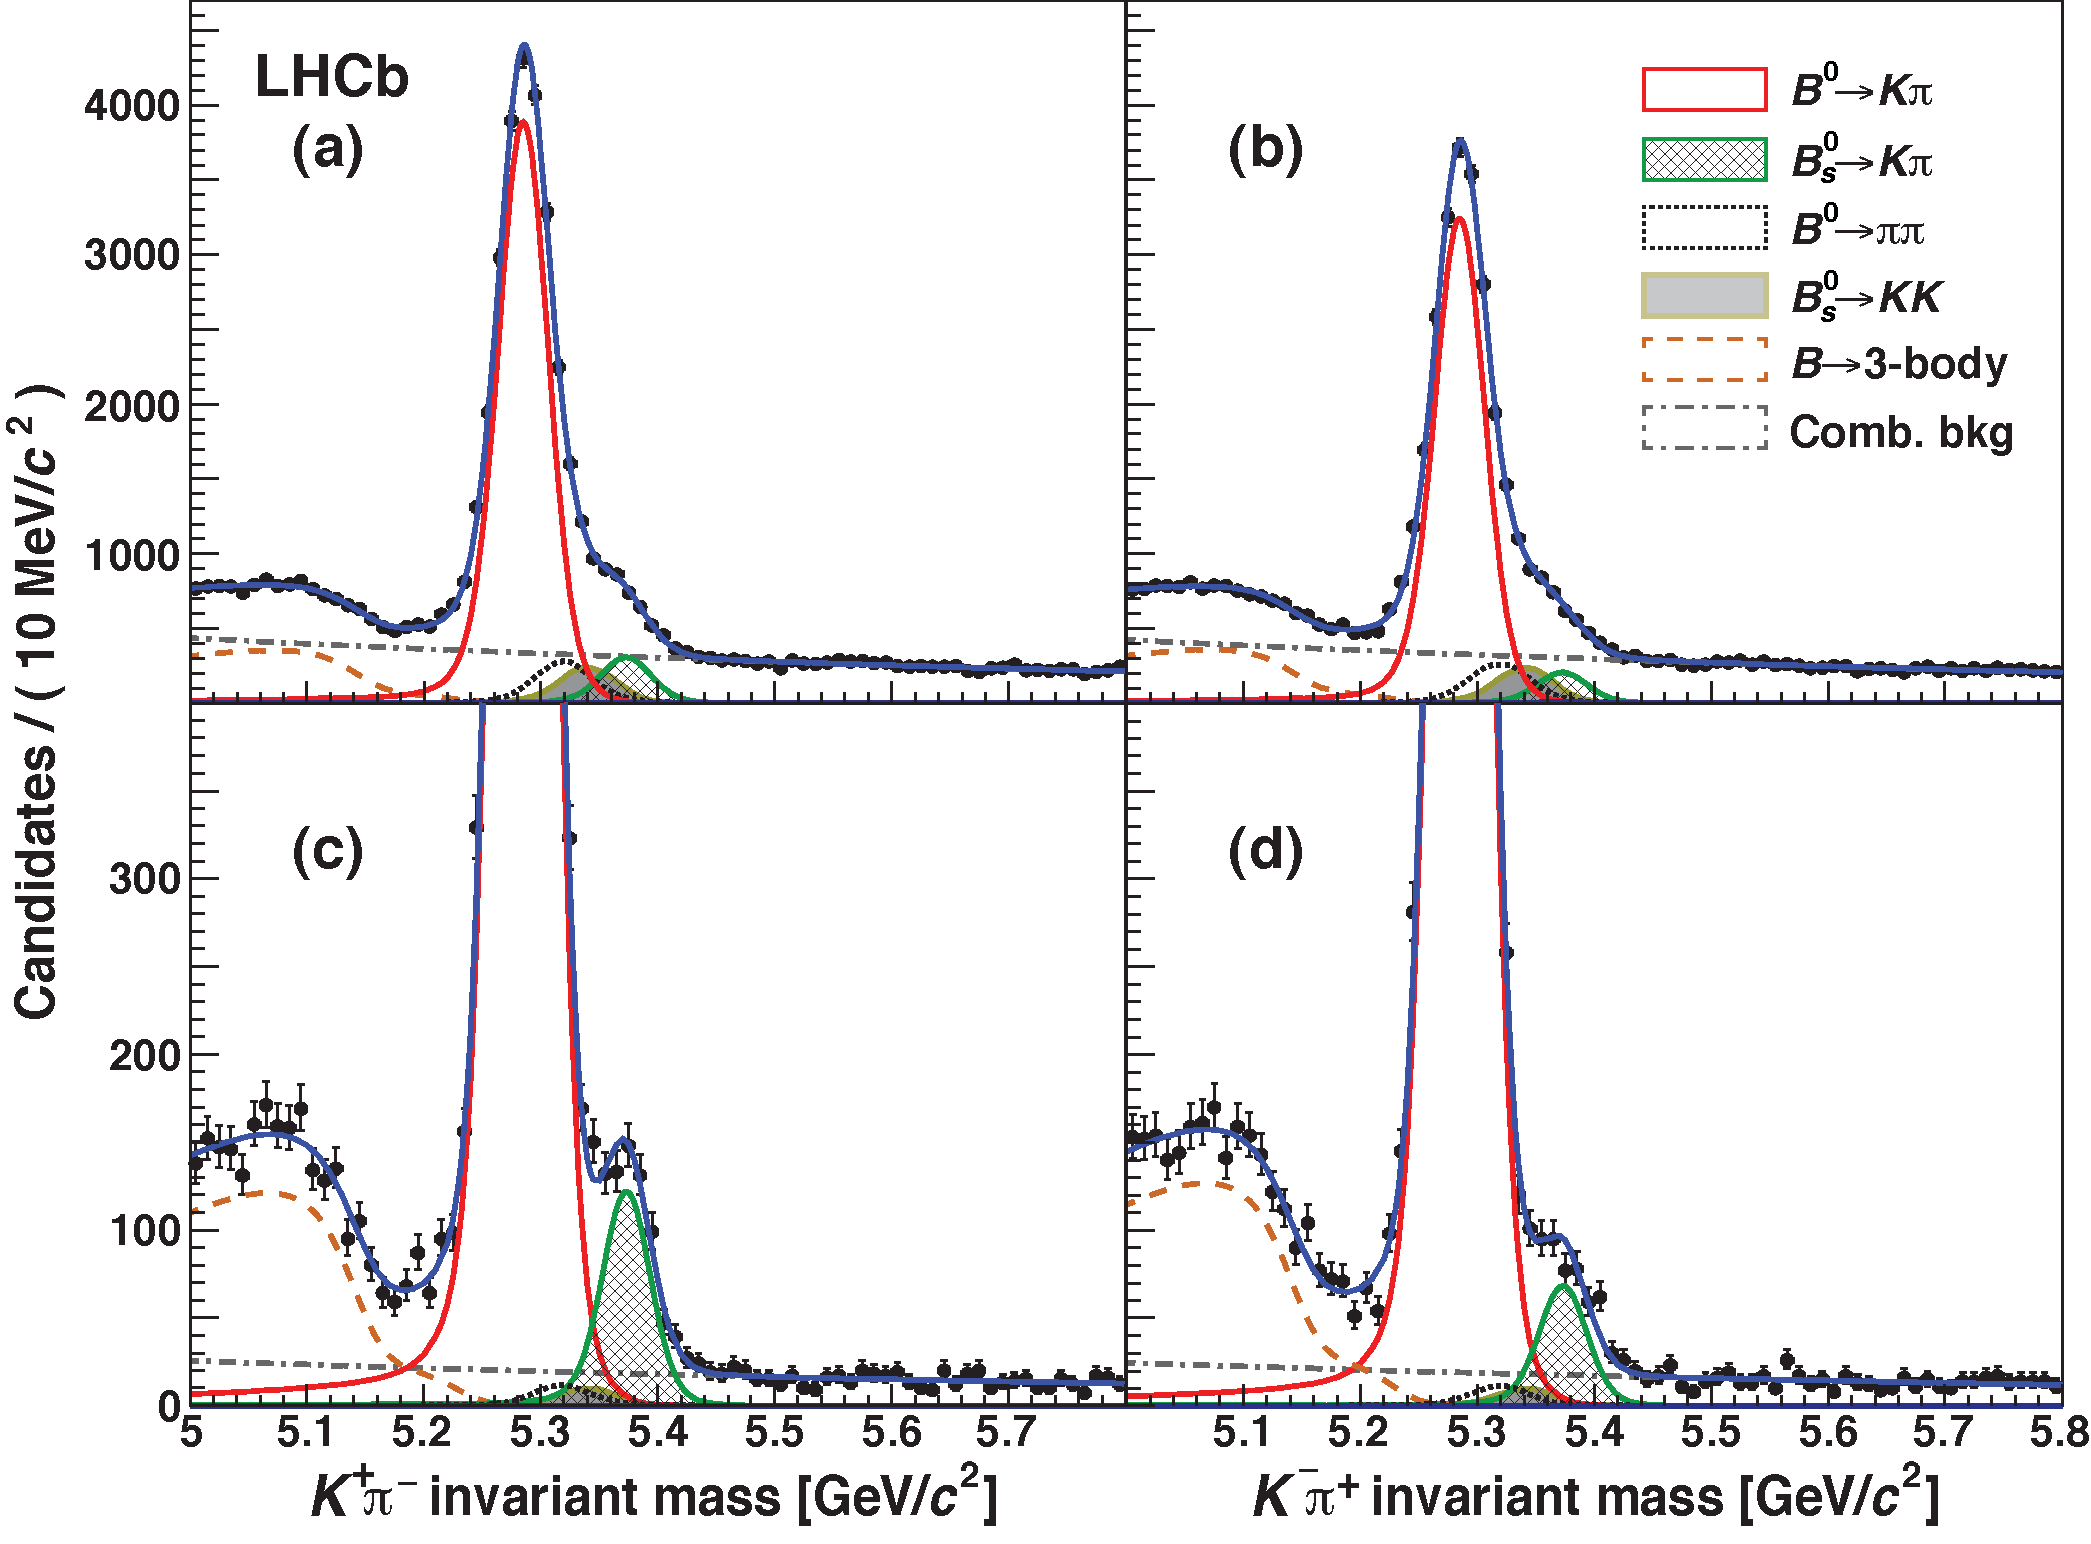
\includegraphics[width=0.8\textwidth]{03CPV/figs/DirectCPV.pdf}
	\caption{Invariant mass spectra obtained with the event selection for the best sensitivity on $A_{\CP}\left(\Bz\to\Kp\pim\right)$ (a,b) and $A_{\CP}\left(\Bs\to\Km\pip\right)$ (c,d). The figures (a) and (c) show the invariant mass distributions for \Kp\pim, figures (b) and (d) show the invariant mass distributions for \Km\pip.}
	\label{fig:DirectCPV}
\end{figure}


\subsection[head={Mixing \CP violation},tocentry={Mixing \CP violation}]{Mixing $\symbfsf{C{}P}$ violation}
\label{sec:MixingCPV}

Indirect \CP violation, also denoted as \CP violation in mixing implies that the transition probabilities for a \Bz-meson to oscilate into a \Bzb meson and vice versa are different.
As due to charge conservation mxing is only possible for uncharged mesons this type of \CP violation cannot occur for charged particles.
Using the time evolution from \cref{eq:timeEvolution} the probabilities of initially produced \Bz and \Bzb mesons to have oscillated within a proper-time $t$ are
\begin{align}
\left|\left<\Bz\Big|\Bzb\!\left(t\right)\right>\right|^2=\frac{1}{4}\left|\frac{p}{q}\right|^2
\left(e^{-\GH t}+e^{-\GL t}-2e^{\frac{1}{2}\left(\Gamma\right)t}\cos\left(\dm t\right)\right),\\
\left|\left<\Bzb\Big|\Bz\!\left(t\right)\right>\right|^2=\frac{1}{4}\left|\frac{q}{p}\right|^2
\left(e^{-\GH t}+e^{-\GL t}-2e^{\frac{1}{2}\left(\Gamma\right)t}\cos\left(\dm t\right)\right).
\end{align}
To obtain the same probabilities for both processes obviously
\begin{equation}
\left|\frac{q}{p}\right|=\left|\frac{p}{q}\right| \Rightarrow \left|\frac{q}{p}\right|=1
\end{equation}
is required.
According to \cref{eq:qoverp} this means that indirect \CP violation occurs if the matrix elements $m_{12}$ and $\Gamma_{12}$ have different complex phases.
The \CP asymmetry in case of indirect \CP violation can be defined as
\begin{equation}
A_{\CP}(t)=\frac{\Gamma\left(\Bz\to\Bzb\right) - \Gamma\left(\Bzb\to\Bz\right)}{\Gamma\left(\Bz\to\Bzb\right) + \Gamma\left(\Bzb\to\Bz\right)}
= \frac{1-\left|\nicefrac{p}{q}\right|^4}{1+\left|\nicefrac{p}{q}\right|^4}
\end{equation}
However, as neutral \B-mesons do not just oscillate but also decay this asymmetry can not be used directly to measure \CP violation in mixing.
Instead the \B-mesons need to be reconstructed in flavour specific decays, \ie only the transitions $\Bz\to\f$ and $\Bzb\to\fbar$, but not $\Bz\to\fbar$ and $\Bzb\to\f$ are allowed.
Thus the flavour of the meson at decay can be determined by final state and compared to the initial production flavour.
For the \Bz and \Bs meson system \CP violation in mixing has been measured to be negligible \cite{HFLAV2016} what is in good agreement with the \ac{SM} predictions.

\subsection[head={Interference \CP violation},tocentry={Interference \CP violation}]{Interference $\symbfsf{C{}P}$ violation}
\label{sec:InterferenceCPV}

So far \CP violation arising due to a clash between the phases of two interfering decay amplitudes or a clash between the phases of $m_{12}$ and $\Gamma_{12}$ has been discussed.
The third possibility is a clash between the phase of $\nicefrac{q}{p}$ and the phase of the decay amplitude what results in the so-called interference \CP violation.
For this class of \CP violation decays of \Bz and \Bzb mesons into both the final state \f and its \CP-conjugate \fbar need to be considered.

Inverting the requirement for \CP violation in mixing shows that \CP is conserved when there is a phase $\xi'$ such that
\begin{equation}
\begin{split}
m_{12}^\ast &= e^{2i\xi'}m_{12}\\
\Gamma_{12}^\ast &= e^{2i\xi'}\Gamma_{12}\label{eq:CPconservationMixing}
\end{split}
\end{equation}
what leads directly to $\nicefrac{q^2}{p^2} = e^{2i\xi'}$.
Using \cref{eq:CPTransInitFinal} the \CP conjugated amplitudes \Abarfbar and \Afbar can be expressed as
\begin{align}
\Abarfbar&=e^{i\left(\xi_f-\xi\right)}\Af,\label{eq:amplitudetransformation_1}\\
\Afbar&=e^{i\left(\xi_f+\xi\right)}\Abarf.\label{eq:amplitudetransformation_2}
\end{align}
what leads to $\big|\,\Af\,\big|=\big|\,\Abarfbar\,\big|$ and $\big|\,\Abarf\,\big|=\big|\,\Afbar\,\big|$ after eliminating the phases and shows that these amplitudes are \CP conserving.
Combining \cref{eq:amplitudetransformation_1} and \cref{eq:amplitudetransformation_2} then leads to
\begin{equation}
\Af\,\Afbar=e^{2i\xi}\,\Abarfbar\,\Abarf\,.
\end{equation}
Under the assumption that the phase of $\nicefrac{q}{p}$ and the phases of the decay amplitudes do not clash, \ie $\xi=\xi'$, \CP is conserved and
\begin{equation}
\arg\left(\frac{p^2}{q^2}\Af \,\overline{\kern -1.0pt A\kern -1.0pt}_{\kern 1.0pt f}^\ast\,\Afbar\overline{\kern -1.0pt \,A\kern -1.0pt}_{\kern 2.5pt\overline{\kern -1.5pt f\kern 1.5pt}}^\ast\right)=0
\end{equation}
applies.
This can be reformulated using the parameters
\begin{equation}
\Lf=\frac{q}{p}\frac{\Abarf}{\Af}\hspace{0.5cm}\text{and}
\hspace{0.5cm}\Lfbar=\frac{p}{q}\frac{\Afbar}{\Abarfbar}.
\end{equation}
Even without \CP violation in decay or mixing ($\big|\Lf\big|=\big|\Lfbar\big| = \pm1$) \CP is not conserved in case of
\begin{equation}
	\arg\left(\Lf\right)-\arg\left(\Lfbar\right)\neq0. \label{eq:conditionCPV}
\end{equation}

This type of \CP violation was first measured by the \B-factories \babar \cite{Aubert:2001nu} and \belle \cite{Abe:2001xe}.
The most prominent measurement is probably the anlysis of the so-called golden mode \BdToJPsiKS to determine $\sin{}\left(2\beta\right)$.
For this decay channel the condition in \cref{eq:conditionCPV} can be simplified to $\arg\left(\Lf\right)\neq0$ as only one common finalstate for both \Bz and \Bzb exists.
Furthermore no \CP violation in decay and mixing is expected for the decay \BdToJPsiKS and with the current experimental precision $\DG=0$ can be assumed.
Therefore the \CP asymmetry can be expressed as
\begin{equation}
A_{\CP}(t)=\frac{\Gamma\left(\BdToJPsiKS\right)-\Gamma\left(\BdToJPsiKS\right)}{\Gamma\left(\BdToJPsiKS\right)+\Gamma\left(\BdToJPsiKS\right)}=\Sf\sin\left(\dmd t\right),
\end{equation}
with the parameter $\Sf=\sin{}\left(2\beta\right)$ (a more thoroughly description of the formalism will be given in \cref{ch:CKMAngleGamma}).
The most recent measurement of \Sf was performed by \lhcb \cite{Aaij:2015vza} yielding a result of
\begin{equation}
\Sf=0.731\pm0.035\stat0.005\syst,
\end{equation}
what is consistent with the \ac{SM} expectations. The resulting \CP asymmetry is shown in \cref{fig:sin2beta}
\begin{figure}[tbp]
	\centering
	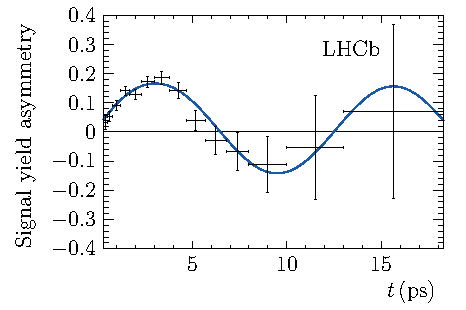
\includegraphics[width=0.6\textwidth]{03CPV/figs/InterferenceCPV.pdf}
	\caption{Time-dependent signal yield asymmetry $\left(N_{\Bzb}-N_{\Bz}\right)/\left(N_{\Bzb}-N_{\Bz}\right)$. The black points represent the used datasample, the solid curve is the projection of the signal \PDF.}
	\label{fig:sin2beta}
\end{figure}

  % % !TEX root = main.tex
\chapter[head={The CKM angle $\gamma$},tocentry={The CKM angle $\symbfsf{\gamma}$}]{The CKM angle $\symbfsf{\gamma}$}
\label{ch:CKMAngleGamma}

As mentioned before overconstraining the triangle relations following from the unitarity of the matrix is a nice experimental self consistency check of the \ac{SM}.
The CKM angle $\gamma$ is one of five observables parametrising the CKM triangle described in \cref{eq:CKMtriangle}.
The current experimental constraints on this triangle are shown in \cref{fig:ckmtriangle}.
One can see that $\gamma$ is currently the least well known parameter.
Hence, a more accurate determination of $\gamma$ is one of the main tasks of current research in the field of flavour physics.
This chapter is organised as follows: Firstly it is described how $\gamma$ in general can be accessed in section \cref{sec:accessGamma}, especially the determination using tree-level decays (\cref{sec:gamamInTrees}) and loop-processes (\cref{sec:gamamInLoops}) is emphasized, followed by the explanation how the decay mode \BdToDpi can be used to derive constraints on $\gamma$ in \cref{sec:GammaInBd2Dpi}.

\begin{figure}[tbp]
	\centering
	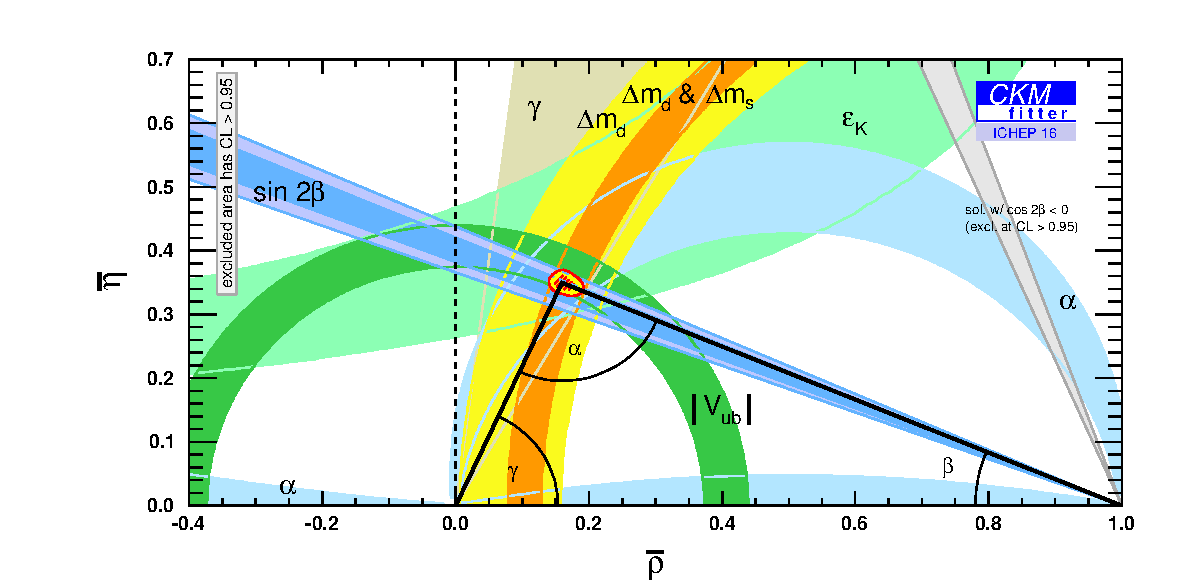
\includegraphics[width=0.8\textwidth]{04gamma/figs/CKMTriangle.pdf}
	\caption{CKM triangle in the complex plane.
	The coloured bands show the experimental constraints.
	The red hashed and the yellow area around the apex represent the currrent uncertainties at \SI{68}{\percent} and \SI{95}{\percent} confidence level, respectively~\cite{CKMfitter2015}.}
	\label{fig:ckmtriangle}
\end{figure}

\section[head={Accessing the angle $\gamma$},tocentry={Accessing the angle $\gamma$}]{Accessing the angle $\symbfsf{\gamma}$}
\label{sec:accessGamma}


As can be seen from the from in \cref{eq:CKMangles} the angle $\gamma$ is the only angle which is independent of CKM elements involving the top quark.
This makes it the only angle, which can be determined theoretically clean from tree-level decays.
On the other hand the experimental challenges are huge as transitions sensitive to $\gamma$ need to be proportional to \Vub, \ie such transitions are highly suppressed by order $\mathcal(O)\left(\lambda^3\right)$.
So either the precision of single measurements is limited due to small interference effects and branching fractions or in addition to the tree-level transition also penguin contributions of similar size contribute.
These gluonic penguins usually carry a weak phase different from the one in the tree-level diagram.

This latter possibility is briefly discussed using the example of the $\Bs\to\rho\KS$ decay.
Similar to the case of the golden mode \BdToJPsiKS, $\rho\KS$ is a \CP eigenstate and only the parameter \Lf needs to be calculated.
Using the amplitudes
\begin{equation}
\begin{aligned}
\Af&=\left<\rho\KS\left|T\right|\Bs\right>=-\frac{1}{2q_{\kaon}}\left<\rho\Kzb\left|T\right|\Bs\right>=-\frac{1}{2q_{\kaon}}\Vubst\Vud\\
\Abarf&=\left<\rho\KS\left|T\right|\Bsb\right>=\frac{1}{2p_{\kaon}}\left<\rho\Kz\left|T\right|\Bsb\right>=\frac{1}{2p_{\kaon}}\Vub\Vudst
\end{aligned}
\end{equation}
where $q_{\kaon}$ and $p_{\kaon}$ are the same mixing parameters for the neutral kaon system as shwon in \cref{eq:qoverp} for the \Bz-meson system.
With $\nicefrac{q_{\kaon}}{p_{\kaon}}=\nicefrac{\Vcsst\Vcd}{\Vcs\Vcdst}$ the parameter \Lf can be expressed in terms of the CKM matrix elements
\begin{equation}
\Lf=-\frac{q_{\kaon}}{p_{\kaon}}\frac{q}{p}\frac{\left<\rho\Kz\left|T\right|\Bsb\right>}{\left<\rho\Kzb\left|T\right|\Bs\right>}
=-\frac{\Vcsst\Vcd}{\Vcs\Vcdst}\frac{\Vtbst\Vts}{\Vtb\Vtsst}\frac{\Vub\Vudst}{\Vubst\Vud}.
\end{equation}
Using the Wolfenstein paramtrisation as shown in \cref{eq:CKMmatrix} this simplifies \Lf being a pure phase
\begin{equation}
\Lf=e^{-2i\gamma}.
\end{equation}
For $\Bs\to\rho\KS$ the finalstate $\rho$ has a \uquark\uquarkbar and a \dquark\dquarkbar component.
This means that alongside the spectator \squark-quark not only the tree-level transition $\bquark\to\uquark\uquarkbar\dquarkbar$ but also the gluonic-penguin transition $\bquark\to\dquark\dquarkbar\dquarkbar$ is possible (see \cref{fig:Bs2RhoKS}).
\begin{figure}[tbp]
	\centering
	\includestandalone{04gamma/figs/BsToRhoKS_Tree}
	\includestandalone{04gamma/figs/BsToRhoKS_Penguin}
	\caption{Tree-level diagram of $\Bs\!\to\rho\KS$ (left) and the dominantly contributing gluonic penguin (right). \cite{Ellis:2016jkw}.}
	\label{fig:Bs2RhoKS}
\end{figure}
For both diagrams the CKM-factor is $\propto A\lambda^3$, but the weak phases are $\gamma$ and $\beta$ for the tree-level diagram and the penguin, respectively.
The effect of an additional contributing amplitude with a weak phase differing from the one of the tree-level process can be quantified.
Considering two weak phases contributing to the transitions \Af ($\Bs\to\rho\KS$) and \Abarf ($\Bsb\to\rho\KS$):
\begin{equation}
\begin{aligned}
\Af&=A_1e^{i\left(\Phi_{A_1}+\delta_1\right)}+A_2e^{i\left(\Phi_{A_2}+\delta_2\right)}\\
\Abarf&=\eta_f\left[A_1e^{i\left(-\Phi_{A_1}+\delta_1\right)}+A_2e^{i\left(-\Phi_{A_2}+\delta_2\right)}\right]
\end{aligned}
\end{equation}
As shown in \cref{eq:qoverPPurePhase} the quantity $\nicefrac{q}{p}$ is a pure phase and hence one can write $\nicefrac{q}{p}=-e^{2i\Phi_\text{M}}$, what leads to
\begin{equation}
\Lf=-\eta_f\,e^{2i\Phi_\text{M}}\frac{ A_1 e^{i\left(-\Phi_{A_1}+\delta_1\right)} + A_2 e^{i\left(-\Phi_{A_2}+\delta_2\right)}}{A_1e^{i\left(\Phi_{A_1}+\delta_1\right)}+A_2e^{i\left(\Phi_{A_2}+\delta_2\right)}} \label{eq:LfWithPenguin}
\end{equation}
with the \emph{weak} and \emph{strong} phases $\Phi_{A_i}$ and $\delta_i$, respectively.
The phases $\Phi_{A_1}$, $\Phi_{A_2}$ and $\Phi_\text{M}$ are not rephasing-invariant, but the relative phases $\Phi_1\equiv\Phi_{A_1}-\Phi_\text{M}$, $\Phi_2\equiv\Phi_{A_2}-\Phi_\text{M}$ and $\Delta=\delta_2-\delta_1$ can be measured.
For $\Bs\to\rho\KS$ one can \eg identify $A_1$ and $A_2$ with amplitude corresponding to the tree-level and gluonic-penguin diagram, respectively.
Accordingly the phase $\Phi_1$ and $\Phi_2$ would represent the CKM angles $\gamma$ and $\beta$.
Already the form of $\Lf$ in \cref{eq:LfWithPenguin} shows that the penguin contribution in $\Bs\to\rho\KS$ makes it impossible to measure $\gamma$
However this case might be extrem in the sense that both amplitudes are of the same magnitude.
But even with the approximation that $r=\nicefrac{A_2}{A_1}$ is small one finds
\begin{align}
\Lf&=-\eta_fe^{-2i\Phi_1}\frac{1+re^{i\left(\Delta-\Phi_2+\Phi_1\right)}}{1+re^{i\left(\Delta+\Phi_2-\Phi_1\right)}}\nonumber\\
&\approx-\eta_fe^{-2i\Phi_1}\left[1+2r\sin\Delta\sin\left(\Phi_2-\Phi_1\right)-2ir\cos\Delta\sin\left(\Phi_2-\Phi_1\right)\right].
\end{align}
Obviously in case a guonic-penguin contributes with a different weak phase from that of the tree-level diagram - \ie $r\neq0$ and $\Phi_1\neq\Phi_2$ - it is not possible to measure a single weak phase.
Now one finds, that in case a second penguin with a different weak phase from that of the tree-level diagram contributes the parameter and $r\neq0$, \Lf does not allow to measure a single weak phase.
Even in the case of vanishing final state interactions, \ie $\Delta=0$, \Lf can just be written as
\begin{equation}
\Lf=-\eta_fe^{-2i\left(\Phi_1-\delta_{\Phi_1}\right)}
\end{equation}
where $\delta_{\Phi_1}$ is defined by
\begin{equation}
\tan\left(\delta_{\Phi_1}\right)=\frac{r\sin\left(\Phi_1-\Phi_2\right)}{1+r\cos\left(\Phi_1-\Phi_2\right)}.
\end{equation}
Additionally it is important to note that hadronic matrix elements cannot be calculated reliably.
This means that in case they do not cancel out as they do if only one amplitude contributes to a specific decay, the resulting \CP asymmetries cannot be interpreted without large uncertainties which need to be propagated into the determination of the sides and angles of the unitarity triangle.

Therefore the current strategy to decrease the uncertainty on $\gamma$ is to measure it in many different decay modes and combine the results afterwards.
These decay modes can be divided into the two mentioned classes: The first class are tree-level processes where either decays of charged \B mesons or neutral \B mesons are exploited.
The second class are processes involving penguin contributions, \eg similar to the contribution to $\Bs\to\rho\KS$ described above.

\subsection[head={Determination of $\gamma$ in tree-level decays},tocentry={Determination of $\gamma$ in tree-level decays}]{Determination of $\symbfsf{\gamma}$ in tree-level decays}
\label{sec:gamamInTrees}

% In the \ac{SM} two types of \CP violation, namely direct and interference \CP violation, are expected to a non-negligible amount.
As $\gamma$ is propotional to the phase of the matrix element \Vub a natural way to measure it is to exploit interference effects between the Cabibbo-favoured $\bquark\to\cquark$ transitions and the Cabibbo-suppressed $\bquark\to\uquark$ transitions in decay channels such as $\Bu\to\D\Kp$ and \BsToDsK.
In the first case exploring different \D decay chaines requires slightly different experimental methods, whereas in the latter case a time-dependent analysis is needed.

The basic principle when exploiting decays of charged \B mesons is always the same.
The initial \Bpm meson decays into \Dz\Kpm or \Dzb\Kpm and subsequently the \D meson is reconstructed in a final state common to both \Dz and \Dzb.
Therefore the amplitudes for the decay of the \B meson can be defined as
\begin{equation}
\begin{aligned}
A\!\left(\Bp\!\to\Dz\Kp\right)&=\Vubst\Vcs=Ae^{i\left(\delta+\gamma\right)}\\
A\!\left(\Bp\!\to\Dzb\Kp\right)&=\Vcbst\Vus=\overline{\kern -1.0pt A\kern -1.0pt}\,e^{i\left(\overline{\delta}\right)}
\end{aligned}
\end{equation}
where the \emph{weak} phase was directly idenitified as $\gamma$, $\delta$ and $\overline{\delta}$ are the \emph{strong} phases and $A$ and $\overline{\kern -1.0pt A\kern -1.0pt}$ are the moduli of the amplitudes.
For the \D-meson decay the ampltiudes can be defined accordingly as
\begin{equation}
\begin{aligned}
A\!\left(\Dz\!\to\f\right)&=A_De^{i\left(\delta_D\right)}\\
A\!\left(\Dzb\!\to\f\right)&=\overline{\kern -1.0pt A\kern -1.0pt}_D\,e^{i\left(\overline{\delta}_D\right)}.
\end{aligned}
\end{equation}
Hence, the transition of $\Bp\to\f$ has two contributing amplitudes, which produce an interference term containing $\gamma$ in the total decay rate
\begin{equation}
\left|A\!\left(\Bp\!\to\f\,\Kp\right)\right|^2=A^2\overline{\kern -1.0pt A\kern -1.0pt}{}_D^2\left(1+r_\B^2r_\D^2+2\,r_\B r_\D\cos\left(\Delta+\Delta_\D+\gamma\right)\right)\label{eq:totDecRateChargedB}
\end{equation}
where the short notations $r_\B=\nicefrac{\overline{\kern -1.0pt A\kern -1.0pt}}{A}$, $r_\D=\nicefrac{A_\D}{\overline{\kern -1.0pt A\kern -1.0pt}_\D}$, $\Delta=\overline{\delta}-\delta$ and $\Delta_\D=\delta_\D-\overline{\delta}_\D$ were used.
To obtain the total decay rate for the \Bm decay just the sign of $\gamma$ must be reversed.

The first method exploiting this interference is the so-called GLW method \cite{GLW_1, GLW_2}.
The ideas is simply to reconstruct the intermediate \D meson in \CP eigenstates such as \Kp\Km (\CP-even) or \KS\piz (\CP-odd).
The consequences of such choice are that the unknowns from the \D decay can be reduced because $r_\D=1$ and $\Delta_\D=0$, so the total decay rates for \eg a \CP-even \D decay can be written as
\begin{equation}
\left|A\!\left(\Bpm\!\to f_{\CP}\Kpm\right)\right|^2=A^2A_\D^2\left(1+r_\B^2+2r_\B\cos\left(\Delta\pm\gamma\right)\right).\label{eq:totDecRateGLW}
\end{equation}
Experimentally for the \CP-even final state a \CP asymmetry
\begin{equation}
A_{\CP}^{\text{GLW}}=\frac{\left|A\!\left(\Bm\!\to f_{\CP}\Km\right)\right|^2-\left|A\!\left(\Bp\!\to f_{\CP}\Kp\right)\right|^2}{\left|A\!\left(\Bm\!\to f_{\CP}\Km\right)\right|^2+\left|A\!\left(\Bp\!\to f_{\CP}\Kp\right)\right|^2}=\frac{2r_\B\sin\left(\Delta\right)\sin\left(\gamma\right)}{1+r_\B^2+2r_\B\cos\left(\Delta\pm\gamma\right)}\label{eq:ACP_GLW}
\end{equation}
and a \CP ratio
\begin{equation}
R_{\CP}^{\text{GLW}}=\frac{\left|A\!\left(\Bm\!\to f_{\CP}\Km\right)\right|^2+\left|A\!\left(\Bp\!\to f_{\CP}\Kp\right)\right|^2}{2\left|A\!\left(\Bm\!\to\Dz\Km\right)\right|^2}=1+r_\B^2+2r_\B\cos\left(\Delta\right)\cos\left(\gamma\right)\label{eq:RCP_GLW}
\end{equation}
can be measured. If the \D meson in the denominator of $R_{\CP}^{\text{GLW}}$ is reconstructed in a hadronic final state as \kaon\pion decays proceeding via a \Dz or a \Dzb cannot distinguished as both decay into \Kp\pim and \Km\pip. However, this can be avoided by measuring instead the double ratio
\begin{equation}
R_{+}^{\text{GLW}}=\frac{\left|A\!\left(\Bm\!\to f_{\CP}\Km\right)\right|^2+\left|A\!\left(\Bp\!\to f_{\CP}\Kp\right)\right|^2}{\left|A\!\left(\Bm\!\to f_{\CP}\pim\right)\right|^2+\left|A\!\left(\Bp\!\to f_{\CP}\pip\right)\right|^2}\times\frac{1}{R_{\kaon/\pion}}
\end{equation}
with
\begin{equation}
R_{\kaon/\pion}=\frac{\left|A\!\left(\Bm\!\to \D\left(\to\Km\pip\right)\Km\right)\right|^2+\left|A\!\left(\Bp\!\to \D\left(\to\Kp\pim\right)\Kp\right)\right|^2}{\left|A\!\left(\Bm\!\to \D\left(\to\Km\pip\right)\pim\right)\right|^2+\left|A\!\left(\Bp\!\to \D\left(\to\Kp\pim\right)\pip\right)\right|^2}.
\end{equation}
This double ratio $R_{+}^{\text{GLW}}$ is identical to $R_{\CP}^{\text{GLW}}$ when neglecting all terms proportional to $r_\D$ or $r_{\B_\pion}=\nicefrac{A\!\left(\Bp\!\to\Dz\pip\right)}{A\!\left(\Bm\!\to\Dz\pim\right)}$.
However the GLW method has two disadvantages: Firstly, the interference term is proportional to $r_\B$ which is of order \SI{10}{\percent} and therefore decreases the sensitivity on $\gamma$.
Second, there is not only one solution for $\gamma$, but there is a eight-fold discrete ambiguity due to the fact that $\gamma$ and $\Delta$ always appear together in the product of two sine or cosine functions as in \cref{eq:ACP_GLW} and \cref{eq:RCP_GLW}.

The second method directly counteracts to the first disadvantage of the GLW method.
Instead of using decays into \CP-eigenstates of the \D meson, the \D is reconstructed in a final state for which $\Dz\!\to\f$ is suppressed relative to $\Dzb\!\to\f$ (\eg \f could be \Km\pip) \cite{ADS}.
This enhances the interference term to be of the same order as the other ones, but on the other hand the $r_\D$ and $\Delta_\D$ do not cancel as before.
Hence, to determine $\gamma$ from similar asymmetries and ratios as for the GLW method external input for both quantities is needed.

The last method described in this section using charged \B decays is probably the most sophisticated one.
The GGSZ method makes use of multibody \D decays.
This requires an analysis of the Dalitz plane, but on the other hand $\gamma$ can be extracted without the disadvantages of the GLW or the ADS method.
The basic idea however is the same as before, just that the strong phase originating from the \D decay varies over the Dalitz plane.
Furthermore, the interference term can be expressed in the form $\cos\!\left(\phi\right)c_i\pm\sin\!\left(\phi\right)s_i$, where $\phi$ is the difference (sum) of the \emph{strong} phase $\delta_\B$ originating from the \Bm (\Bp) decay and $\gamma$.
The coefficients $c_i$ and $s_i$ contain the \emph{strong} phases from the \D decay.
Using $k$ pairs of bins which are symmetrically around the $m_{\KS\pim}\leftrightarrow m_{\KS\pip}$ line in the Dalitz plot, and exploiting the symmetry of the $c_i$ and $s_i$ around this line leads to $4k$ equations.
This equations are related to the $2k+3$ unknowns $c_i$, $s_i$, $r_\B$, $\delta_\B$ and $\gamma$, so that a partition of the \D meson Dalitz plot into four or more bins allows to determine all unknowns.

Finally it is important to note, that the described techniques can be applied as well to any decays of type $\Bpm\!\to\D X^{\pm}$ where X is any state with the flavour of a \Kpm.

When exploiting decays of uncharged \B mesons such as \BsToDsK or \BdToDpi to determine the angle $\gamma$ the procedure is different.
This type of decays is only affected by interference \CP violation and therefore a time-dependent analysis is needed to achieve sensitivity at $\gamma$.
The basic formalism is already described in \cref{sec:formulaeCPV}.
Due to the \CP conservation in the decay, $\Cfbar=-\Cf$ and the number of independent coefficients as given in \cref{eq:cpcoeff} and \cref{eq:cpcoeffbar} is reduced to five.
Furthermore the \CP coefficient \Cf contains the ratio $r_\B$, while via the coefficients \Sf, \Sfbar, $A_f^{\DG}$, $A_{\kern 1.5pt\overline{\kern -1.5pt f\kern 1.5pt}}^{\DG}$ the phase information are measurable.
This experimental technique to measure \CP violation can be also applied to \BdToDpi and therefore it will be described more thouroughly in \cref{sec:GammaInBd2Dpi}.

\subsection[head={Determination of $\gamma$ in loop processes},tocentry={Determination of $\gamma$ in loop processes}]{Determination of $\symbfsf{\gamma}$ in loop processes}
\label{sec:gamamInLoops}
Instead of exploiting decays where $\gamma$ can be accessed via the interference in tree-level diagrams between the transitions $\bquark\to\uquark$ and $\bquark\to\cquark$ also processes containing loop transitions can be used to infer information about $\gamma$.
The first and probably most obvious possibility is to derive a result for $\gamma$ from experimental mesaurements of other CKM triangle quantities as the remaining two angles of the CKM triangle, $\alpha$ and $\beta$.
As an example the angle $\beta$ can be measured quite precisely in the decay \BdToJPsiKS while the angle $\alpha$ is accessible via Isospin analyses of the decays $\Bd\!\to\pip\pim$, $\Bd\!\to\piz\piz$ and $\Bu\!\to\pip\piz$ \cite{IsospinAlpha} or measurements of longitudinally polarized $\Bz\!\to\rho\rho$ decays \cite{alpha_BaBar, alpha_Belle}. Though, the best precision is achieved performing a \emph{full} fit using all available inputs as performed by the CKMfitter and UTfit collaborations \cite{CKMfitter2015, UTfit-UT}.

However such tests of a closing CKM triangle do not directly indicate certain processes that are affected effects of \ac{NP}.
Therefore, a more direct determination of $\gamma$ is also important.
A possibility for such determination is to extract $\gamma$ from \CP violation measurements in $B\!\to\pion\pion$ and $\Bs\!\to\Kp\Km$ \cite{GammaInLoops_Fleischer, GammaInLoops_Ciuchini}.
To do this, the U-spin flavour symmetry of strong interactions between the two decay channels - \ie the decays are related by interchanging all \dquark-quarks with \squark-quarks - must be used.
\begin{figure}[tbp]
	\centering
	\includestandalone{04gamma/figs/GammaLoopsTree}
	\hfill
	\includestandalone{04gamma/figs/GammaLoopsPenguin}
	\caption{Feynman diagrams contributing to $\Bd\!\to\pip\pim$ ($\quark=\dquark$) and $\Bs\!\to\Kp\Km$($\quark=\squark$) \cite{Ellis:2016jkw}.}
	\label{fig:feynmanGammaLoops}
\end{figure}

To briefly outline the strategy first the transition amplitudes and \CP observables for the decay modes $\Bz\!\to\pip\pim$ and $\Bs\!\to\Kp\Km$ will be introduced in the following:
In \cref{fig:feynmanGammaLoops} the dominant $\bquark\!\to\uquarkbar\uquark\dquarkbar$ processes are shown, which leads to the transition amplitude
\begin{equation}
A\!\left(\Bd\!\to\pip\pim\right)=\lambda_\uquark\left(A_{\text{cc}}^\uquark+A_{\text{pen}}^\uquark\right)+\lambda_\cquark A_{\text{pen}}^\cquark+\lambda_\tquark A_{\text{pen}}^\tquark
\end{equation}
where the amplitudes $A_{\text{pen}}^\quark$ and $A_{\text{c}}^\quark$ describe the penguin and charged-current contributions respectively.
Furthermore the short notation $\lambda_\quark=V_{{\kern -0.1em}\quark\dquark}V^{*}_{{\kern -0.1em}\quark\bquark}$ was used.
Making use of the unitarity of the CKM matrix and applying the Wolfenstein parametrisation \cite{Wolfenstein:1983yz} allows to determine the parameter \Lf and the corresponding \CP coefficients
\begin{equation}
\begin{aligned}
C_{f}^{\Bd\!\to\pip\pim}&=-\left[\frac{2d\sin\!\left(\theta\right)\sin\!\left(\gamma\right)}{1-2d\cos\!\left(\theta\right)\cos\!\left(\gamma\right)+d^2}\right]\\
S_{f}^{\Bd\!\to\pip\pim}&=\left[\frac{\sin\!\left(2\beta+2\gamma\right)-2d\cos\!\left(\theta\right)\sin\!\left(2\beta+\gamma\right)+d^2\sin\!\left(2\beta\right)}{1-2d\cos\!\left(\theta\right)\cos\!\left(\gamma\right)+d^2}\right].
\end{aligned}
\end{equation}
The quantities $d$ and $\theta$ are defined as
\begin{equation}
de^{i\theta}=\frac{1}{\left(1-\nicefrac{\lambda^2}{2}\right)R_b}\left(\frac{A_{\text{pen}}^{\cquark\tquark}}{A_{\text{cc}}^{\uquark}+A_{\text{pen}}^{\uquark\tquark}}\right)
\end{equation}
with $A_{\text{pen}}^{\quark\tquark}=A_{\text{pen}}^{\quark}-A_{\text{pen}}^{\tquark}$ and the CKM factor $R_b=\nicefrac{1}{\lambda}\left|\nicefrac{\Vub}{\Vcb}\right|$.
The \CP coefficient $A_f^{\DG}$ is neglected as the decay width difference for \Bd mesons is expected to be negligibly small.

Equivalent to this, the \CP coefficients for $\Bs\!\to\Kp\Km$ can be calculated as
\begin{equation}
\begin{aligned}
C_{f}^{\Bs\!\to\Kp\Km}&=\left[\frac{2\tilde{d'}\!\sin\!\left(\theta'\right)\sin\!\left(\gamma\right)}{1-2\tilde{d'}\!\cos\!\left(\theta'\right)\cos\!\left(\gamma\right)+\tilde{d'}^2}\right]\\
S_{f}^{\Bs\!\to\Kp\Km}&=\left[\frac{\sin\!\left(\phi_\squark+2\gamma\right)-2\tilde{d'}\!\cos\!\left(\theta\right)\sin\!\left(\phi_\squark+\gamma\right)+\tilde{d'}{}^2\!\sin\!\left(\phi_\squark\right)}{1-2\tilde{d'}\!\cos\!\left(\theta'\right)\cos\!\left(\gamma\right)+\tilde{d'}{}^2}\right]\\
A_f^{\DG, \Bs\!\to\Kp\Km}&=-\left[\frac{\cos\!\left(\phi_\squark+2\gamma\right)+2\tilde{d'}\!\cos\!\left(\theta'\right)\cos\!\left(\phi_\squark+\gamma\right)+\tilde{d'}{}^2\cos\!\left(\phi_\squark\right)}{1-2\tilde{d'}\!\cos\!\left(\theta'\right)\cos\!\left(\gamma\right)+\tilde{d'}{}^2}\right]
\end{aligned}
\end{equation}
where the short notation $\tilde{d'}=\left(\nicefrac{1-\lambda^2}{\lambda^2}\right)d'$ was used.
Assuming the U-spin flavour symmetry to be exact even implies that $d'=d$ and $\theta'=\theta$.

This theoretical setup can now be used in several strategies to determine $\gamma$ among other observables as $\beta$, $d$ and $\theta$.
In the following the basic idea of most strategies will be outlined briefly.
In the first approach the phase $\phi_s$ is taken as an external input, thus the four unknows $d$, $\theta$, $\beta$ and $\gamma$ can be determined using only the four observables $C_{f}^{B\!\to hh}$, and $S_{f}^{B\!\to hh}$.
As shown in \cite{GammaInLoops_Fleischer}, the coefficient the parameters $d$ and $\theta$ can be expressed as functions of $\gamma$, $C_{f}^{\Bs\!\to\Kp\Km}$ and $S_{f}^{\Bs\!\to\Kp\Km}$.
Inserting this into $C_{f}^{\Bd\!\to\pip\pim}$ allows then to determine $\gamma$ up to a two-fold ambiguity as shown in \cref{fig:gamma_beta_fleischer}.
\begin{figure}[tbp]
	\centering
	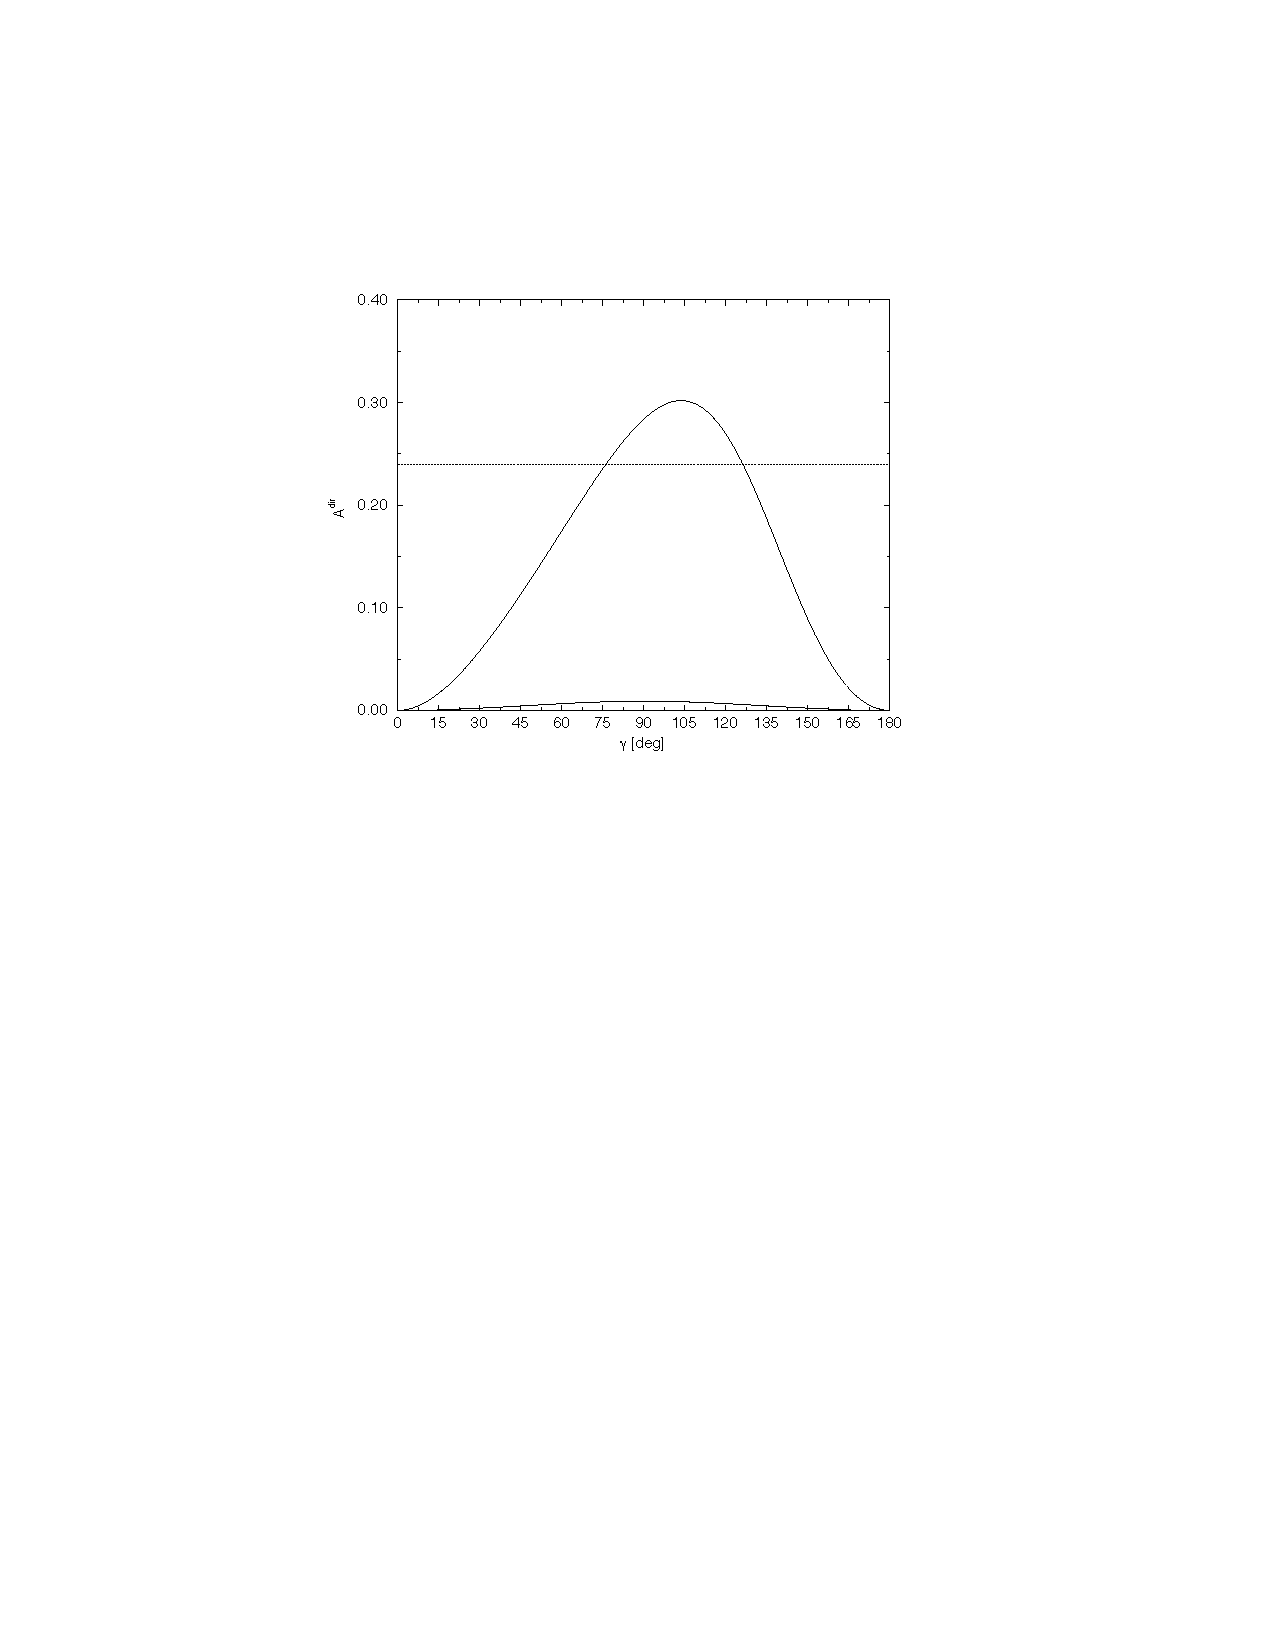
\includegraphics[width=0.4\textwidth]{04gamma/figs/GammaVsCf.pdf}
	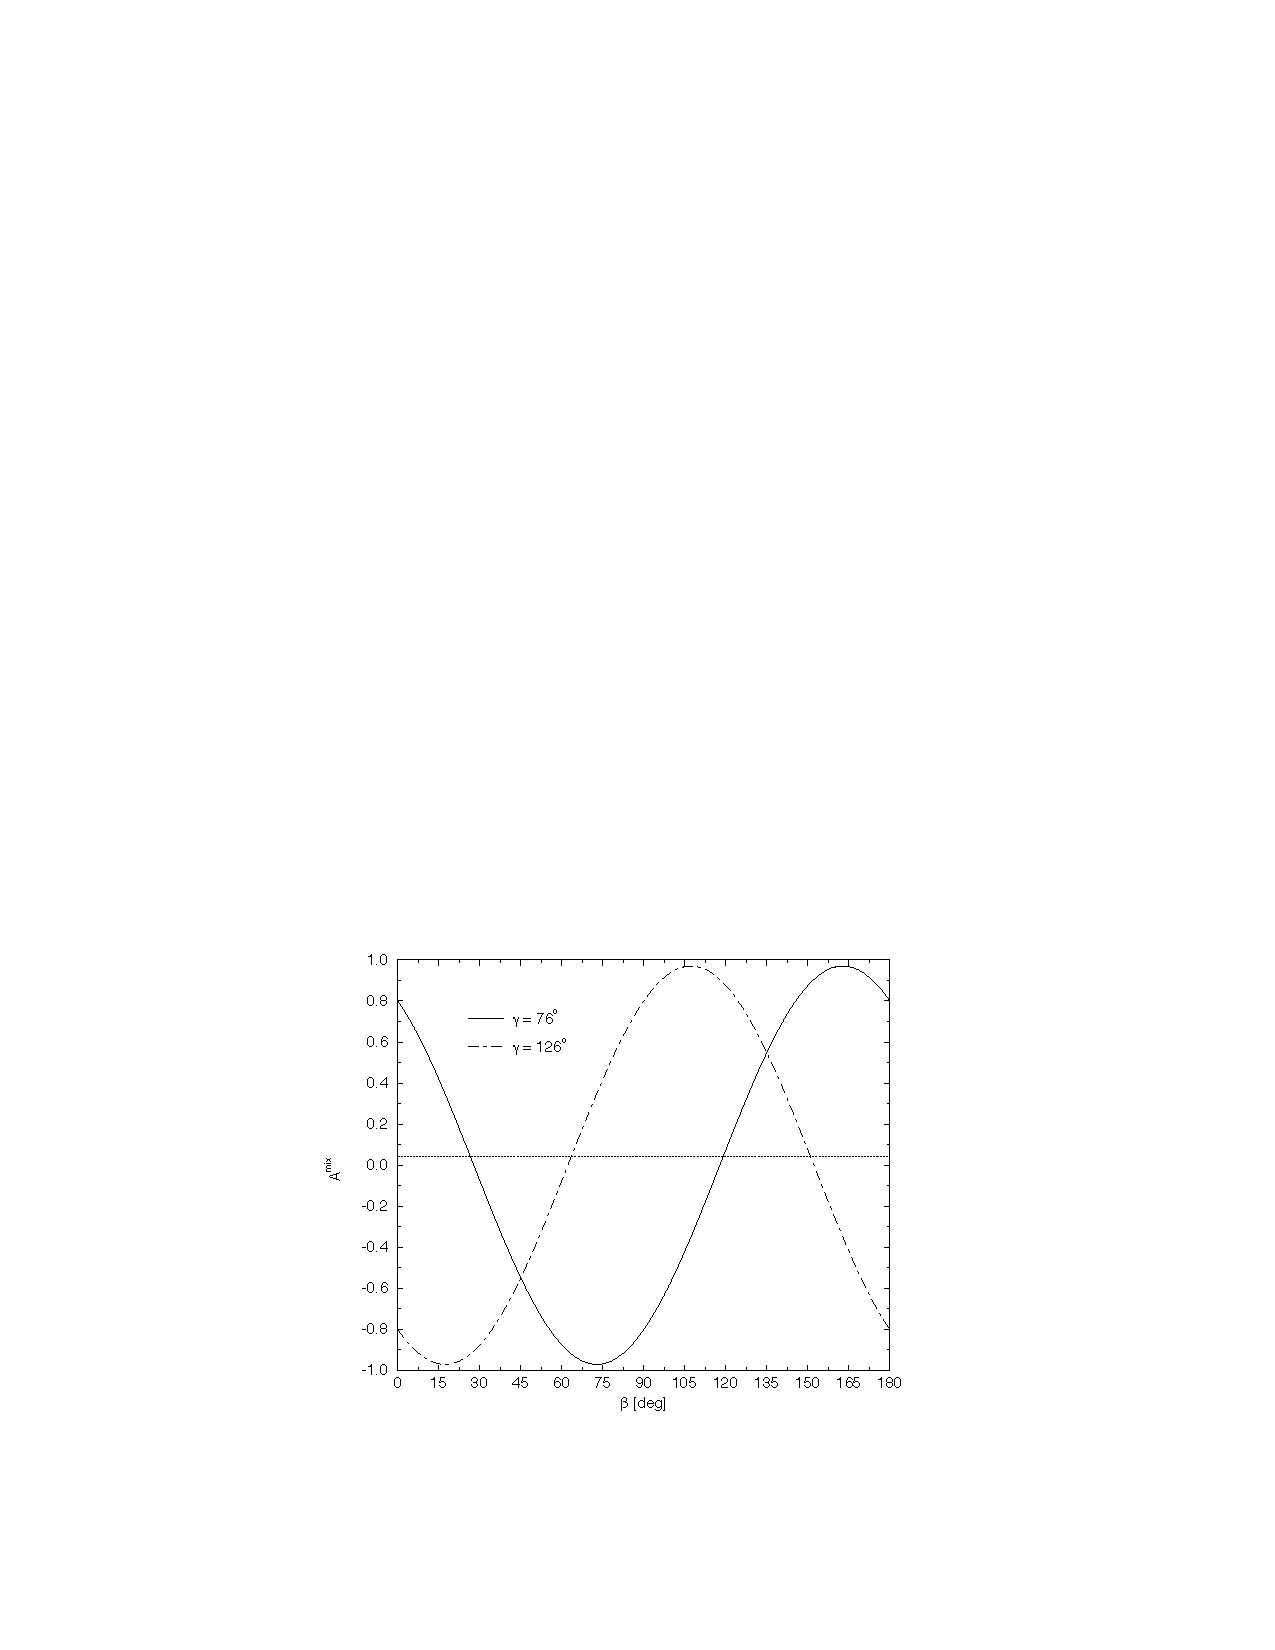
\includegraphics[width=0.4\textwidth]{04gamma/figs/BetaVsSf.pdf}
	\caption{Dependence of $C_{f}^{\Bd\!\to\pip\pim}$ ($A^{\text{dir}}$) on $\gamma$ (left) and $S_{f}^{\Bd\!\to\pip\pim}$ ($A^{\text{mix}}$) on $\beta$ for a specific example as given in \cite{GammaInLoops_Fleischer}.}
	\label{fig:gamma_beta_fleischer}
\end{figure}
Using these two solutions for $\gamma$ and inserting them together with the obtained expressions for $d$ and $\theta$ into $S_{f}^{\Bd\!\to\pip\pim}$ gives additionally a fourfold ambiguity for $\beta$ (see \cref{fig:gamma_beta_fleischer}).
Hereby for both ambiguities the assumption is made, that $\gamma\in[0, 180]\si{\degree}$ and $\beta\in[0, 180]\si{\degree}$.
If additionally the phase $\beta$ is used this ambiguities can be resolved by expressing $d$ and $\theta$ as functions of $\gamma$, $C_{f}^{\Bd\!\to\pip\pim}$ and $S_{f}^{\Bd\!\to\pip\pim}$ and consequently fixing the contours in the $\gamma-d$ plane.
However assuming a \SI{15}{\percent} and \SI{20}{\percent} U-spin-breaking effect on the parameters $d$ and $\theta$, respectively, an additional uncertainty on the extracted value of $\gamma$ of roughly \SI{20}{\percent} could arise \cite{GammaInLoops_Fleischer2}.
Adding also the modes $\Bd\!\to\piz\piz$ and $\Bu\!\to\piz\pip$ allows additionally to either constrain \ac{NP} effects in the $\bquark\!\to\squark$ penguin contributions or in mixing \cite{GammaInLoops_Ciuchini}.

\subsection[head={Comparison of tree-level and loop determinations of $\gamma$},tocentry={Comparison of tree-level and loop determinations of $\gamma$}]{Comparison of tree-level and loop determinations of $\symbfsf{\gamma}$}

Both strategies described in the previous two section were and are used to determine the angle $\gamma$.
As was shown the the determination from tree-level decays provides theoretically clean measurements, only affected by low sensitivity or discrete ambiguities.
Comparing these measurements with determinations using loop-processes could provide an effective handle on \ac{NP} effects contributing.
However to properly compare the different approaches, the experimental uncertainties need to be reduced to a sensible amount; therefore the current experimental status and required improvements in the experimental precision will be given below.

At \lhcb the potential of determination via tree-level processes was studied in many different final states and is combined on a regular basis into one single $\gamma$-combination. The most recent combination was presented in \cite{GammCombo} yielding a result of
\begin{equation}
\gamma=\left(74.0^{+5.0}_{-5.8}\right)\!\si{\degree}.\label{eq:gammaResult_Trees}
\end{equation}
This result includes \num{15} different decay modes, of which ten were analysed using data correspionding to \SI{3}{\per\femto\barn} collected at centre-of-mass energies of \num{7} and \SI{8}{\tera\electronvolt} and five additionally using data corresponding to \SI{2}{\per\femto\barn} collected at centre-of-mass energies of \SI{13}{\tera\electronvolt}.
Deriving constraints on $\gamma$ by performing a \emph{full} fit using all available inputs yields
\begin{equation}
\gamma=\left(65.4^{+0.97}_{-1.16}\right)\!\si{\degree}\,\,\,\,\,\text{and}\,\,\,\,\,\gamma=\left(65.8\pm1.9\right)\!\si{\degree}
\end{equation}
performed by the CKMfitter~\cite{CKMfitter2015} and UTfit~\cite{UTfit-UT} collaborations, respectively.
Determining $\gamma$ with a similar strategy exploiting U-spin-symmetry as outlined in \cref{sec:gamamInLoops} yields
\begin{equation}
\gamma=\left(63.5^{+7.2}_{-6.7}\right)\!\si{\degree}.\label{eq:gammaResult_Loops}
\end{equation}
where inputs from \babar, \belle, \cdf and \lhcb were used~\cite{Aaij:2014xba}. In contrast to the combination of tree-level measurements, the inputs from \lhcb were based on analyses using only \SI{1}{\per\femto\barn} collected at a centre-of-mass energy of \SI{7}{\tera\electronvolt}.

As can be seen, the determinations from the \emph{full} fits are by far the mose precise.
Furthermore the results using loop processes seem to agree quite well, while there seems to be the potential for a tension between the determinations using loop-processes and tree-level transitions.
Though the precision on both, the tree-level transition measurements given in \cref{eq:gammaResult_Trees} and the direct loop-process measurements given in \cref{eq:gammaResult_Loops} needs to be improved.

\section[head={Measuring $\gamma$ in $\BdToDpi$},tocentry={Measuring $\gamma$ in $\BdToDpi$}]{Measuring $\symbfsf{\gamma}$ in $\symbfsf{\BdToDpi}$}
\label{sec:GammaInBd2Dpi}

The decay channel \BdToDpi allows to measure interference \CP violation as both, the \Bz and the \Bzb meson, can decay in both finalstates $\Dm\pip$ and $\Dp\pim$ as shown in \cref{fig:feynmanBd2Dpi}.
More precisely, the amplitudes of the $\bquark\!\to\cquark\left[\uquarkbar\dquark\right]$ and $\bquark\!\to\uquark\left[\cquarkbar\dquark\right]$ transitions interfer.
\begin{figure}[tbp]
	\centering
	\includestandalone{04gamma/figs/Bd2Dpi}
	\includestandalone{04gamma/figs/Bdbar2Dpi}
	\caption{Feynman diagrams of the Cabibbo-favoured $\Bz\!\to\Dm\pip$ (left) and Cabibbo-suppressed $\Bzb\!\to\Dm\pip$ (right) decays \cite{Ellis:2016jkw}.}
	\label{fig:feynmanBd2Dpi}
\end{figure}
Consequently, measuring the resulting \CP asymmetries gives access to the weak and strong phases originating in these transitions.
Neglecting constants as the Fermi constant which cancel anyway in the ratio, the amplitudes of the four contributing transitions can be expressed in terms of the CKM matrix elements $V_{ij}^{\phantom{\ast}}$, hadronic matrix elements $M$ and $\overline{\kern -1.0pt M\kern -1.0pt}$ and potential \emph{strong} phases $\Delta$ and $\overline{\kern -1.0pt \Delta\kern -1.0pt}$:
\begin{align}
A\!\left(\Bz\!\to\Dm\pip\right)&=\Vud\Vcbst\times Me^{i\Delta}\\
A\!\left(\Bzb\!\to\Dm\pip\right)&=\Vub\Vcdst\times \overline{\kern -1.0pt M\kern -1.0pt}\,e^{i\overline{\kern -1.0pt \Delta\kern -1.0pt}}\\
A\!\left(\Bz\!\to\Dp\pim\right)&=\Vubst\Vcd\times \overline{\kern -1.0pt M\kern -1.0pt}\,e^{i\overline{\kern -1.0pt \Delta\kern -1.0pt}}\\
A\!\left(\Bzb\!\to\Dp\pim\right)&=\Vudst\Vcb\times Me^{i\Delta}.
\end{align}
Denoting the finalstate \Dm\pip and \Dp\pim as \f and \fbar, respectively, and using the expression for $\nicefrac{q}{p}$ from \cref{eq:qoverpCKM} the parameters \Lf and \Lfbar can be expressed as
\begin{align}
\Lf&=\frac{q}{p}\frac{A\!\left(\Bzb\!\to\Dm\pip\right)}{A\!\left(\Bz\!\to\Dm\pip\right)}=-\frac{\Vtbst\Vtd}{\Vtb\Vtdst}\frac{\Vub\Vcdst}{\Vud\Vcbst}\frac{\overline{\kern -1.0pt M\kern -1.0pt}}{M}e^{i\delta}\\
\Lfbar&=\frac{q}{p}\frac{A\!\left(\Bzb\!\to\Dp\pim\right)}{A\!\left(\Bz\!\to\Dp\pim\right)}=-\frac{\Vtbst\Vtd}{\Vtb\Vtdst}\frac{\Vudst\Vcb}{\Vubst\Vcd}\frac{M}{\overline{\kern -1.0pt M\kern -1.0pt}}e^{-i\delta}
\end{align}
where the abbreviation $\delta=\overline{\kern -1.0pt \Delta\kern -1.0pt}-\Delta$ was used.
Using the definition of the angles of the unitarity triangle from \cref{eq:CKMangles} the fraction of CKM matrix elements can be further simplified to
\begin{align}
\Lf&=-\left|\frac{\Vub\Vcd}{\Vud\Vcb}\right|\frac{\overline{\kern -1.0pt M\kern -1.0pt}}{M}e^{-i\left(2\beta+\gamma-\delta\right)}=re^{-i\left(2\beta+\gamma-\delta+\pi\right)}\\
\Lfbar&=-\left|\frac{\Vudst\Vcbst}{\Vubst\Vcdst}\right|\frac{M}{\overline{\kern -1.0pt M\kern -1.0pt}}e^{-i\left(2\beta+\gamma+\delta\right)}=\frac{1}{r}re^{-i\left(2\beta+\gamma+\delta+\pi\right)}.
\end{align}
Here the ratio of the CKM matrix elements and the ratio of hadronic matrix elements were combined into the parameter $r$.
Obviously the decay allows to probe $2\beta+\gamma$ together with a \emph{strong} phase difference $\delta$.

Looking at the four contributing decay rates, the expressions from \crefrange{eq:Ptof}{eq:Pbartofbar} reduce to
\begin{align}
\Gamma\left(\Bz(t)\!\to\Dm\pip\right)&= \frac{A}{2}e^{\Gamma t}\left[1-\Sf\sin\left(\dm t\right)+\Cf\cos\left(\dm t\right)\right]\\
\Gamma\left(\Bzb(t)\!\to\Dm\pip\right)&= \frac{A}{2}e^{\Gamma t}\left[1+\Sf\sin\left(\dm t\right)-\Cf\cos\left(\dm t\right)\right]\\
\Gamma\left(\Bz(t)\!\to\Dp\pim\right)&= \frac{\overline{\kern -1.0pt A\kern -1.0pt}}{2}e^{\Gamma t}\left[1-\Sfbar\!\sin\left(\dm t\right)+\Cfbar\!\cos\left(\dm t\right)\right]\\
\Gamma\left(\Bzb(t)\!\to\Dp\pim\right)&= \frac{\overline{\kern -1.0pt A\kern -1.0pt}}{2}e^{\Gamma t}\left[1+\Sfbar\!\sin\left(\dm t\right)-\Cfbar\!\cos\left(\dm t\right)\right]
\end{align}
when doing the assumptions that the decay width difference \DG is zero and $\nicefrac{q}{p}$ is a pure phase.
Additionally the shortcut $\kern 0.18em\optbar{\kern -0.18em A}{}=A\!\left(\Bz\!\to\Dmp\pipm\right)\big(1+\big|\lambda_{\kern 0.18em\optbar{\kern -0.18em f}{}}\big|^2\big)$ was used.
Accordingly, as $\DG=0$ is assumed, the parameters $A_f^{\DG}$ and $A_{\kern 1.5pt\overline{\kern -1.5pt f\kern 1.5pt}}^{\DG}$ are ignored while the remaining \CP parameters
\begin{align}
\Sf&=\frac{2r\sin\left(2\beta+\gamma-\delta\right)}{1+r^2}\\
\Sfbar&=\frac{2r\sin\left(2\beta+\gamma+\delta\right)}{1+r^2}\\
\Cf&=-\Cfbar=\frac{1-r^2}{1+r^2}
\end{align}
give access to the weak phase $2\beta+\gamma$ and the \emph{strong} phase difference $\delta$ up to a two-fold ambiguity in the range $[0, 180]\,\si{\degree}$.
Alternatively using inputs from other measurements for $\beta$, the CKM angle $\gamma$ can be determined.
Though, one caveats needs to be considered.
The parameters \Sf and \Sfbar are proportional to the ratio of the interfering amplitudes.
Estimating this ratio by expressing the CKM matrix elements in the Wolfenstein parametrisation and assuming $\nicefrac{\overline{\kern -1.0pt M\kern -1.0pt}}{M}\approx\mathcal{O}\!\left(1\right)$ leads to
\begin{equation}
r\approx\frac{\Vub\Vcd}{\Vud\Vcb}=\frac{\lambda^2\sqrt{\rho^2+\eta^2}}{1-\nicefrac{\lambda^2}{2}}\approx\SI{2}{\percent}
\end{equation}
what is in good agreement with the experimental determinations \cite{Das:2010be, Aubert:2008zi}.
Hence, the interference and thus the sensitivity on $\gamma$ is expected to be quite small.

So far only the tree-level contributions shown in \cref{fig:feynmanBd2Dpi} have been taken into account.
Therefore also possible contributions from penguin contributions are briefly explained in the following.
The first irreducible error on the determination of $\gamma$ arises from the box diagrams as shown in \cref{fig:feynmanBd2DpiPenguin}.
\begin{figure}[tbp]
	\centering
	\includestandalone{04gamma/figs/Bd2Dpi_penguin}
	\includestandalone{04gamma/figs/Bdbar2Dpi_penguin}
	\caption{First higher-order corrections of the Cabibbo-favoured $\Bz\!\to\Dm\pip$ (left) and Cabibbo-suppressed $\Bzb\!\to\Dm\pip$ (right) decays \cite{Ellis:2016jkw}.}
	\label{fig:feynmanBd2DpiPenguin}
\end{figure}
These contributions carry potentially a different weak phase and thus induce a shift $\delta_\gamma$ as shown in \cref{sec:accessGamma}.
However only the contribution to the $\bquark\!\to\cquark\left[\uquarkbar\dquark\right]$ transition needs to be taken into account, as effects of $\bquark\!\to\uquark\left[\cquarkbar\dquark\right]$-transitions are suppressed by $\lambda^2$ and can be neglected.
In good approximation $\delta_\gamma$ can be calculated by investigating the effect on effective couplings leading $\delta_\gamma\approx\,$\numrange{e-6}{e-4}~\cite{Brod:2014qwa}.
This shift is much smaller than any expected experimental ucnertainty expected in the next years and can therefore be ignored.

  % % !TEX root = main.tex
\chapter{The \lhcb experiment}

\blindtext

\section{The Large Hadron Collider}

\Blindtext

\section{The \lhcb detector}

\Blindtext

\subsection{The tracking system}

\subsection{The particle identification system}

\subsection{Trigger}

\subsection{The LHCb software stack}

  % !TEX root = main.tex
\chapter{Data sample and selection}

\linespread{1.08}\selectfont
This analysis is done on the data sample recorded by the \lhcb experiment in \num{2011} and \num{2012} at centre-of-mass energies of \SI{7}{\tera\electronvolt} and \SI{8}{\tera\electronvolt}, respectively.
In \num{2011} the detector collected \SI{1}{\per\femto\barn}, while in \num{2012} \SI{2}{\per\femto\barn} were collected.
In this chapter the used data samples as well as the simulated samples are described (\cref{sec:Samples}).
Following, the selection procedure is reported, divided into preselection and trigger requirements (\cref{sec:preselTrigger}), vetoes for \eg misidentified background events (\cref{sec:vetoes}) and a multivariate classifier to reduce combinatorial background (\cref{sec:MVADev} and \cref{sec:BDTOpt}).
Last the handling of multiple $B$-candidates in one event is presented (\cref{sec:MultCands}) and the selection performance is given (\cref{sec:selectionPerformance}).

\section{Data and simulation samples}
\label{sec:Samples}

Candidates for the decay \BdToDpi are reconstructed in the hadronic decay $\Dpm\!\to\Kmp\pipm\pipm$ with one additional pion, which will be denoted as bachelor pion in the following.
Since the \D-decay is the one with the largest decay width it is chosen, despite the purely hadronic final state.
It is reconstructed inclusively, \ie no resonances as the decay via a \Kstarz are excluded.
For several tests and crosschecks the datasample can be split by year of data taking (\num{2011} and \num{2012}) and magnet polarity (up and down).

To distinguish the charged hadrons in the finalstate a likelihood function assuming the respective particle to be a pion or a kaon is computed for every particle using information from the PID system.
Then the difference between the two logarithmic likelihoods is calculated, in the following referred to as \dllkpi.
To identify other particles like protons a likelihood function assuming the corresponding hypothesis can be computed and compared in the same way with the pion hypothesis.
Using the \dllkpi of the bachelor pion allows to split the data sample in two parts: The first sample denoted as \emph{pion}-sample with $\dllkpi\leq5.0$ and a second sample denoted as \emph{kaon}-sample with $\dllkpi>5.0$. This distinction is useful when separating \BdToDpi from $\Bd\!\to\Dm\Kp$ candidates as no dedicated selection cut is needed
Instead this separation can be done statistically in the fit to the invariant mass distribution (see \cref{ch:massfit}).

The simulated samples used in this analysis are listed in \cref{tab:simSamples}, together with short reference in which step they are needed\footnote{charge conjugation is implied throughout the whole document if not stated otherwise}.
\begin{table}[tbp]
	\centering
	\caption{Simulated samples used in this analysis with a short note in which analysis step the samples are used.
	Charged \D-mesons are always generated with the decay $\Dm\!\to\Kp\pim\pim$, uncharged \D-mesons with the decay $\Dzb\!\to\Kp\pim$.}
	\begin{tabular}{lc}
		\toprule
		sample & analysis step \\
		\midrule
		$\Bz\!\to\Dpm\pimp$ 														& selection, massfit, flavour tagging, time fit \\
		$\Bs\!\to\Dsm\!\left(\to\Kp\Kp\pim\right)\pip$  							& selection \\
		$\Lb\!\to\Lcbar\!\left(\to\Kp\antiproton\pim\right)\pip$ 					& selection \\
		$\Bz\!\to\Dm\Kp$ 															& massfit \\
		$\Bz\!\to\Dm\rhop\!\left(\to\pip\piz\!\left(\to\g\g\right)\right)$ 			& massfit \\
		$\Bz\!\to\Dstarm\!\left(\to\Dm\piz\right)\pip$ 								& massfit \\
		$\Bz\!\to\Dm\Kstarp\!\left(\to\Kp\piz\right)$ 								& massfit \\
		$\Bz\!\to\jpsi\!\left(\to\mup\mun\right)\Kstarz\!\left(\to\Kp\pim\right)$ 	& flavour tagging \\
		$\Bu\!\to\Dzb\pip$ 															& flavour tagging \\
		$\Bu\!\to\Dzb\Kstarp\!\left(\to\Kp\pim\right)$ 								& flavour tagging \\
		$\Bu\!\to\Dstarb\!\left(\to\Dz\g\right)\pip$ 								& flavour tagging \\
		$\Bu\!\to\Dzb\Kstarp\!\left(\to\Kp\piz\right)$ 								& flavour tagging \\
		$\Bz\!\to\Dzb\pip\pim$ 														& flavour tagging \\
		\bottomrule
	\end{tabular}
	\label{tab:simSamples}
\end{table}
As the PID observables are not described well in the simulation selection requirements on such observables can result in different distributions in other, correlated observables.
Moreover efficiencies of PID requirements will be wrongly described in the simulation, what would lead to mistakes in the handling of the \emph{pion}- and \emph{kaon}-sample in the massfit, described in \cref{ch:massfit}.
Therefore the \dllkpi and \dllppi variables are corrected using calibration samples of kinematically-clean $\Dstar\!\to\Dz\!\left(\to\Km\pip\right)\pip$ decays.
The correction is done in bins of transverse momentum \pt and pseudorapidity $\eta$.
For every candidate in the simulation the corresponding PID distribution of the calibration sample in the $(\pt,\eta)$-bin is built and used to randomly sample a PID value.

Last, to obtain the correct correlations and uncertainties between vertex positions, particle momenta, decay times and invariant masses decay tree fits (DTF) are performed on the data and simulations~\cite{2005NIMPA}.
In total, three DTFs are performed: To determine observables correlated with the decay time, the \ac{PV} is constrained to the known point of the proton-proton collision.
Observables correlated to the invariant mass stem from a DTF where the mass of the \Dm-meson is constrained to its known mass of $m_\Dm^{\text{PDG}}=\SI[per-mode=symbol]{1869.61}{\MeVcc}$~\cite{PDG_2017}.
A third DTF is performed without any constraint, as for selection steps like optimising the vetoes described in \cref{sec:vetoes}, constraints would lead to wrong results.

\section{Selection}
\label{sec:selection}

As a first step, the so-called stripping is applied to the \BdToDpi candidates with \mbox{$\Dpm\!\to\Kmp\pipm\pipm$}.
The stripping is a first loose preselection common to a set of kinematically similar decays.
Events with more than \num{500} tracks, which are constructed from hits in the \velo and the tracking stations T1 to T3, are rejected.
The criteria on the charged tracks are partially different whether the charged track is considered as the bachelor particle, or as a \Dm daughter.
Three of these charged tracks are then used to form a \Dm-meson, where the (transverse) momentum of one of the three tracks has to exceed (\SI[per-mode=symbol]{500}{\MeVc}) \SI[per-mode=symbol]{5}{\GeVc} and its track $\nicefrac{\chi^2}{\text{ndof}}$ has to be less than \num{2.5}.
This \Dm-meson is then combined with a charged bachelor track to form a \Bz-meson.
Finally a bagged boosted decision tree trained on simulation is applied, and its response is required to be larger than \num{0.05}.
All requirements on single particles are given in \cref{tab:stripping}.
\begin{table}[tbp]
	\centering
	\caption{Stripping cuts for the decay \BdToDpi with $\Dpm\!\to\Kmp\pipm\pipm$.
	For the charged tracks the more stringent requirements for the bachelor track are given in brackets.
	The decay vertex of the \Bz-meson is denoted as \ac{SV}, for the impact parameter the shortcut IP is used and the distance of closest appraoch of the \Dm daughter particles w.r.t. each other is denoted as DOCA.}
	\begin{tabular}{cc}
		\toprule
		\multicolumn{2}{c}{charged tracks requirements}\\
		\midrule
		track $\nicefrac{\chi^2}{\text{ndof}}$		& $<3.0 (2.5)$ \\
		momentum $p$ 								& $>\SI[per-mode=symbol, separate-uncertainty=false]{1\pm5}{\GeVc}$ \\
		transverse momentum \pt 					& $>\SI[per-mode=symbol, separate-uncertainty=false]{100\pm500}{\MeVc}$ \\
		IP $\chi^2$ w.r.t. any \ac{PV}				& $>4.0$ \\
		track ghost probability 					& $<0.4$ \\
		\midrule
		\multicolumn{2}{c}{\Dm-meson requirements}\\
		\midrule
		$\sum \pt\left(hhh\right)$ 																				& $>\SI[per-mode=symbol]{1800}{\MeVc}$ \\
		DOCA 																									& $<\SI{0.5}{\milli\metre}$ \\
		$m_\Dm$ 																								& \SIrange[per-mode=symbol,range-units=single]{1769.92}{2068.49}{\MeVcc} \\
		\ac{SV} $\nicefrac{chi^2}{\text{ndof}}$ 																	& $<10.0$ \\
		vertex separation $\chi^2$ to any \ac{PV} 																	& $>36.0$ \\
		$\cos$ of $\sphericalangle\left[\left|\text{PV},\Dm\text{-Vtx}\right|, \vec{p}\!\left(\Dm\right)\right]$	& $>0.0$ \\
		\midrule
		\multicolumn{2}{c}{\Bz-meson requirements}\\
		\midrule
		\ac{SV} $\nicefrac{\chi^2}{\text{ndof}}$ 																& $<10.0$ \\
		reconstructed decay time $t$ 																			& $>\SI{0.2}{\pico\second}$ \\
		IP $\chi^2$ w.r.t. the associated \ac{PV} 																& $<25.0$ \\
		$\cos$ of $\sphericalangle\left[\left|\text{PV},\text{SV}\right|, \vec{p}\!\left(\Bz\right)\right]$		& $>0.999$ \\
		\bottomrule
	\end{tabular}
	\label{tab:stripping}
\end{table}
Following the stripping, a decay-specific selection described in the following sections is applied.

\subsection{Preselection and trigger requirements}
\label{sec:preselTrigger}

Before applying further selection requirements to reduce the background, requirements on the trigger are made.
In principle there are two different classes of trigger decisions at \lhcb: A trigger can fire due to a particle or event property directly connected to the signal decay - denoted as trigger on signal (TOS) - or it can fire due to some property separate to the signal decay what is denoted as a decision independent of the signal (TIS).
Furthermore, each trigger stage has various lines, triggering on different event properties and thus being differently effective depending on the specific decay.
Hence, a requirement on which trigger line has fired and whether this decision is TOS or TIS results in characteristic distribution of observables such that a decision which requirement is made needs to be done analysis specific.

\begin{figure}[tbp]
    \centering
    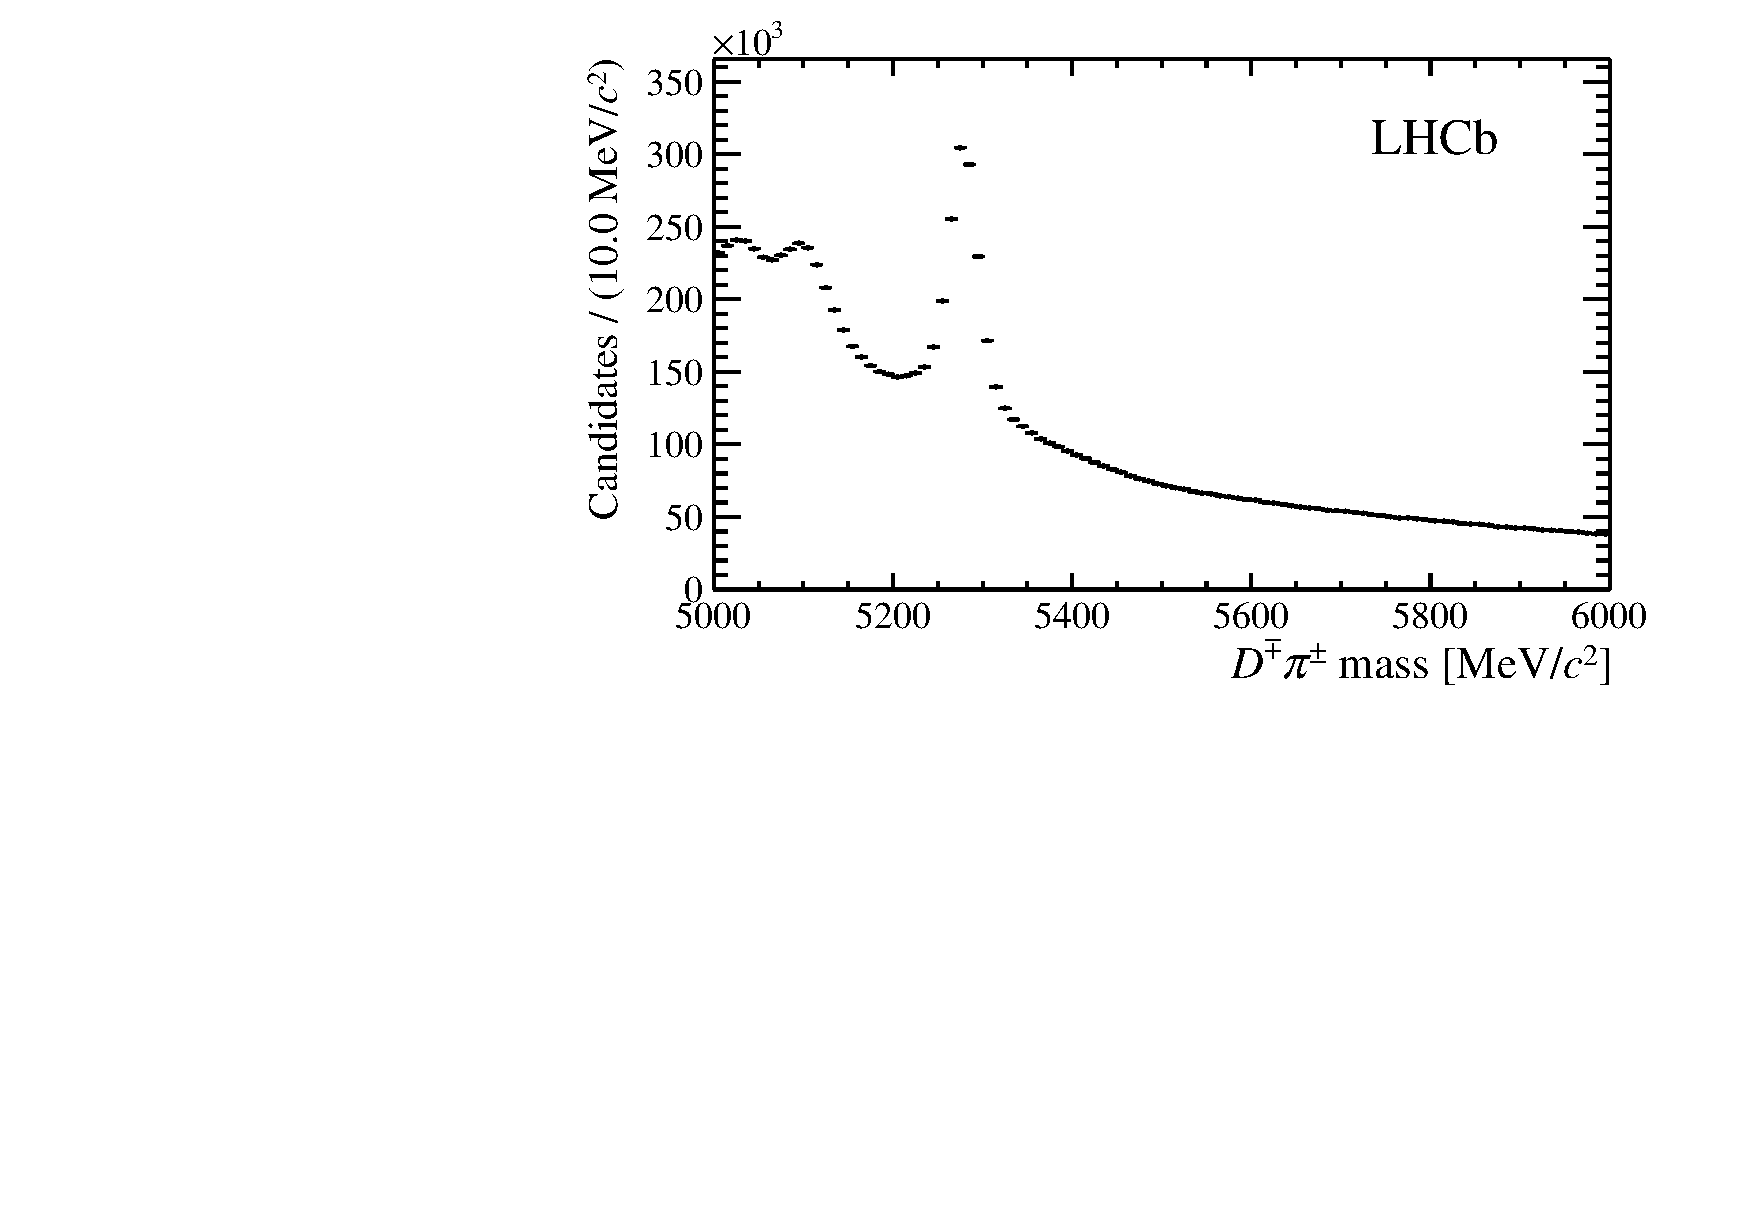
\includegraphics[width=0.49\textwidth]{06selection/figs/Bmass_afterStrippingAndTrigger.pdf}
    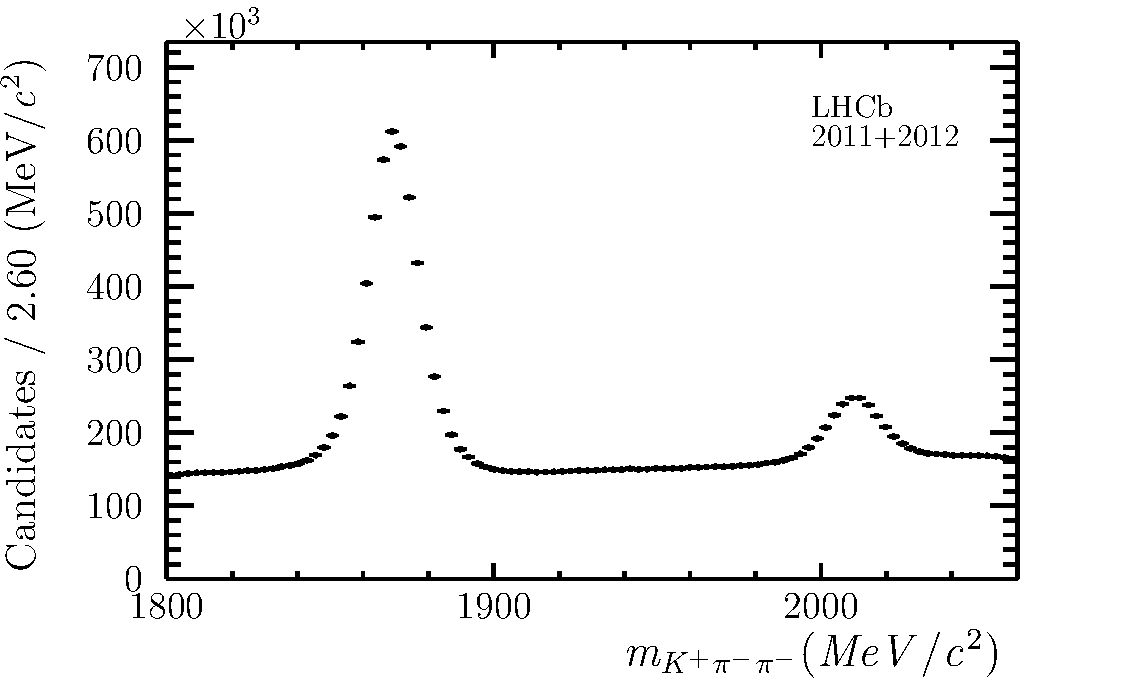
\includegraphics[width=0.49\textwidth]{06selection/figs/Dmass_afterStrippingAndTrigger.pdf}
    \caption{Invariant mass distributions of the $\Dm\pip$ combination using the DTF with a \Dm-mass constraint (right) and of the \Kp\pim\pim combination without any constraint (right).}
    \label{fig:BAndDmassAfterStripping}
\end{figure}
For this analysis no specifc requirements at the L0 level are made.
On the HLT1 level the \Bz candidates are required to be TOS on the \verb!Hlt1TrackAllL0Decision! line
In the HLT2 trigger stage the \BdToDpi candidates are required to be TOS on either the \verb!Hlt2Topo2BodyBBDTDecision! line, the \verb!Hlt2Topo3BodyBBDTDecision! line  or the \verb!Hlt2Topo4BodyBBDTDecision! line.
These lines require a \ac{SV} formed out of two, three or four tracks with a significant separation from the \ac{PV}~\cite{Trigger_Gligorov}.
In \cref{fig:BAndDmassAfterStripping} the invariant mass distributions of the \Bz and \Dm candidates are shown. The \Bz peak is clearly together with structures from the partially reconstructed decays $\Bz\!\to\Dm\rhop$ and $\Bz\!\to\Dstarm\pip$.
The distribution of the invariant mass of the \D-meson shows the \Dm peak at \SI[per-mode=symbol]{1870}{\MeVcc} and a \Dstarm peak at \SI[per-mode=symbol]{2010}{\MeVcc}.
After the trigger requirements some lose sanity cuts to remove clear background candidates are applied.
These cuts are listed in \cref{tab:preselection}.
\begin{table}[tbp]
	\centering
	\caption{Preselection cuts applied after the trigger requirements.}
	\begin{tabular}{cc}
		\toprule
		\multicolumn{2}{c}{\Dm daughter requirements}\\
		\midrule
		\dllkpi for pions	& $<8.0$ \\
		\dllkpi for kaons 	& $>-2.0$ \\
		\midrule
		\multicolumn{2}{c}{\Dm- and \Bz-meson requirements}\\
		\midrule
		$\left|m_{\Kp\pim\pim}-m_\Dm^{\text{PDG}}\right|$	& $<\SI[per-mode=symbol]{35}{\MeVcc}$ \\
		\Bz decay time										& $>\SI{0.2}{\pico\second}$ \\
		\bottomrule
	\end{tabular}
	\label{tab:preselection}
\end{table}

\subsection{Background vetoes}
\label{sec:vetoes}

Before a multivariate classifier is trained on and applied to a data sample, this should at best only consist of the candidates which are supposed be separated by the classifier.
In this case these candidates are \BdToDpi signal candidates and combinatorial background.
Therefore backgrounds due to kinematic failures in the reconstruction and wrong associations between a \Bz candidate and a \ac{PV} are vetoed.

\subsubsection*{Mass vetoes}

First, the investigated sources of backgrounds which arise due to failures in the reconstrucion, and if necessary, the applied vetoes are described.
Such failures can be missed neutral particles or misidentified particles in the reconstruction.

The first type of backgrounds arises from the decay $\Bz\!\to\Dm\mup\neum$. When missing the neutrino and misidentifying the muon as a pion this decay would falsely be reconstructed as the signal decay \BdToDpi.
This is vetoed with a binary requirement on the bachelor particle not to be a muon.
This binary requirement is based on the number and the region of the muon stations where hits are found and the momentum of the track~\cite{Archilli:2013npa}.

The following kinematic backgrounds are all due to misidentification of particles in the finalstate.
Misidentification between protons and pions can lead to backgrounds from $\Lb\!\to\Lcbar\pip$ decays where the \Lcbar decays into a kaon, a pion and an antiproton.
To identify such background candidates a proton-mass hypothesis is applied to both daughter pions of the \Dm-meson.
After combining the three \D daughters again a peak around the \Lc mass becomes visible in the distributions shown in \cref{fig:LcVeto}.
The distributions look different, because of the pions, which are originally sorted by transverse momentum \pt.
\begin{figure}[tbp]
    \centering
    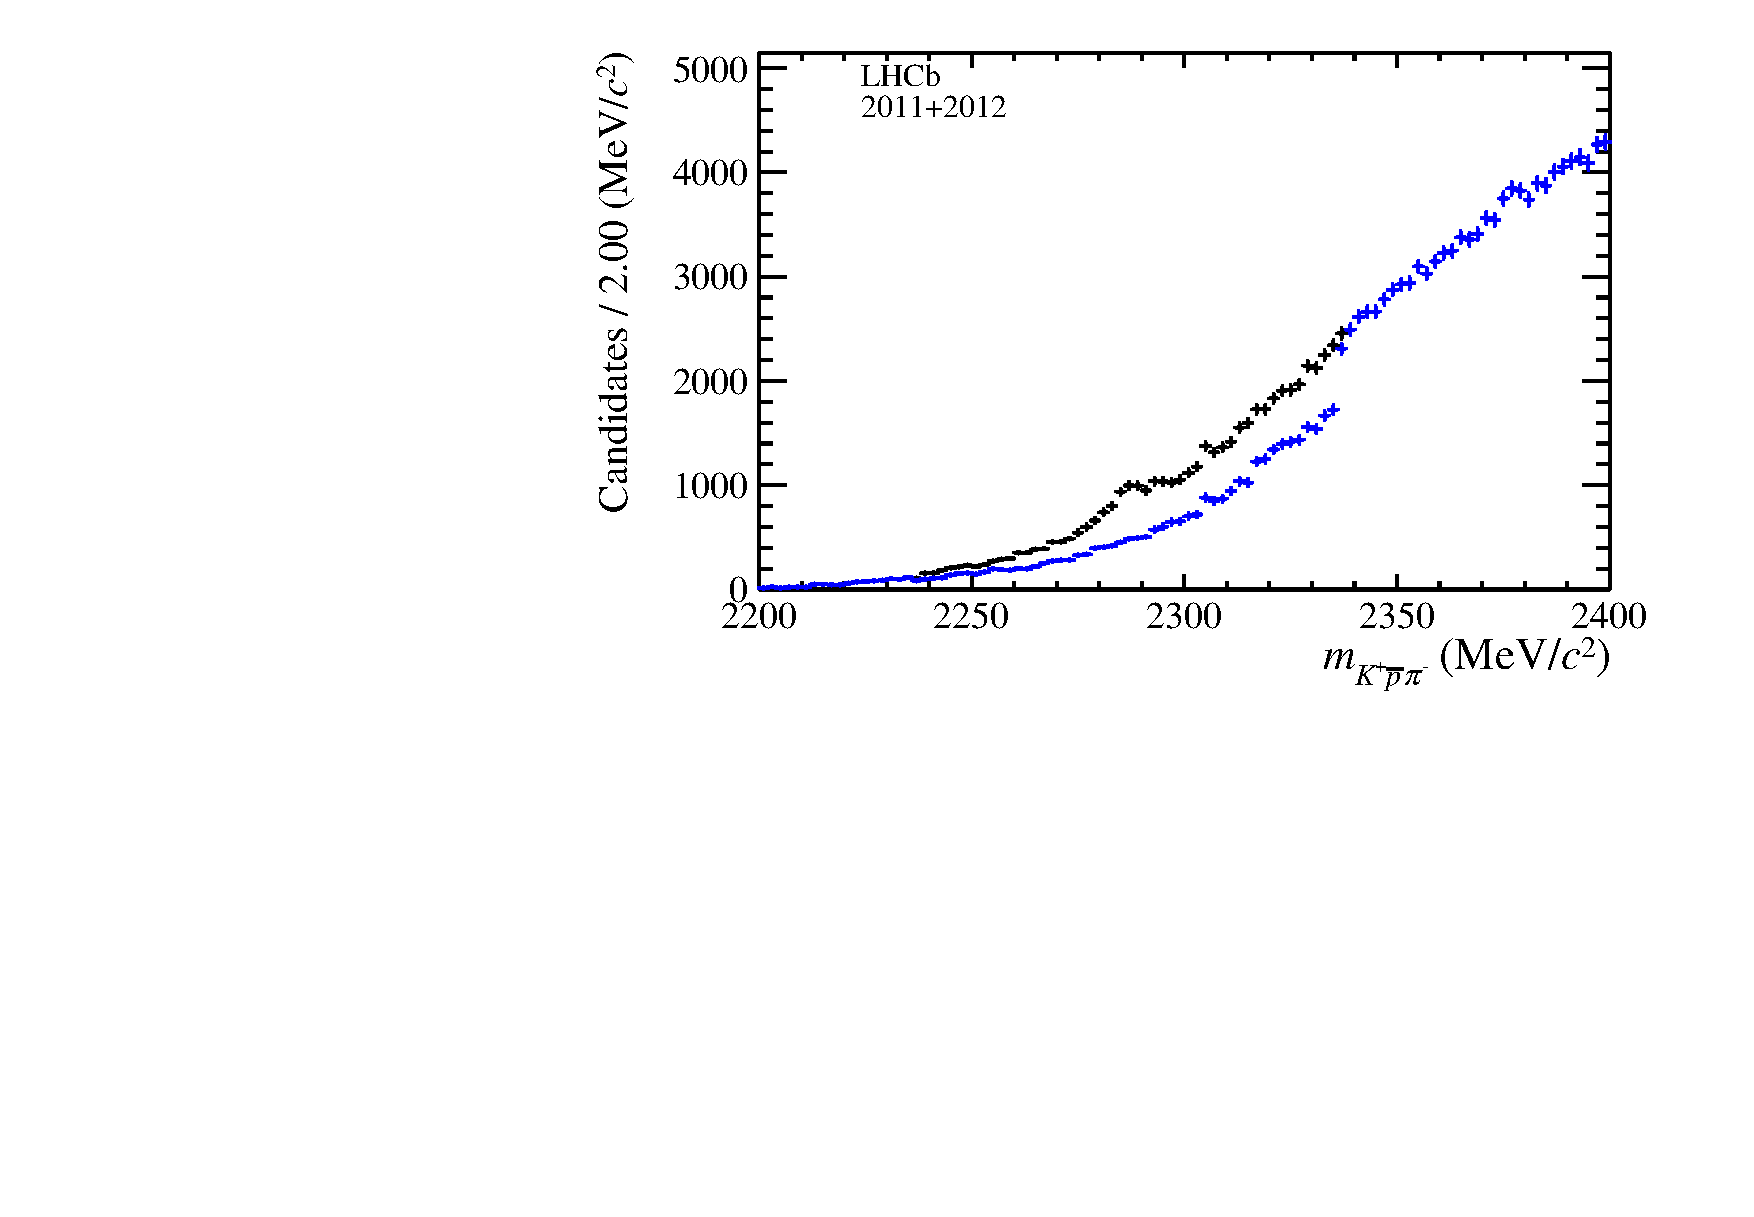
\includegraphics[width=0.49\textwidth]{06selection/figs/LcHypo1.pdf}
    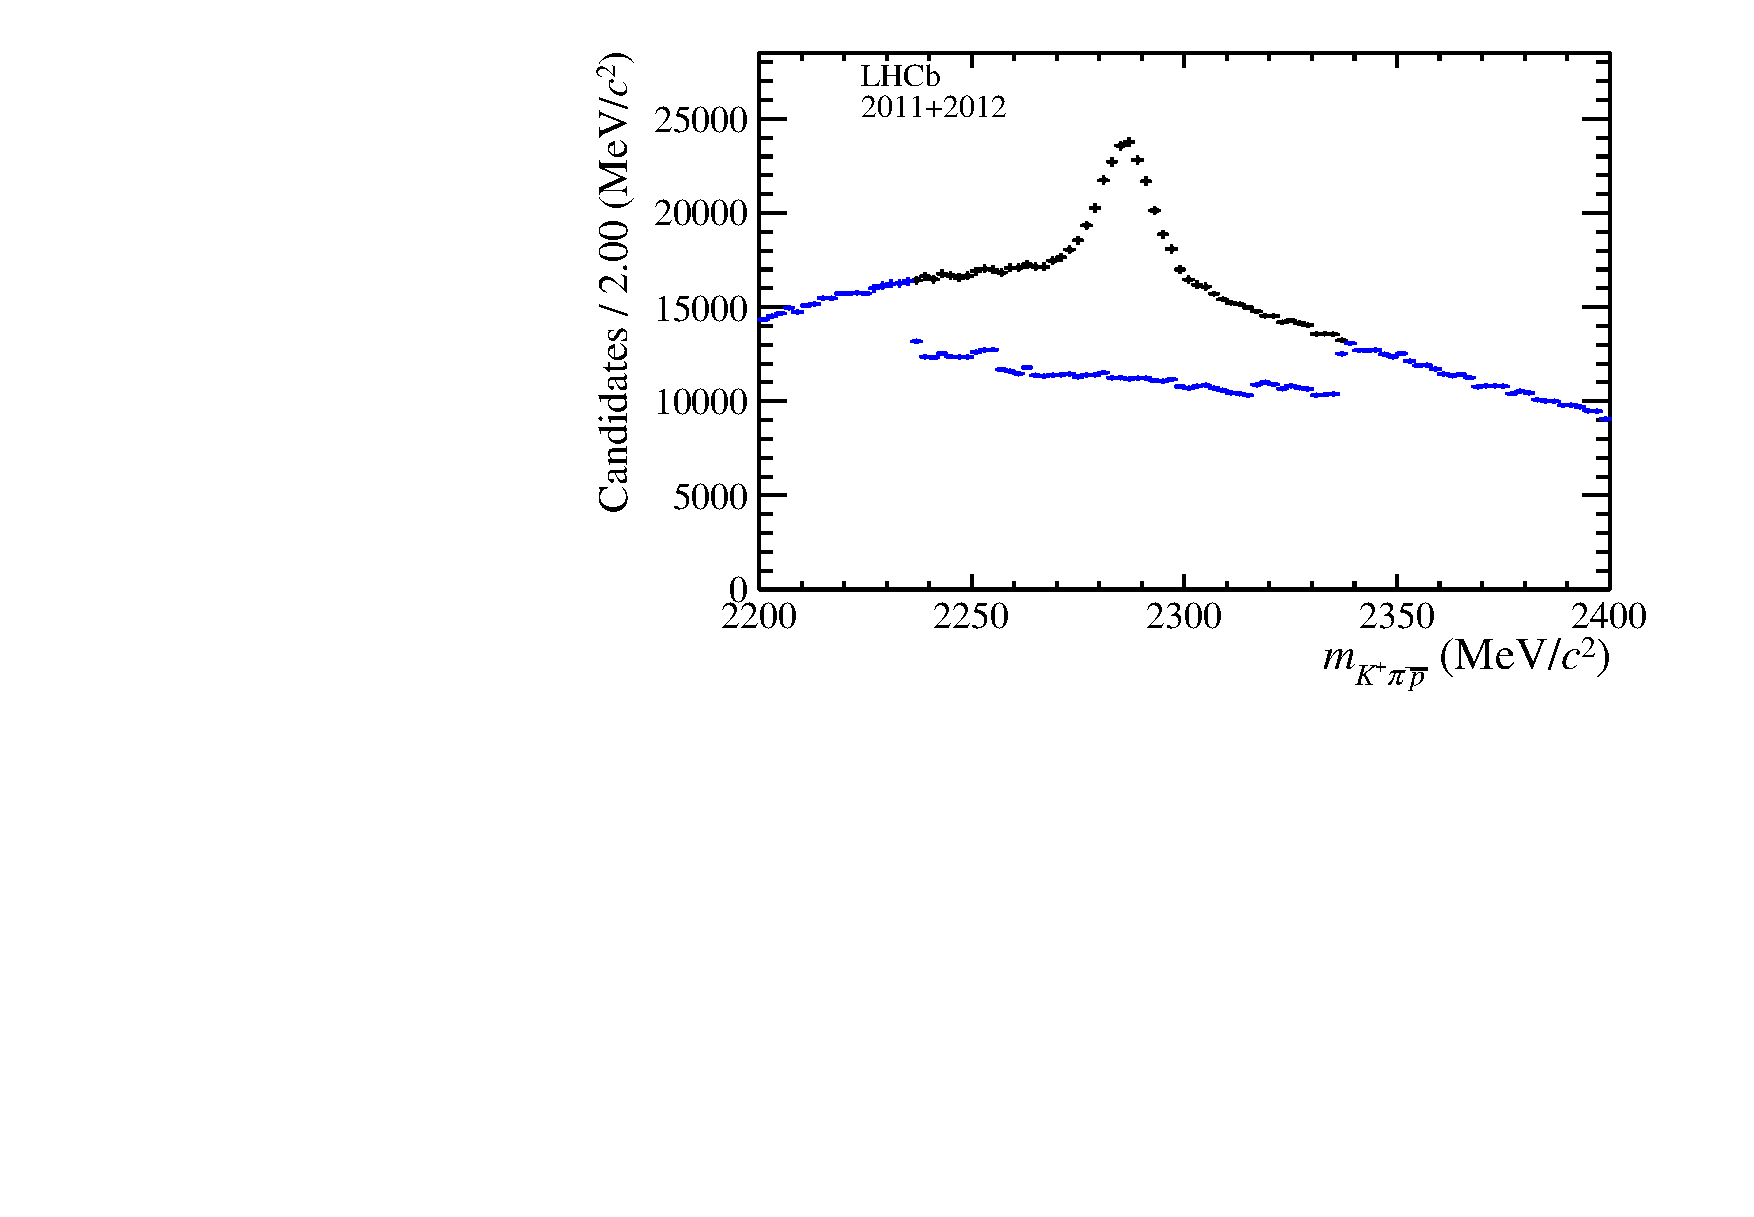
\includegraphics[width=0.49\textwidth]{06selection/figs/LcHypo2.pdf}
    \caption{Invariant mass distributions of the $\kaon\pion\proton$ combinations for both daughter pions of the \Dm-meson.
    The distributions are shown without the veto (black) and with the veto applied (blue).
    The left (right) plot shows the proton-mass hypothesis applied to the pion with lower (higher) transverse momentum.}
    \label{fig:LcVeto}
\end{figure}
To remove this background a two-stage veto is applied: In the first stage candidates are rejected if the invariant mass of the three hadrons is inside a \SI[per-mode=symbol]{30}{\MeVcc}  window around the nominal \mbox{\Lcbar-mass} $m_\Lcbar^{\text{PDG}}=\SI[per-mode=symbol]{2286.46}{\MeVcc}$ and the \dllppi is larger than \num{-8.0}.
In the second stage the mass window is enlarged to \SI[per-mode=symbol]{30}{\MeVcc} around the nominal \Lcbar-mass, but the \dllppi is loosened, only requiring $\dllppi>-5.0$.
After the preselection already \SI{99.720\pm0.004}{\percent} of the $\Lb\!\to\Lcbar\pip$ candidates are rejected.
This veto rejects another \SI{76.6\pm0.6}{\percent} at a signal efficiency of \SI{93.48\pm0.06}{\percent}.

In the same way as pions and protons can be misidentified it can happen that a kaon is falsely identified as one of the \Dm daughter pions.
Such misidentification gives rise to a potential background contamination from $\Bs\!\to\Dsm\pip$ candidates.
As before, for both pions a kaon mass hypothesis is applied and the three \Dm-daughters are combined.
However,  these distributions do not show a clear mass peak.
Therefore they are compared for different kinematic regions of the invariant $\left[\Kp\pim\pim\right]\pip$ mass: After applying the kaon mass hypothesis, $\Bs\!\to\Dsm\pip$ candidates should end up in the \Bs signal region, whereas no $\Bs\!\to\Dsm\pip$ candidates are expected in the upper-mass sideband $m_{\left[\Kp\pim\pim\right]\pip}>\SI[per-mode=symbol]{5500}{\MeVcc}$.
Therefore the invariant mass distributions of the \kaon\kaon\pion system are compared for candidates from the \Bs signal range \SIrange[per-mode=symbol]{5330}{5400}{\MeVcc} and a background range \SIrange[per-mode=symbol]{5500}{5700}{\MeVcc}.
The visible difference in \cref{fig:DsVeto} stems from the fact that those two distributions arise from different kinematic regions.
\begin{figure}[tbp]
    \centering
    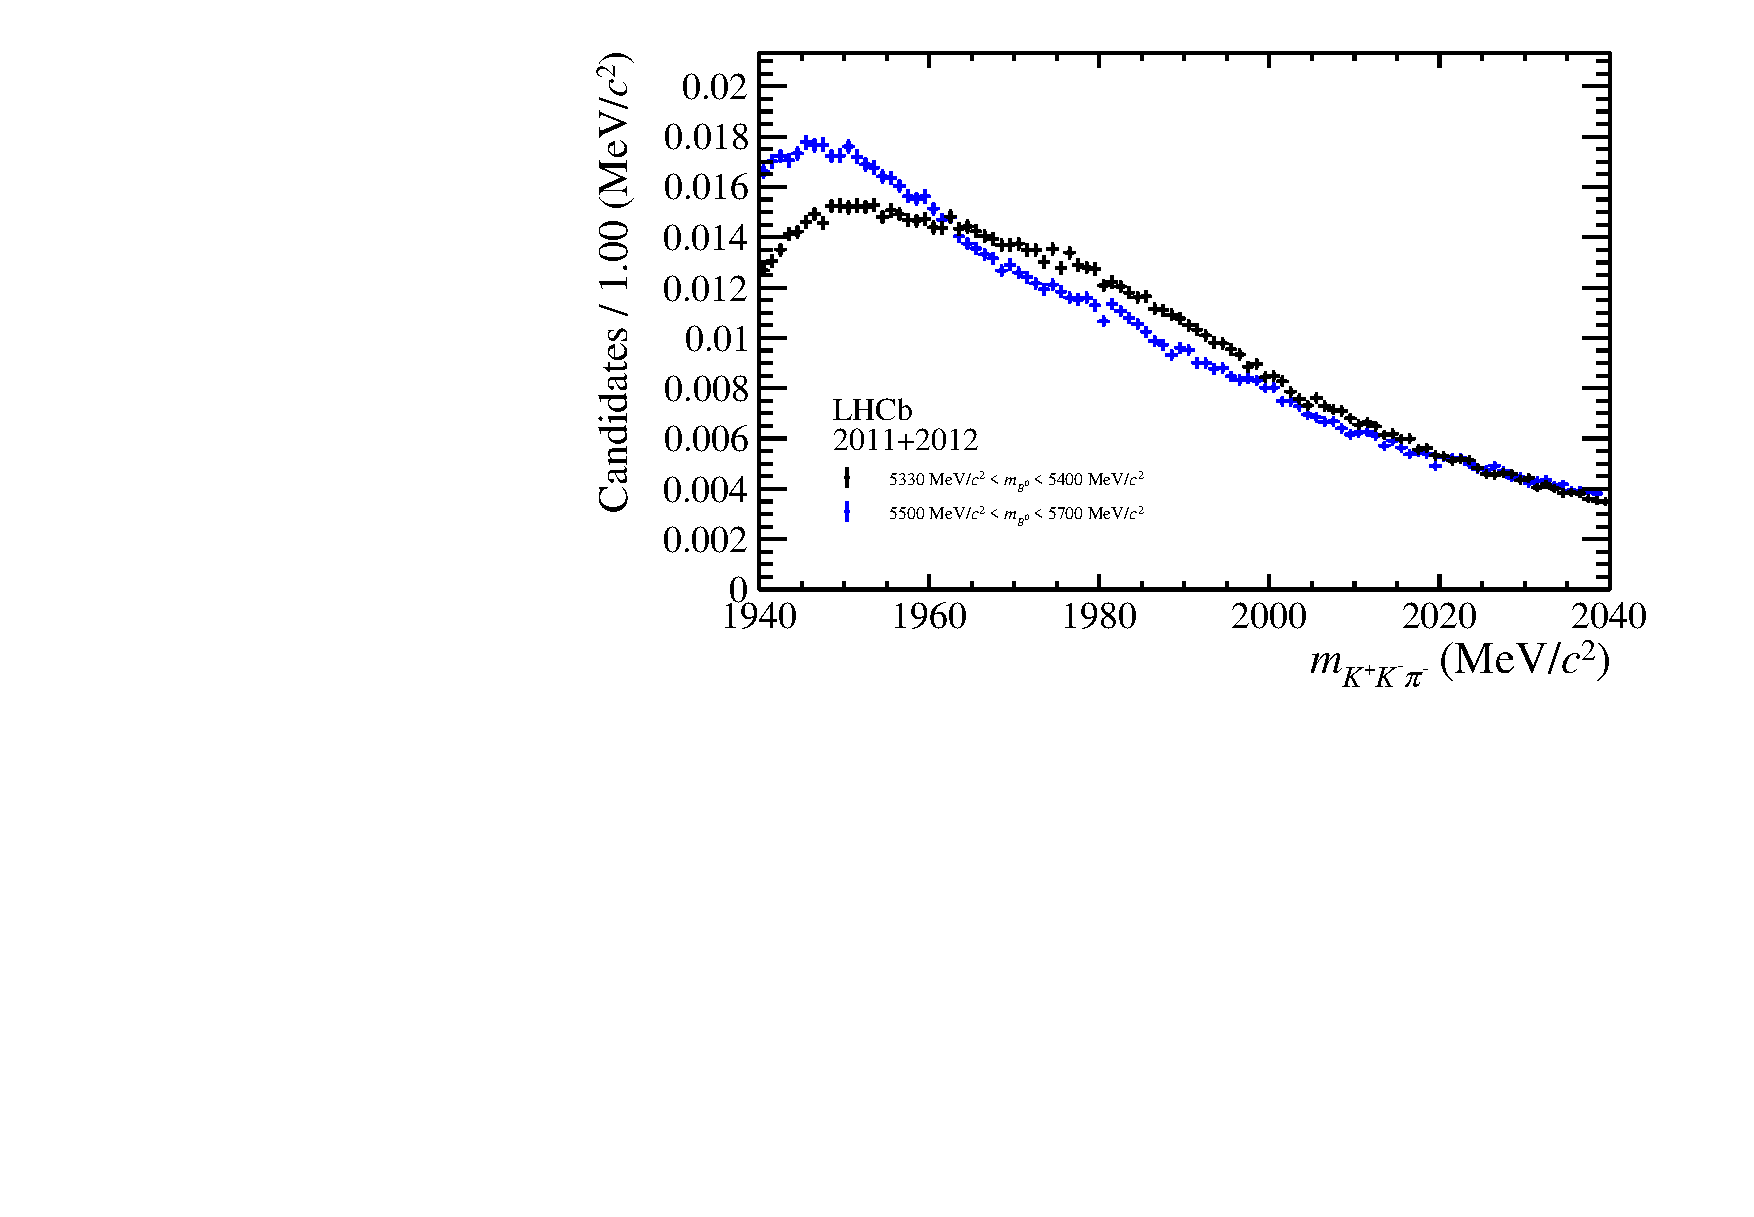
\includegraphics[width=0.49\textwidth]{06selection/figs/DsHypo1.pdf}
    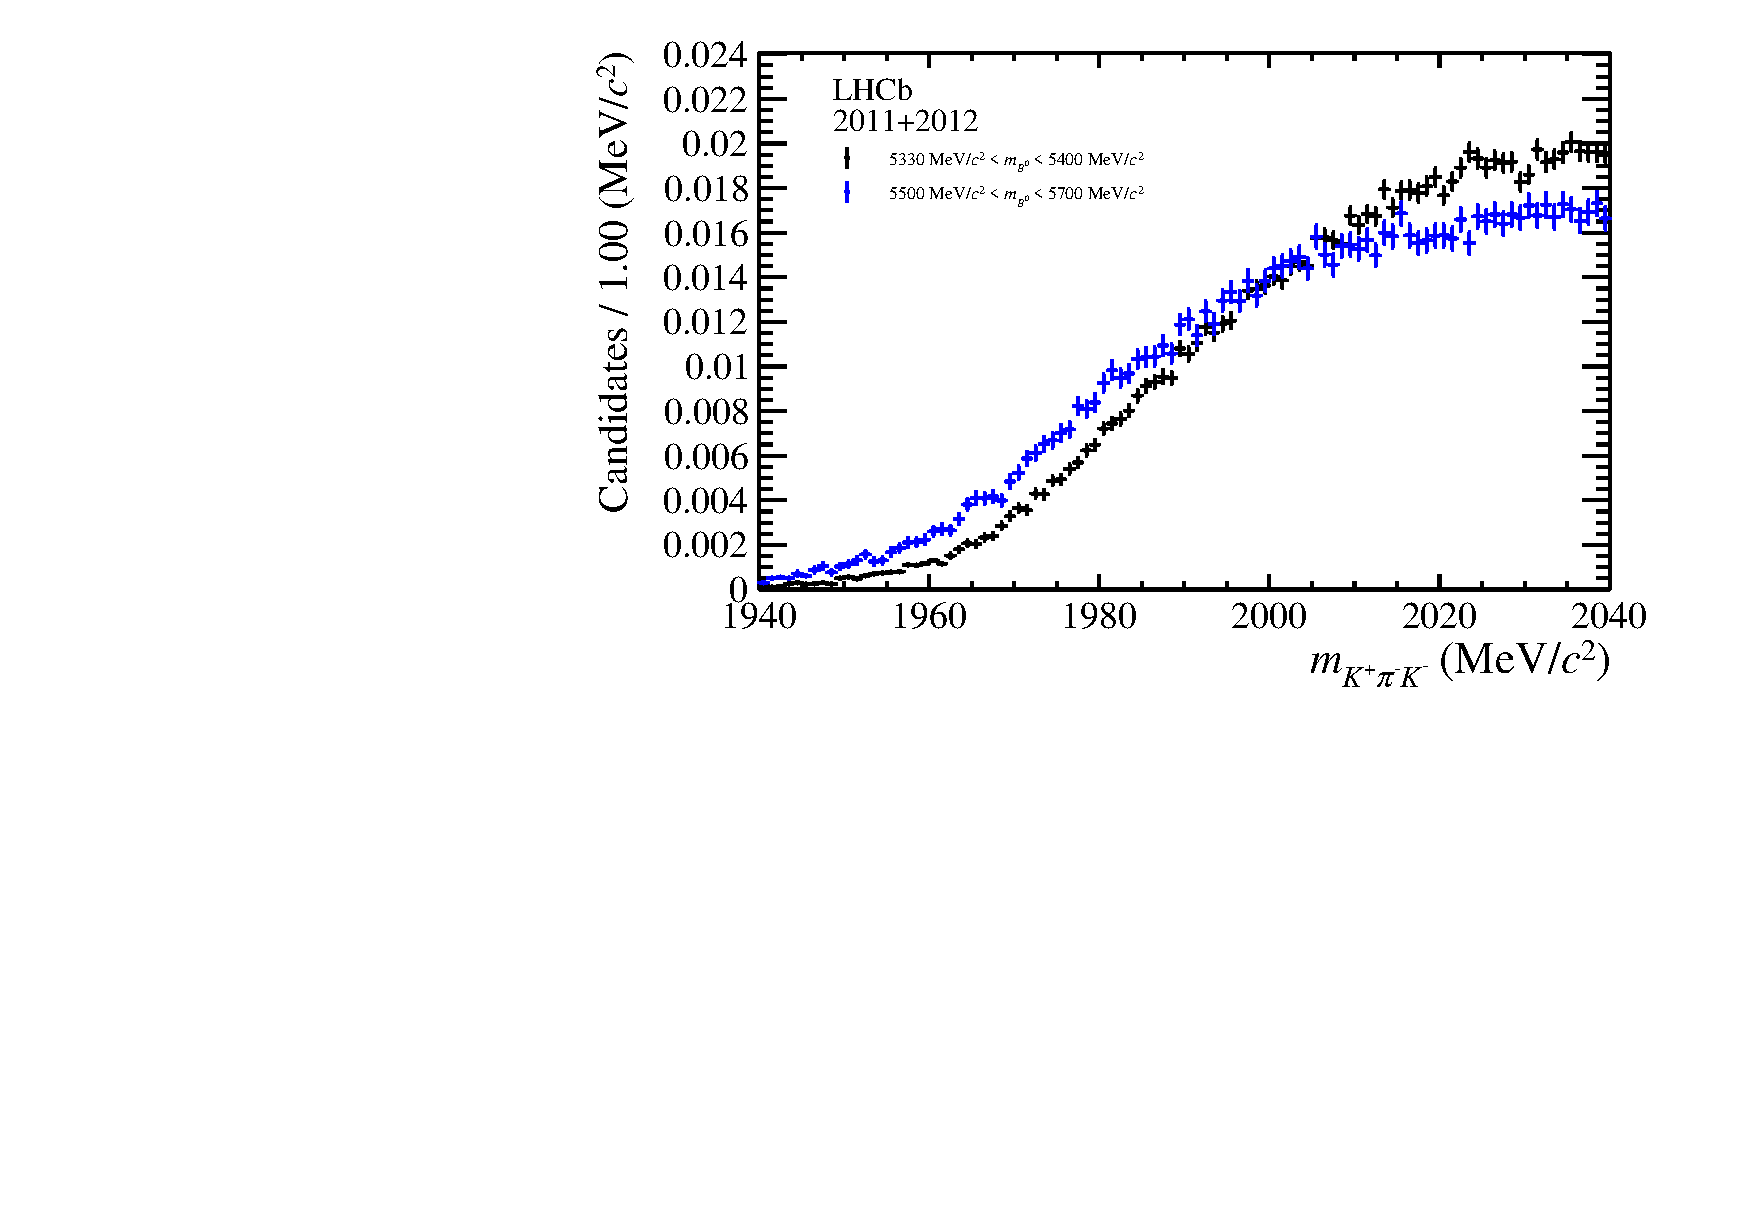
\includegraphics[width=0.49\textwidth]{06selection/figs/DsHypo2.pdf}
    \caption{Invariant mass distributions of the $\kaon\kaon\pion$ combinations for both daughter pions of the \Dm-meson.
    After applying the kaon mass hypothesis the distributions are shown in the \Bs signal region from \SIrange[per-mode=symbol]{5330}{5400}{\MeVcc} (black) and in a background region from \SIrange[per-mode=symbol]{5500}{5700}{\MeVcc} (blue).
    In the left plot the kaon-mass hypothesis is applied to the pion with lower transverse momentum, right to the pion with higher transverse momentum.}
    \label{fig:DsVeto}
\end{figure}
To further ensure that no significant contamination from $\Bs\!\to\Dsm\pip$ candidates is present in the data, resonances like \Kstarz- or $\phi$-mesons, which arise in possible \Dsm decays are studied.
Those resonances would become visible in the \kaon\kaon ($\phi$) and \kaon\pion (\Kstarz) invariant mass distributions.
Figure \ref{fig:phi_Kst_veto} shows exemplary the invariant mass distributions of the \kaon\kaon (\kaon\pion) combinations of the the daughter kaon with the
pion with larger transverse momentum under the kaon mass hypothesis (under the initial pion mass hypothesis).
Additionally to the beforehand defined signal and background regions only candidates within a range from \SIrange[per-mode=symbol]{1940}{2040}{\MeVcc} from \cref{fig:DsVeto} are considered for these plots.
Consequently in the signal region a peaking structure would be expected in case of a significant contamination with $\Bs\!\to\Dsm\pip$ decays.
As no distribution in \cref{fig:DsVeto} and \cref{fig:phi_Kst_veto} shows such structure, background candidates from $\Bs\!\to\Dsm\pip$ decays are assumed to be negligible.
\begin{figure}[tbp]
    \centering
    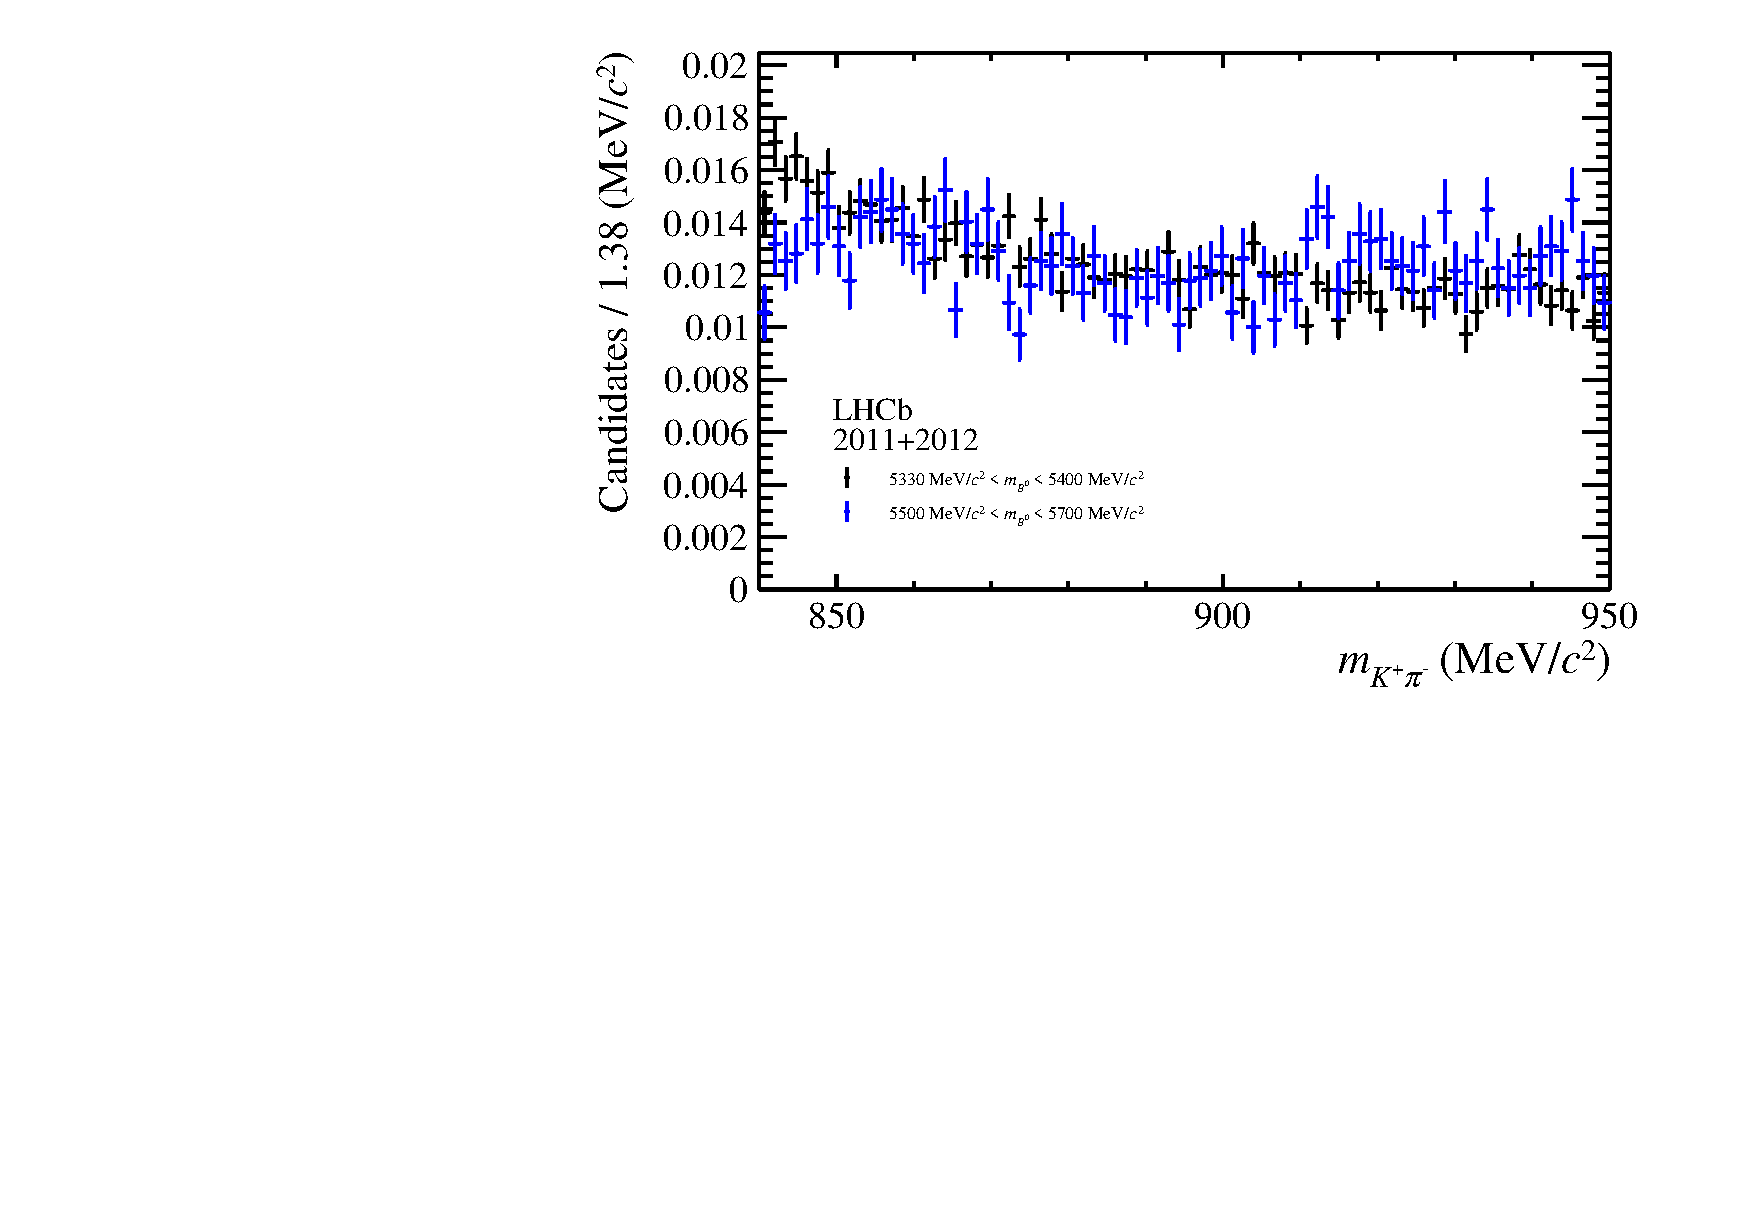
\includegraphics[width=0.49\textwidth]{06selection/figs/KstarHypo2.pdf}
    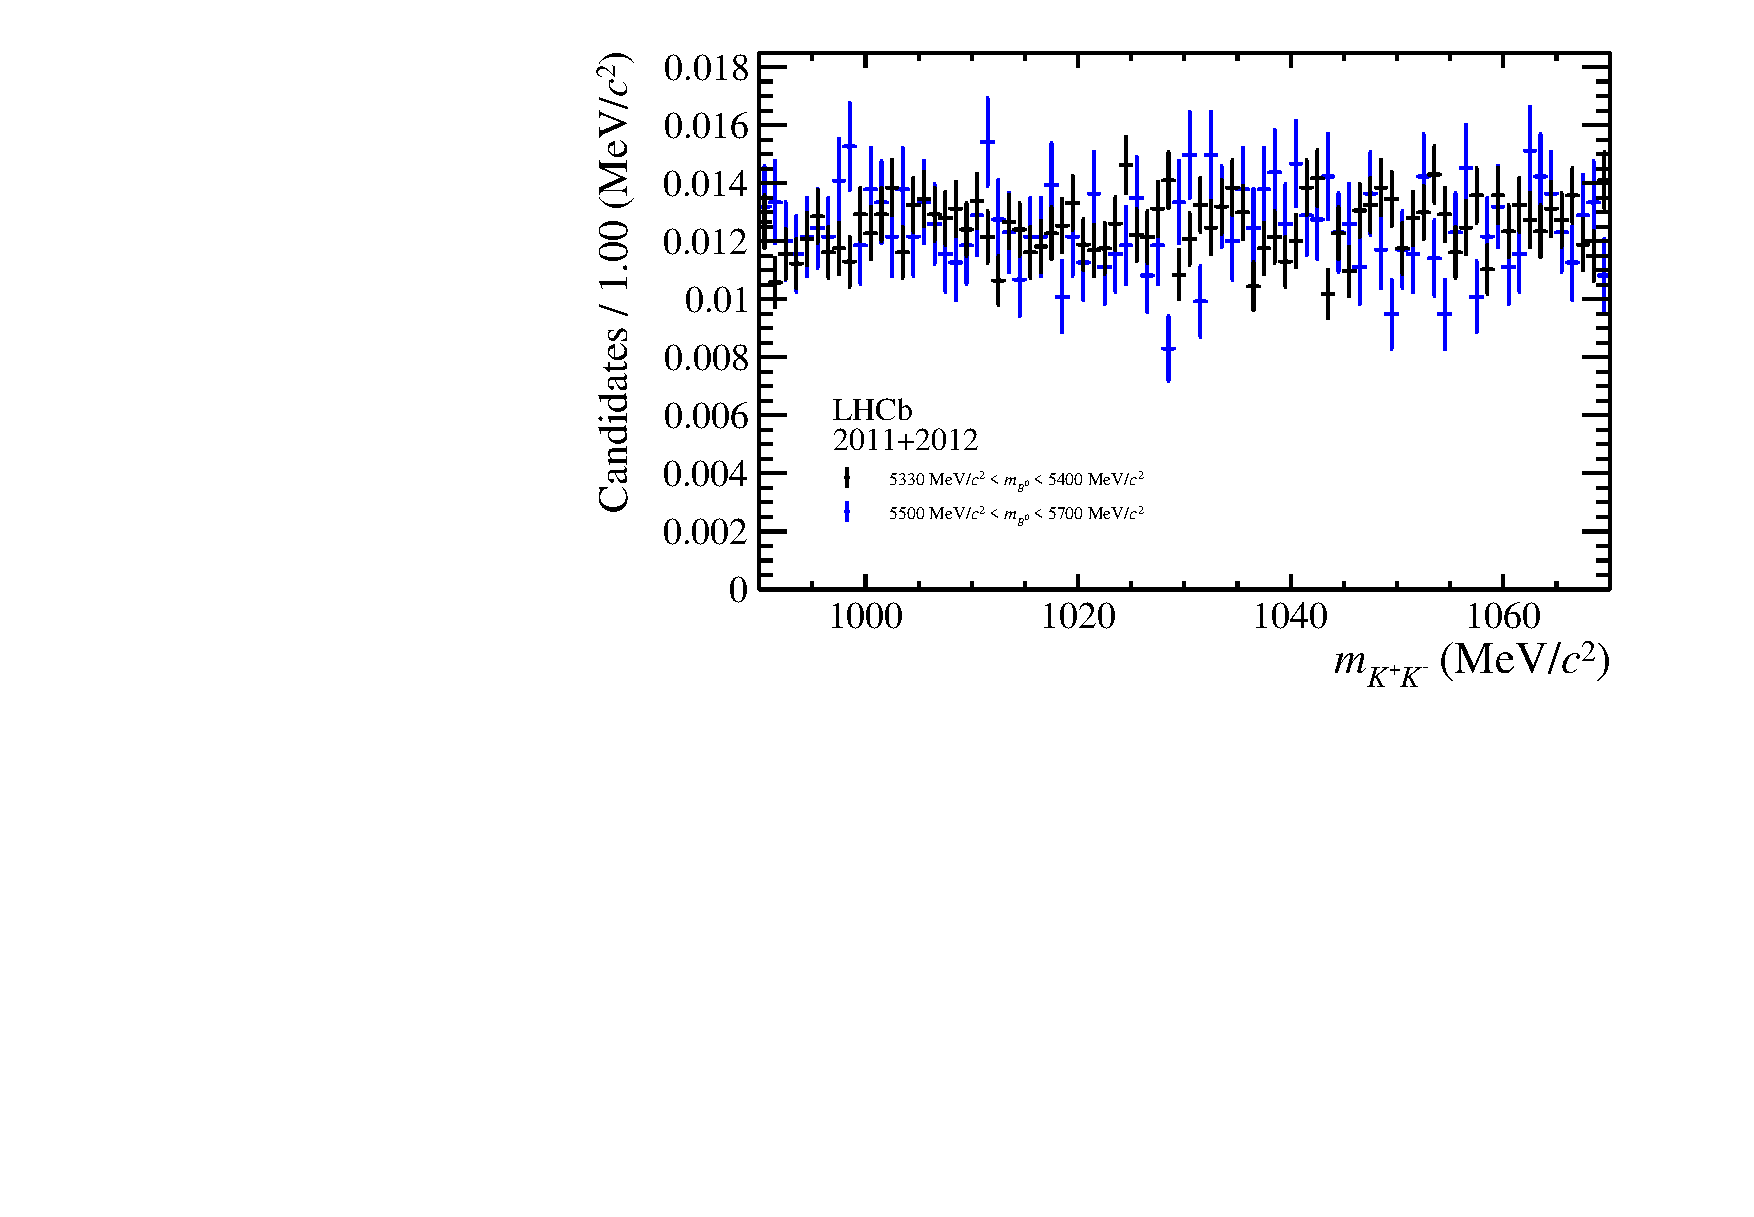
\includegraphics[width=0.49\textwidth]{06selection/figs/PhiHypo2.pdf}
    \caption{Invariant mass distributions of the \kaon\pion (left) and \kaon\kaon (right) combinations for the daughter pion of the \Dm-meson with larger transverse momentum with the daughter kaon or remaining daughter pion, respectively.
    Only candidates with $\SI[per-mode=symbol]{1940}{\MeVcc}<m_{\kaon\kaon\pion}<\SI[per-mode=symbol]{2040}{\MeVcc}$ are considered.
    The invariant mass distributions are shown in the in the \Bs signal region from \SIrange[per-mode=symbol]{5330}{5400}{\MeVcc} (black) and in a background region from \SIrange[per-mode=symbol]{5500}{5700}{\MeVcc} (blue).}
    \label{fig:phi_Kst_veto}
\end{figure}

The last background comes from $\Bz\!\to\DorDbar\kaon\pion$ decays, arising due to a kaon-pion misidentification of the bachelor track or a \Dm-daughter track, followed by a combination the bachelor track with a \Dm-daughter particle.
When doing the four possible combinations of applying the kaon hypothesis to the bachelor particle and the two \Dm-daughter pions all distributions show a flat shape.
Hence, backgrounds from $\Bz\!\to\DorDbar{}^0\kaon\pion$ decays are assumed to be negligible.
In \cref{fig:DzVeto} the combinations of the bachelor track with the \Dm-daughter pion with higher transverse momentum are shown for illustration.
\begin{figure}[tbp]
    \centering
    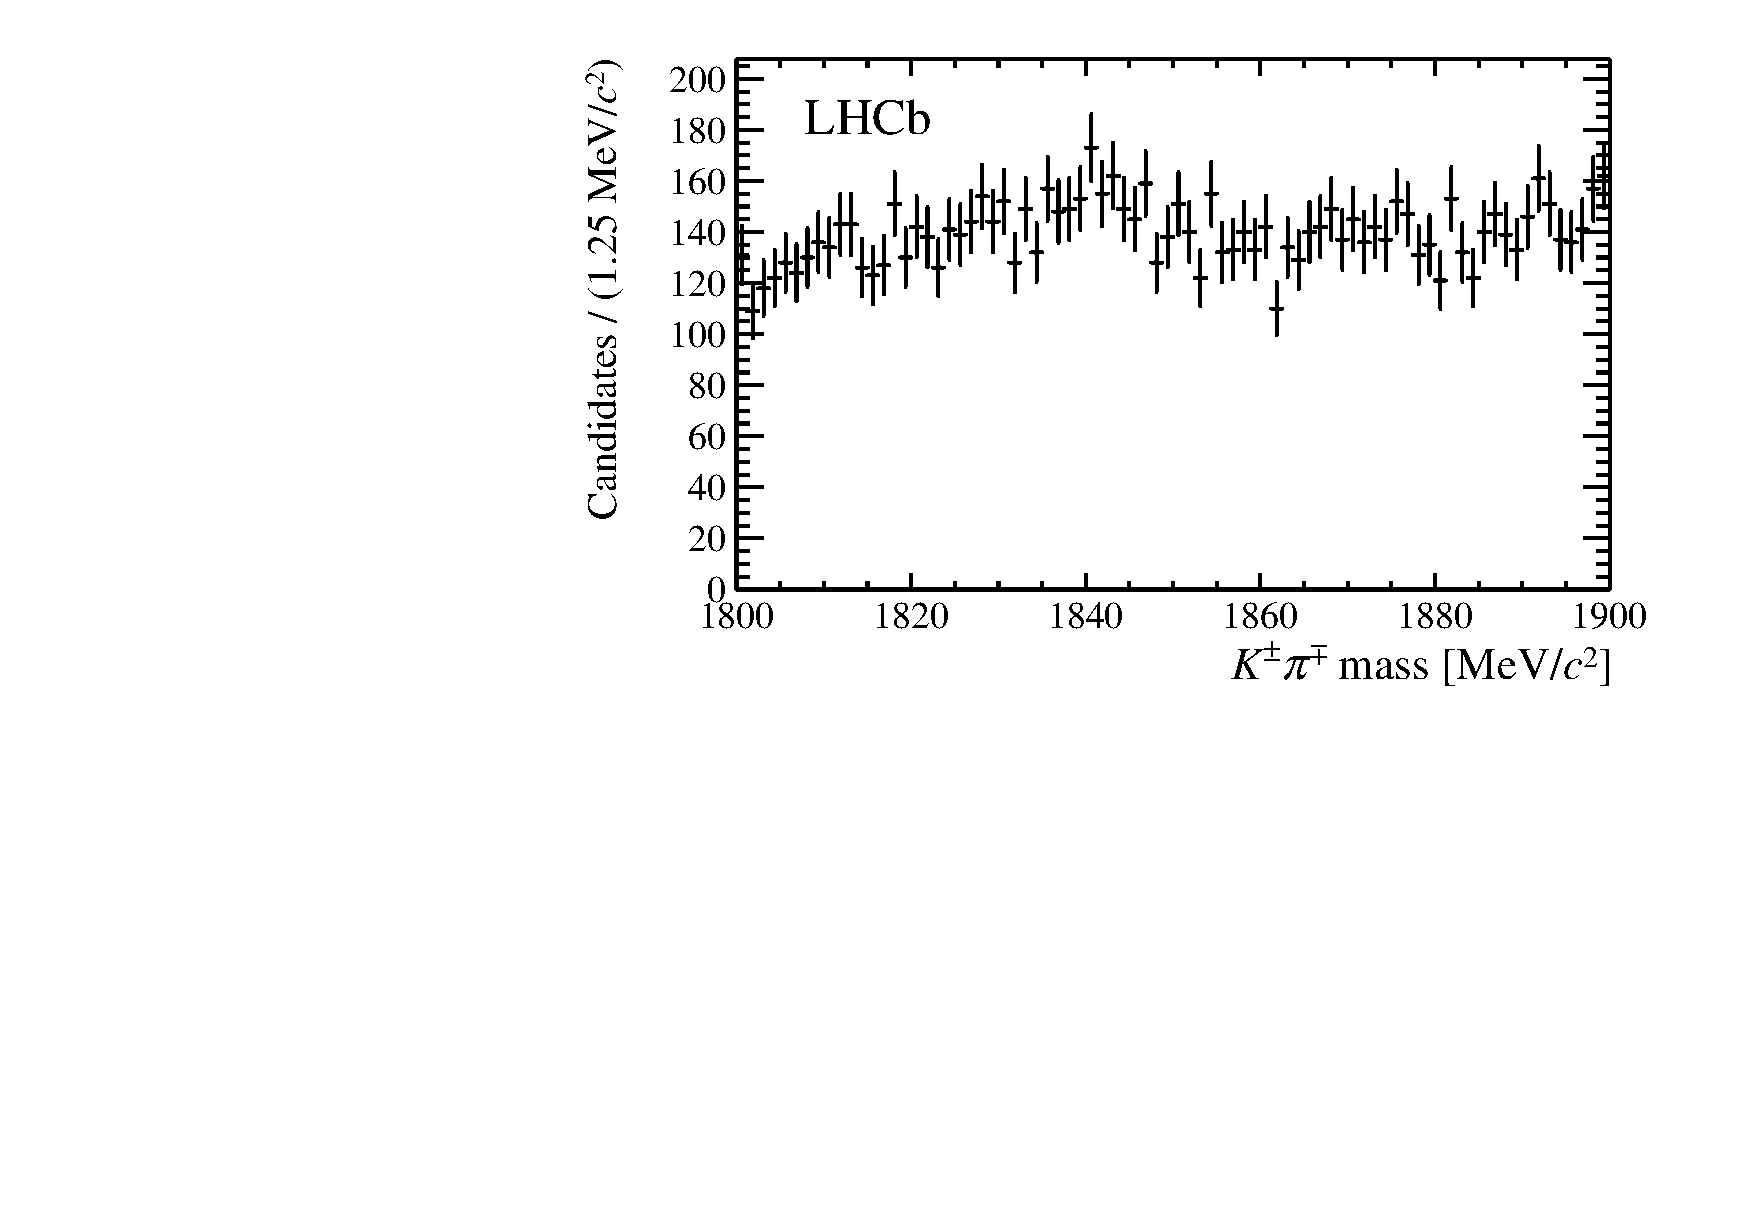
\includegraphics[width=0.49\textwidth]{06selection/figs/D0Hypo3.pdf}
    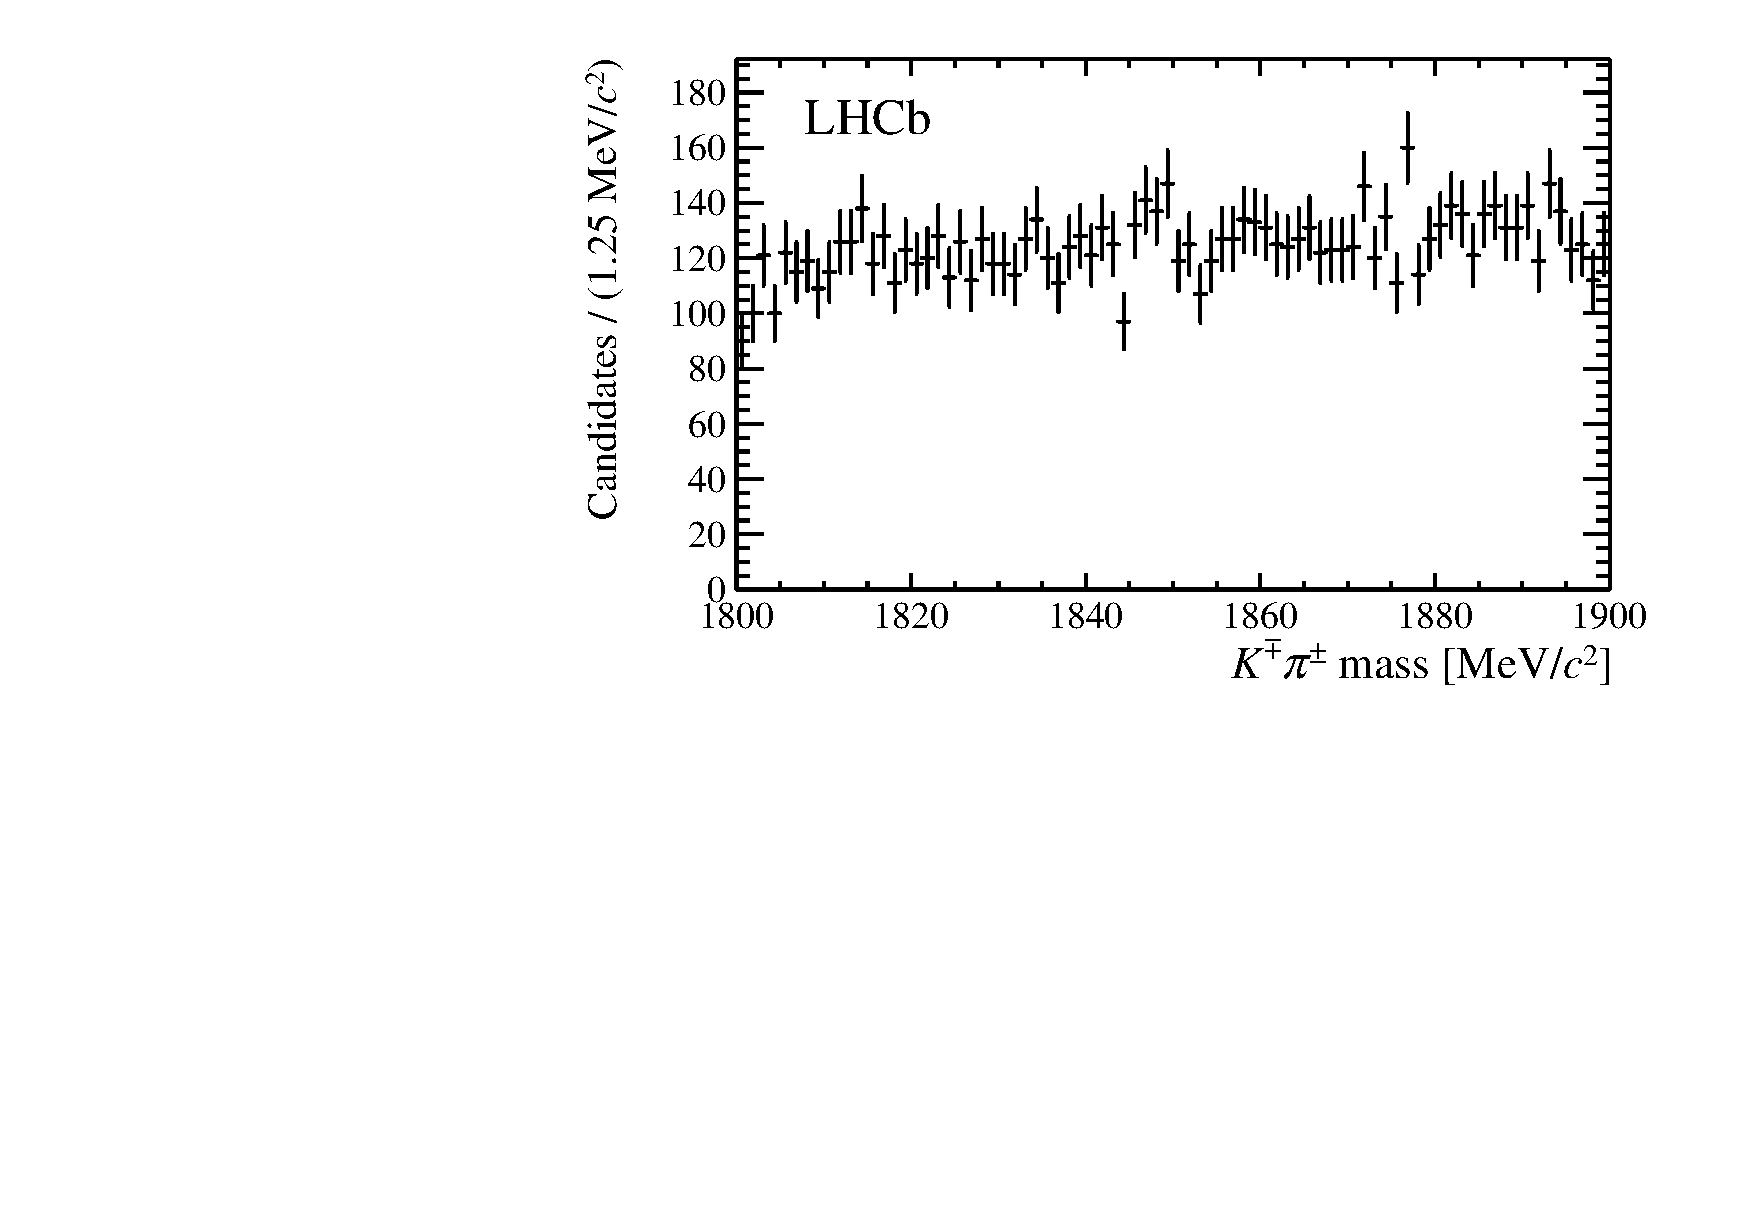
\includegraphics[width=0.49\textwidth]{06selection/figs/D0Hypo4.pdf}
    \caption{Invariant mass distributions for the combinations of the bachelor particle with the \Dm-daughter pion with higher transverse momentum.
    In the left plot the kaon hypothesis is applied to the bachelor pion, the right plot shows the kaon hypothesis applied to the \Dm-daughter pion.}
    \label{fig:DzVeto}
\end{figure}

\subsubsection*{Wrongly associated PVs}

The average number of \proton\proton-collisions per bunch crossing is $\nu=2.5$.
Therefore a considerable amount of events has more than one \ac{PV} and in these events a \Bz candidate can be associated with each of them.
Besides that an event can also contain more than one \Bz candidate; in this case the \Bz candidate is chosen randomly (more details in \cref{sec:MultCands}).
However, in case of multiple \ac{PV}s per event the \Bz candidate can be associated with the wrong PV what leads to a wrong decay time for this candidate.
Usually a decay time dependent selection efficiency is expected at \lhcb, which strongly increases at small decay times up to $\approx\SI{2}{\pico\second}$ and shows a flat or slightly dropping distribution for high decay times.
This efficiency, further denoted as decay time acceptance, is caused by the track reconstruction in the \velo and certain trigger requirements (more details are given in \cref{sec:acceptance}).
Yet, due to the wrong \ac{PV} association a large, unexpected tail at high decay times arises.
This can be checked on simulation, where the true decay time is known.
Weighting each (\Bz,\ac{PV})-candidate with an exponential using the true lifetime of the \Bz candidates - \ie (\Bz,\ac{PV})-candidates with high decay times get higher weights - shows an excess of (\Bz,\ac{PV})-candidates at high decay times (see \cref{fig:WrongPVMC}).
\begin{figure}[tbp]
    \centering
    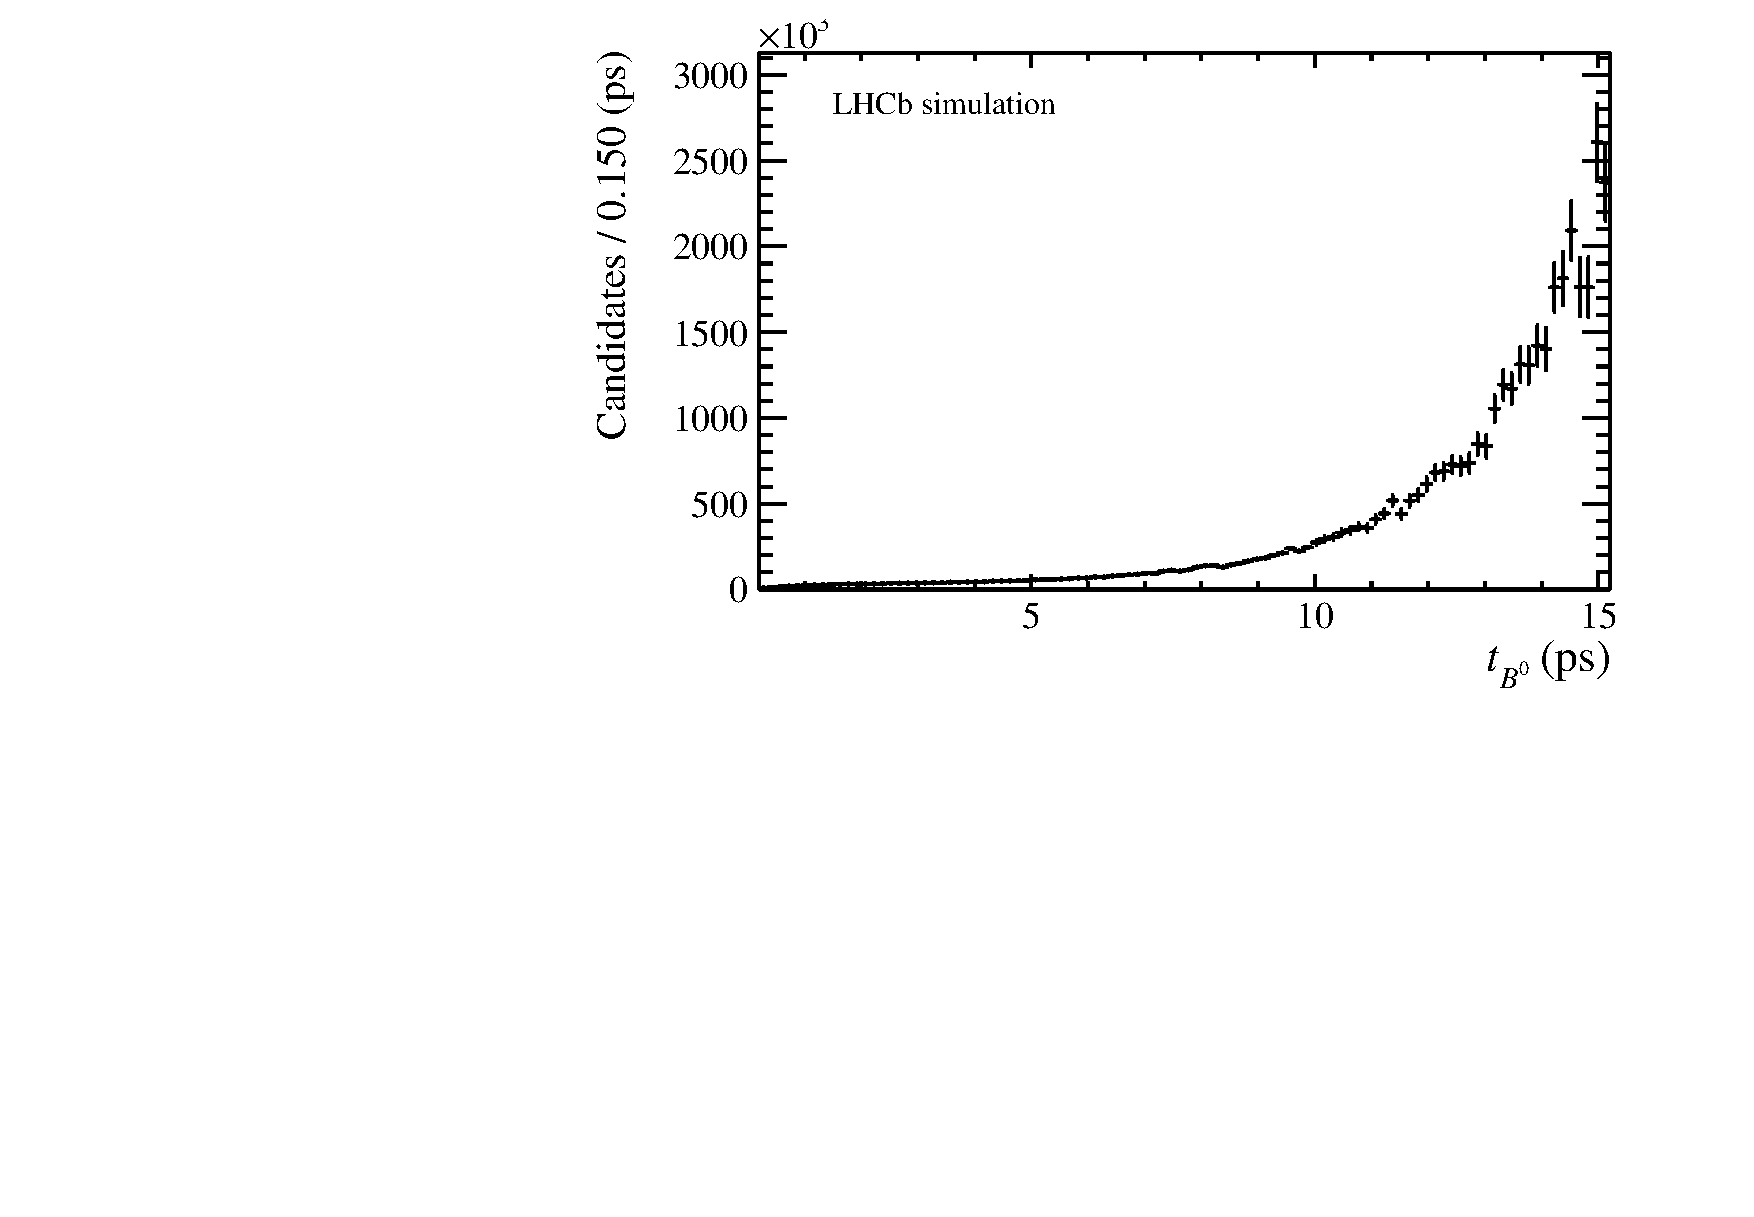
\includegraphics[width=0.45\textwidth]{06selection/figs/WrongPVs-weightedBad.pdf}
    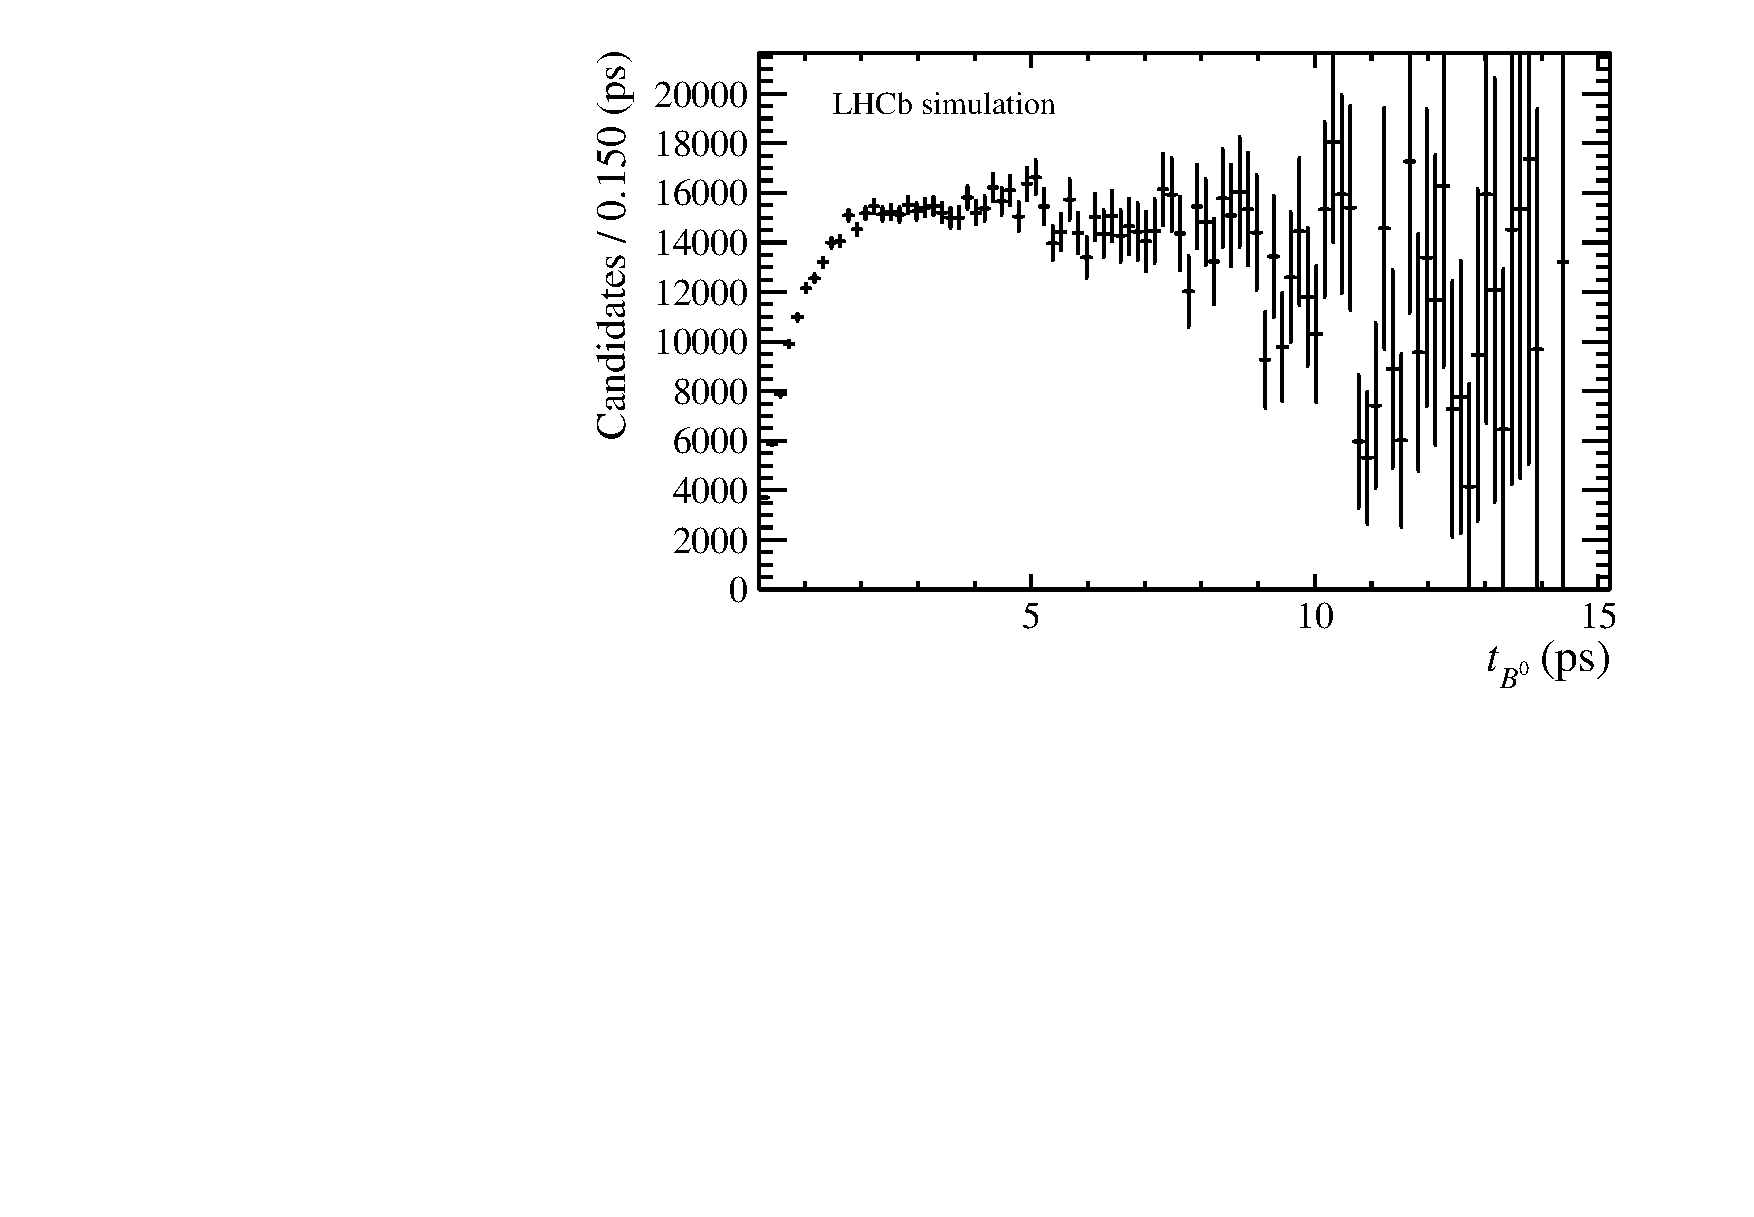
\includegraphics[width=0.45\textwidth]{06selection/figs/WrongPVs-weightedGoodMC.pdf}
    \caption{Left: Decay time distribution of simulated \BdToDpi candidates, wheighted with an exponential using the true lifetime of the \Bz candidates.
    At high decay times an excess of (\Bz,\ac{PV})-candidates can be seen.
    Right: Decay time distribution of simulated \BdToDpi candidates, wheighted with an exponential using the true lifetime of the \Bz candidates after applying a cut on the distance between the true and the reconstructed $z$ position of the \ac{PV}.
    The expected acceptance distribution at \lhcb is visible.}
    \label{fig:WrongPVMC}
\end{figure}
Further on simulation the true $z$-position of the \ac{PV} is known and can be compared with the reconstructed $z$-position.
Requiring that the distance between the true $z$-position of the \ac{PV} and the reconstructed $z$-position does not exceed five times the uncertainty on the reconstructed $z$-position removes the wrong associated (\Bz,\ac{PV})-candidates from the sample and the expected decay time acceptance becomes visible (\cref{fig:WrongPVMC}).
Though, this approach cannot be applied to data.
Therefore a criterion is developed requiring for each (\Bz,\ac{PV})-candidate the impact parameter $\chi^2_{\text{DTF,PV}}$ with any other \ac{PV} in the event ($\text{MinIP}\chi^2$) to be larger than a certain value.
This means that in case this $\text{MinIP}\chi^2$ is too small, the two corresponding \ac{PV}s cannot be distinguished sufficiently well from each other, and the (\Bz,\ac{PV})-candidate is rejected.
Events which contain just one \ac{PV} are kept always.
The cut is optimised in such a way, that \SI{98}{\percent} of the events in the simulated \BdToDpi sample are retained.
In \cref{fig:WrongPVData} the distribution of the $\text{MinIP}\chi^2$ variable together with the cut point at \num{16.5} and the resulting decay-time-acceptance distribution after applying the \enquote{data} criterion on simulation is shown.
\begin{figure}[tbp]
    \centering
    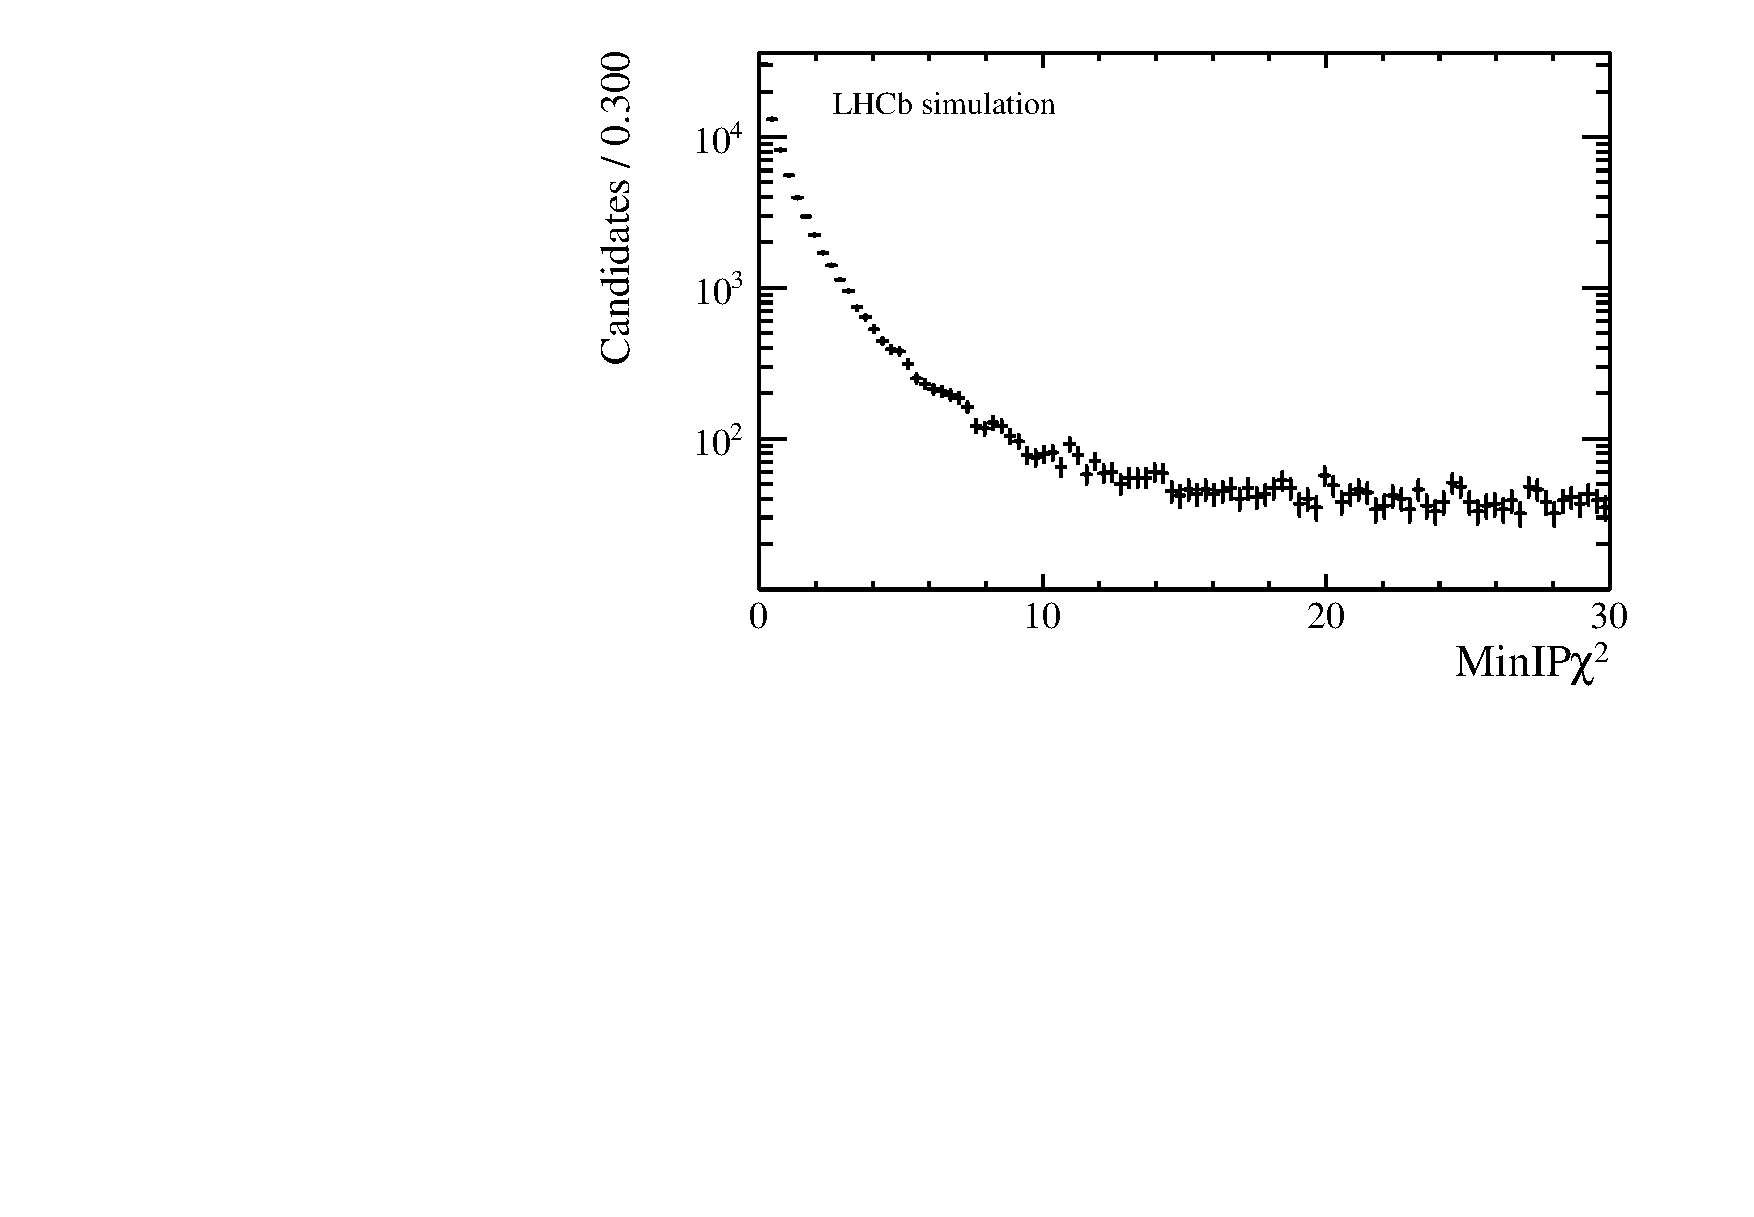
\includegraphics[width=0.45\textwidth]{06selection/figs/MinIPCHI2.pdf}
    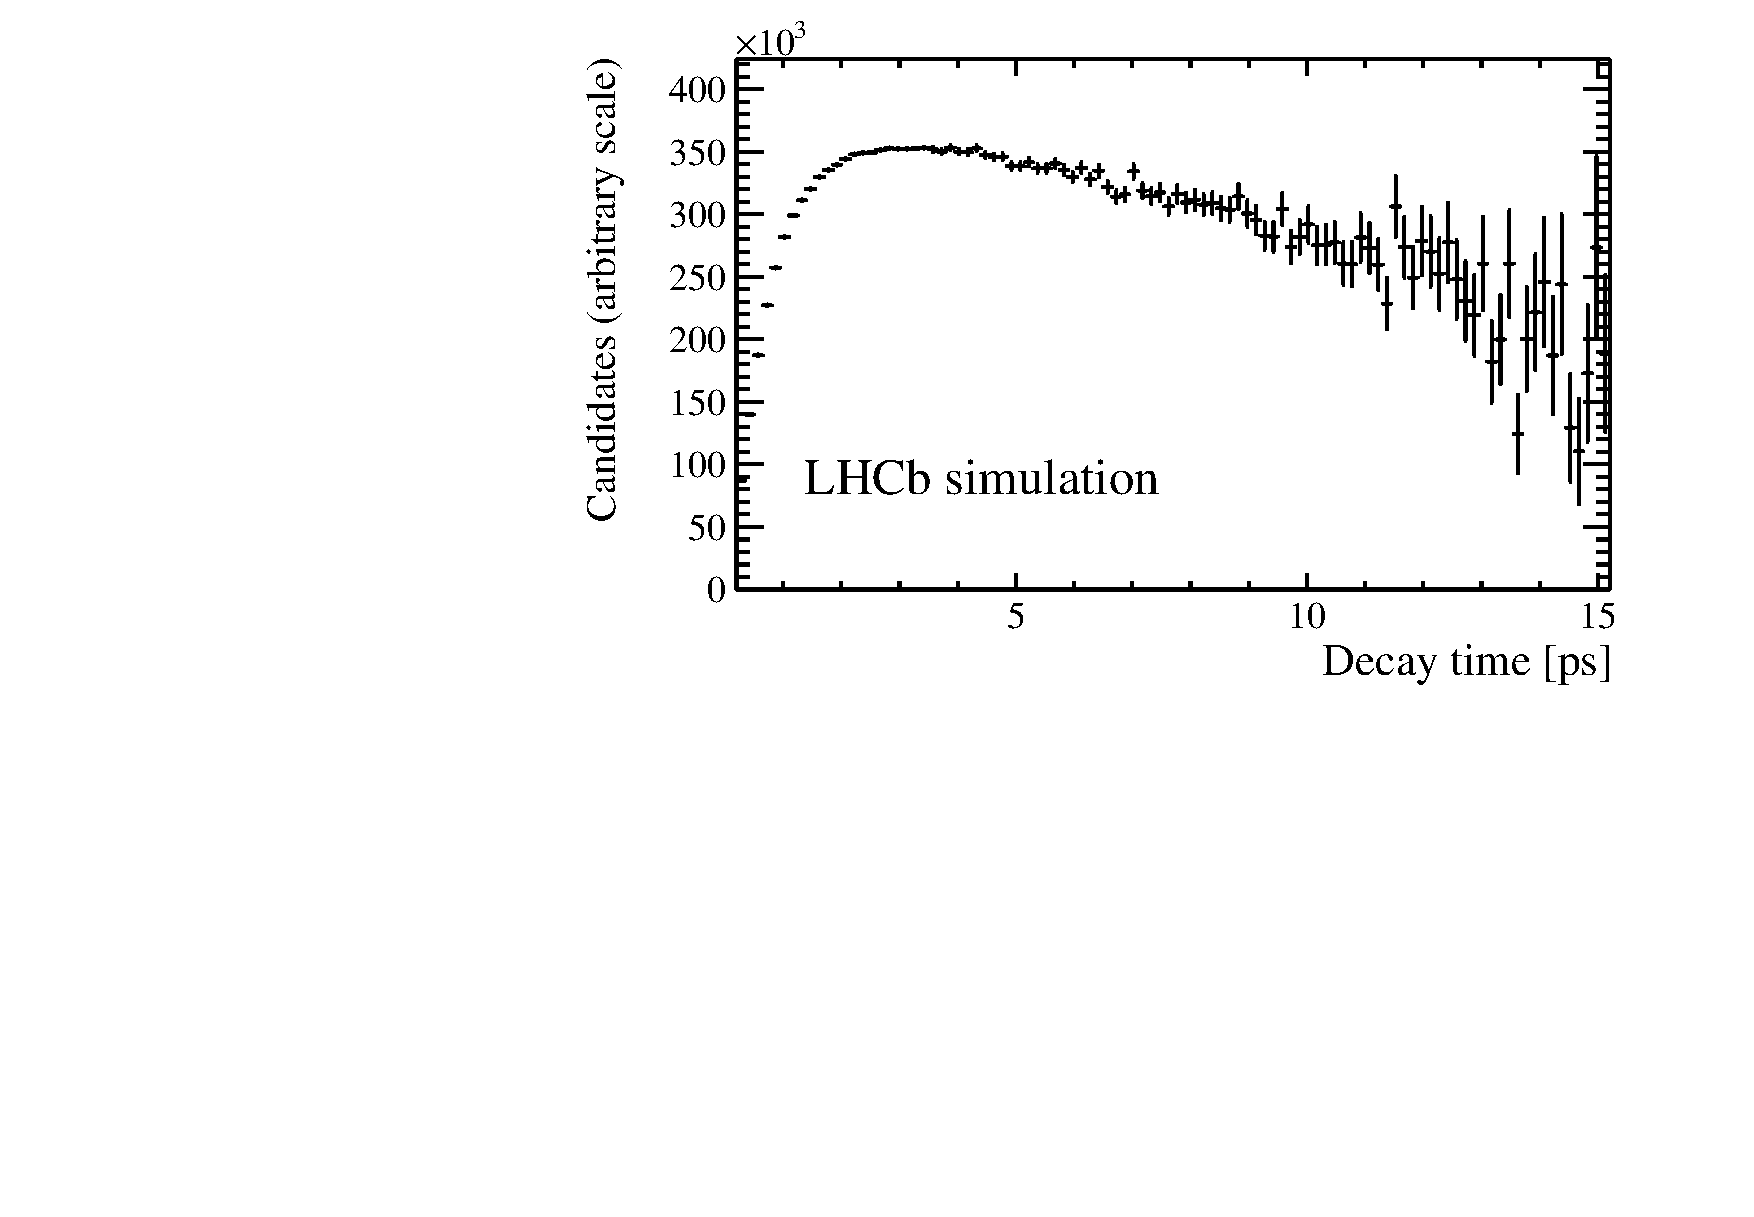
\includegraphics[width=0.45\textwidth]{06selection/figs/WrongPVs-WeightingGoodData.pdf}
    \caption{Left: Distribution of the $\text{MinIP}\chi^2$ variable with the chosen cut point in a narrow range.
    For larger values of $\text{MinIP}\chi^2$ the distribution remains flat.
    Candidates with $\text{MinIP}\chi^2<=16.5$ are rejected.
    Right: Decay time distribution of simulated \BdToDpi candidates, wheighted with an exponential using the true lifetime of the \Bz candidates after applying the cut on $\text{MinIP}\chi^2$.
    The expected acceptance distribution at \lhcb is visible.}
    \label{fig:WrongPVData}
\end{figure}

In contrast the \ac{PV} could also be chosen using some \enquote{best} \ac{PV} criterion, \eg picking the \ac{PV} with the smallest $\text{IP}\chi^2$ w.r.t the \Bz candidate.
Such criterion also removes most of the wrongly associated \ac{PV}s, but potentially biases the decay time distribution, whereas the strategy described above treats all \ac{PV}s equally and thus the decay time distribution remains unbiased.

\subsection{Development of a MVA classifier}
\label{sec:MVADev}

Combinatoric background is suppressed using a \ac{MVA}, more precisely a \ac{BDT} is used.
A \ac{BDT} is a machine learning algorithm for classification.
As all machine learning algorithms it needs to learn, which classes of events should be separated.
Therefore it needs training samples, consisting only of events of the respective classes.
In this case \BdToDpi candidates should be separated from combinatorial background candidates and therefore it needs to be provided with proxies for these classes of candidates.
As proxy for the \BdToDpi candidates, simulation is used based on the conditions of the \num{2012} data taking.
The upper-mass sideband of the \num{2012} data with $m_{\left[\Km\pip\pip\right]\pim}>\SI[per-mode=symbol]{5500}{\MeVcc}$ mimics the background.
Further both proxy samples are divided into a training and a test sample of same size.
When training the \ac{BDT}, the training part is used to actually classify the candidates, while the \ac{BDT} can be applied on the independent test sample to check whether the performance is the same on both samples.
If the performance is different, the \ac{BDT} shows so-called overtraining, \ie the classifier is optimised on statistical fluctuations of the training samples and cannot be applied to other independent samples without a loss in performance.
Another powerful test to check for overtraining is to compare the output distribution of the \ac{BDT} between the training and test sample - again, a difference would indicate that the \ac{BDT} is overtrained.
Since the \ac{BDT} should also in this case learn to separate signal candidates from combinatoric background after applying the vetoes and removing backgrounds like $\Lb\!\to\Lcbar\pip$, all previous selection steps are applied to the signal- and background-proxy samples.

In total, the \ac{BDT} uses \num{16} input variables which are listed in \cref{tab:BDTInput}.
To reduce the number of input variables, from pairs of variables which have a correlation of \SI{97}{\percent} or larger the variable with the smaller separation power is removed.
The final variables cover mostly various $\text{IP}\chi^2$ variables, flight distances, momenta and flight directions.
Furthermore, the $\chi^2$ of the DTF with a constraint on the \ac{PV} is added, as it shows a good separation power between \BdToDpi signal candidates and combinatoric background candidates.
\begin{table}[tbp]
	\centering
	\caption{List of input variables used in the training of the BDT}
	\begin{tabular}{cc}
		\toprule
		\multirow{2}{*}{\Bz candidate}	& $\cos$ of $\sphericalangle\left[\left|\text{PV},\text{SV}\right|,\vec{p}\!(\Bz)\right]$ \\
										& \ac{SV} $\chi^2$\\
		\midrule
		\multirow{7}{*}{\Dm candidate}	& $\text{IP}\chi^2$ w.r.t. the \ac{SV}\\
										& $\text{IP}\chi^2$ w.r.t. the associated PV\\
										& radial flight distance\\
										& flight distance $\chi^2$ w.r.t. the \ac{SV}\\
										& \Dm-vertex $\nicefrac{\chi^2}{\text{ndof}}$\\
										& transverse momentum \pt \\
										& $\cos$ of $\sphericalangle\left[\left|\text{SV},\Dm\text{-Vtx}\right|,\vec{p}\!(\D)\right]$ \\
		\midrule
		\multirow{3}{*}{bachelor \pion}	& $\text{IP}\chi^2$ w.r.t. the associated PV\\
										& transverse momentum \pt\\
										& track $\nicefrac{\chi^2}{\text{ndof}}$\\
		\midrule
		\Dm daughters					& $\text{IP}\chi^2$ of the associated \ac{PV}\\
		\midrule
		DTF 							& $\chi^2$ of the DTF with \ac{PV} constraint \\
		\bottomrule
	\end{tabular}
	\label{tab:BDTInput}
\end{table}
For the \ac{BDT} the implementation from TMVA~\cite{Hocker:2007ht} is used.
The \ac{BDT} consists of \num{1700} decision trees with a maximum depth of four.
The variables are scanned at \num{20} points to find the optimal cut value and each node has to contain at least \SI{2.5}{\percent} of the training candidates.
As boosting algorithm AdaBoost~\cite{AdaBoost} is chosen with a boost factor $\beta=0.5$.
The approach to find this configurations is iteratively, \ie the complexity of the \ac{BDT} is increased as long as no overtraining is visible.
The final overtraining check is shown in \cref{fig:BDTOVertraining}.
\begin{figure}[tbp]
    \centering
    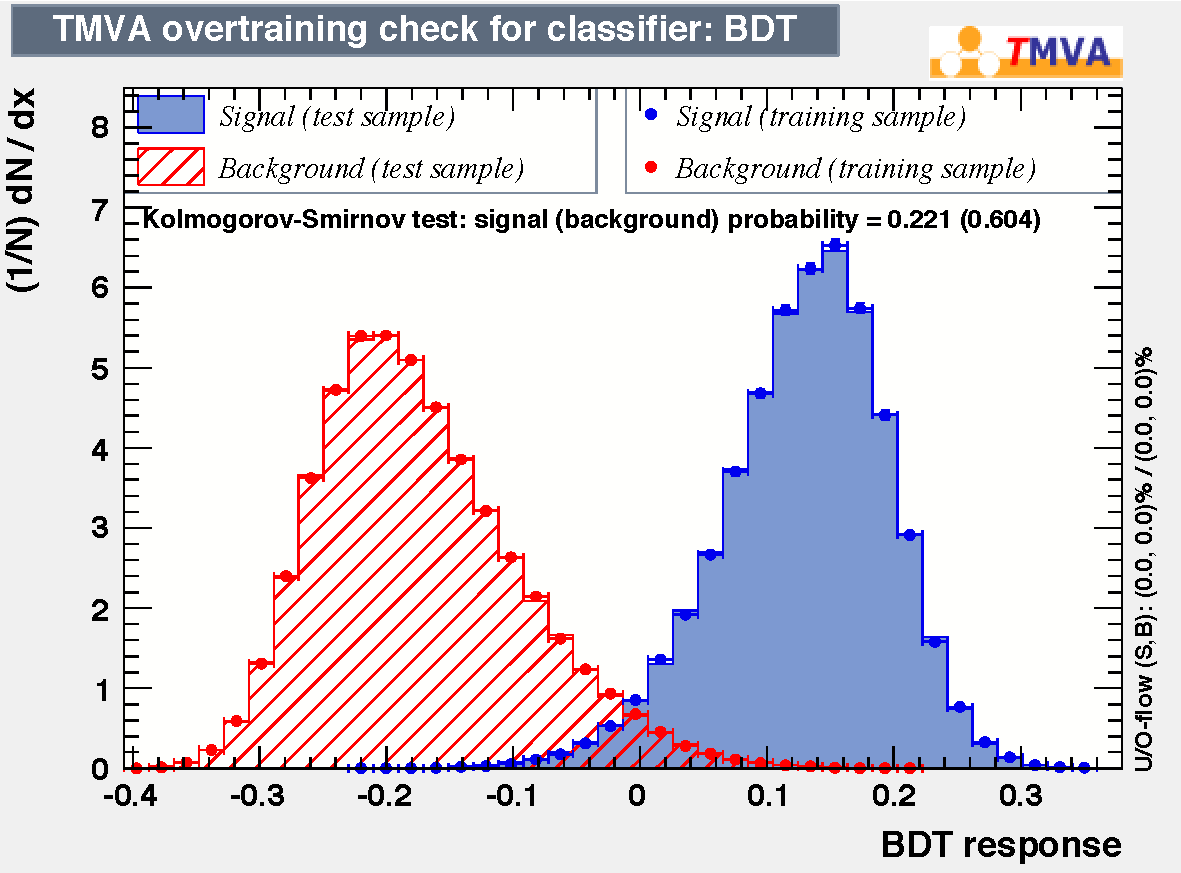
\includegraphics[width=0.7\textwidth]{06selection/figs/overtrain_BDT.pdf}
    \caption{Comparison of \ac{BDT} responses on the training and test sample.}
    \label{fig:BDTOVertraining}
\end{figure}
The agreement between the \ac{BDT} output distributions on the training and test samples is also checked with a Kolmogorov-Smirnov test~\cite{Bohm:389738} which gives \num{0.221} and \num{0.604} for the signal and background samples and thus indicates a good agreement.

\subsection{BDT selection optimisation}
\label{sec:BDTOpt}

To optimise the cut on the \ac{BDT} response the uncertainties on the \CP parameters \Sf and \Sfbar are used.
For the optimisation all preselection cuts, the vetoes for background from semileptonic decays and $\Lb\!\to\Lcbar\pip$ decays and the veto for wrongly associated \ac{PV}s are applied to the full dataset of both Run I.
To determine the uncertainty of \Sf and \Sfbar depending on the \ac{BDT} response the following strategy is adopted:
The \ac{BDT} output is scanned with a step size of \num{0.01} within a narrow range from \numrange{-0.15}{0.1} and with a step size of \num{0.05} in the outer regions.
For each cut on the \ac{BDT} response a fit to the invariant \Bz mass in the range \SIrange[per-mode=symbol]{5200}{5500}{\MeVcc} using the \emph{pion}-sample is performed.
This fit is used to determine \emph{sWeights}~\cite{Pivk:2004ty} and to obtain the mass shape which corresponds to the respective cut on the \ac{BDT} output.
Applying the \emph{sWeights} to other observables such as the decay time makes these distributions appear like signal-only~\cite{2009arXiv0905.0724X}.
Therefore, using \emph{sWeights} the tagging efficiencies, the shapes of the mistag distributions of the OS and SS tagging algorithms (more details on the flavour tagging can be found in \cref{ch:flavourtagging}) and the shape of the decay-time acceptance are obtained for the \enquote{signal} distributions.
The shape of the last is obtained in the same way as described in \cref{sec:acceptance}.
For each cut point then a single pseudoexperiment is performed: The invariant mass distribution is generated using the obtained signal and background yields and shapes from the mass fit, for the mistag and decay time distribution signal and background are both generated using the signal shapes.
The generated values for the \CP parameters are taken from simulation.
This pseudoexperiment sample is then fitted back: After determining \emph{sWeights} from a fit to the invariant \Bz mass distribution, a \CP fit to the decay time distribution is performed, where the flavour tagging calibration is assumed to be perfect.
In \cref{fig:BDTopt} the uncertainties on \Sf and \Sfbar are shown as a function of the \ac{BDT} response.
The final cut point is chosen at the right end of the plateau at \num{0.0}, to have as few background as possible while achieving the best possible sensitivity.
\begin{figure}[tbp]
    \centering
    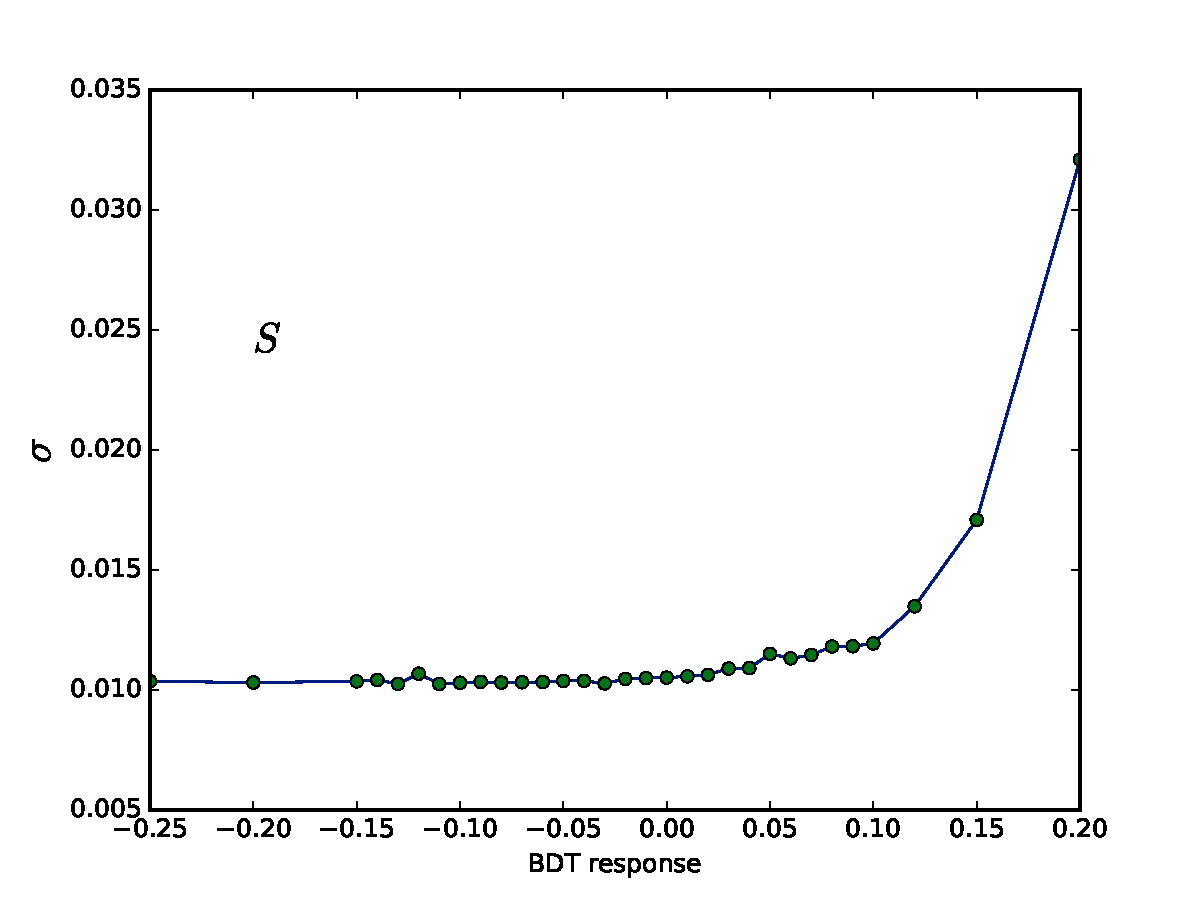
\includegraphics[width=0.49\textwidth]{06selection/figs/sensitiv_Sf.pdf}
    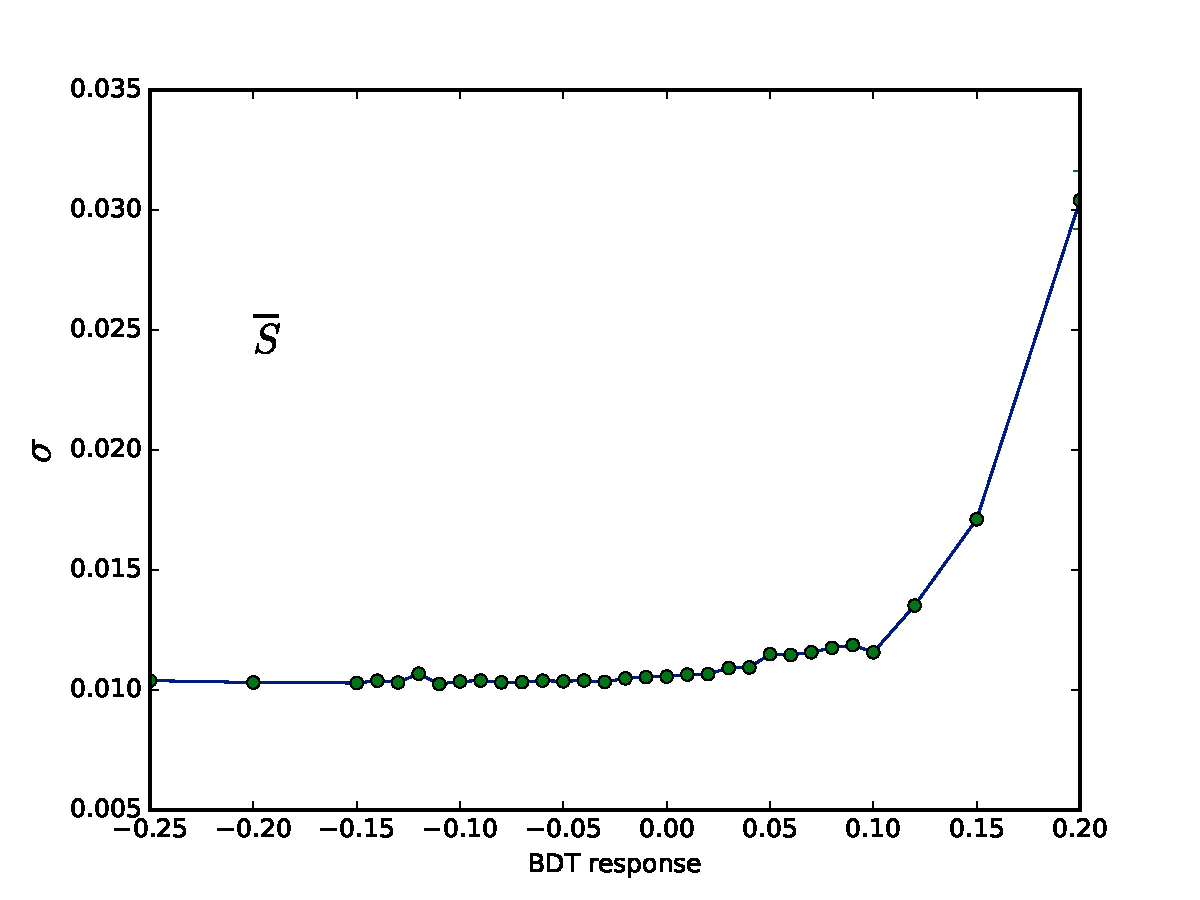
\includegraphics[width=0.49\textwidth]{06selection/figs/sensitiv_Sfbar.pdf}
    \caption{Uncertainty on \Sf (left) and \Sfbar (right) as a function of the \ac{BDT} response.}
    \label{fig:BDTopt}
\end{figure}

\subsection{Multiple candidates}
\label{sec:MultCands}

In the stripping and trigger all used variables rely on the association of the \Bz candidate with the \ac{PV} to which the candidate has the smallest $\text{IP}\chi^2$, also denoted as best \ac{PV}.
To be consistent with this strategy for each event also the best \ac{PV} is chosen.
Events where the formerly best \ac{PV} is no longer present after the selection are removed.
Besides, events can contain more than one \Bz candidate.
After the stripping this is the case for \SI{9}{\percent} of the events and \SIrange{18}{20}{\percent} of the \Bz candidates share the same event.
This is reduced after applying the described selection steps, so that after selection only \SI{0.4}{\percent} of the events contain multiple candidates and \SI{0.8}{\percent} of the \Bz candidates share one event.
Following the proposal in \cite{Koppenburg:2017zsh} the remaining candidates are assumed to be equally likely signal candidates and one candidate per event is chosen at random.

\subsection{Selection performance}
\label{sec:selectionPerformance}

The final selection performance is determined on the upper mass sideband with \mbox{$m_{\left[\Km\pip\pip\right]\pim}>\SI[per-mode=symbol]{5500}{\MeVcc}$} of the data and simulation based on the conditions of the \num{2012} data taking.
The corresponding signal efficiencies $\varepsilon_{\text{sig}}$ and background rejections $1-\varepsilon_{\text{bkg}}$ are given in \cref{tab:selPerform}.
\begin{table}[tbp]
	\centering
	\caption{Performances of all selection steps, where background refers to combinatorial background candidates.
	All efficiencies are calculated using the number of candidates after the previous selection step as \SI{100}{\percent}.
	The overall performance is given in the last row.}
	\begin{tabular}{ccc}
		\toprule
		Selection step						& $\varepsilon_{\text{sig}}$  & $1-\varepsilon_{\text{bkg}}$ \\
		\midrule
		preselection						& \SI{93.61\pm0.06}{\percent} & \SI{85.20\pm0.02}{\percent} \\
		\midrule
		$\Lz^\pm_\cquark$-veto				& \SI{93.48\pm0.06}{\percent} & \SI{9.85\pm0.03}{\percent} \\
		semileptonic veto					& \SI{98.96\pm0.03}{\percent} & \SI{7.66\pm0.03}{\percent} \\
		mass vetoes combined				& \SI{92.51\pm0.07}{\percent} & \SI{16.77\pm0.04}{\percent} \\
		\midrule
		wrongly associated \ac{PV}s veto	& \SI{97.75\pm0.04}{\percent} & \SI{15.81\pm0.04}{\percent} \\
		BDT selection						& \SI{83.63\pm0.10}{\percent} & \SI{97.18\pm0.01}{\percent} \\
		\midrule
		overall								& \SI{70.7\pm0.1}{\percent}   & \SI{99.911\pm0.002}{\percent} \\
		\bottomrule
	\end{tabular}
	\label{tab:selPerform}
\end{table}
The low background suppression of the vetoes is expected, as the vetoes aim to suppress specific backgrounds, but not the combinatorial background which is used to determine the given efficiencies.

Finally, the contamination with non resonant $\Bz\to\Kp\pim\pim\pip$ decays is determined, as such background would show the same structure as \BdToDpi candidates in the invariant $m_{\Kp\pim\pim\pip}$-distribution, but the \emph{weak} phase would be different.
In order to do this, two strategies are implemented, both using the datasample after applying all selection steps, except for the cut on the invariant \Dm-mass described in \cref{tab:preselection}:
For the first strategy the invariant \Dm-mass is plotted for candidates in a tight \Bz signal window from \SIrange[per-mode=symbol]{5240}{5320}{\MeVcc} as shown in \cref{fig:nonRes_Try1}.
\begin{figure}[tbp]
    \centering
    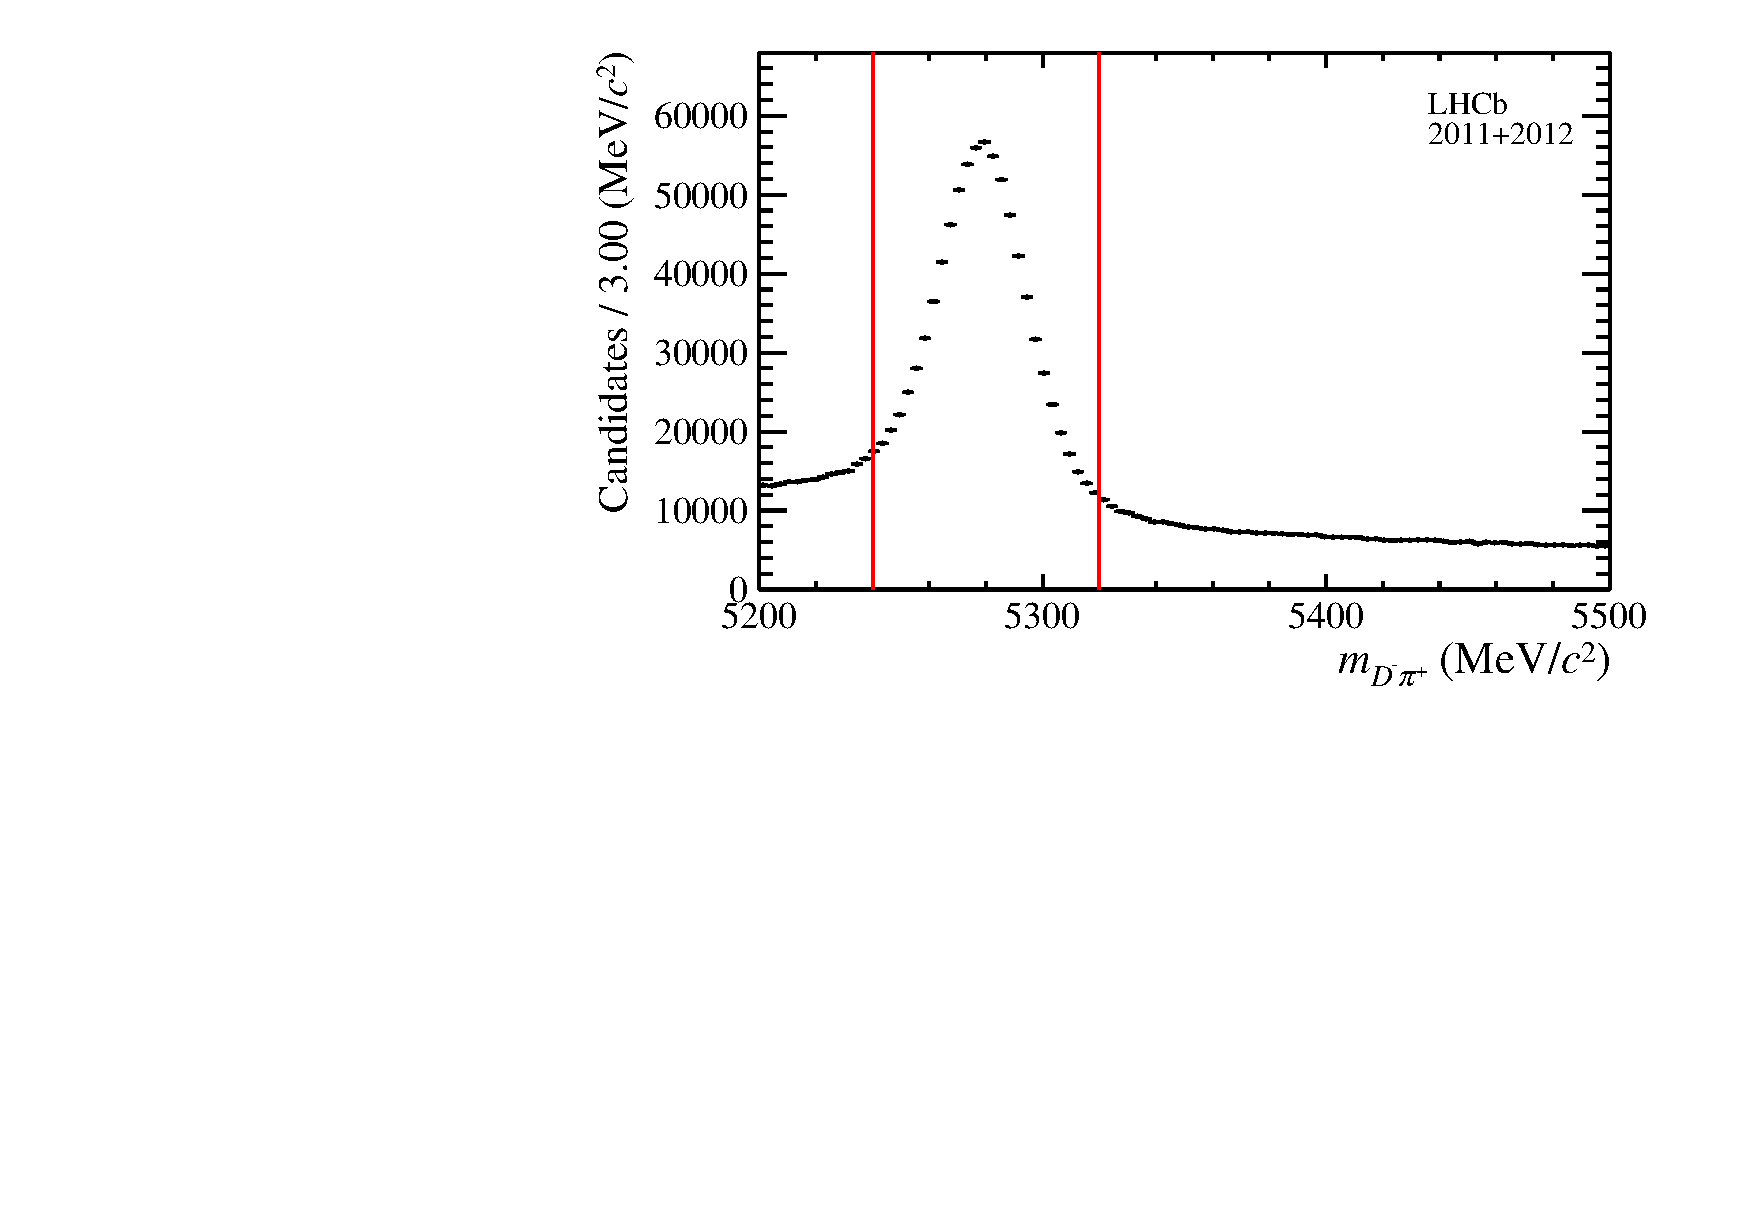
\includegraphics[width=0.49\textwidth]{06selection/figs/BmassCut.pdf}
    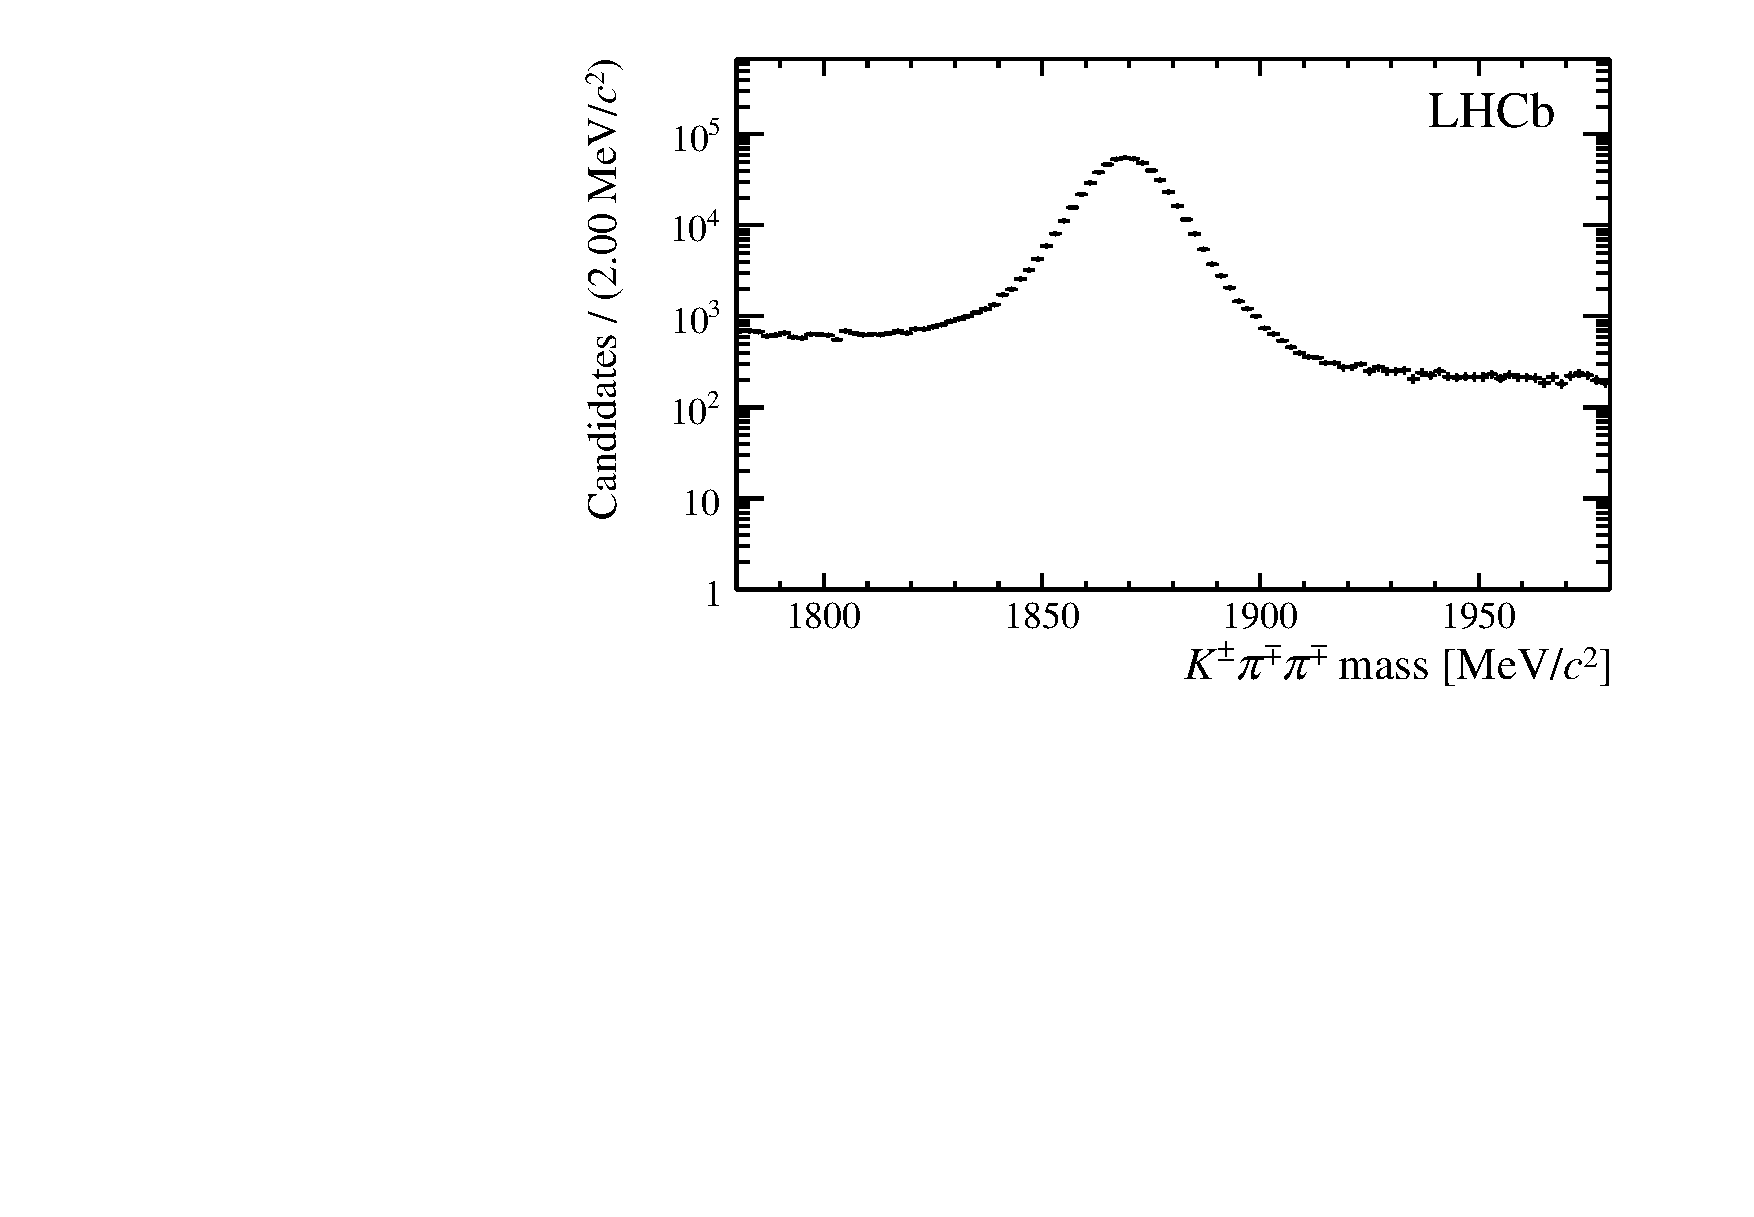
\includegraphics[width=0.49\textwidth]{06selection/figs/Resulting_Dmass.pdf}
    \caption{Left: Invariant \Bz-mass distribution with the selected signal region between the red vertical lines.
    Right: Resulting invariant \Dm-mass distribution.}
    \label{fig:nonRes_Try1}
\end{figure}
From the invariant \Dm-mass distribution the non-resonant contamination can be estimated to be roughly \SI{1}{\percent}.
In the second strategy a cut on the invariant \Dm-mass distribution removing the \Dm-peak is applied.
Then the invariant \Bz-mass without constraint on the \Dm-mass is inspected and a fit using an exponential to model the background and a gaussian with fixed shape to model the signal is performed to estimate the number of non-resonant $\Bz\!\to\Kp\pim\pim\pip$ candidates (see \cref{fig:nonRes_Try2}).
\begin{figure}[tbp]
    \centering
    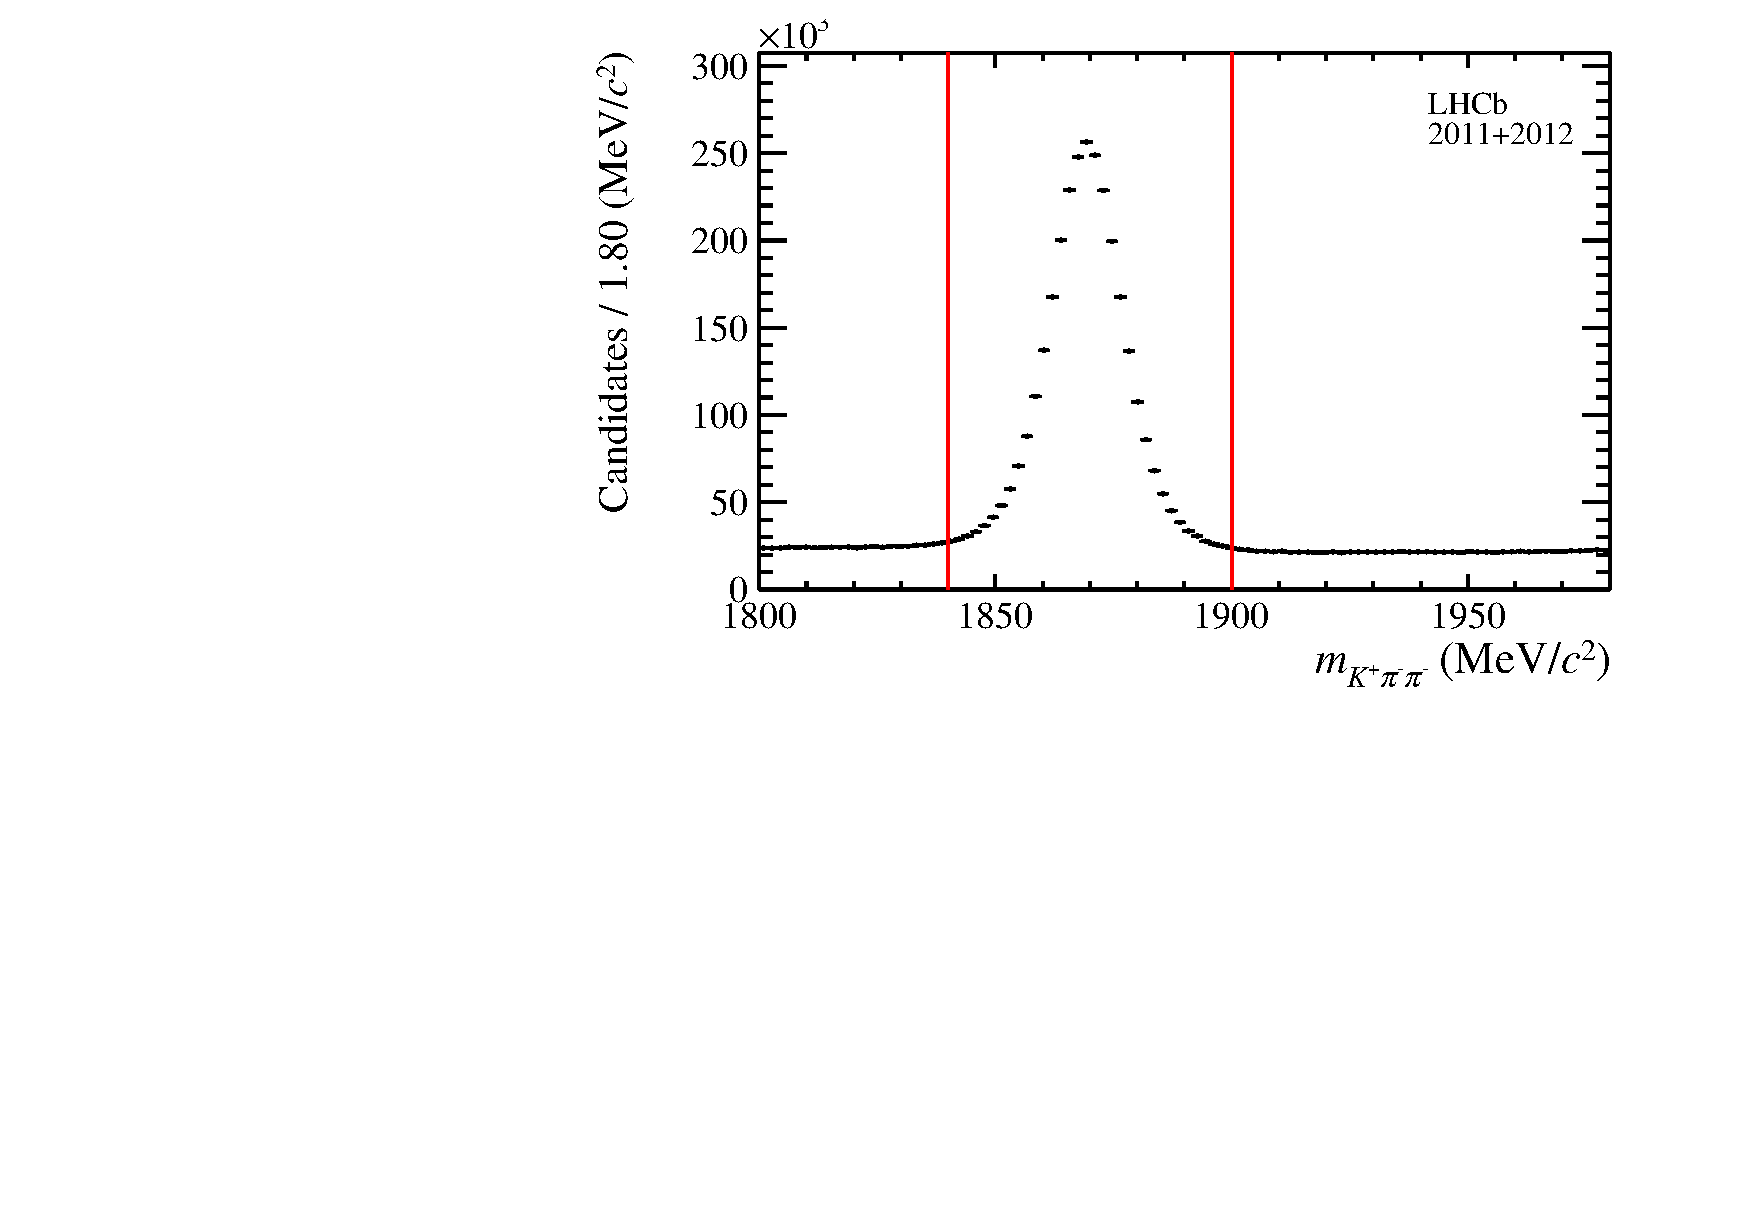
\includegraphics[width=0.49\textwidth]{06selection/figs/DmassCut.pdf}
    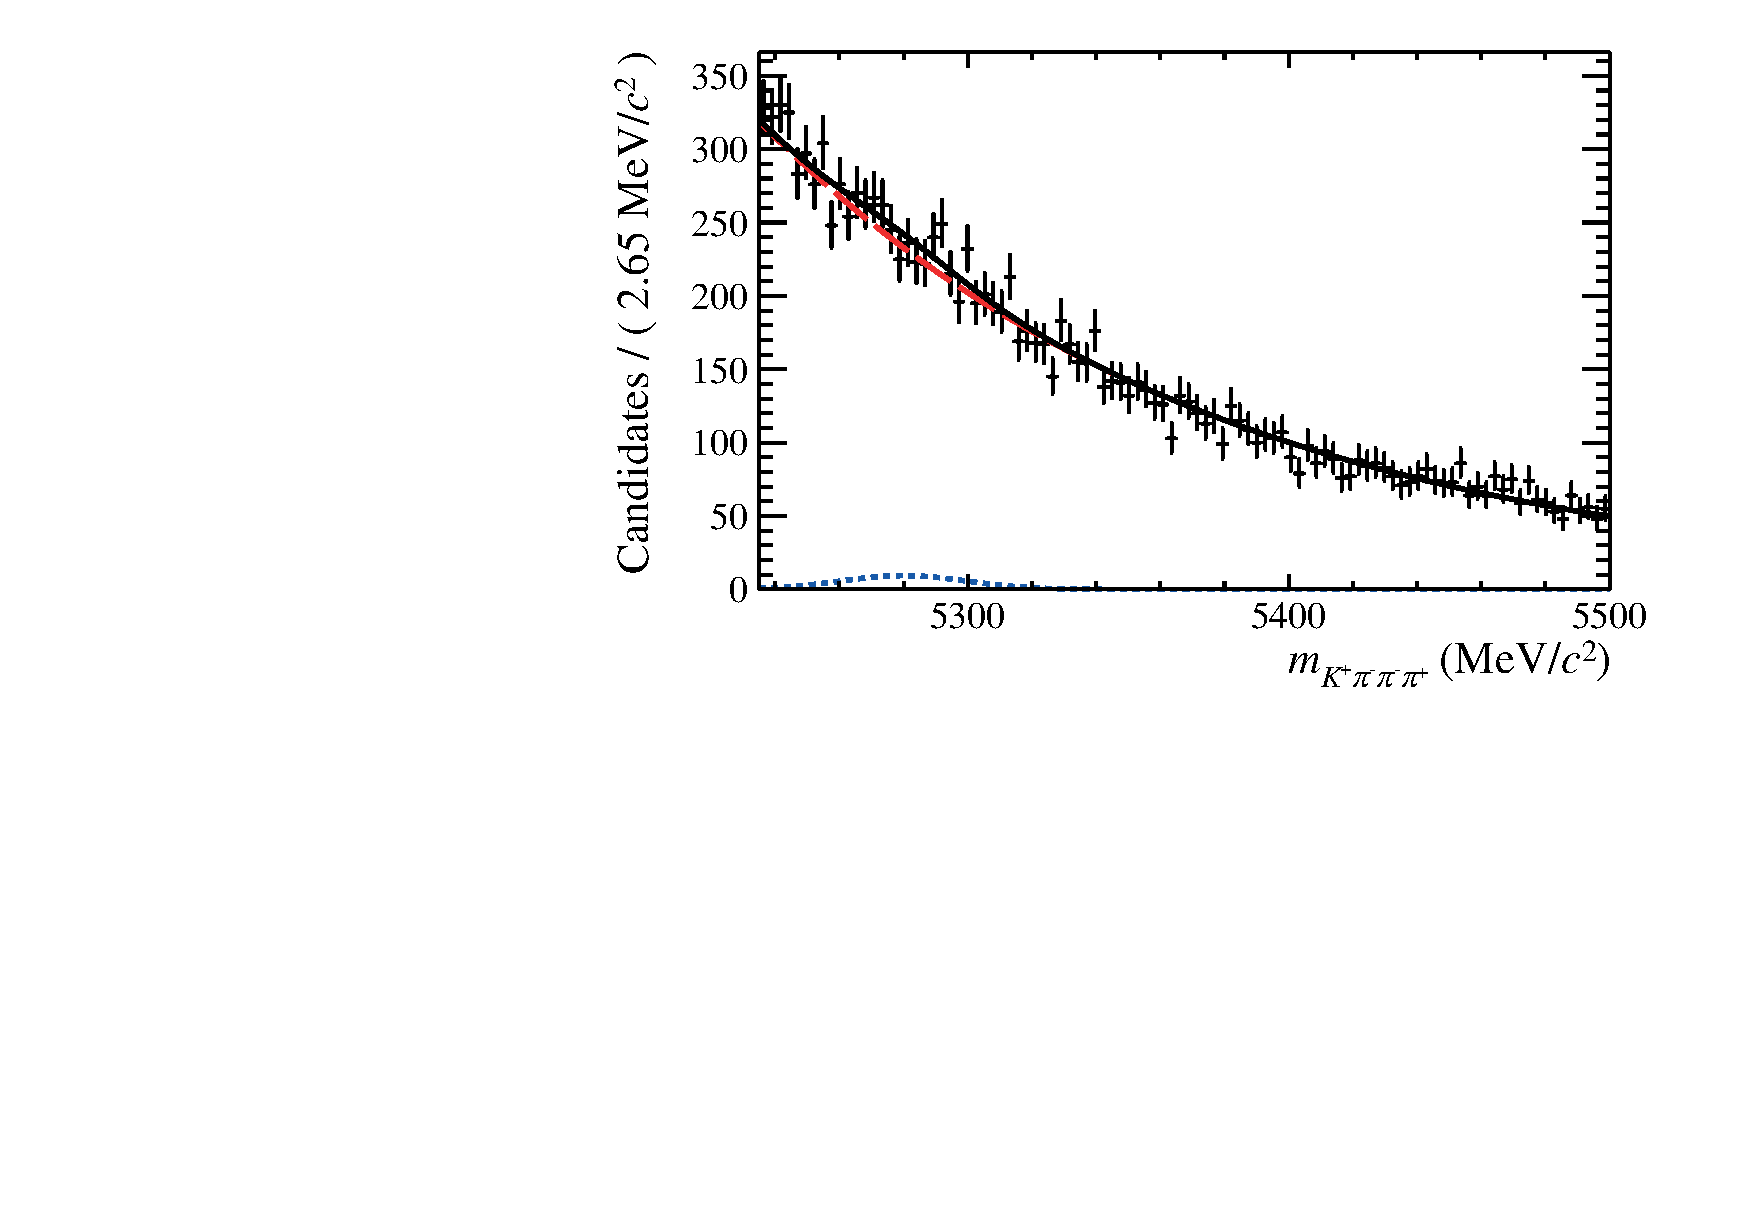
\includegraphics[width=0.49\textwidth]{06selection/figs/Resulting_Bmass.pdf}
    \caption{Left: Invariant \Dm-mass distribution with the excluded signal region between the red vertical lines.
    Right: Resulting invariant \Bz-mass distribution with the fit overlaid. The red dashed line describes the combinatorial background, the blue dotted line the signal component.}
    \label{fig:nonRes_Try2}
\end{figure}
This fit yields \num{645\pm242} signal candidates.
As both strategies do not show a significant amount of a non-resonant contamination of the sample, this is assumed to be negligible.

  % % !TEX root = main.tex
\chapter{Mass fit}
\label{ch:massfit}

\linespread{1.08}\selectfont
After selection the datasample is split into the two samples described in \cref{sec:Samples}, referred to as \emph{pion}- and \emph{kaon}-sample.
The invariant \Bz mass distributions of candidates with a tag of one of the flavour tagging algorithms are fitted simultaneously in these samples in order to calculate \emph{sWeights}~\cite{Pivk:2004ty}, which are used in the following analysis steps to separate signal from background candidates statistically.
Before reporting in greater detail about these fits it is important to note that the work described in this chapter was done by a collaborator.
However, since this is an essential part of the analysis required to follow the subsequent steps, it is not omitted completely, but the extent to which \eg experimental techniques are described is less comprehensive compared to the other parts.

When parametrising the invariant \Bz mass all components contributing need to be described. Backgrounds from semileptonic decays, $\Lb\!\to\Lcbar\pip$ decays and $\Bs\!\to\Dsm\pip$ decays is either removed in the selection or found to be at a negligible level.
However, beside the signal component and the combinatorial background both, the \emph{pion}- and \emph{kaon}-sample show additional backgrounds which arise due to missing neutral particles in the reconstruction or pion-kaon-misidentifications.
In the \emph{pion}-sample contributions from $\Bz\!\to\Dm\rhop\!\left(\to\pip\piz\right)$ and $\Bz\!\to\Dstarm\!\left(\to\Dm\piz/\g\right)\pip$ decays arise, the \emph{kaon}-sample shows a component from $\Bz\!\to\Dm\Kstarp\!\left(\to\Kp\piz\right)$ and also $\Bz\!\to\Dm\rhop\!\left(\to\pip\piz\right)$  needs to be described.
Furthermore, both samples show a cross-feed component from each other.
Using the efficiencies of the \dllkpi requirement on simulations $\varepsilon_{\text{PID}}\!\left(\Bz\!\to\D X\right)_Y$ (with $X, Y=\pion, \kaon$) the number of cross-feed $\Bz\!\to\D\kaon$ candidates in the \emph{pion}-sample can be expressed from the yield in the \emph{kaon}-sample and vice versa as
\begin{equation}
\begin{aligned}
N_{\Bz\!\to\D\pion}^{\kaon}&=\frac{1-\varepsilon_{\text{PID}}\!\left(\Bz\!\to\D \pion\right)_{\pion}}{\varepsilon_{\text{PID}}\!\left(\Bz\!\to\D \pion\right)_{\pion}}\times N_{\Bz\!\to\D\pion}^{\pion} \,\,,\\
N_{\Bz\!\to\D\kaon}^{\pion}&=\frac{1-\varepsilon_{\text{PID}}\!\left(\Bz\!\to\D \kaon\right)_{\kaon}}{\varepsilon_{\text{PID}}\!\left(\Bz\!\to\D \kaon\right)_{\kaon}}\times N_{\Bz\!\to\D\kaon}^{\kaon}\,\,.\label{eq:ConstrainCrossFeed}
\end{aligned}
\end{equation}
Hereby the superscripts denote the sample and the subscript the component within the respective sample.

Before describing the mass fit to data {\cref{sec:MassFitData}}, first the probability density functions (PDFs) used for the different components are introduced in the following (\cref{sec:PDFs}).

\section{Probability densitiy functions}
\label{sec:PDFs}

The various peaking components in the invariant mass distributions are described by a phenomenological approach, where the description is first
estimated on simulated decays.
In contrast, the combinatorial background is determined directly in the fit to data.
For the \emph{pion}-sample the following PDFs are used to parameterise the peaking components:
\begin{itemize}
	\item $\Bz\!\to\Dpm\pimp$: The signal component is described by a double-sided Hypatia and a Johnson SU function.
	The Hypatia~\cite{Santos:2013ky} is defined as
	\begin{equation}
	\begin{aligned}
	&\mathcal{I}(m;\mu,\sigma,\lambda,\zeta,\beta,a_1,n_1,a_2,n_2) \propto\\
	&\hspace{2.8cm}\begin{cases}
	G(m,\mu,\sigma,\lambda,\zeta,\beta,a,n), &\,   - a_1 < \frac{m - \mu}{\sigma} < a_2 \\
	\frac{G(\mu - a_1 \sigma,\mu,\sigma,\lambda,\zeta,\beta)}{\left(1 - m/(n \frac{G(\mu - a_1\sigma,\mu,\sigma,\lambda,\zeta,\beta)}{G^\prime(\mu - a_1 \sigma,\mu,\sigma,\lambda,\zeta,\beta)} -a_1 \sigma)\right)^{n_1}},	&\,  - a_1 > \frac{m - \mu}{\sigma} \\
	\frac{G(\mu - a_2 \sigma,\mu,\sigma,\lambda,\zeta,\beta)}{\left(1 - m/(n \frac{G(\mu - a_2\sigma,\mu,\sigma,\lambda,\zeta,\beta)}{G^\prime(\mu - a_2 \sigma,\mu,\sigma,\lambda,\zeta,\beta)} -a_2 \sigma)\right)^{n_2}},	&\quad a_2 < \frac{m - \mu}{\sigma} \\
	\end{cases}
	\label{eq:ipatia}
	\end{aligned}
	\end{equation}
	with
	\begin{equation}
	\begin{aligned}
	&G(m,\mu,\sigma,\lambda,\zeta,\beta,a,n)\propto\\
	&\hspace{0.6cm}\left(\left(m-\mu\right)^2+A_\lambda^2(\zeta)\sigma^2\right)^{\frac{1}{2}\lambda-\frac{1}{4}}e^{\beta\left(m-\mu\right)}K_{\lambda-\frac{1}{2}}\left(\zeta\sqrt{1+\left(\frac{m-\mu}{A_\lambda(\zeta)\sigma}\right)^2}\right)\,.
	\end{aligned}
	\end{equation}
	Defining the quantities
	\begin{align*}
	&w=e^{r^2}\,,&\\
	&\omega=-\nu\tau\,,&\\
	&c=\frac{1}{\sqrt{\frac{1}{2}\left(w-1\right)\left(w\cosh\!\left(2\omega\right)+1\right)}}\,,&\\
	&z=\frac{m-\left(\mu+c+\sigma\sqrt{w}\sinh\omega\right)}{c\sigma}\,,&\\
	&r=-\nu+\frac{\sinh^{-1}z}{\tau}\,,&
	\end{align*}
	the Johnson SU function~\cite{JohnsonSU} can be expressed as
	\begin{equation}
	\mathcal{J}\!\left(m;\mu,\sigma,\nu,\tau\right)\propto\frac{1}{2\pi c(\nu,\tau)\sigma}e^{-\frac{1}{2}r(m;\mu,\sigma,\nu,\tau)^2}\frac{1}{\tau\sqrt{z(m;\mu,\sigma,\nu,\tau)^2+1}}\,.\label{eq:johnsonsu}
	\end{equation}
	\item $\Bz\!\to\Dm\Kp$: The cross-feed component is parametrised by a double-sided Hypatia function as described in \cref{eq:ipatia}.
	\item $\Bz\!\to\Dm\rhop$: The first partially reconstructed background is described by a single-sided Crystal Ball function and a Gaussian function.
	The single-sided Crystal Ball function is defined as
	\begin{equation}
	\mathcal{C\!B}\!\left(m;\mu,\sigma,\alpha,n\right)\propto\begin{cases}
	e^{-frac{(m-\mu)^2}{2\sigma^2}}, &\, \frac{m-\mu}{\sigma}>-\alpha\\
	A\left(B-\frac{m-\mu}{\sigma}\right)^{-n}, &\, \frac{m-\mu}{\sigma}\leq-\alpha\\\end{cases}\label{eq:CrystalBall}
	\end{equation}
	with
	\begin{equation}
	A=\left(\frac{n}{\left|\alpha\right|}\right)^{n}e^{-\frac{\left|\alpha\right|^2}{2}}\hspace{0.5cm}\text{ and }\hspace{0.5cm}B=\frac{n}{\left|\alpha\right|}-\left|\alpha\right|\,.
	\end{equation}
	\item $\Bz\!\to\Dstarm\pip$: The second-partially reconstructed component is modelled with the sum of a single-sided Crystal Ball function (\cref{eq:CrystalBall}) and a Gaussian function.
\end{itemize}
For the \emph{kaon}-sample the peaking components are modelled as following:
\begin{itemize}
	\item $\Bz\!\to\Dm\Kp$: The signal component ist described with a single-sided Hypatia function. The single-sided Hypatia can be derived from the double-sided Hypatia function as described in \cref{eq:ipatia} by setting the parameters $n_2=0$ and $a_2\to+\infty$, \ie fixing $a_2$ to a large value.
	\item $\Bz\!\to\Dpm\pimp$: The cross-feed component is parametrised by a double-sided Hypatia function as described in \cref{eq:ipatia}.
	\item $\Bz\!\to\Dm\rhop$: The partially-reconstructed and further misidentified background is parametrised by a sum of two Gaussian functions. The sum is normalised using fractions $f$ and $1-f$ for the two Gaussian functions.
	\item $\Bz\!\to\Dm\Kstarp$: The partially reconstructed background is modelled with a Gaussian function.
\end{itemize}
The combinatorial background is described with a sum of two exponentials in the \emph{pion}-sample, while for the \emph{kaon}-sample a single exponential function is sufficient.

\section{Fit to data}
\label{sec:MassFitData}

To determine \emph{sWeights} the invariant \Bz mass is fitted with a two-stage strategy:
First, a simultaneous binned extended maximum-likelihood fit in the invariant-mass range $[5090, 6000]\,\si[per-mode=symbol]{\MeVcc}$ is performed (Fit A).
This allows to control the contamination with $\Bz\!\to\Dm\Kp$ candidates in the \emph{pion}-samples.
A binned fit is performed due to the very large number of candidates.
In this fit the mean and width parameters of the signal components in the \emph{pion}- and \emph{kaon}-samples are floated, while for the tail parameters the values are taken from simulation, multiplied by a scale factor which is then floated.
All yields in the fit are floating, except for the cross-feed yields which are constrained as shown \cref{eq:ConstrainCrossFeed}, \ie the efficiencies $\varepsilon_{\text{PID}}\!\left(\Bz\!\to\D \pion\right)_{\pion}$ and $\varepsilon_{\text{PID}}\!\left(\Bz\!\to\D \kaon\right)_{\kaon}$ are constrained by means of a Gaussian function.
Furthermore, the mean parameters of the $\Bz\!\to\Dm\Kstarp$ in the \emph{kaon}-sample and of the cross-feed $\Bz\!\to\Dm\Kp$ and \BdToDpi components are floated.
All other parameters are fixed to values determined on simulated events.
In \cref{fig:MassFitPlot} the invariant $\D\pion$  and $\D\kaon$ mass distributions with the fit projections overlaid are shown.
\begin{figure}[tbp]
    \centering
    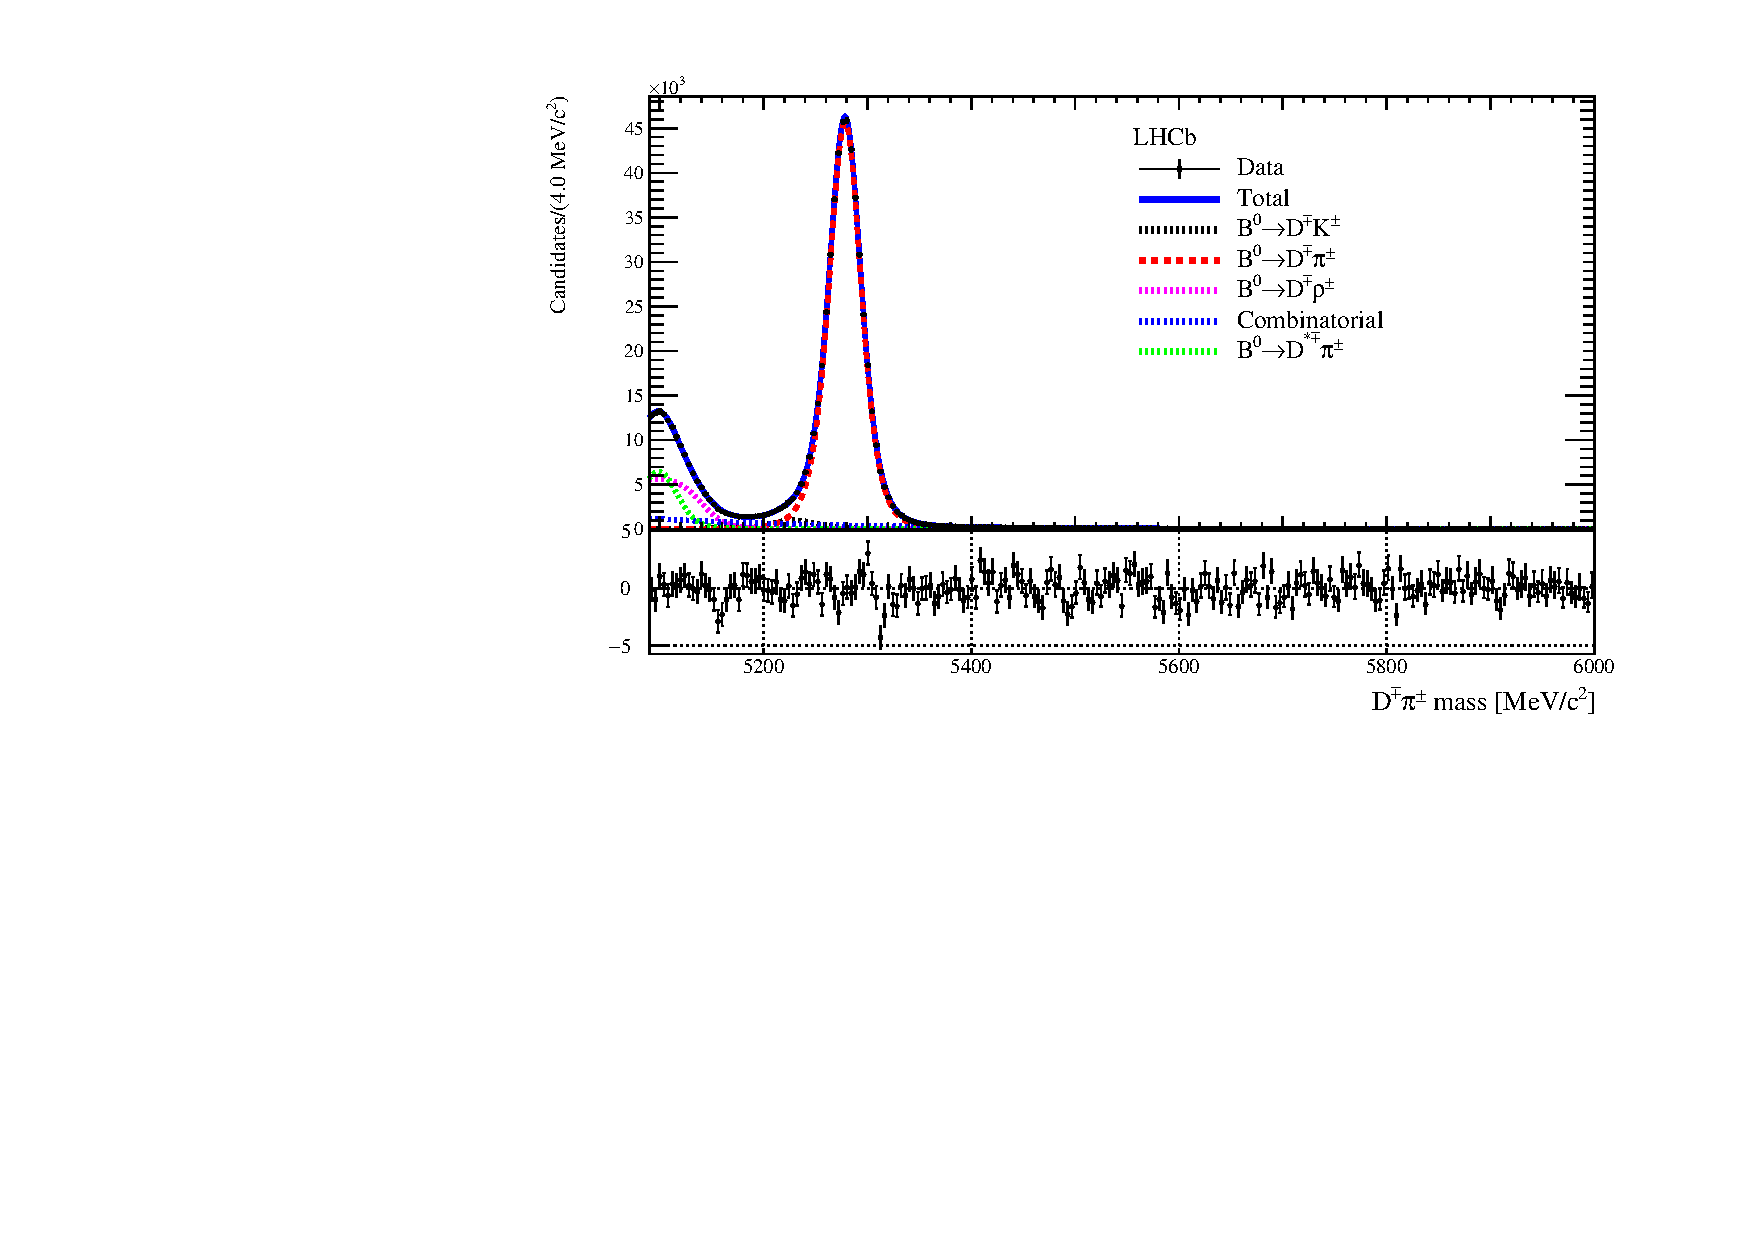
\includegraphics[width=0.75\textwidth]{07MassFit/figs/MDFit_BeautyMass_Bd2DPi_withPulls.pdf}
    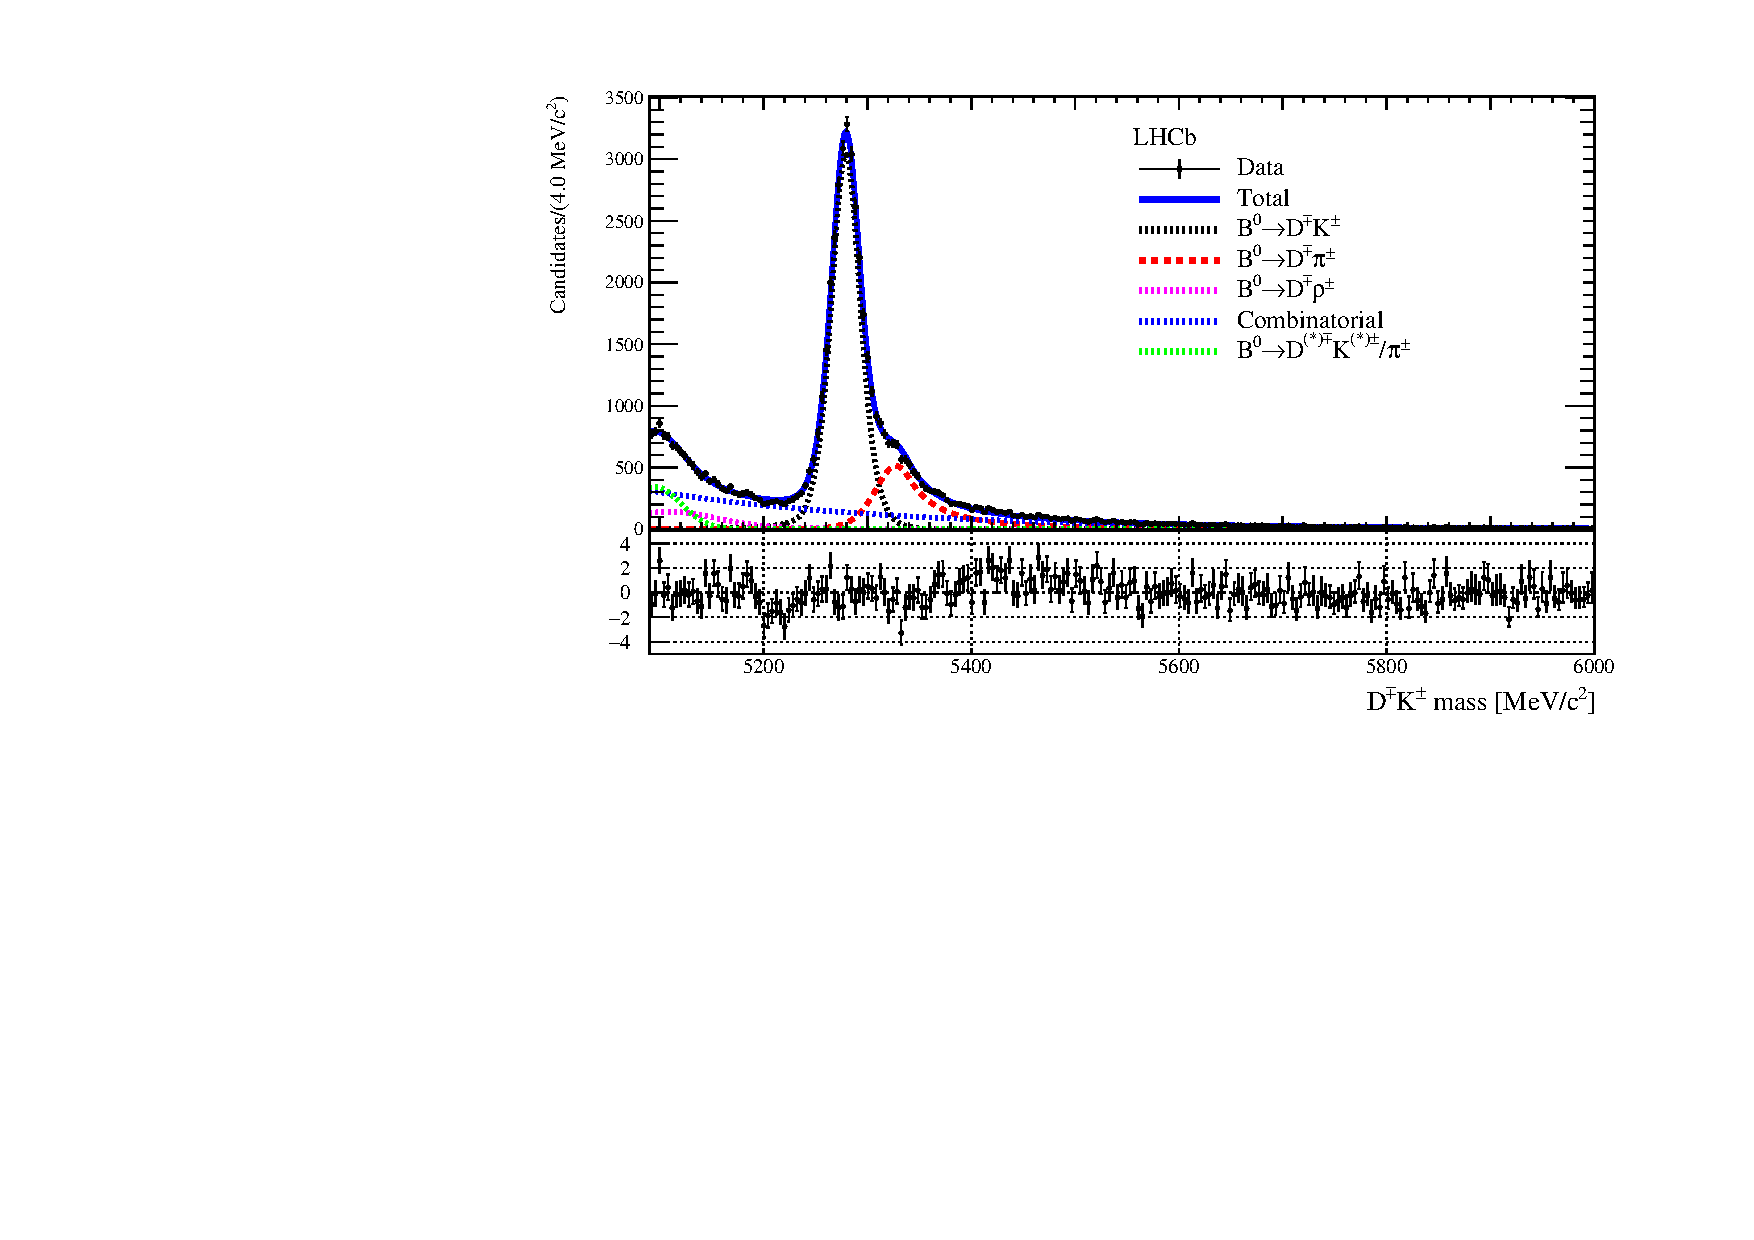
\includegraphics[width=0.75\textwidth]{07MassFit/figs/MDFit_BeautyMass_Bd2DK_withPulls.pdf}
    \caption{Invariant mass distributions of the $\D X$ mass in the \emph{pion}-sample (left) and \emph{kaon}-sample (right).
    The fit projections of Fit A are overlaid.}
    \label{fig:MassFitPlot}
\end{figure}

After Fit A, a unbinned maximum-likelihood fit in the \emph{pion}-sample is performed for which all background components are combined into one single background component and the shapes are fixed to the values found in Fit A.
Futhermore, the fit range is reduced to $[5220, 5600]\,\si[per-mode=symbol]{\MeVcc}$, in order to prevent a dilution of the \emph{sWeights} in later steps of the analysis, as all background components which are neither combinatorial nor close to the signal are removed.
In this second fit (Fit B) only two parameters are floating: The yield $N_{\Bz\!\to\D\pion}^{\pion}$ of the signal \BdToDpi component and a yield $N_{\text{bkg}}^{\pion}$ for the combination of all backgrounds.
These fitted yields are given in \cref{tab:fittedSignalYield}.
\begin{table}[tbp]
	\centering
	\caption{Fitted yields of the signal \BdToDpi component and the combination of all backgrounds in Fit B.}
	\begin{tabular}{cc}
		\toprule
		Parameter & Yield \\
		\midrule
		$N_{\Bz\!\to\D\pion}^{\pion}$	& \num{479045\pm732} \\
		$N_{\text{bkg}}^{\pion}$		& \num{34381\pm300} \\
		\bottomrule
	\end{tabular}
	\label{tab:fittedSignalYield}
\end{table}

As a crosscheck the full sample is also split by year, polarity and final state and the whole fit procedure is repeated.
The sums of the yields of the corresponding subsamples are then compared to the result given in \cref{tab:fittedSignalYield}.
All comparisons show satisfactory good agreement.

  % % !TEX root = main.tex
\chapter{Flavour Tagging}
\label{ch:flavourtagging}

To measure interference \CP-violation the production flavour of $B$-mesons under study must be known.
At \lhcb this is inferred using the so-called flavour tagging.
% The flavour tagging algorithms (taggers) provide for each candidate both, a decision (tag) $d$ whether it initiallly was a \Bz-meson or a \Bzb-meson and a probability-estimate (mistag) $\eta$ of being wrong with this decision.
A decision (tag) $d$ whether a \B candidate was initially produced as a \Bz-meson or a \Bzb-meson and a probability-estimate (mistag) $\eta$ of being wrong with this decision is provided by the flavour tagging algorithms (taggers).
They can be divided into two classes: Opposite side (OS) and same side (SS) algorithms.
First, a general description of the different algorithms available at \lhcb, their performance characteristics and their calibration is given in this chapter (\cref{sec:taggingalgorithms}).
Following, the tagging strategy for this analysis is outlined in \cref{sec:taggingstrategy} and the required retraining and calibration of the SS tagging algorithms is presented (\cref{sec:SScalibration}).
In the last section the calibration of the OS tagging algorithms is summarised (\cref{sec:OScalibration}).
The work presented in this last section was done by a collaborator and is added to delineate the whole analysis procedure, but the explanations are less extensive than for the same side tagging algorithms.


\section{Tagging algorithms}
\label{sec:taggingalgorithms}

At \lhcb several tagging algorithms exist to infer the initial $B$ flavour of which some differ for \Bz and \Bs mesons.
In \cref{fig:taggingalgorithms} a schematic representation of the tagging algorithms for \Bz mesons is shown.
\begin{figure}[tbp]
    \centering
    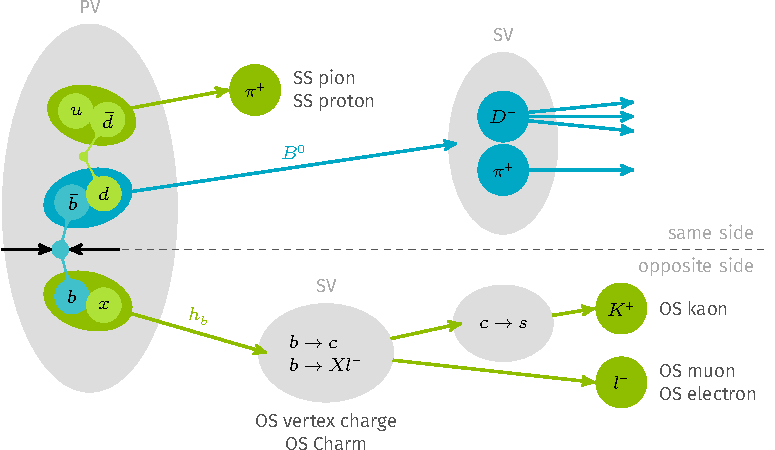
\includegraphics[width=0.8\textwidth]{08FlavourTagging/figs/FTscheme.pdf}
    \caption{Schematic overview of all available \Bz tagging algorithms.}
    \label{fig:taggingalgorithms}
\end{figure}
They can be separated into so-called opposite side (OS) and same side (SS) algorithms.

The OS algorithms exploit the production and decay of the second \bquark-quark which is produced in the proton-proton collision.
By partially reconstructing single decay products as electrons, muons, kaons and \D-mesons associated with the decay of the opposite side \bquark-hadron the initial flavour is inferred.
Furthermore, charged tracks which originate from a secondary vertex, which is displaced from the \ac{PV}, are used to make a decision on the production flavour of the signal $B$-meson.
As the hadronisation and the decay of the OS \bquark-hadron is independent of the signal \B-meson these algorithms can be used for both \Bz and \Bs mesons. Based on \cite{LHCb-PAPER-2011-027, LHCb-PAPER-2015-027} the OS algorithms are briefly described below:
\begin{itemize}
	\item The OS muon and OS electron tagger use the charge of muons and electrons from semileptonic $\bquark\!\to Xl^-$ decays to take a decision on the initial $B$-flavour.
	The charged leptons are selected using a simple cut-based selection.
	To suppress contributions from $\bquark\!\to\cquark\!\to l^+$ decays, which would give the wrong tag decision, for example the transverse momentum of the muon (electron) is required to be larger than \SI[per-mode=symbol]{1.2}{\GeVc} (\SI[per-mode=symbol]{1.0}{\GeVc}).
	Electrons have additionally to satisfy criteria on electron identification variables such as the ratio $\nicefrac{E}{p}>0.8$.
	Here $E$ denotes the energy deposited in the ECAL and $p$ the electron momentum.
	If more than one muon or electron per event survives the selection, the lepton with the highest transverse momentum is chosen to define the flavour of the signal $B$.
	The mistag is estimated with an artificial neural network, which takes as inputs event properties as the number of \ac{PV}s and tracks in the event, $B$-properties as the transverse momentum and various geometrical and kinematic properties of the tagging lepton.
	\item The OS kaon tagger explores the charge of kaons produced in the decay chain $\bquark\!\to\cquark\!\to\squark$.
	Very similar to the lepton taggers the tagging kaon is selected using rectangular cuts based on kinematic and PID observables.
	In case multiple kaons per event pass this selection, the kaon with the highest transverse momentum is fed into an artificial neural network with similar inputs as for the lepton taggers to calculate the mistag estimate $\eta$.
	\item The OS charm tagger selects \D-mesons produced via $\bquark\!\to\cquark$ decays.
	In case of a charged \D-meson the charge of the meson directly hints at the initial flavour, in case of an uncharged \D-meson the charge of the produced kaon is used to infer the flavour of the signal $B$-meson.
	In contrast to the other single track taggers a \ac{BDT} is used to select the \D-meson and estimate the mistag.
	As the OS charm is the newest development on the OS it was developed to have a small overlap concerning the used tagging particles with the other taggers.
	\item The OS vertex charge tagger is the only algorithm which does not reconstruct single particles, but uses the weighted charge of a \ac{SV} associated with the opposite side \bquark-hadron instead.
	In order to do this, the track pair with the highest probability of originating from the opposite side \bquark-hadron is used to build a vertex.
	Following, particles which are compatible with coming from this two-track vertex but not from the \ac{PV} are added to it.
	Finally all tracks of the final \ac{SV} are weighted with their transverse momentum, \pt, and used to calculate a charge
	\begin{equation}
	Q_{\text{vtx}}=\frac{\sum_{i}p_{\mathrm T}^k(i)Q_i}{\sum_{i}p_{\mathrm T}^k(i)}
	\end{equation}
	where the parameter $k$ is optimised to maximise the performance of the tagging algorithm.
	Based on this charge the initial flavour of the signal $B$-meson is then determined.
\end{itemize}

The SS algorithms use remnants of the hadronisation of the signal \B-meson to infer the initial flavour.
As the companion quark of the \bquark-quark is different for \Bz and \Bs-mesons, different algorithms must be used to deduce the initial flavour of the signal \B.

In case of a \Bz (\bquarkbar\dquark) a free \dquarkbar-quark is produced which can hadronise to a pion or proton.
Additionally, the production mechanisms, \eg via the strong decay of an excited $B^{**+}\!\to B^{(*)0}\pip$ can be exploited~\cite{Aaij:2016rdg}.
The SS pion and SS proton taggers use the charge of these companion particles to infer a tag decision.
They were developed on \BdToDpi decays assuming $\Sf=\Sfbar=0$, \ie the decay \BdToDpi is \CP-conserving.
Therefore a potential bias of the analysis cannot be excluded when using these algorithms and they are retrained on $\Bz\!\to\jpsi\Kstarz$.
The basic strategy is similar to the one in Ref.~\cite{Aaij:2016rdg}:
First, tagging particles from the same region of phase space as the signal \B are selected using requirements on PID, kinematic and geometrical observables.
Then, these particles are all used to train a \ac{BDT}, which further selects the final tagging particle and estimates the mistag.
This means in case multiple particles per event pass the selection, the SS pion and SS proton taggers do not select the particle with highest transverse momentum but for all particles the \ac{BDT} response is calculated and the tagging candidate with the largest \ac{BDT} response is chosen afterwards to infer the initial flavour of the signal \B.

On the other hand the hadronisation of a \Bs (\bquarkbar\squark) leads to a \squarkbar-quark which can hadronise to a kaon~\cite{Aaij:2016psi}.
The SS kaon tagger was developed to identify such kaons and works similar for kaons as the SS pion tagger for pions produced in \Bz events.
Since this analysis covers decays of neutral \Bz mesons and the SS kaon tagger is not used, this algorithm is not discussed any further.

\subsection{Performance characteristics}

The predictions of the flavour tagging algorithms are not perfect.
Of $N$ reconstructed candidates only $N'$ candidates get a tag $d$ and mistag $\eta$ assigned, while $N_{\text{U}}$ are untagged.
The $N'$ candidates can be further divided into $N_{\text{W}}$ candidates which are wrongly tagged and $N_{\text{R}}$ correctly tagged candidates.
These imperfections can be reflected by a tagging efficiency
\begin{equation}
\varepsilon_{\text{tag}}=\frac{N_{\text{R}}+N_{\text{W}}}{N_{\text{R}}+N_{\text{W}}+N_{\text{R}}+N_{\text{U}}}\label{eq:tageff}
\end{equation}
and a mistag probability
\begin{equation}
\omega=\frac{N_{\text{W}}}{N_{\text{R}}+N_{\text{W}}}\,.\label{eq:mistag}
\end{equation}
Therefore, in an analysis using flavour tagging to infer the initial \B flavour the number $N_{\Bz}(t)$ ($N_{\Bzb}(t)$) of measured initial \Bz (\Bzb) candidates are
\begin{equation}
\begin{aligned}
N_{\Bz}(t)&=(1-\omega)N_{\Bz}^{\text{true}}(t)+\omega N_{\Bzb}^{\text{true}}(t)\,,\\
N_{\Bzb}(t)&=\omega N_{\Bz}^{\text{true}}(t)+(1-\omega)N_{\Bzb}^{\text{true}}(t)
\end{aligned}
\end{equation}
where $N_{\B}^{\text{true}}$ denotes the true number of initial \Bz and \Bzb candidates.
These quantities need to be transferred further into measurements of \CP-asymmetries such as
\begin{equation}
A_{\CP}(t)=\frac{N_{\Bz}^{\text{true}}(t)-N_{\Bzb}^{\text{true}}(t)}{N_{\Bz}^{\text{true}}(t)+N_{\Bzb}^{\text{true}}(t)}\,.
\end{equation}
For a measured asymmetry the true numbers of initial \Bz- and \Bzb-mesons need to be replaced with the observed yields which leads to
\begin{equation}
A_{\CP}^{\text{meas}}(t)=\frac{N_{\Bz}(t)-N_{\Bzb}(t)}{N_{\Bz}(t)+N_{\Bzb}(t)}=(1-2\omega)A_{\CP}^{\text{theo}}(t)
\end{equation}
with the dilution $D=1-2\omega$.
However, experimentally not only the dilution affects the measured asymmetry but also intrinsic asymmetries $I$ like an asymmetric production of \Bz- and \Bzb-mesons might influence a measurement so that the measured asymmetry can be expressed as
\begin{equation}
A_{\CP}^{\text{meas}}(t)=DA_{\CP}(t)+I\,.
\end{equation}
As the mistag probability is defined in the range $[0, 0.5]$ the dilution can take values between \num{0} and \num{1}.
A large dilution factor is equivalent to a vanishing mistag and hence leads to a larger experimental sensitivity as will be shown below.
To simplify the following discussion the intrinsic asymmetries and dilution are assumed to be time-independent, even if that is not generally valid.
The theoretical asymmetry can then be expressed as
\begin{equation}
A_{\CP}(t)=\frac{1}{D}\left(A_{\CP}^{\text{meas}}(t)-I\right)\,.
\end{equation}
Assuming that all quantities are uncorrelated and gaussian distributed the uncertainty on the theoretical asymmetry is given by
\begin{equation}
\begin{aligned}
\sigma_{A_{\CP}}^2&=\left(\frac{\partial A_{\CP}}{\partial N_{\Bz}}\right)^2\sigma_{N_{\Bz}}^2+\left(\frac{\partial A_{\CP}}{\partial N_{\Bzb}}\right)^2\sigma_{N_{\Bzb}}^2+\left(\frac{\partial A_{\CP}}{\partial I}\right)^2\sigma_{I}^2+\left(\frac{\partial A_{\CP}}{\partial D}\right)^2\sigma_{D}^2\\
&=\frac{1}{D^2}\frac{1}{N_{\Bz}(t)+N_{\Bzb}(t)}\left(1-A_{\CP}^{\text{meas}}(t)\right)+\frac{\sigma_{I}^2}{D^2}+\frac{A_{\CP}^2(t)}{D^2}\sigma_{D}^2\,.
\end{aligned}
\end{equation}
Neglecting the uncertainties on the intrinsic asymmetries and dilution factor and further assuming that the measured asymmetries are small, this expression can be reduced to
\begin{equation}
\sigma_{A_{\CP}}^2=\frac{1}{D^2}\frac{1}{N_{\Bz}(t)+N_{\Bzb}(t)}\,.
\end{equation}
Here it is useful to identify the number of measured \Bz- and \Bzb-candidates as
\begin{equation}
N_{\Bz}(t)+N_{\Bzb}(t)=\varepsilon(t)N
\end{equation}
where $\varepsilon$ includes all efficiencies either in the trigger, reconstruction, selection or the flavour tagging.
Regarding the flavour tagging this means that the uncertainty on a \CP-asymmetry is given by
\begin{equation}
\sigma_{A_{\CP}}=\frac{1}{\sqrt{\varepsilon_{\text{tag}}D^2N}}=\frac{1}{\sqrt{\varepsilon_{\text{eff}}N}}
\end{equation}
where the effective tagging efficiency $\varepsilon_{\text{eff}}=\varepsilon_{\text{tag}}D^2$ was introduced.
As one can see, this efficiency defines the experimental sensitivity of the measurement as it effectively reduces the number of candidates.
It also becomes obvious that the tagging efficiency introduced in \cref{eq:tageff} and the mistag probability defined in \cref{eq:mistag} are not individually suitable for determining the performance of different tagging algorithms.
Instead the tagging efficiency, which is also denoted as tagging power, must be used.

Rather than using an average mistag $\omega$ the mistag estimate $\eta$ of the various tagging algorithms can be used.
To do this, the estimated mistag has to be calibrated with a calibration function $\omega(\eta)$ (more details on the calibration are given in \cref{sec:CombAndCalib}), what gives a per-event tagging power, defined as
\begin{equation}
\varepsilon_{\text{eff}}=\frac{1}{N}\sum_{i=1}^{N}D_i^2=\frac{1}{N}\sum_{i=1}^{N}\left(1-2\omega(\eta_i)\right)^2\,.
\end{equation}
Here the sum is iterating over all candidates and for untagged candidates the mistag probability is defined to be \num{0.5} ($D_i=0$).

When considering only tagged candidates, the effective tagging efficiency reduces to a pseudo tagging power, which is effectively the same as average of the dilution squared in the respective sample:
\begin{equation}
\left<D^2\right>=\frac{1}{N_{\text{R}}+N_{\text{W}}}\sum_{i=1}^{N_{\text{R}}+N_{\text{W}}}\left(1-2\omega(\eta_i)\right)^2\,.
\end{equation}

\subsection{Combination and calibration of flavour tagging algorithms}
\label{sec:CombAndCalib}

To improve the overall performance of the flavour tagging the individual algorithms are combined to form one single tag decision and mistag for the OS ($d_{\text{OS}}$ and $\eta_{\text{OS}}$) and a tag decision and mistag for the SS ($d_{\text{SS}}$ and $\eta_{\text{SS}}$).
This is done by calculating the combined probability, that a \B-candidate contains a \bquark-quark
\begin{equation}
P(\bquark)=\frac{p(\bquark)}{p(\bquark)+p(\bquarkbar)}\hspace{0.5cm}\text{and}\hspace{0.5cm}P(\bquarkbar)=1-P(\bquark)\,.
\end{equation}
The probabilities $p(\bquark)$ and $p(\bquarkbar)$ are defined as
\begin{equation}
p(\bquark)=\prod_{i}\left(\frac{1+d_i}{2}-d_i\left(1-\eta_i\right)\right)
\end{equation}
and
\begin{equation}
p(\bquarkbar)=\prod_{i}\left(\frac{1-d_i}{2}+d_i\left(1-\eta_i\right)\right)
\end{equation}
where $d_i$ ($\eta_i$) are the tag decisions (mistag estimates) of the individual tagging algorithms.
The combined tag decision and mistag are now defined as $d=-1$ and $\eta=1-P(\bquark)$ if $P(\bquark)>P(\bquarkbar)$ and as $d=+1$ and $\eta=P(\bquark)$ if $P(\bquark)<P(\bquarkbar)$.

As mentioned before, the output of the flavour tagging algorithms is mostly the result of multivariate classifiers, which are trained on flavour specific \B decays.
This output is then transformed into a mistag estimate $\eta$ and crosschecked on another flavour specific validation sample.
However, the training and validation sample are usually different from the signal decay used in a \CP-violation measurement.
This differences are caused by different trigger and selection criteria and can influence the distributions which are used by the multivariate classifier to estimate the mistag.
Consequently, the mistag must be calibrated on a dedicated flavour specific decay, which shows at best kinematically similar distributions compared to the signal decay.
For the OS taggers this is most often done using charged decay modes, as the charge of the final state particles allows to directly infer the production flavour.
Instead, to calibrate the SS taggers a decay mode with the same initial \B flavour is needed, as these taggers highly depend on the hadronisation process.
In this analysis the OS taggers are calibrated using $\Bu\!\to\Dz\pip$, where the bachelor pion allows to infer the initial flavour, while the SS taggers are calibrated using $\Bz\!\to\jpsi\Kstarz$.

So far, for all analyses at \lhcb a linear calibration function of the form
\begin{equation}
\omega(\eta)=\tilde{p}_0+\tilde{p}_1\left(\eta-\left<\eta\right>\right)\label{eq:linCalib}
\end{equation}
where the arithmetic mean $\left<\eta\right>$ of the estimated mistag is used to decorrelate the calibration parameters $p_0$ and $p_1$, was sufficient.
Using this calibration function a perfect calibration, \ie $\omega=\eta$, would result in $\tilde{p}_0=\left<\eta\right>$ and $\tilde{p}_1=1$.
Yet, the performance of the tagger can depend on the initial \B flavour:
If the interaction rates of charged decay products (\eg the kaons used by the OS kaon tagger) with the detector material depend on the charge, the mistags will also depend on the flavour of the initial \B meson.
Such asymmetry yields in an additional dilution factor, which needs to be understood and properly described.
This can be achieved by using different calibration functions for \Bz- and \Bzb-mesons.
In the simple linear case these calibration functions are
\begin{equation}
\begin{aligned}
\omega&=p_0+p_1+\left(\eta-\left<\eta\right>\right)\,,\\
\overline{\omega}&=\overline{p}_0+\overline{p}_1+\left(\eta-\left<\eta\right>\right)\,.
\end{aligned}
\end{equation}
These different calibration parameters are furthermore linked to each other via the average calibration parameters $\tilde{p}_i$ used in \cref{eq:linCalib} and corresponding differences $\Delta p_i$ defined as
\begin{equation}
\tilde{p}_i=\frac{p_i+\overline{p}_i}{2}\hspace{0.5cm}\text{and}\hspace{0.5cm}\Delta p_i=p_i-\overline{p}_i\,\,.
\end{equation}

However, due to the large number of \BdToDpi signal candidates small effects that were hidden in the statistical uncertainties before become significant.
Therefore more sophisticated calibration functions are needed to calibrate the flavour tagging algorithms.
The adopted models are called generalised linear models (GLM)~\cite{GLM} and have the following form:
\begin{equation}
\WorWbar(\eta) = g\left(h(\eta)\right) = g\left( g^{-1} (\eta) + \sum_{i=1}^{N} \left(\tilde{p}_i \kern 0.0em\optbar{\kern -0.0em +} \frac{\Delta p_i}{2}\right) f_i(\eta)\right)\,.
\end{equation}
The functions $f_i$ are the so-called \emph{basis functions}, which for example can be simple poynomials or natural spline functions~\cite{Nsplines}.
To minimise the correlation between the $\tilde{p}_i$ and $\Delta p_i$ parameters the \emph{basis functions} are orthogonalised using the Gram-Schmidt method~\cite{GramSchmidt}.
The function $g$ is referred to as \emph{link function}, which is usually defined as the inverse cumulative distribution function, to map all input values to the range $[0,1]$, \ie an interval which can be interpreted as a probability.
As the mistag is only defined in the range $[0, 0.5]$ it is possible, that after applying a calibration function with this \emph{link function} the mistag is larger than \num{0.5}.
In this case an arbitrary decision has to be taken how such candidates are further treated.
Possible options are to either flip the corresponding tag decision $d\to-d$ and adjust the mistag $\omega\to1-\omega$ or to mark the candidate as untagged with a mistag of \num{0.5}.
The latter possibility leads to fit instabilities in the decay-time fit when the calibration parameters are not fixed, but allowed to float or constrained by means of a Gaussian function.
This is due to the fact that for a floating or constrained calibration the ratio of tagged and untagged candidates varies during the minimisation and the changes to the likelihood are not continous.
On the other hand, a flip of the tagdesicion may yield in a bias of the \CP-parameters as shown in \cref{sec:ValLinkFunction}.
Therefore, the modified logistic function
\begin{equation}
g(h)=\frac{1}{2\left(1+e^h\right)}\label{eq:modlink}
\end{equation}
is used as \emph{link function}, which maps all input values into the range $[0, 0.5]$ and hence assures that all calibrated mistags are well defined.

To not rely on possible binning effects on the estimated mistag $\eta$ or the mistag probability $\omega$, the calibration functions are determined using an unbinned maximum-likelihood method, the so-called binomial regression~\cite{BinRegression}.

\section{Flavour tagging strategy}
\label{sec:taggingstrategy}

In this analysis the combination of all available OS algorithms is used, while for the SS both taggers designed to infer the initial flavour of \Bz-mesons are combined into one single tag decision and mistag.
The OS taggers were all developed and trained on a datasample of $\Bu\!\to\jpsi\Kp$ decays, except for the OS charm tagger, whose BDT was trained on a mixed sample of simulated $\Bu\!\to\jpsi\Kp$, $\Bz\!\to\jpsi\Kstarz$ and $\Bs\!\to\jpsi\phi$ decays.
As the OS taggers are independent of the initial signal \B they can be used in this default version.
As control channel the decay $\Bu\!\to\Dz\pip$ is used.
As mentioned before, the SS pion and the SS proton taggers were deveolped and trained on a datasample of \BdToDpi decays, assuming no \CP-violation.
The use of these algorithms could therefore bias the measurement of \Sf and \Sfbar and hence both taggers are retrained (more details given in \cref{sec:retrainSSpion} and \cref{sec:retrainSSproton}).

To include the flavour tagging in the decay rates given in \crefrange{eq:DecRateB2Dmpip}{eq:DecRateBb2Dppim} the expressions for the \CP-parameters \Sf and \Cf need to be extended to
\begin{equation}
\begin{aligned}
\Sf&\to\left(\Delta^--\Delta^+\right)\Sf\,\,,\\
\Cf&\to\left(\Delta^--\Delta^+\right)\Cf\,\,.\label{eq:decRateCorrectFT}
\end{aligned}
\end{equation}
Similar equations hold also for \Sfbar and \Cfbar.
The coefficients $\Delta^\pm$ contain the calibration functions and tagging efficiencies $\varepsilon_{\text{tag}}^{\text{OS}}$ and $\varepsilon_{\text{tag}}^{\text{SS}}$.
They are defined as
\begin{align}
\Delta^\pm&=\frac{1}{2}\varepsilon_{\text{\tiny tag}}^{\text{\tiny OS}}\left[1-\varepsilon_{\text{\tiny tag}}^{\text{\tiny SS}}+d^{\text{\tiny OS}}\left(1-\varepsilon_{\text{\tiny tag}}^{\text{\tiny SS}}-2\omega(\eta^{\text{\tiny OS}})\left(1+\varepsilon_{\text{\tiny tag}}^{\text{\tiny SS}}\right)\right)\right]\nonumber\\
&\pm\frac{1}{2}\varepsilon_{\text{\tiny tag}}^{\text{\tiny OS}}\left[1-\varepsilon_{\text{\tiny tag}}^{\text{\tiny SS}}+d^{\text{\tiny OS}}\left(1-\varepsilon_{\text{\tiny tag}}^{\text{\tiny SS}}-2\overline{\omega}(\eta^{\text{\tiny OS}})\left(1+\varepsilon_{\text{\tiny tag}}^{\text{\tiny SS}}\right)\right)\right]
\end{align}
for candidates which are only tagged by the OS tagger combination.
To obtain the expression for candidates only tagged by the SS taggers, all superscripts need to be exchanged with $\text{OS}\leftrightarrow\text{SS}$.
For candidates which are tagged by both, the OS tagger combination and the SS taggers the coefficients can be written as
\begin{align}
\Delta^\pm&=\frac{1}{4}\varepsilon_{\text{\tiny tag}}^{\text{\tiny OS}}\varepsilon_{\text{\tiny tag}}^{\text{\tiny SS}}\left[1+\hspace{-3mm}\sum_{j=\text{\tiny OS, SS}}\hspace{-2mm}d_j\left(1-2\omega(\eta_j)\right)+d^{\text{\tiny OS}}d^{\text{\tiny SS}}\left(1-2\omega(\eta_j)+2\omega(\eta^{\text{\tiny OS}})\omega(\eta^{\text{\tiny SS}})\right)\right]\nonumber\\
&\pm\frac{1}{4}\varepsilon_{\text{\tiny tag}}^{\text{\tiny OS}}\varepsilon_{\text{\tiny tag}}^{\text{\tiny SS}}\left[1+\hspace{-3mm}\sum_{j=\text{\tiny OS, SS}}\hspace{-2mm}d_j\left(1-2\overline{\omega}(\eta_j)\right)+d^{\text{\tiny OS}}d^{\text{\tiny SS}}\left(1-2\overline{\omega}(\eta_j)+2\overline{\omega}(\eta^{\text{\tiny OS}})\overline{\omega}(\eta^{\text{\tiny SS}})\right)\right]\,.
\end{align}

The flavour specific control samples ($\Bu\!\to\Dz\pip$ for the OS, $\Bz\!\to\jpsi\Kstarz$ for the SS) are used to determine the functional form of the calibration function $\omega(\eta)$.
Unlike other flavour tagged analyses at \lhcb the calibration parameters can be determined directly in the decay-time fit as floating nuisance parameter of the likelihood function in \BdToDpi.
This is possible because the parameters \Cf and \Cfbar are fixed to \num{1} and \num{-1} as the ratio $r$ (see \cref{eq:ratioDpi}) is expected to be too small to allow a significant measurement of both parameters.
As a result, the cosine term allows to determine the calibration parameters independently of the sine term.
A qualitative explanation of this is given in \cref{fig:FTstrategy}.
\begin{figure}[tbp]
    \centering
    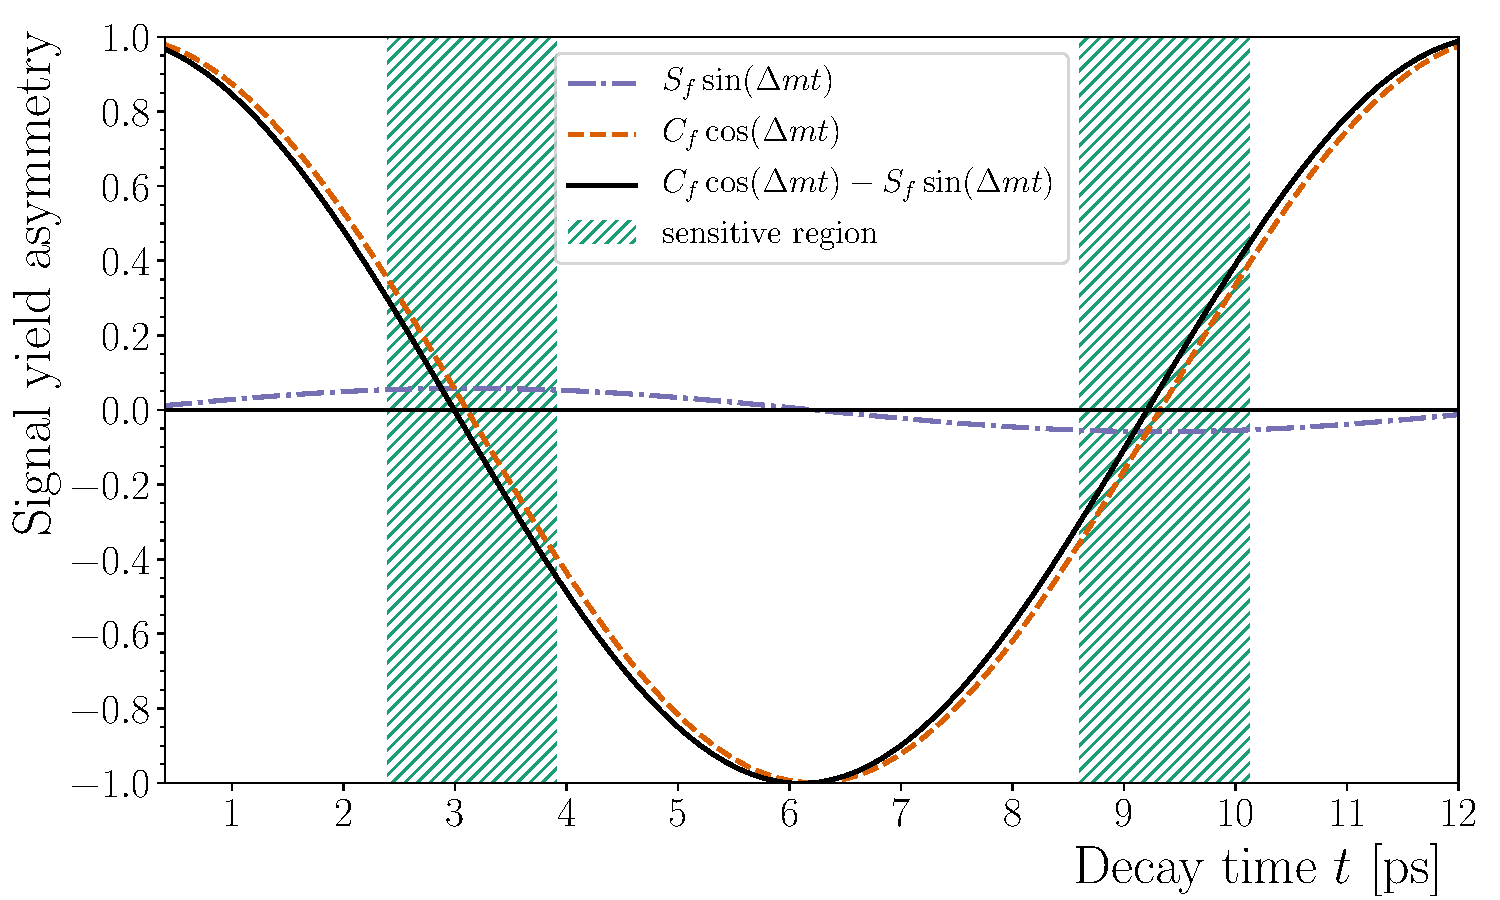
\includegraphics[width=0.48\textwidth]{08FlavourTagging/figs/oscillation_f.pdf}
    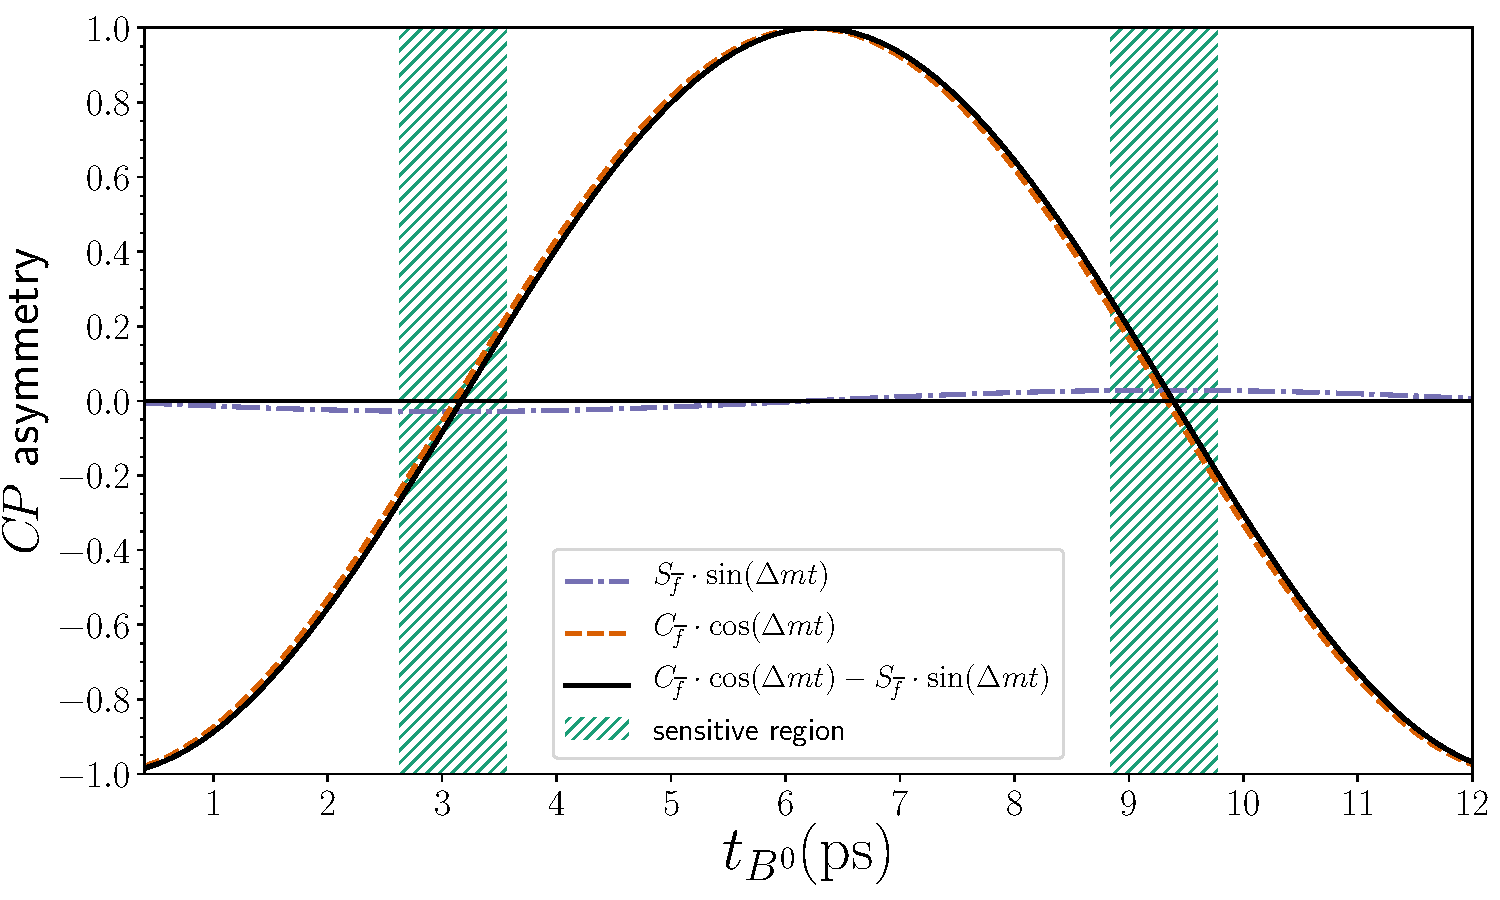
\includegraphics[width=0.48\textwidth]{08FlavourTagging/figs/oscillation_fbar.pdf}
    \caption{Time-dependent asymmetries for \Bzb versus \Bz for the \Dm\pip (left) and \Dp\pim (right) final states.
    The values for the \CP parameters are taken from simulation and no experimental dilutions are included.
    Since the deviation of the sum of both trigonometric functions from a single cosine function is very small due to the tiny values of \Sf and \Sfbar, the maximum sensitivity is achieved in the regions of the zero-points, \ie where the amplitude of $\cos(\dm t)$ and $\sin(\dm t)$ are of similar size.
    These regions are denoted as \enquote{sensitive regions} in both plots.
    In the \enquote{non-sensitive regions}, where the cosine-function is completely dominating, additional diluting effects due to the tagging calibration can be determined.}
    \label{fig:FTstrategy}
\end{figure}

When determining all calibration parameters directly in the signal sample no assumptions for the portability of the calibration from a control channel is needed.
This portability in principle can be limited due to kinematic differences between the control sample and the signal sample leading to different flavour tagging calibrations.
It is probed using simulated events of both, the control sample and the signal sample.
When checking the portability of the calibrations from $\Bu\!\to\Dz\pip$ and $\Bz\!\to\jpsi\Kstarz$ to \BdToDpi a bias on \Sf and \Sfbar of roughly the size of their statistical uncertainty arises.
This bias can be reduced when floating the calibration parameters (more details on this are given in \cref{sec:decTimeFitVal}).
Furthermore, the precision of the calibration parameters for the SS tagger combination obtained in the decay-time fit to \mbox{\BdToDpi} is much smaller compared to the precision on the control channel, while for the OS tagger combination the uncertainty on the signal sample increases only slightly compared to the uncertainty obtained on the control sample.
However, determining the calibration parameters in the final decay-time fit leads to an increased statistical uncertainty on the \CP-parameters \Sf and \Sfbar due to the additional degrees of freedom in the fit.
This is compensated by the fact that the systematic uncertainty for the portability of the calibration, which is often the largest systematic uncertainty for flavour tagged analyses at \lhcb, is not needed.

A quantitative validation of this strategy was done by a collaborator on pseudoexperiments:
Generating pseudoexperiments and floating the parameters \Cf and \Cfbar in the fit showed a non-negligible bias for the parameters \Sf and \Sfbar, while fixing the coefficients \Cf and \Cfbar in the fit showed unbiased results on all fitted parameters.
Therefore this strategy is adopted for the extraction of the calibration parameters.
Finally it should be noted here that possible deviations from the assumption of $\Cf=-\Cfbar=1$ are taken into account in the systematic uncertainties (\cref{ch:systeamticUncerts}).

Thus, the studies presented in the following sections do not aim to obtain the calibration parameters.
Instead, on the one hand, they are used to determine the functional form of the calibration function, which is used in the decay-time fit described in \cref{sec:ExtractCPobs}.
On the other hand, the obtained parameter values of the calibration function can be used as reference values for the decay-time fit, as even if they are not expected to agree perfectly, both parameter sets should be in the same interval.

\section{Same side tagging calibration}
\label{sec:SScalibration}

The SS tagger combination is retrained and calibrated on the datasample of $\Bz\!\to\jpsi\Kstarz$ candidates corresponding to \SI{3}{\per\femto\barn}, recorded in \num{2011} and \num{2012} at centre-of-mass energies of \SI{7}{\tera\electronvolt} and \SI{8}{\tera\electronvolt}, respectively.
It is used because $\Bz\!\to\jpsi\Kstarz$ is the only flavour-specific decay mode of \Bz-mesons with a sufficient large statistic beside the signal mode of \BdToDpi at \lhcb.
The strategy follows mainly the one which was used to train the original taggers on \BdToDpi what is described in Ref.~\cite{Aaij:2016rdg}.
Only one additional step is implemented:
The distributions of $\Bz\!\to\jpsi\Kstarz$ candidates are kinematically weighted to match the distributions of \BdToDpi candidates.
The general procedure is quite similar for both tagging algorithms and looks as following:
\begin{itemize}
	\item The $\Bz\!\to\jpsi\Kstarz$ sample is selected and a fit to the invariant mass is performed, in order to separate the signal and background components statistically.
	Using the \emph{sPlot} method weights are calculated, which allow to obtain the signal-component distributions of other variables. This is reported in \cref{sec:PrepBd2JpsiKstSample}
	\item The distributions of transverse momentum \pt, pseudo-rapidity $\eta'$ and azimuthal angle $\phi$ of the \Bz candidate, the number of tracks and the number of \ac{PV}s in the event and a distribution of Hlt2 trigger decisions for $\Bz\!\to\jpsi\Kstarz$ candidates are weighted to match those of the \BdToDpi candidates.
	This has two reasons: First the performance of the BDT is potentially improved when applying to \BdToDpi, second the portability of the functional form of the calibration is assured, and calibration parameters obtained can be better used as reference values.
	\item The tagging particles, whose charge is correlated with the initial \B flavour are selected
	\item Finally the datasample is divided into three subsamples:
	\begin{itemize}
		\item The first third of the sample is used to train a BDT to separate correctly and wrongly charged tagging particles.
		Hereby correctly tagged means that the charge of the tagging particle would indicate the correct tag, while wrongly tagged denotes exactly the opposite situation: The tagging particles' charge would indicate the wrong tag decision.
		To reduce the number of oscillated \Bz-mesons only \Bz-mesons with a decay time smaller than the first maximum of the oscillation are used.
		Therefore, following the procedure in Ref.~\cite{Aaij:2016rdg}, \Bz-mesons used in the training are required to have a a decay time smaller than \SI{2.2}{\pico\second}.
		\item On the second subsample the BDT is tested in order to avoid effects as overtraining.
		Furthermore, both, the first training sample and this second testing sample are used to determine the mistag as a function of the BDT response. For this latter step the requirement on the \Bz decay time is removed, as a full time-dependent analysis of the \Bz oscillation is performed.
		\item Finally on the last third the SS taggers are combined and the functional form of the calibration is determined together with reference values for the calibration parameters obtained in the decay-time fit described in \cref{sec:ExtractCPobs}.
	\end{itemize}
\end{itemize}

\subsection[head={Preparation of the $\Bz\!\to\jpsi\Kstarz$ samples},tocentry={Preparation of the $\Bz\!\to\jpsi\Kstarz$ samples}]{Preparation of the $\symbfsf{\Bz\!\to\jpsi\Kstarz}$ samples}
\label{sec:PrepBd2JpsiKstSample}


The decay $\Bz\!\to\jpsi\Kstarz$ is reconstructed using the decays $\jpsi\!\to\mup\mun$ and \mbox{$\Kstarz\!\to\Kp\pim$}.
The cuts applied in the stripping are listed in \cref{tab:JpsiKstStripping}.
Again, to achieve  better compatibility between $\Bz\!\to\jpsi\Kstarz$ and the signal decay \BdToDpi, the same trigger requirements as for the signal mode are applied.
After the trigger requirements the \Kstarz- and the \jpsi-meson are requried to fulfill the cuts shown in \cref{tab:selJpsiKst}.
\begin{table}[tbp]
	\centering
	\caption{Stripping cuts for the decay $\Bz\!\to\jpsi\Kstarz$ with $\jpsi\!\to\mup\mun$ and $\Kstarz\!\to\Kp\pim$.
	For the charged tracks the more stringent requirements for the bachelor track are given in brackets.
	For the impact parameter the shortcut IP is used, DOCA denotes the distance of closest approach of the respective \Kstarz or \jpsi mesons and $m_{p^+p^-}$ denotes the invariant mass of the \mup\mun or \Kp\pim combination.}
	\begin{tabular}{ccc}
		\toprule
		\multicolumn{3}{c}{\muon requirements}\\
		\midrule
		transverse momentum \pt 	& \multicolumn{2}{c}{$>\SI[per-mode=symbol]{500}{\MeVc}$} \\
		\dllmupi					& \multicolumn{2}{c}{$>0.0$} \\
		\midrule
		resonances-requirements & \jpsi & \Kstarz\\
		\midrule
		transverse momentum \pt 							& - 								& $>\SI[per-mode=symbol]{500}{\MeVc}$ \\
		DOCA $\chi^2$										& $<20.0$ 							& $<30.0$ \\
		$\left|m_{p^+p^-}-m_{\jpsi}^{\text{PDG}}\right|$	& \SI[per-mode=symbol]{150}{\MeVcc} & \SI[per-mode=symbol]{300}{\MeVcc} \\
		decay vertex $\chi^2$ 								& $<16.0$ 							& $<25.0$ \\
		\midrule
		\multicolumn{3}{c}{\Bz-meson requirements}\\
		\midrule
		reconstructed decay time $t$ 	& \multicolumn{2}{c}{$>\SI{0.2}{\pico\second}$} \\
		\bottomrule
	\end{tabular}
	\label{tab:JpsiKstStripping}
\end{table}
\begin{table}[tbp]
	\centering
	\caption{Cuts to select $\Bz\!\to\jpsi\Kstarz$ candidates.
	The transverse momentum is denoted as \pt, for the impact parameter the shortcut IP is used and $h$ denotes a kaon or pion.}
	\begin{tabular}{cc}
		\toprule
		\jpsi/\muon requirements & \Kstarz/(\kaon, \pion) requirements\\
		\midrule
		$\dllmupi>0$																& $\dllkpi>0$ \hspace{0,2cm} for kaons \\
		track $\nicefrac{\chi^2}{\text{ndof}}<4$ 									& track $\nicefrac{\chi^2}{\text{ndof}}<4$ \\
		$\pt(\mup)>\SI{500}{\MeVc}||\pt(\mun)>\SI[per-mode=symbol]{500}{\MeVc}$ 	& $\pt(\Kstarz)>\SI[per-mode=symbol]{1000}{\MeVc}$\\
		vertex $\chi^2$/ndof$<16$ of \jpsi 											& vertex $\chi^2$/ndof$<16$ of \Kstarz\\
		$\left|m_{J/\psi}-m_\text{PDG}\right|<\SI[per-mode=symbol]{80}{\MeVcc}$ 	& $\left|m_{\Kstarz}-m^\text{PDG}\right|<\SI[per-mode=symbol]{70}{\MeVcc}$\\
		\bottomrule
	\end{tabular}
	\label{tab:selJpsiKst}
\end{table}
Additionally only \Bz-candidates with an invariant mass within the range $[5100, 5450]\,$\si[per-mode=symbol]{\MeVcc}, a transverse momentum larger than \SI{1}{\GeVc}, the minimal $\chi^2$ of the impact parameter w.r.t. the \ac{PV} smaller than \num{25} and $\nicefrac{\chi^2}{\text{ndof}}$ of the decay vertex smaller than ten are selected.
Last the DTF $\nicefrac{\chi^2}{\text{ndof}}$ is required to be smaller than five and the number of \ac{PV}s in the event has to be one, or in case an event has more than one \ac{PV} the impact parameter $\chi^2$ has to be larger than \num{50}.
In case of multiple \Bz candidates the one with the smallest DTF $\nicefrac{\chi^2}{\text{ndof}}$ is chosen.

To extract \emph{sWeights} a fit to the invariant \Bz mass, stemming from the DTF with a constraint on the known \jpsi mass is performed.
The signal model consists of a sum of two double-sided Hypatia functions with a shared mean value, the background is parametrised using an exponential function.
The first Hypatia function describes mainly $\Bz\!\to\jpsi\Kstarz$ candidates without photon radiation in the final state, while the second Hypatia shows a large tail towards smaller invariant masses.
The tail parameters $a_i$ and $n_i$ of both Hypatia functions are determined on simulated events.
Moreover the fraction between both signal components and the parameter $\lambda$ of the Hypatia describing the \Bz candidates with harder photon radiation are taken from fits to simulated samples.
All remaining parameters are floating.
The fit which is performed in the range $[5200, 5350]\,$\si[per-mode=symbol]{\MeVcc} is shown in \cref{fig:massFitJpsiKst} and the resulting yields are given in \cref{tab:yieldsJpsiKst}.
\begin{figure}[tbp]
    \centering
    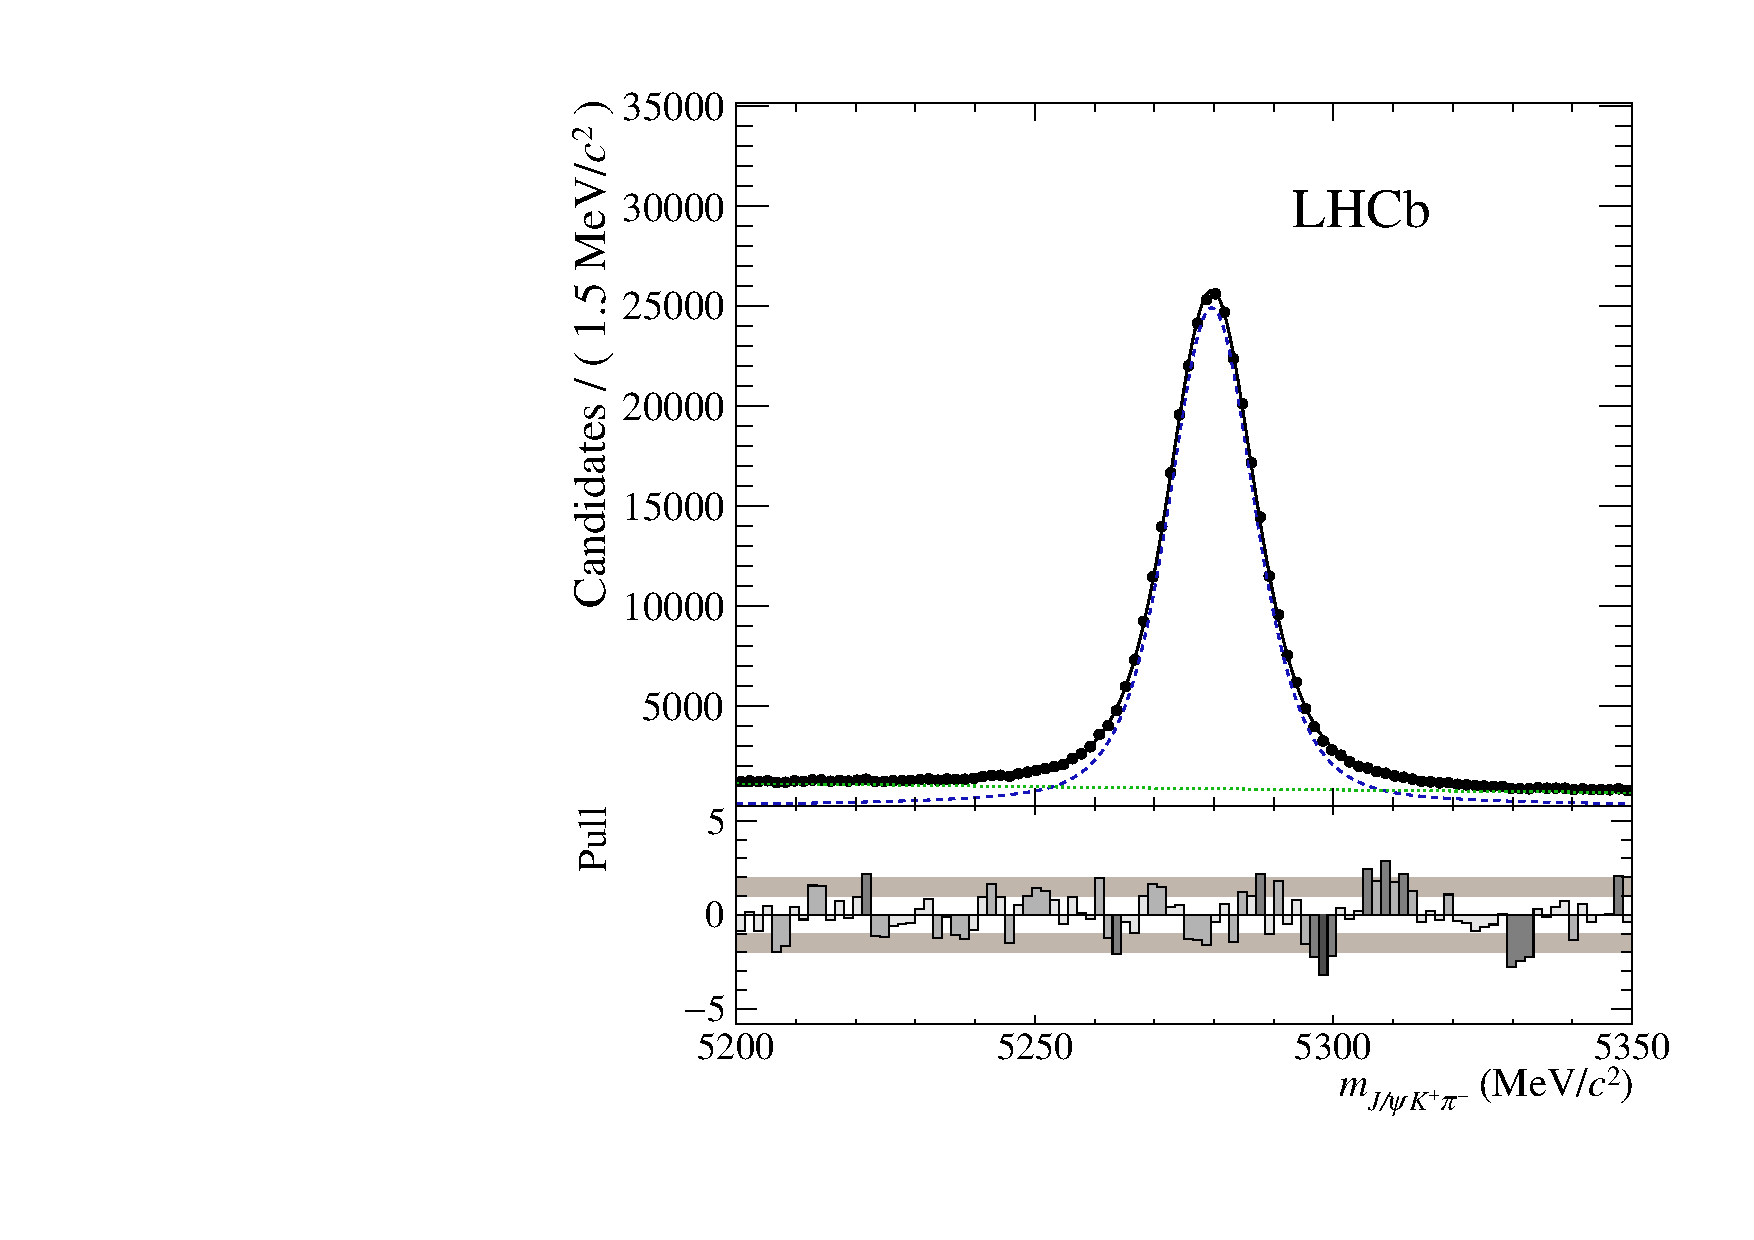
\includegraphics[width=0.5\textwidth]{08FlavourTagging/figs/BmassJpsiKst_pull.pdf}
    \caption{Fit to the invariant mass of the $\Bz\!\to\jpsi\Kstarz$ candidates with a constraint on the known \jpsi mass.
    The data is represented by the black points, the black solid line shows the full PDF, the blue dashed line shows the signal componente and the background component is represented by the dotted yellow line.}
    \label{fig:massFitJpsiKst}
\end{figure}
\begin{table}[tbp]
	\centering
	\caption{Fitted Yields of the $\Bz\!\to\jpsi\Kstarz$ component and the combinatorial background.}
	\begin{tabular}{SS}
		\toprule
		{Parameter} & {Yield} \\
		\midrule
		{$N_{\Bz\!\to\D\pion}^{\pion}$}	& 351507\pm662 \\
		{$N_{\text{bkg}}^{\pion}$}		& 88630\pm419 \\
		\bottomrule
	\end{tabular}
	\label{tab:yieldsJpsiKst}
\end{table}

The last preparation step for the data sample is then to weight certain \emph{sWeighted} distributions of $\Bz\!\to\jpsi\Kstarz$ candidates to match the corresponding distributions of the \BdToDpi candidates.
The observables which are weighted are chosen as they are known to most influence the tagging responses:
These observables are the transverse momentum \pt, the pseudo-rapidity $\eta'$ and the azimuthal angle $\phi$ of the \Bz candidate as well as the number of tracks and the number of \ac{PV}s in the event.
Additionally, an observable containing the composition of the used trigger lines is weighted.
For this observables the categories \num{1}, \num{2} and \num{3} contain candidates which are exclusively triggered TOS by the \verb!Hlt2Topo2BodyBBDTDecision!, \verb!Hlt2Topo3BodyBBDTDecision! or \verb!Hlt2Topo4BodyBBDTDecision! line, respectively.
Category \num{4} contains candidates triggered TOS exclusively by the overlap of the \verb!Hlt2Topo2BodyBBDTDecision! and \verb!Hlt2Topo3BodyBBDTDecision! lines, candidates triggered exculsively TOS by the overlap of the \verb!Hlt2Topo2BodyBBDTDecision! and \verb!Hlt2Topo4BodyBBDTDecision! lines are classified in category \num{5} and candidates triggered exclusively TOS by the overlap of the \verb!Hlt2Topo3BodyBBDTDecision! and \verb!Hlt2Topo4BodyBBDTDecision! lines are in category \num{6}.
The last category (\num{7}) contains candidates which are triggered by all three Hlt2 lines.

Instead of weighting the six-dimensional parameter space using a six-dimensional histogram a BDT based approach is chosen.
In this approach, the parameter space is split in several large regions, which are separated using binary decision trees.
These trees maximise a symmetrised $\chi^2$
\begin{equation}
\chi^2=\sum_{i}\frac{\left(N_{i,\text{source}}-N_{i,\text{target}}\right)^2}{N_{i,\text{source}}+N_{i,\text{target}}}
\end{equation}
where $N_{i,\text{source}}$ are the number of candidates in the $i$th bin of the distribution which should be weighted and $N_{i,\text{target}}$ are the number of candidates in the $i$th bin of the target distribution.
For all leaves of a decision tree a prediction $p$ is calculated following
\begin{equation}
p=\log\frac{N_{i,\text{target}}}{N_{i,\text{source}}}\,,
\end{equation}
what is used to calculate the weights as
\begin{equation}
w=\begin{cases} w, &\, \text{if event from target distribution}\\ we^{p}, &\, \text{if event from source distribution\,\,.} \end{cases}
\end{equation}
These steps are then repeated for each decision tree.
In this case the BDT is built out of \num{40} trees with a maximum depth of three.
Each leave has to contain a minimum number of \num{200} candidates and the boosting method is Gradient boosting~\cite{Friedman00greedyfunction}.
The distributions of the original and weighted $\Bz\!\to\jpsi\Kstarz$ and \BdToDpi candidates is shown in \cref{fig:reweightingSS}.
\begin{figure}[tbp]
    \centering
    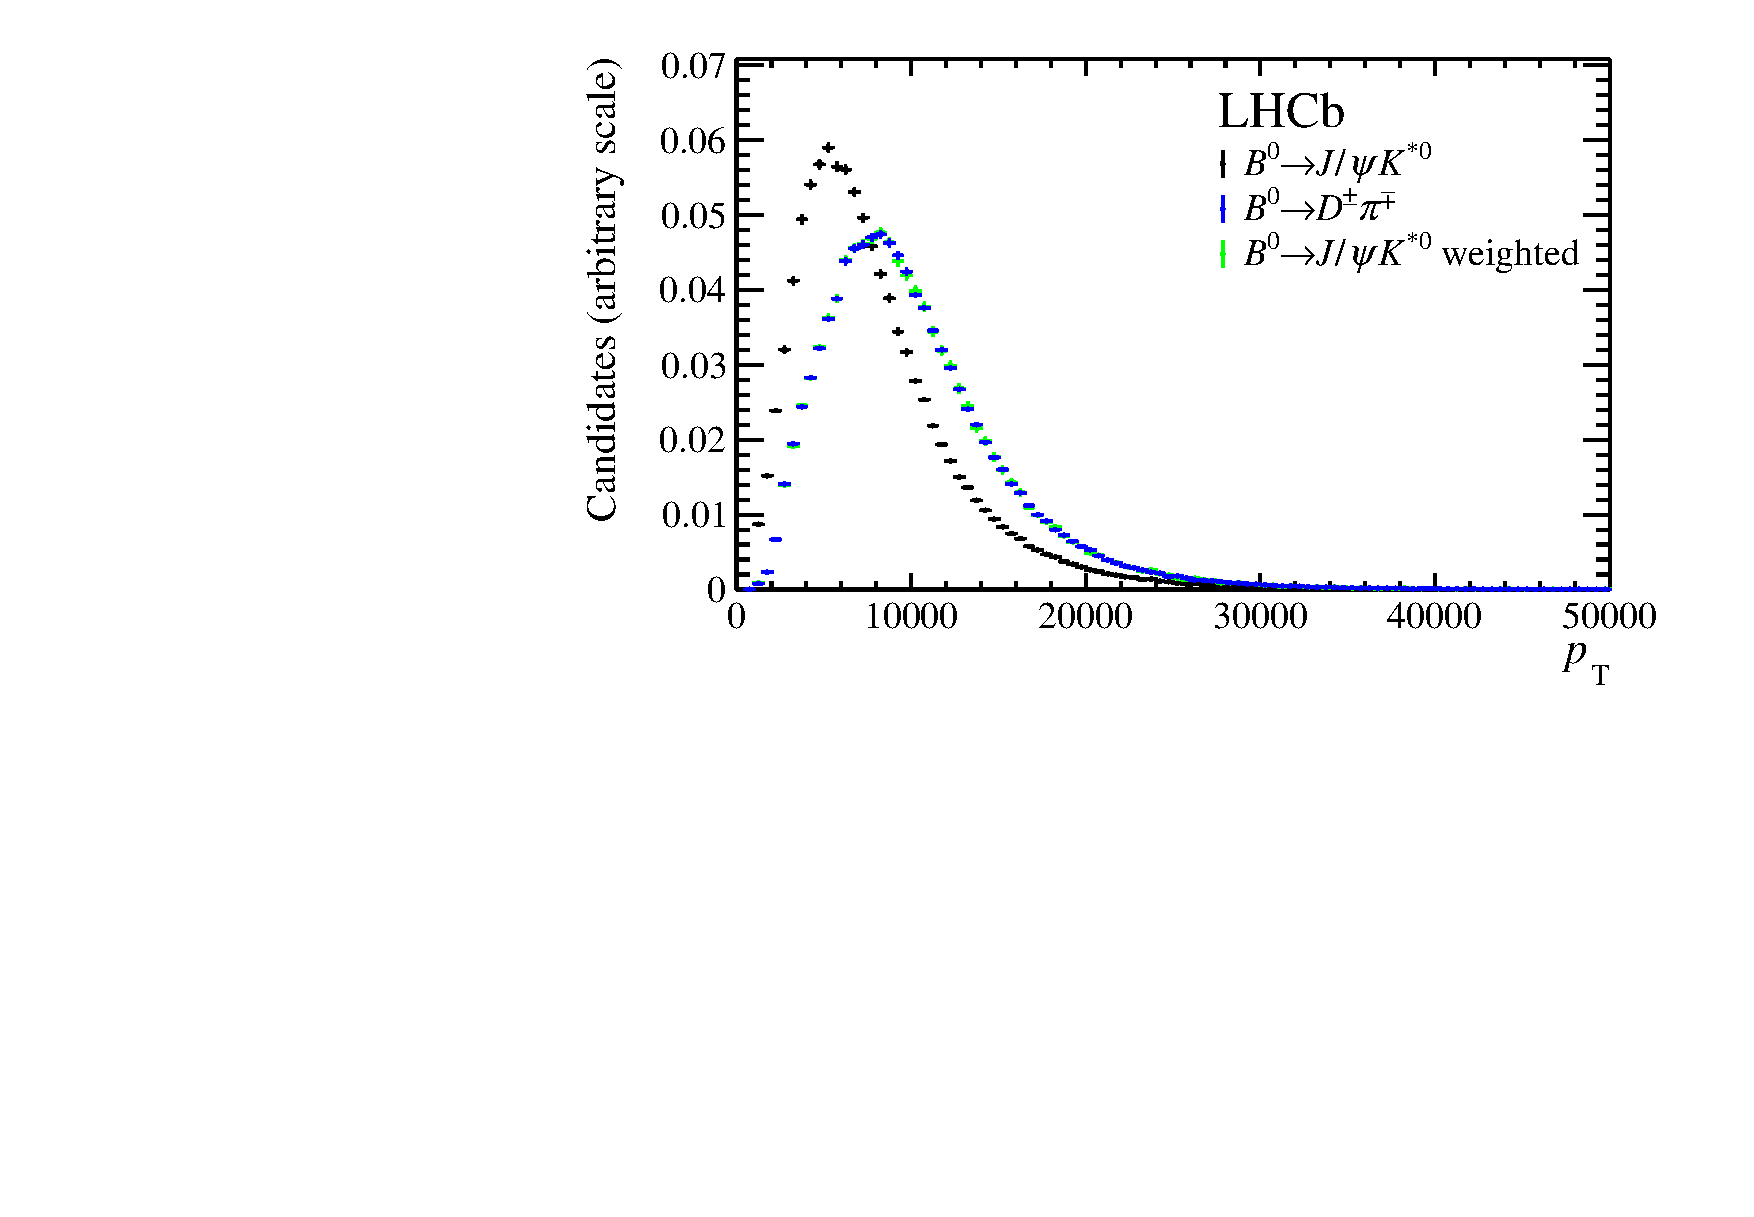
\includegraphics[width=0.48\textwidth]{08FlavourTagging/figs/pT_weighted.pdf}
    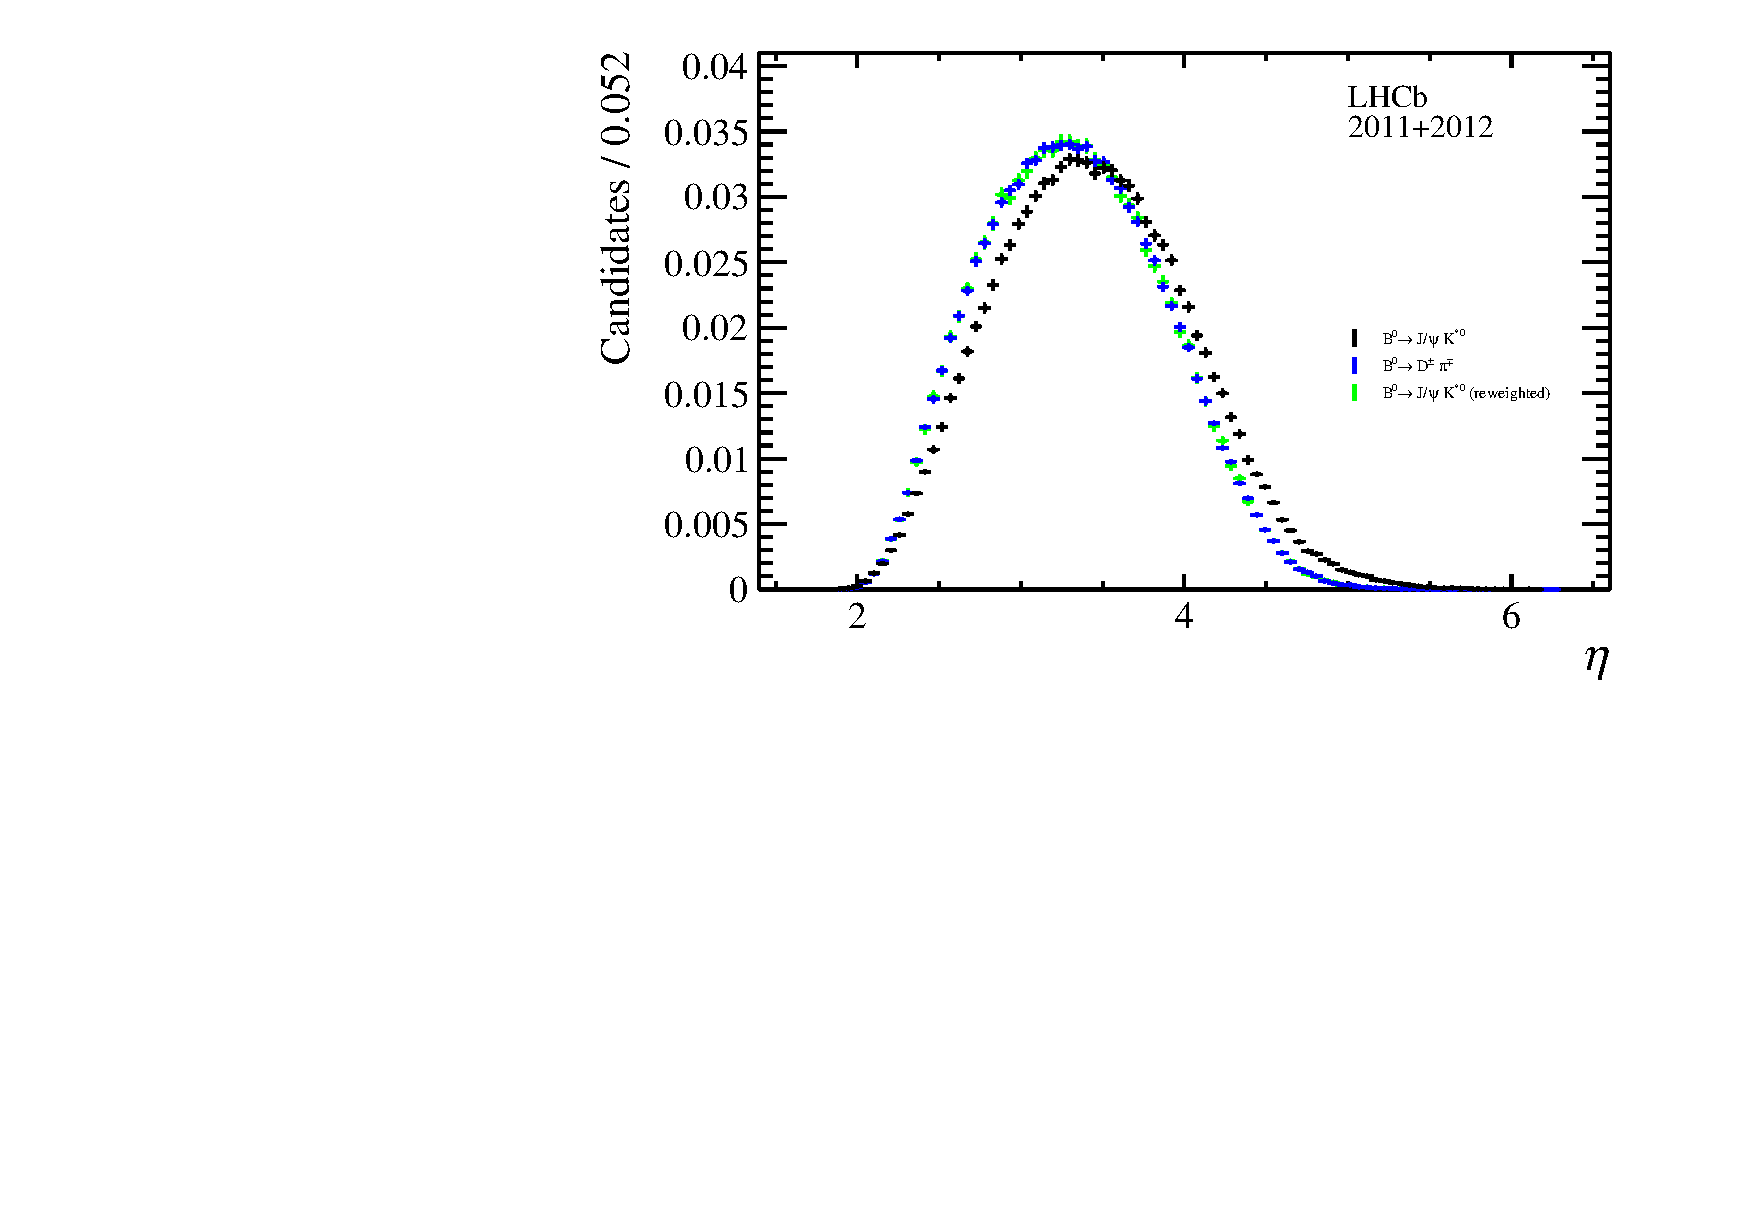
\includegraphics[width=0.48\textwidth]{08FlavourTagging/figs/eta_weighted.pdf}\\
    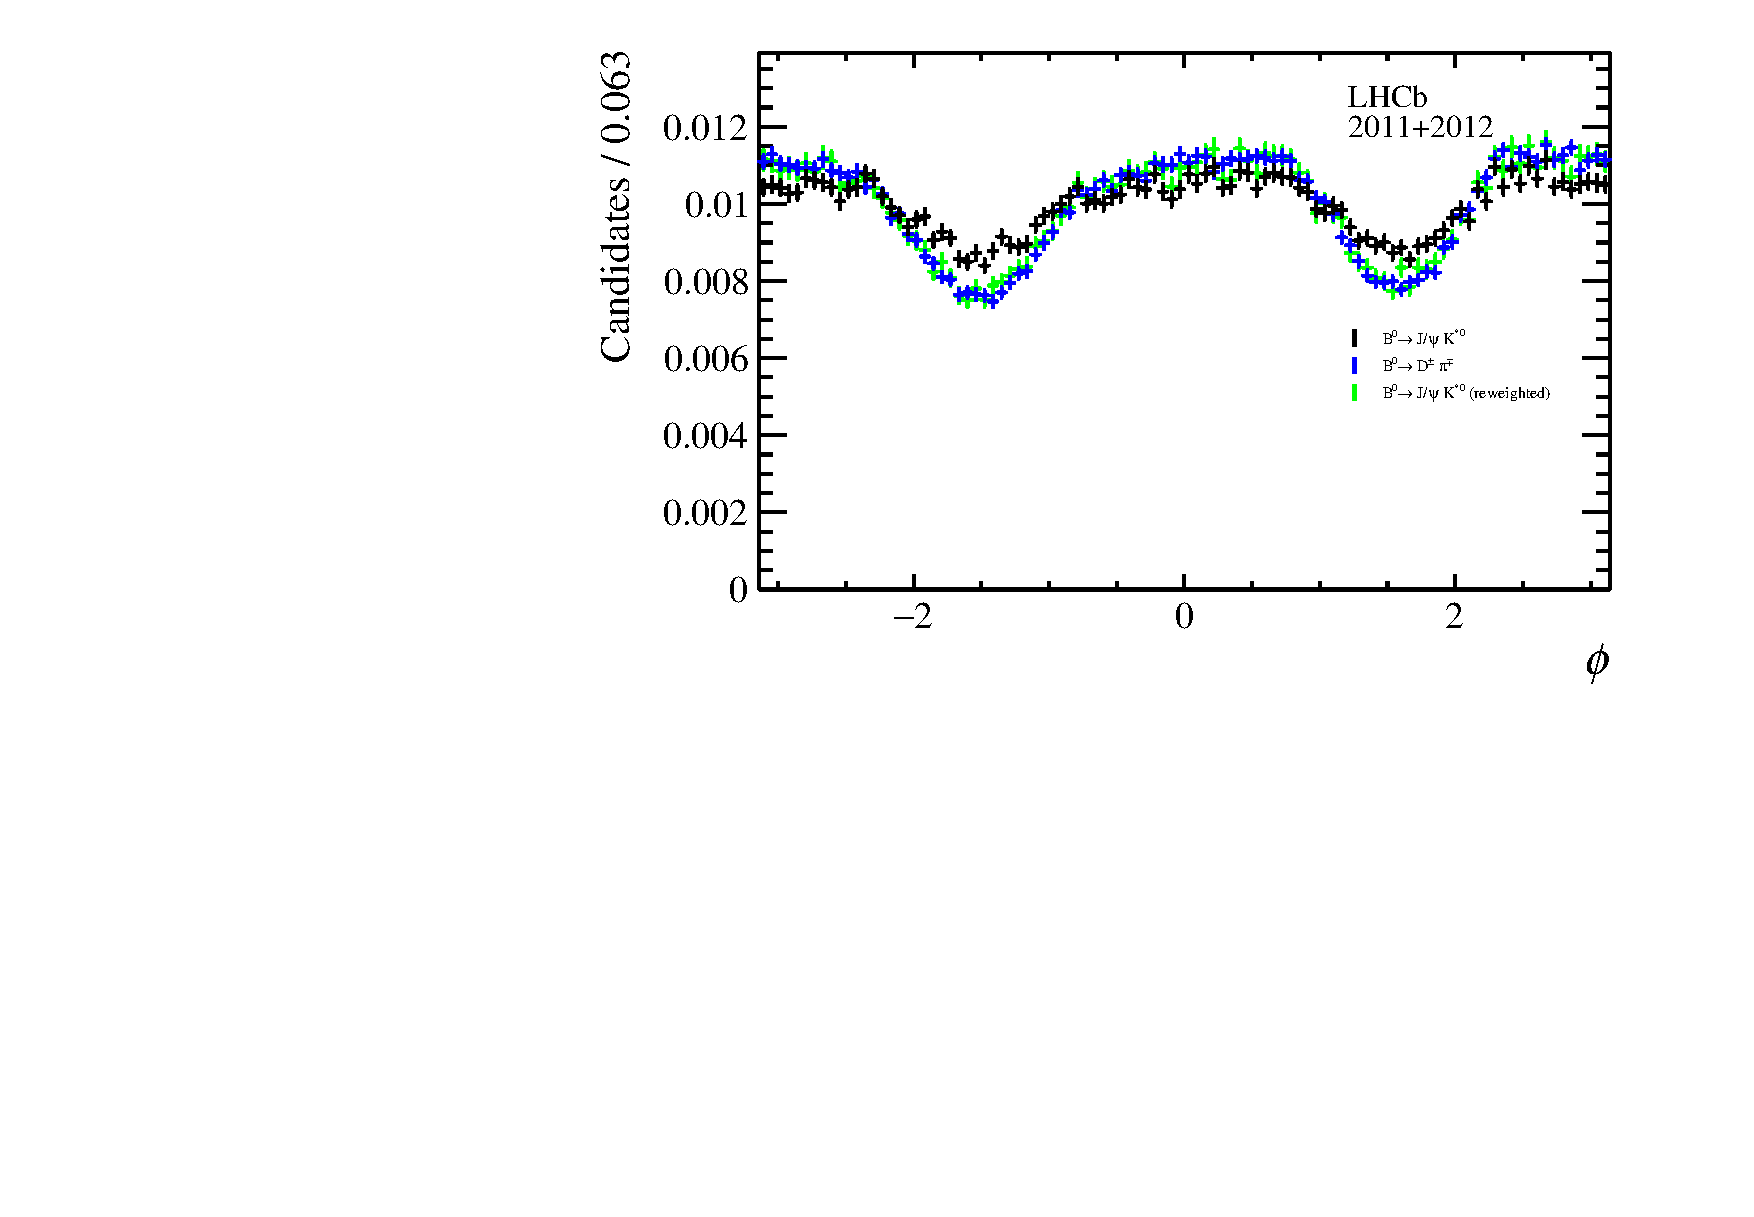
\includegraphics[width=0.48\textwidth]{08FlavourTagging/figs/phi_weighted.pdf}
    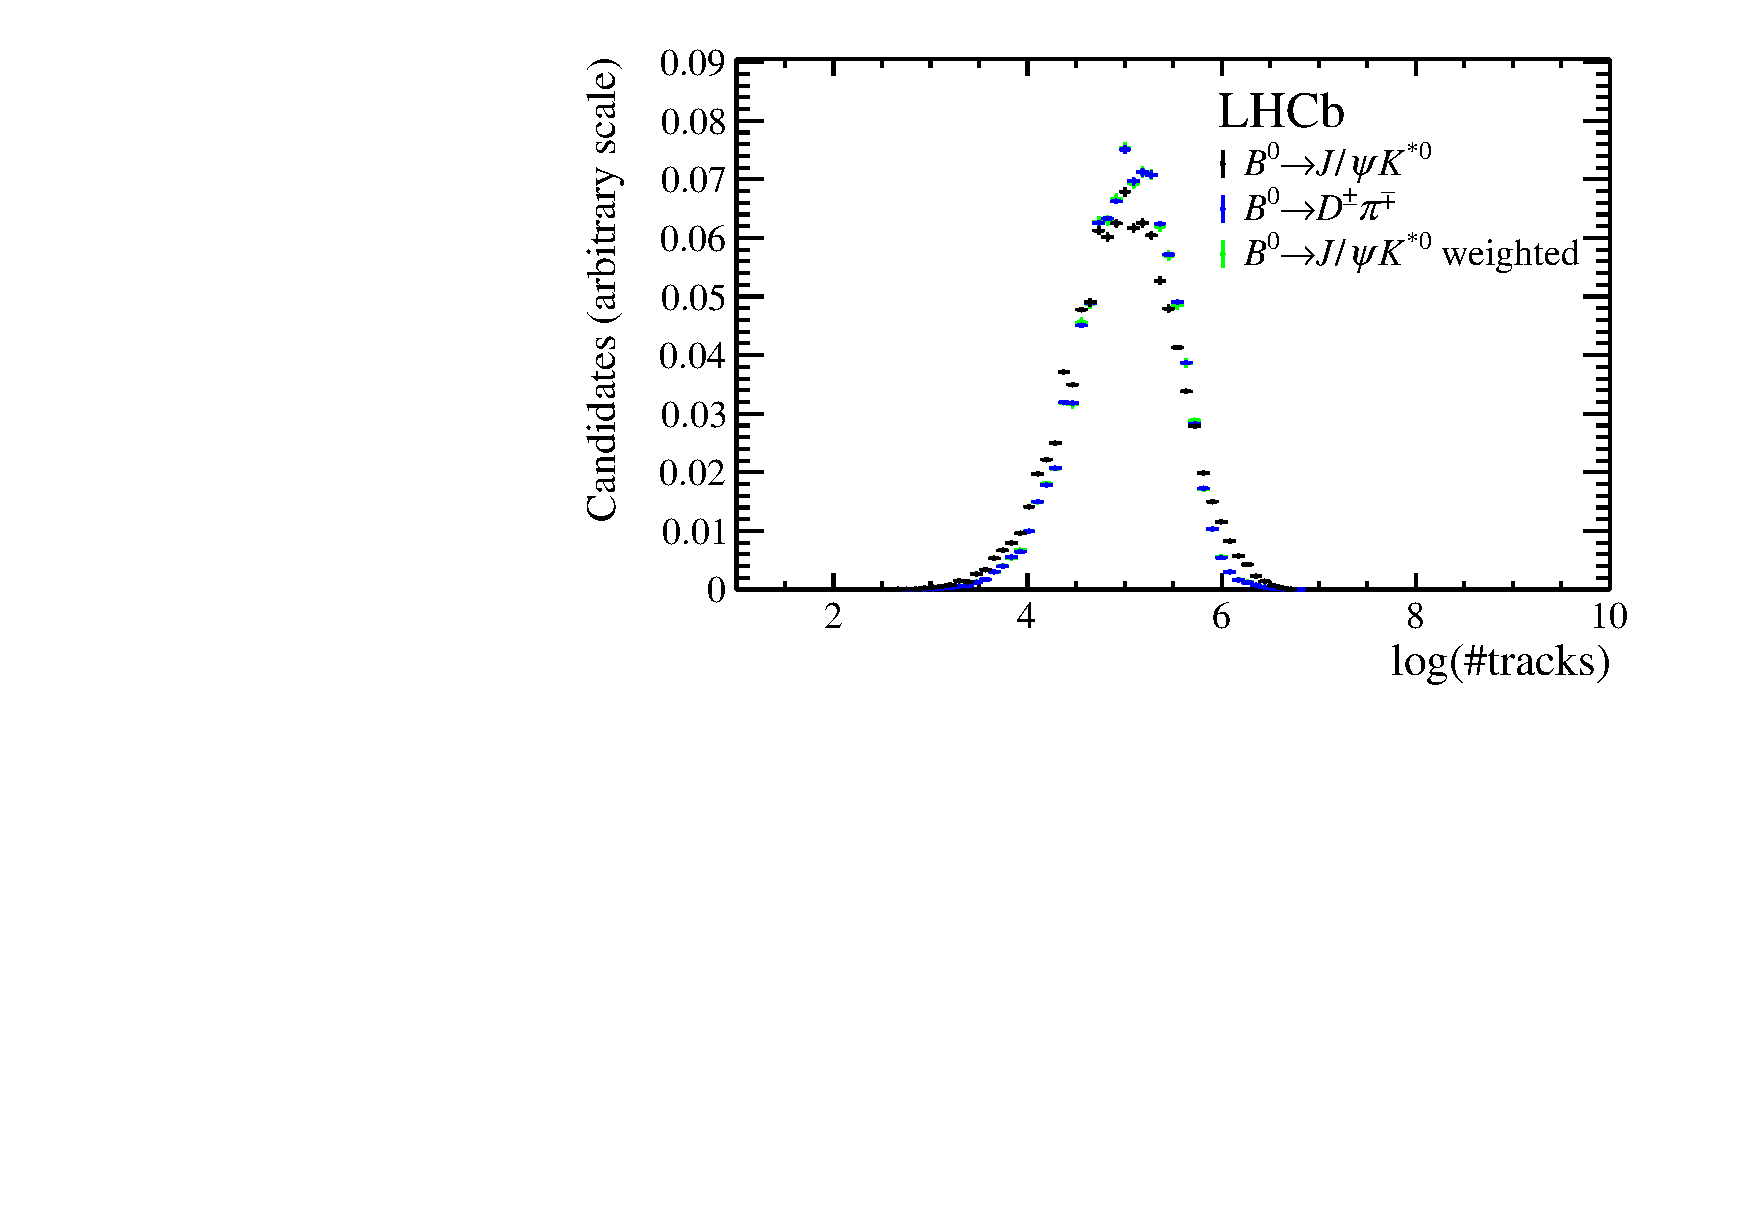
\includegraphics[width=0.48\textwidth]{08FlavourTagging/figs/nTracks_weighted.pdf}\\
    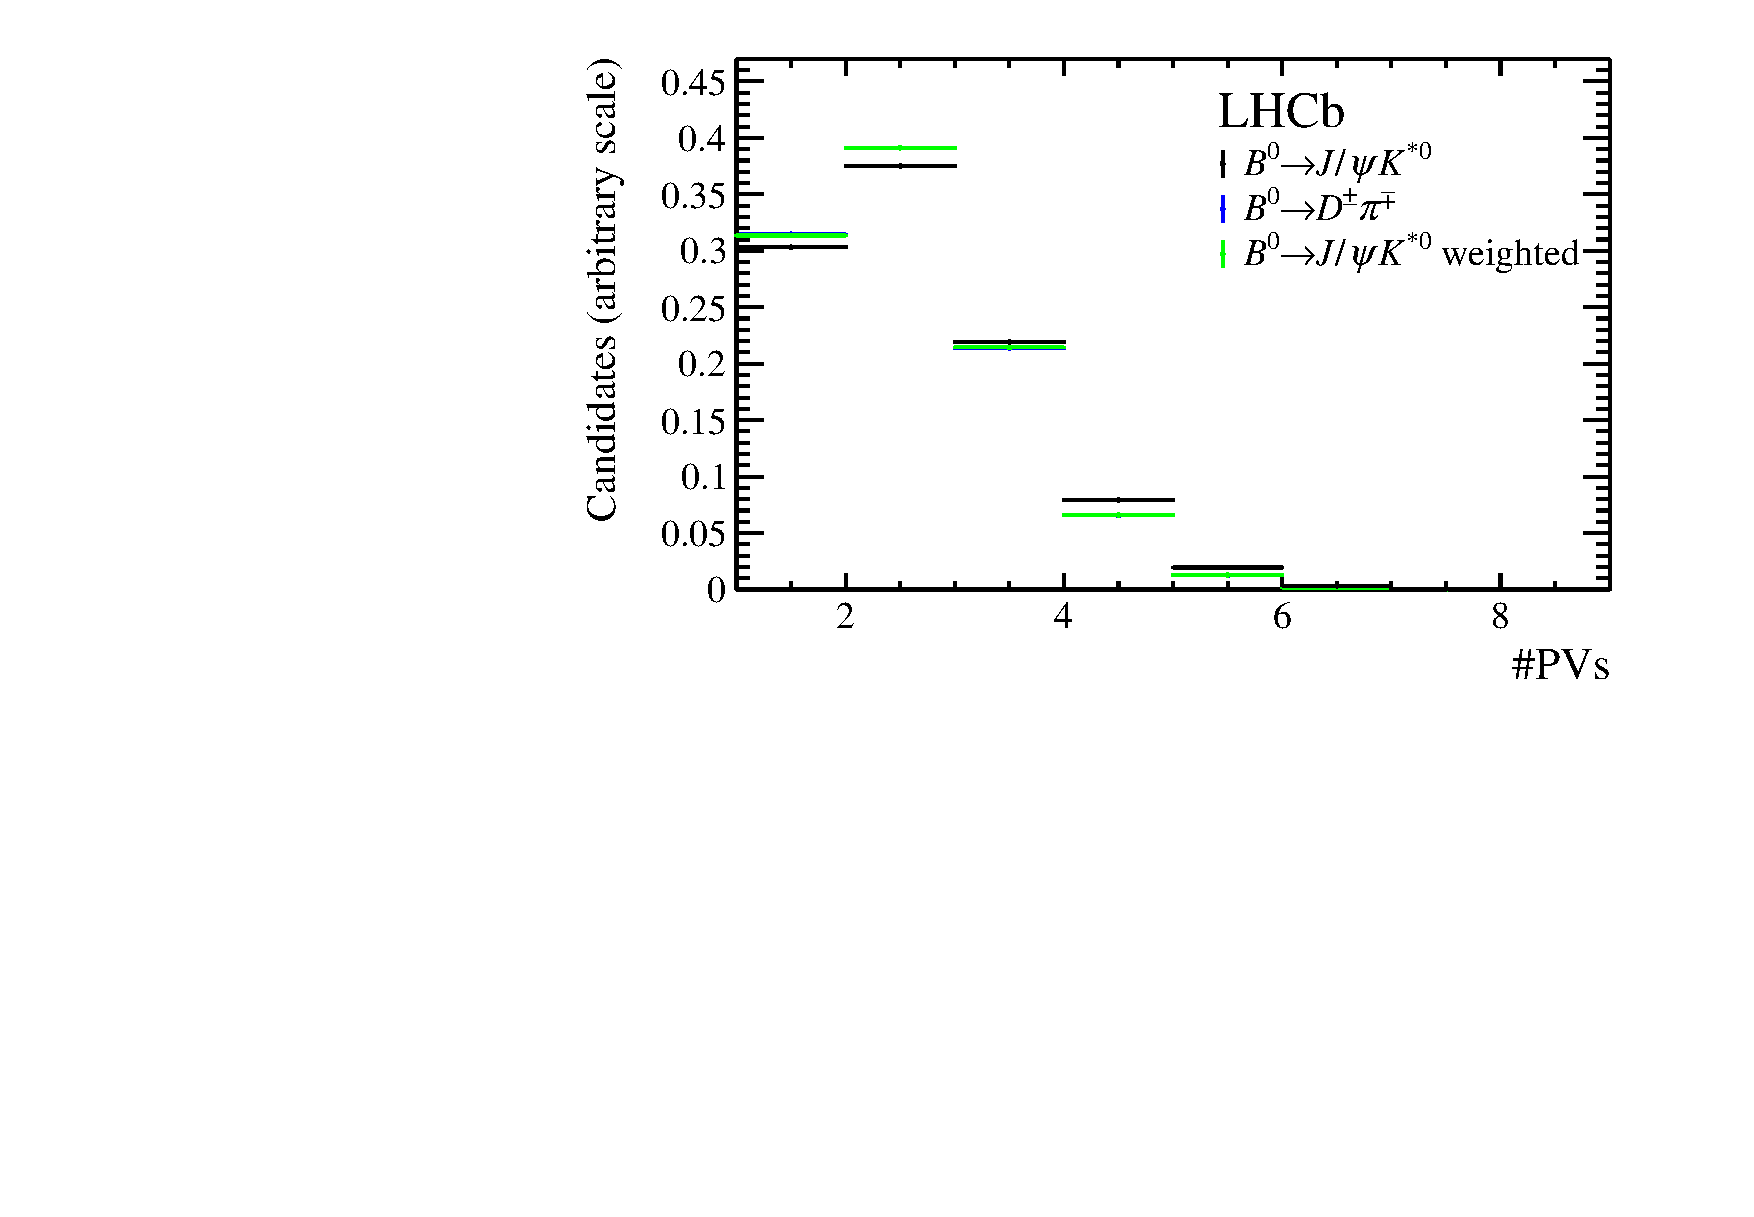
\includegraphics[width=0.48\textwidth]{08FlavourTagging/figs/nPV_weighted.pdf}
    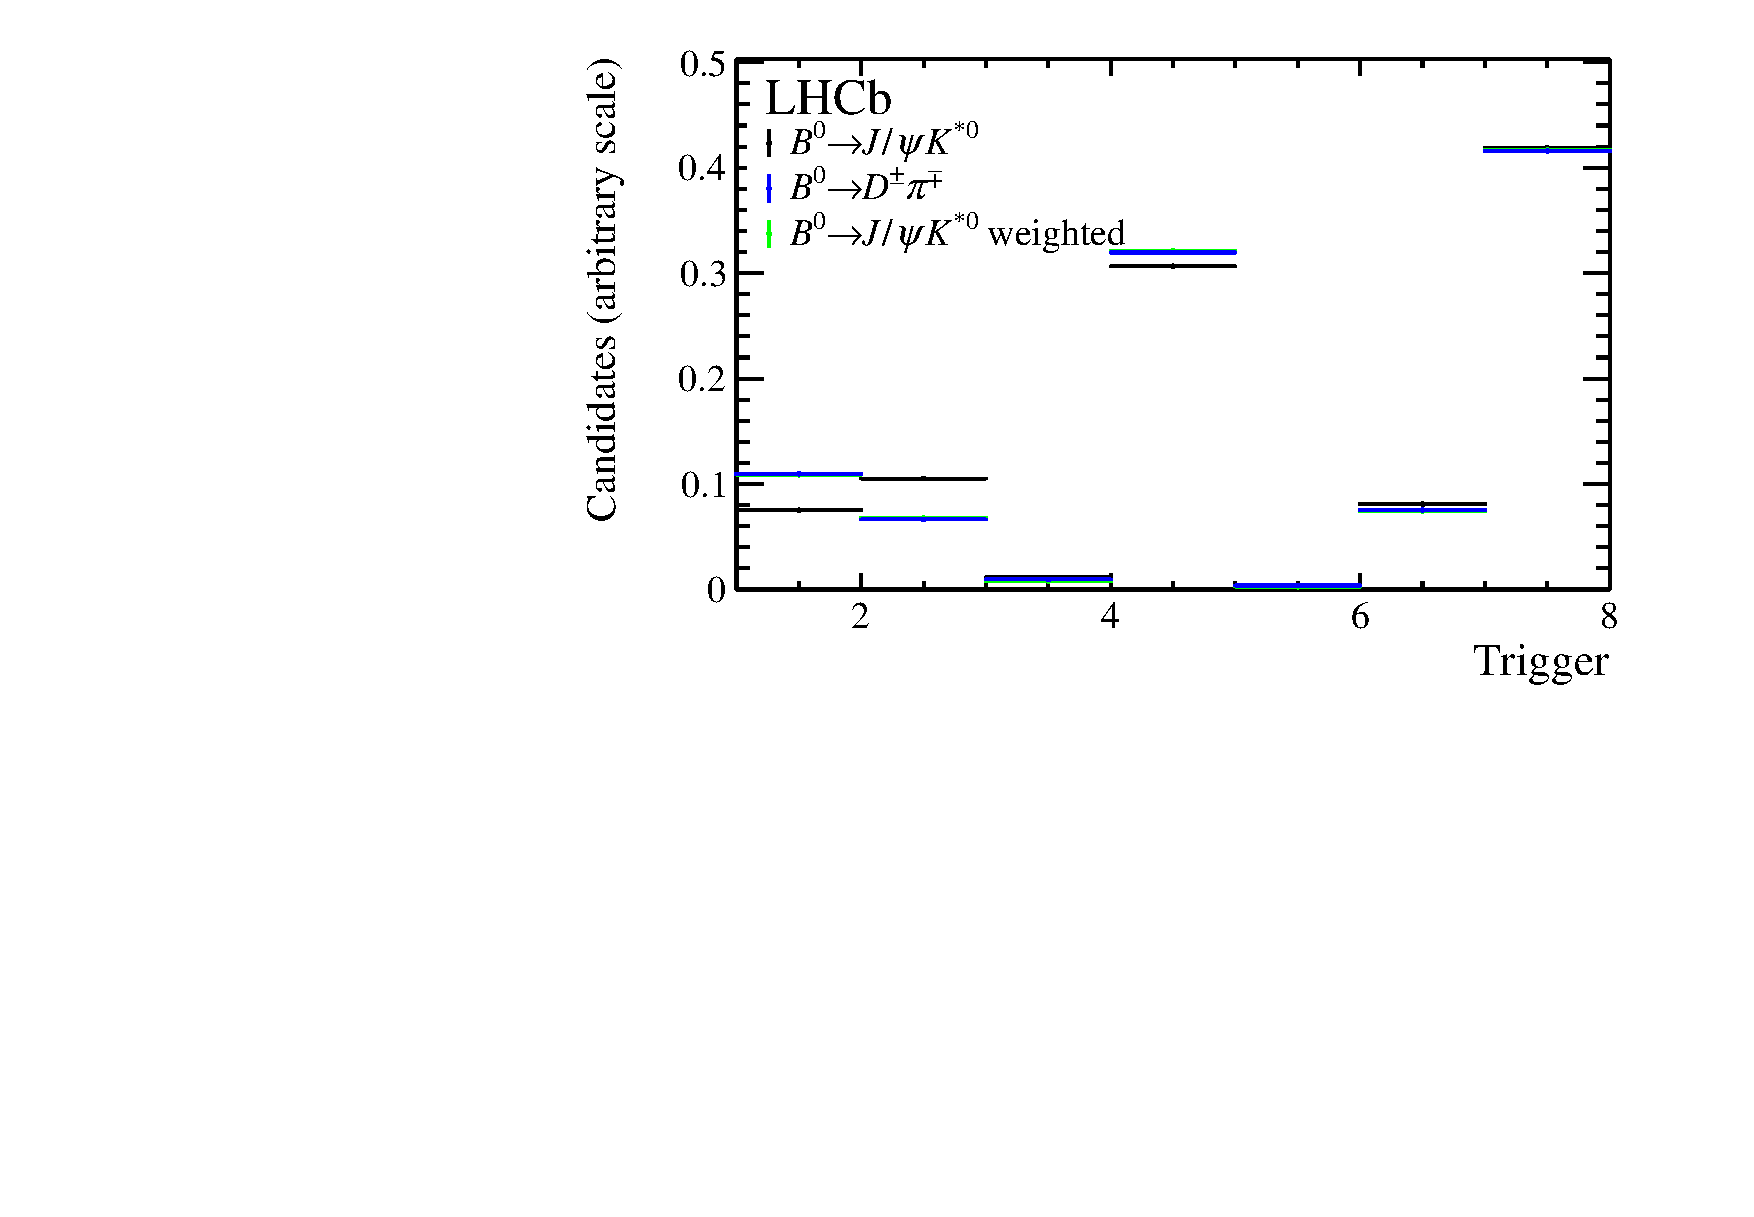
\includegraphics[width=0.48\textwidth]{08FlavourTagging/figs/Trigger_weighted.pdf}
    \caption{Left, top to bottom: Normalised \emph{sWeighted} distributions of the transverse momentum, azimuthal angle and number of tracks per event.
    Right, top to bottom: Normalised \emph{sWeighted} distributions of the pseudo-rapidity, logarithm of number of tracks per event and distribution of trigger decisions.}
    \label{fig:reweightingSS}
\end{figure}

\subsection{Retraining of the SS pion tagger}
\label{sec:retrainSSpion}

First the tagging particles have to fulfill a set of selection cuts, which are partly applied only to the tagging track and partly to the system of the tagging track and the \B candidate. These cuts have two aims:
First separating pions form other charged tracks in the event and second selecting particles which are in the same region of phase space as the \B candidate.
\begin{table}[tbp]
	\centering
	\caption{Selection cuts for the SS pion algorithm.
	The first set of cuts is applied only top the tagging-particle track, while the second set is applied to the \enquote{tagging-particle track+\B} system.}
	\begin{tabular}{cc}
		\toprule
		Variable & Cut \\
		\midrule
		transverse momentum \pt 											& $>\SI[per-mode=symbol]{0.4}{\GeVc}$ \\
		$\nicefrac{\text{IP}}{\sigma_{\text{IP}}}$							& $<4$ \\
		track ghost probability $g_{\text{prob}}$ 							& $<0.5$ \\
		\dllppi 															& $<5$ \\
		\dllkpi 															& $<5$ \\
		track $\nicefrac{\chi^2}{\text{ndof}}$ 								& $<5$ \\
		$\nicefrac{\text{IP}_{\text{PU}}}{\sigma_{\text{IP}_{\text{PU}}}}$ 	& $>3$ \\
		\midrule
		transverse momentum \pt 					& $>\SI{3}{\GeVc}$ \\
		$\Delta Q=m_{\B+\pion}-m_{\B}-m_{\pion}$ 	& $<\SI{1.2}{\GeVcc}$ \\
		$\Delta\eta'$								& $<1.2$ \\
		$\Delta\phi$								& $<1.1$ \\
		vertex $\chi^2$ 							& $<100$ \\
		\bottomrule
	\end{tabular}
	\label{tab:SSPionselectionCuts}
\end{table}
For each tagging-particle candidate passing the requirements shown in \cref{tab:SSPionselectionCuts}, the \B-meson gets a preliminary tag decision assigned, corresponding to the charge of the tagging particle (\mbox{$\pip\rightarrow d=+1$}, \mbox{$\pim\rightarrow d=-1$}).
The quantities $\Delta\eta'$ and $\Delta\phi$ describe the difference of pseudo-rapidity and azimuthal angle between the signal and tagging-particle track.
To further assure that the tagging-particle is also produced at the \ac{PV} with which the \B candidate has the smallest $\text{IP}\chi^2$, the impact parameter significance with the next \enquote{best} PV in the event (denoted as pile-up vertex) is used.
The corresponding quantities are $\nicefrac{\text{IP}}{\sigma_{\text{IP}}}$ and $\nicefrac{\text{IP}_{\text{PU}}}{\sigma_{\text{IP}_{\text{PU}}}}$, respectively.

Subsequent a BDT is trained to determine the mistag and to select the best tagging-particle candidate in events with more than one tagging-particle candidate passing  the selection in \cref{tab:SSPionselectionCuts}.
In the training, all candidates with the correct correlation between the preliminary tag and the \B-flavour are considered as signal, all with the wrong correlation are considered background.
A correct or wrong correlation for the SS pion algorithm means
\begin{align*}
	\text{Correct tag: }& \Bz\pip \text{ or } \Bzb\pim\,,\\
	\text{Wrong tag: }& \Bz\pim \text{ or } \Bzb\pip
\end{align*}
where only \B candidates with a decay time smaller than \SI{2.2}{\pico\second} are used in the BDT training to reduce the number of oscillated \B candidates.
The BDT further consists of \num{3000} trees with a maximum depth of two.
Each tree uses up to five of the input variables scanned at 30 points to find the optimal cut point.
As boost algorithm AdaBoost~\cite{AdaBoost} is chosen with a boost factor of $\beta=0.005$.
A list of the input variables is given in \cref{tab:BDTInputSSPion}.
\begin{table}[tbp]
	\centering
	\caption{List of input variables used in the training of the BDT for the SS pion tagger.
	The quantity $\mathrm{ProbNNK}$ is the probability for a particle to be a kaon, calculated by an artificial neural network using information from the \lhcb PID system.
	The momentum of a particle is denoted as $p$.}
	\begin{tabular}{cc}
		\toprule
		\multirow{6}{*}{tagging-particle inputs} 	& $\log\left(\pt\right)$ \\
													& $\log\left(p\right)$ \\
													& $\log\left(\text{IP}/\sigma_\text{IP}\right)$\\
													& $\log\left(g_\text{prob}\right)$\\
													& $\log\left(\text{track} \nicefrac{\chi^2}{\text{ndof}}\right)$ \\
													& $\log\left(\text{ProbNNK}\right)$\\
		\midrule
		\multirow{5}{*}{tagging-particle + $\Bz$ inputs}	& $\Delta Q$\\
															& $\Delta R$\\
															& $\log\left(\Delta\eta'\right)$\\
															& $\log\left(\Delta\phi\right)$\\
															& $\log\left(\pt\right)$\\
		\midrule
		\multirow{1}{*}{event properties}	& PVndof\\
		\bottomrule
	\end{tabular}
	\label{tab:BDTInputSSPion}
\end{table}
\begin{figure}[tbp]
	\begin{center}
		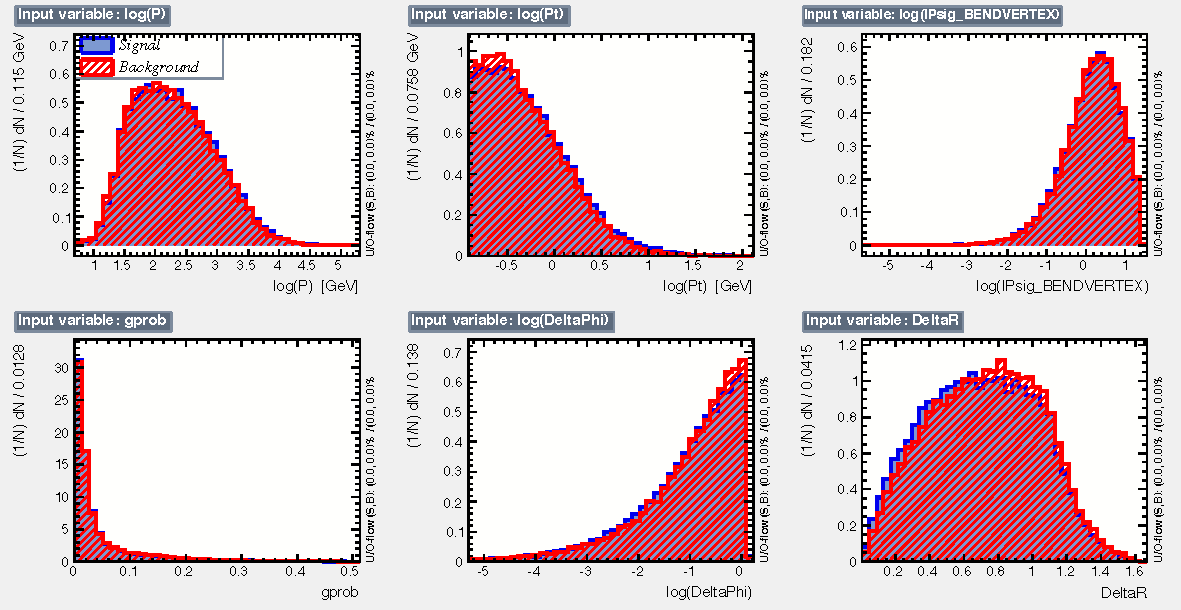
\includegraphics[width=0.8\textwidth]{08FlavourTagging/figs/SSpionBDT_input1.pdf}\\
		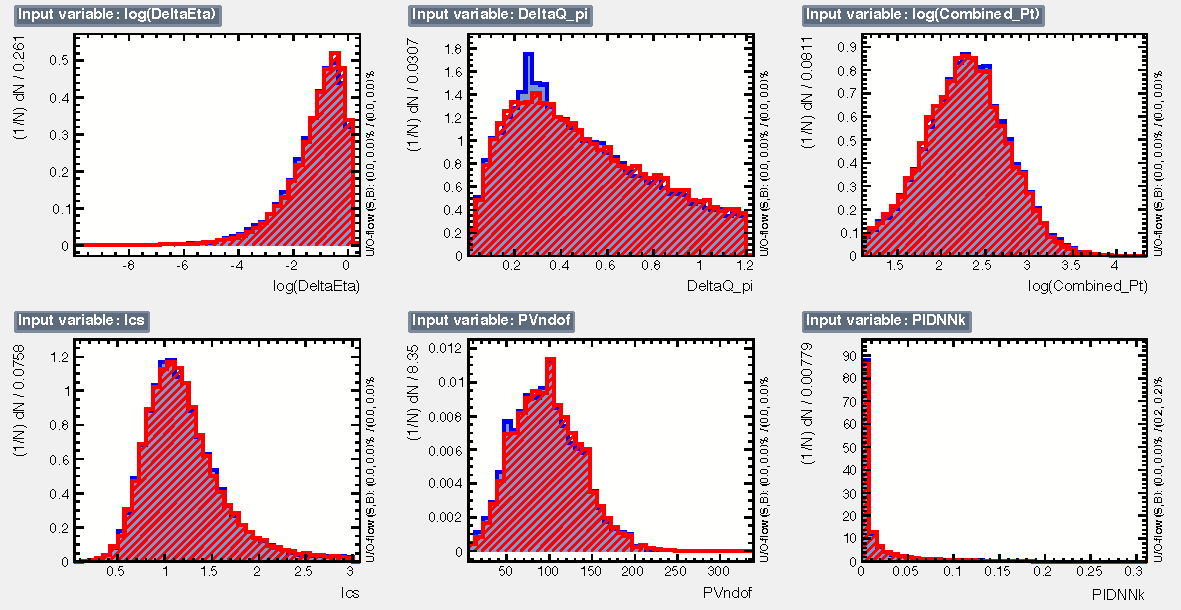
\includegraphics[width=0.8\textwidth]{08FlavourTagging/figs/SSpionBDT_input2.pdf}
	\end{center}
	\caption{Distributions of the input variables used in the BDT training.
	The blue curve represents the right charge correlation while the red curve corresponds to the wrong ones.}
	\label{fig:BDTInputSSPion}
\end{figure}
Most of these variables were already used in the selection, PVndof is the number of degrees of freedom in the fit to determine the position of the \ac{PV} and $\Delta R=\sqrt{\Delta\phi^2+\Delta\eta'^2}$.
Moreover a logarithmic transformation is applied to some of the input variables to improve the performance of the BDT.
As one can see in \cref{fig:BDTInputSSPion} the distributions of the signal and background samples are quite similar.
This small, but significant difference is propagated to the distribution of the BDT response as shown in \cref{fig:BDTovertrainSSPion}.
\begin{figure}[tbp]
	\begin{center}
		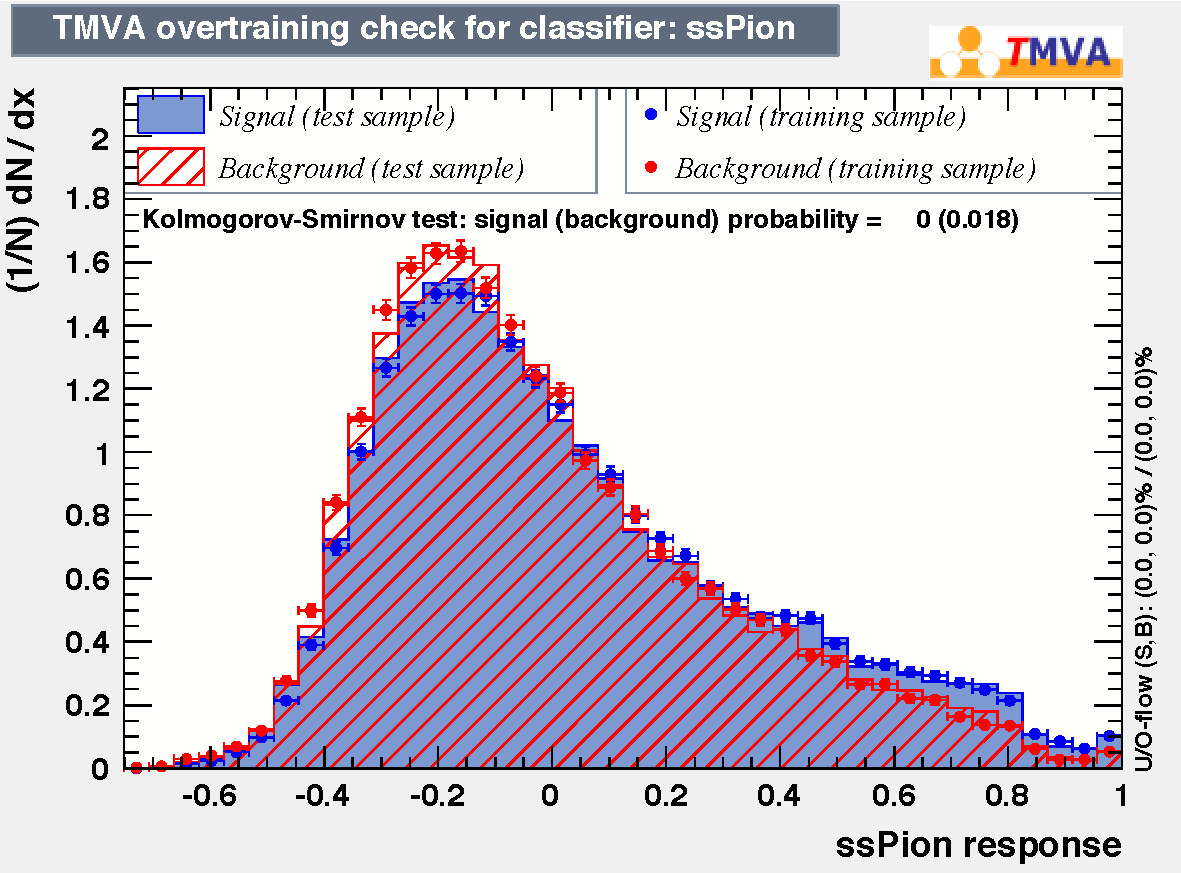
\includegraphics[width=0.6\textwidth]{08FlavourTagging/figs/SSPionBDT_overtrain.pdf}
	\end{center}
	\caption{Output of the SS pion BDT ($\alpha^{\text{SS}\pion}_\text{BDT}$).
	The blue distribution represents the right charge correlated tracks while the red distribution corresponds to the wrong charge correlated tracks.}
	\label{fig:BDTovertrainSSPion}
\end{figure}
For events with more than one tagging particle, the best one is identified as the particle with the largest BDT output.

Subsequently, due to the flavour oscillations, a time-dependent analysis is necessary to transform the BDT response into a mistag.
For this, an unbinded maximum-likelhihood fit to the decay-time $t$, the tag decisions $d$ and the mixing state $\xi$ is performed.
The mixing state takes values of $+1$ when the \B-meson flavour at decay is the same as the tag decision and $-1$ otherwise.
As the fit is performed to the \emph{sWeighted} decay-time distribution the describing PDF consists only of a signal-component
\begin{equation}
\mathcal{M}(t;d,\xi)=\mathcal{N}a(t)e^{-t'/\tau}\left(\left(1-d\Delta\omega\right)+\xi\left(1-2\omega\right)\cos\!\left(\dm t'\right)\right)\otimes\mathcal{R}(t-t')\label{eq:mixPDF}
\end{equation}
where $\mathcal{N}$ is a normalisation factor and $\omega$ and $\Delta\omega$ are the mistag and mistag difference for initial \Bz- and \Bzb-mesons, respectively.
$\mathcal{R}(t-t')$ describes an average decay time resolution of \SI{50}{\femto\second}.
The lifetime is constrained by means of a Gaussian function to be $\tau=\num{1.518\pm0.004}$ what allows to float the parameters of the cubic-splines describing the decay-time acceptance $a(t)$.
These cubic-splines have five knots placed at $[0.2, 0.25, 2.0, 13.8, 14.5]\,$\si{\pico\second} (more details in \cref{sec:acceptance}).
At first the fit is performed in bins of the BDT response to determine pairs of the average BDT response and mistag.
These pairs are then used to determine the functional form of the transformation and a $3^{\text{rd}}$ order polynomial of the form
\begin{equation}
\omega\left(\alpha^{\text{SS}\pion}_\text{BDT}\right)=b_0+b_1\times\alpha^{\text{SS}\pion}_\text{BDT}+b_2\times{\alpha^{\text{SS}\pion}_\text{BDT}}^2+b_3\times{\alpha^{\text{SS}\pion}_\text{BDT}}^3\label{eq:tranformfunc}
\end{equation}
is found to describe the relation well.
However, to determine the final transformation parameters, an unbinned fit, where the mistag is parametrised directly in the PDF, is performed.
Figure \eqref{fig:MixingSSPion} shows the projected mixing asymmetry from the decay-time fit, defined as
\begin{equation}
A(t)=\frac{N_{\text{unmix}}(t)-N_{\text{mix}}(t)}{N_{\text{unmix}}(t)+N_{\text{mix}}(t)}\propto\left(1-2\omega\right)\cos\!\left(\dm t\right)
\end{equation}
where $N_{\text{unmix}}(t)$ and $N_{\text{mix}}(t)$ are the number of unmixed  and mixed \Bz candidates for a decay time $t$, respectively.
\begin{figure}[tbp]
	\begin{center}
		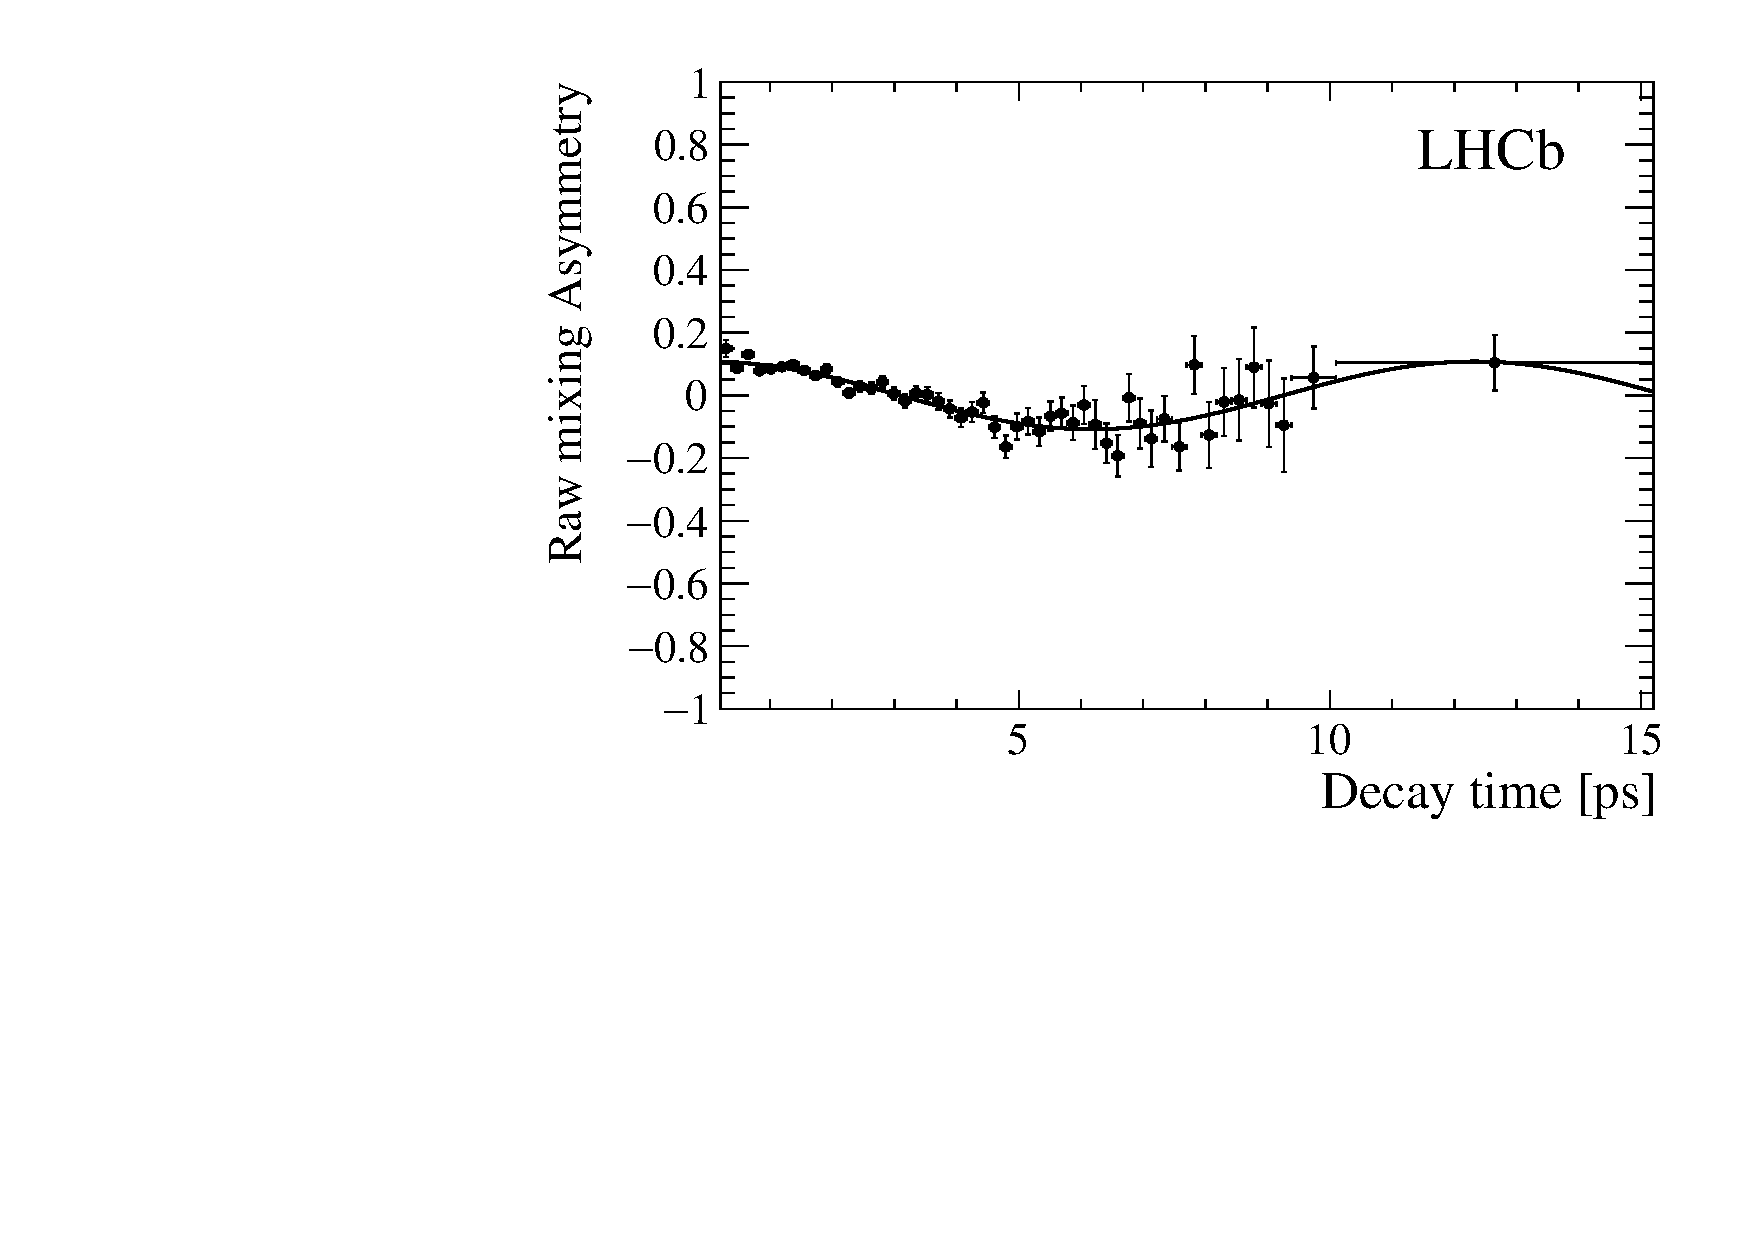
\includegraphics[width=0.6\textwidth]{08FlavourTagging/figs/Asymmetry_SSPion.pdf}
	\end{center}
	\caption{Mixing asymmetry for $\Bz\!\to\jpsi\Kstarz$ candidates tagged by the SS pion tagger.
	The curve overlaid is the fit projection of the decay-time fit.}
	\label{fig:MixingSSPion}
\end{figure}
The resulting transformation parameters are given in \cref{tab:transformationSSPion}, while \cref{fig:transformationSSPion} shows the corresponding $3^{\text{rd}}$ order polynomial.
\begin{table}[tbp]
	\centering
	\caption{Final transformation parameters for the BDT responst of the SS pion tagger.}
	\begin{tabular}{cccc}
		\toprule
		$b_0$ & $b_1$ & $b_2$ & $b_3$ \\
		\midrule
		\num{0.469\pm0.003} & \num{-0.066\pm0.012} & \num{-0.022\pm0.048} & \num{-0.026\pm0.056} \\
		\bottomrule
	\end{tabular}
	\label{tab:transformationSSPion}
\end{table}
\begin{figure}[tbp]
	\begin{center}
		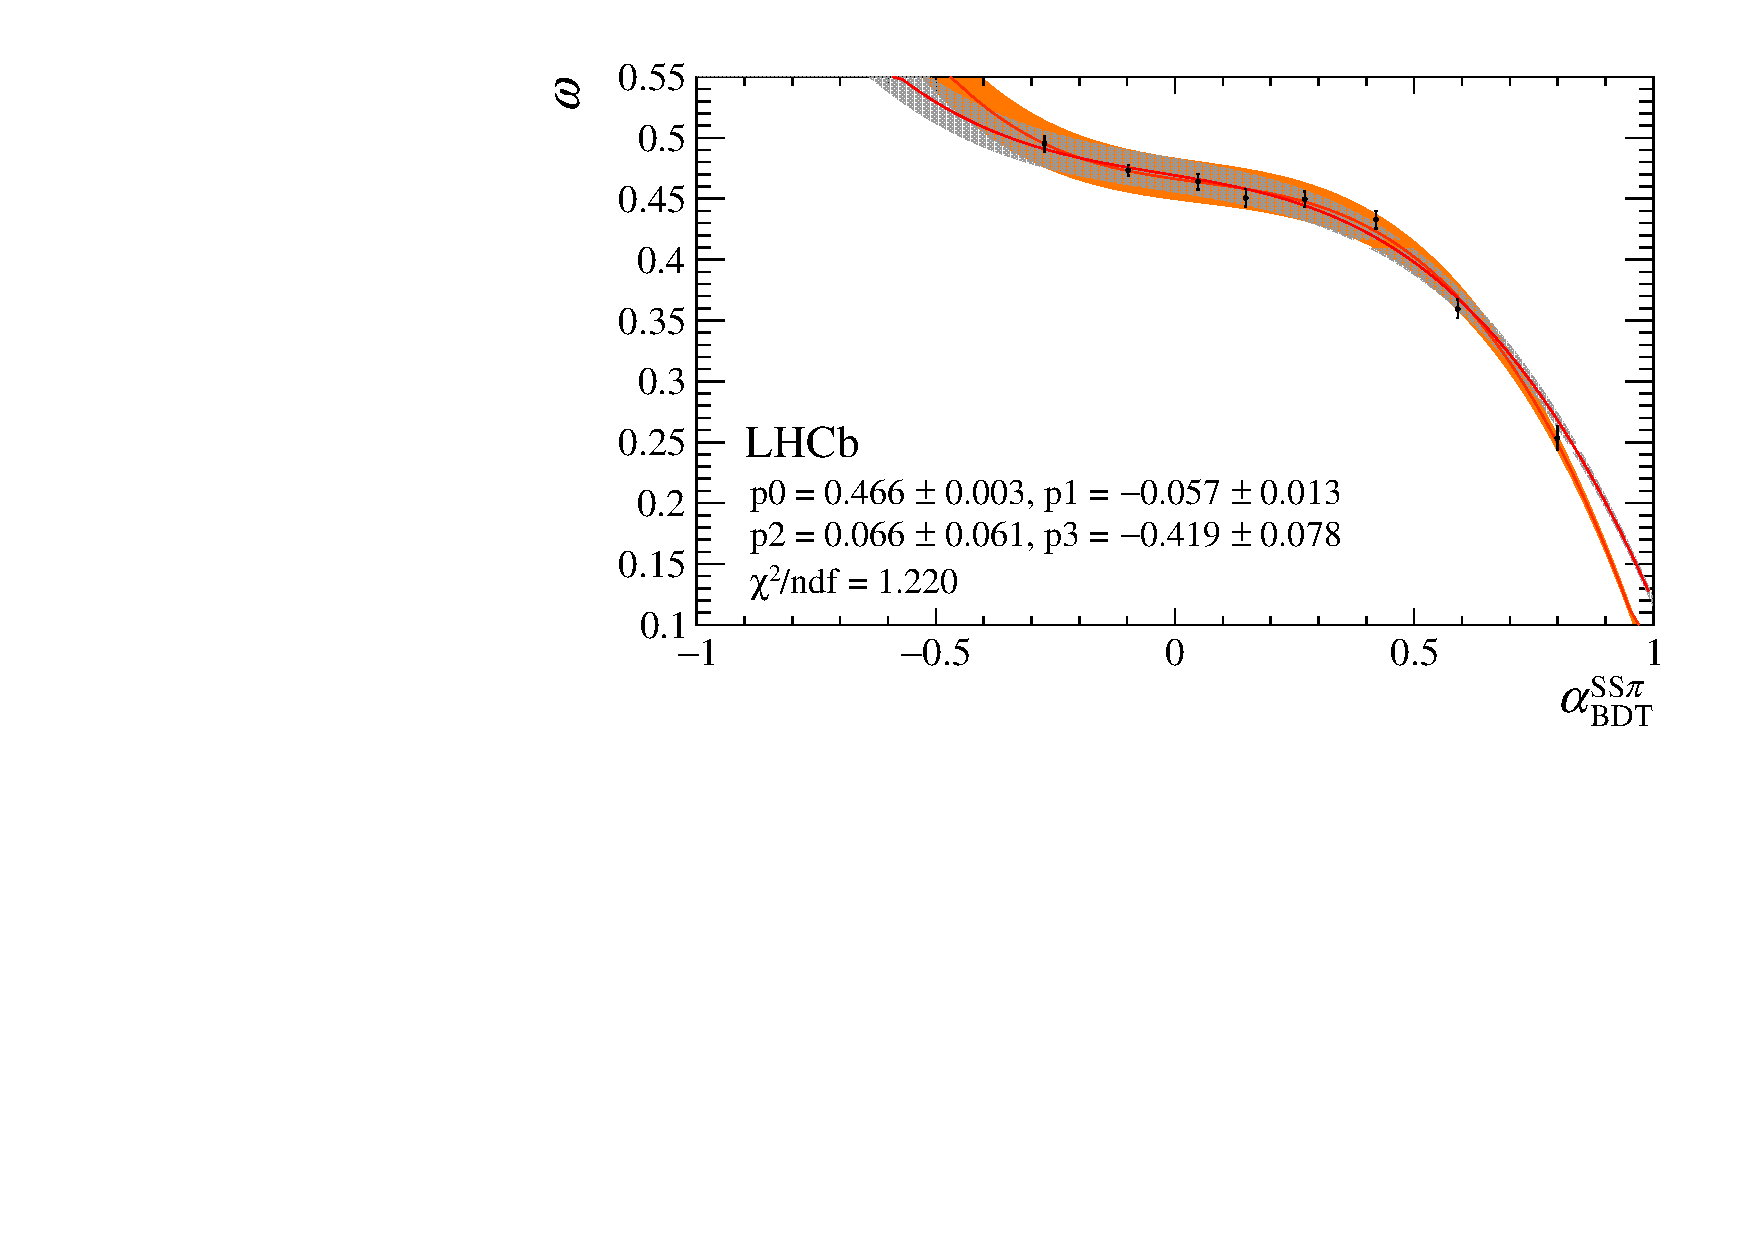
\includegraphics[width=0.6\textwidth]{08FlavourTagging/figs/SSPionBDTTrafo.pdf}
	\end{center}
	\caption{Polynomial curve of $\omega$ versus $\alpha^{\text{SS}\pion}_\text{BDT}$ on the first two thirds of the $\Bz\!\to\jpsi\Kstarz$ data sample.
	The fit from the binned approach is shown in orange, the curved of the nominal unbinned method is shown in grey .
	The parameter values in the plot correspond to the orange curve/binned approach.}
	\label{fig:transformationSSPion}
\end{figure}
Using this transformation for each \Bz candidate the mistag final mistag $\eta$ is calculated.
In case the computed mistag $\eta'$ is larger than \num{0.5}, the tag decision is inverted and the final mistag is calculated as $\eta=1-\eta'$.

\subsection{Retraining of the SS proton tagger}
\label{sec:retrainSSproton}

The procedure for tuning the SS proton tagger BDT and transforming the BDT response is very similar to the one described in \cref{sec:retrainSSpion} for the SS pion tagger.

Besides pions, protons, which have a correlation with the initial flavour of the \B-meson, may also be formed in the hadronisation process.
These tagging-proton candidates must first meet a set of requirements for the proton track itself and the system of the tagging-proton candidate and the \B-meson.
These cuts are listed in \cref{tab:selectionSSProton}.
The correlation between charge of the proton and the \B-meson flavour for the SS proton tagger is as follows:
\begin{align*}
	\text{Correct tag: }& \Bz\antiproton \text{ or } \Bzb\proton\,,\\
	\text{Wrong tag: }& \Bz\proton \text{ or } \Bzb\antiproton\,.
\end{align*}
Based on the charge of the selected particles, consequently a preliminary tag is assigned to the \B candidates ($\proton\rightarrow  d=-1$, $\antiproton\rightarrow d=+1$).
\begin{table}[bp]
	\centering
	\caption{Selection cuts for the SS proton algorithm.
	The first set of cuts is applied only on the tagging-particle track, while the second set is applied to the \enquote{tagging-particle track+\B} system.
	The quantity $\Delta Q$ is defined as $\Delta Q=m_{\B+\proton}-m_{\B}-m_{\proton}$.}
	\begin{tabular}{cccccc}
		\toprule
		Variable & \pt & $\text{IP}/\sigma_\text{IP}$ & $g_\text{prob}$ & $\dllppi$ & $\text{IP}_\text{PU}/\sigma_{\text{IP}_\text{PU}}$ \\
		Cut & $>\SI{0.4}{\GeVc}$ & $<4$ & $<0.5$ & $>5$ & $>3$ \\
		\midrule
		Variable & \pt & $\Delta Q$ & $\Delta\eta'$ & $\Delta\phi$  & vertex $\chi^2$ \\
		Cut & $>\SI{3}{\GeVc}$ & $<\SI{1.2}{\GeVcc}$ & $<1.2$ & $<1.1$ & $<100$ \\
		\bottomrule
	\end{tabular}
	\label{tab:selectionSSProton}
\end{table}

Here it is important to note that the correlation is the exact opposite to the one of the SS pion tagger.
As a consequence, a misidentification of pions and protons would lead to a degraded performance of both taggers and the requirement on \dllppi is chosen exactly the opposite for both algorithms.
Furthermore, this requirement reduces the correlation between both taggers as the set of selected tagging particles are completely disjoint.

In the same way as for the SS pion tagger, proton candidates with the correct charge correlation with the flavor of the initial \B-meson are assumed to be signal while proton candidates with the incorrect charge correlation are considered as background for the BDT training.
The input variables for the BDT are listed in \cref{tab:BDTInputSSProton}, most of them again already used for the selection.
\begin{table}[tbp]
	\centering
	\caption{List of input variables used in the training of the BDT for the SS proton tagger.
	The momentum of a particle is denoted as $p$.}
	\begin{tabular}{cc}
		\toprule
		\multirow{4}{*}{tagging particle inputs} 	&	$\log\left(\pt\right)$ \\
													&	$\log\left(p\right)$\\
													&	$\log\left(\text{IP}/\sigma_\text{IP}\right)$\\
													&	$\log\left(\dllppi\right)$\\
		\midrule
		\multirow{3}{*}{tagging particle + $\Bz$ inputs} 	& $\Delta Q$\\
															& $\Delta R$\\
															& $\log\left(\Delta\eta'\right)$\\
		\midrule
		\multirow{1}{*}{event properties} 	& PVndof\\
		\bottomrule
	\end{tabular}
	\label{tab:BDTInputSSProton}
\end{table}
As in \cref{sec:retrainSSpion}, the distributions of the input variables are very similar for the datasets considered as signal and background.
Again, only \B candidates with a decay time below \SI{2.2}{\pico\second} are used for the BDT training and some of the input variables are logarithmically transformed to improve the performance.
All further configurations of the BDT are same as described in \cref{sec:retrainSSpion}, in \cref{fig:SSProtonBDTOutput} the BDT response is shown.
\begin{figure}[htbp]
	\begin{center}
		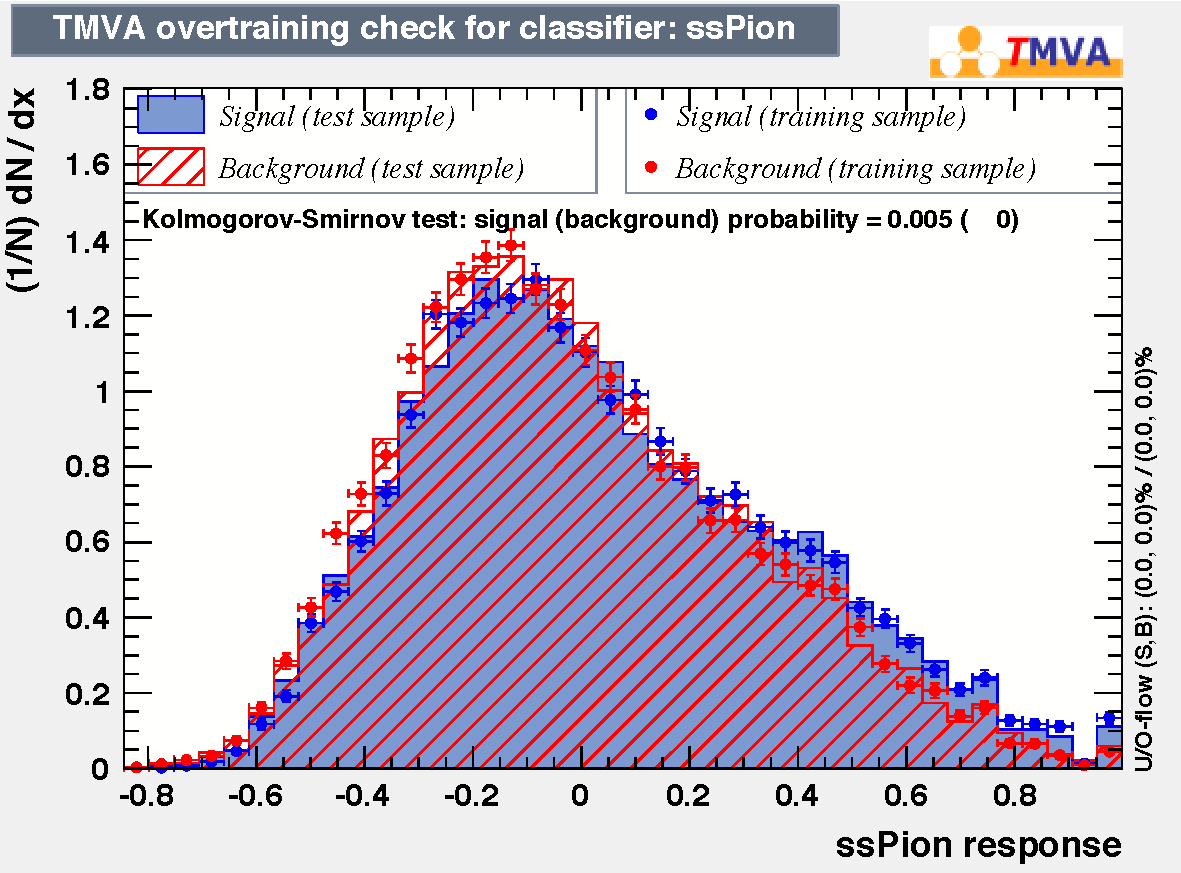
\includegraphics[width=0.6\textwidth]{08FlavourTagging/figs/SSProton_overtrain.pdf}
	\end{center}
	\caption{Output of the SS proton BDT ($\alpha^{\text{SS}\proton}_\text{BDT}$).
	The blue distribution represents the right charge correlated tracks while the red distribution corresponds to the wrong charge correlated tracks.}
	\label{fig:SSProtonBDTOutput}
\end{figure}
Again, a small but significant separation power of the BDT can be seen.
In addition, the test and training samples show some small differences, which probably are a result of a slight overtraining.
However, possible effects arrising due to this are corrected when transforming and calibrating the BDT response.
As for the SS pion algorithm, in case of multiple tagging-proton candidates per event the tag decision and the mistag are defined by the candidate with the largest BDT output.

To determine the relation between the mistag and the BDT output, a time-dependent mixing analysis is performed.
This means, an unbinned maximum-likelihood fit to the distribution of the decay-time $t$, the tag decision $d$ and the mixing state $\xi$ is done.
Since the \emph{sWeigthed} distributions are used for the fit again, only the signal component must be described with the PDF from \cref{eq:mixPDF}.
Firstly the functional relation between the mistag and $\alpha^{\text{SS}\proton}_\text{BDT}$ is determined with a binned fit in the BDT output $\alpha^{\text{SS}\proton}_\text{BDT}$.
Again a $3^{\text{rd}}$ order polynomial as described in \cref{eq:tranformfunc} describes the data well.
An unbinned fit, in which the mistag is parametrised directly in the PDF, finally provides the final transformation parameters, which can be found in \cref{tab:transformSSProton}.
\begin{table}[tbp]
	\centering
	\caption{Final transformation parameters for the BDT response of the SS proton tagger.}
	\begin{tabular}{cccc}
		\toprule
		$b_0$ & $b_1$ & $b_2$ & $b_3$ \\
		\midrule
		\num{0.479\pm0.004} & \num{-0.097\pm0.016} & \num{0.009\pm0.043} & \num{-0.215\pm0.064} \\
		\bottomrule
	\end{tabular}
	\label{tab:transformSSProton}
\end{table}
Figure \ref{fig:MixasymmetrieSSProton} shows the time-dependent mixing asymmetry for the SS proton tagger, the transformation functions of the binned and unbinned approach are presented in \cref{fig:transformationSSProton}.
\begin{figure}[tbp]
	\begin{center}
		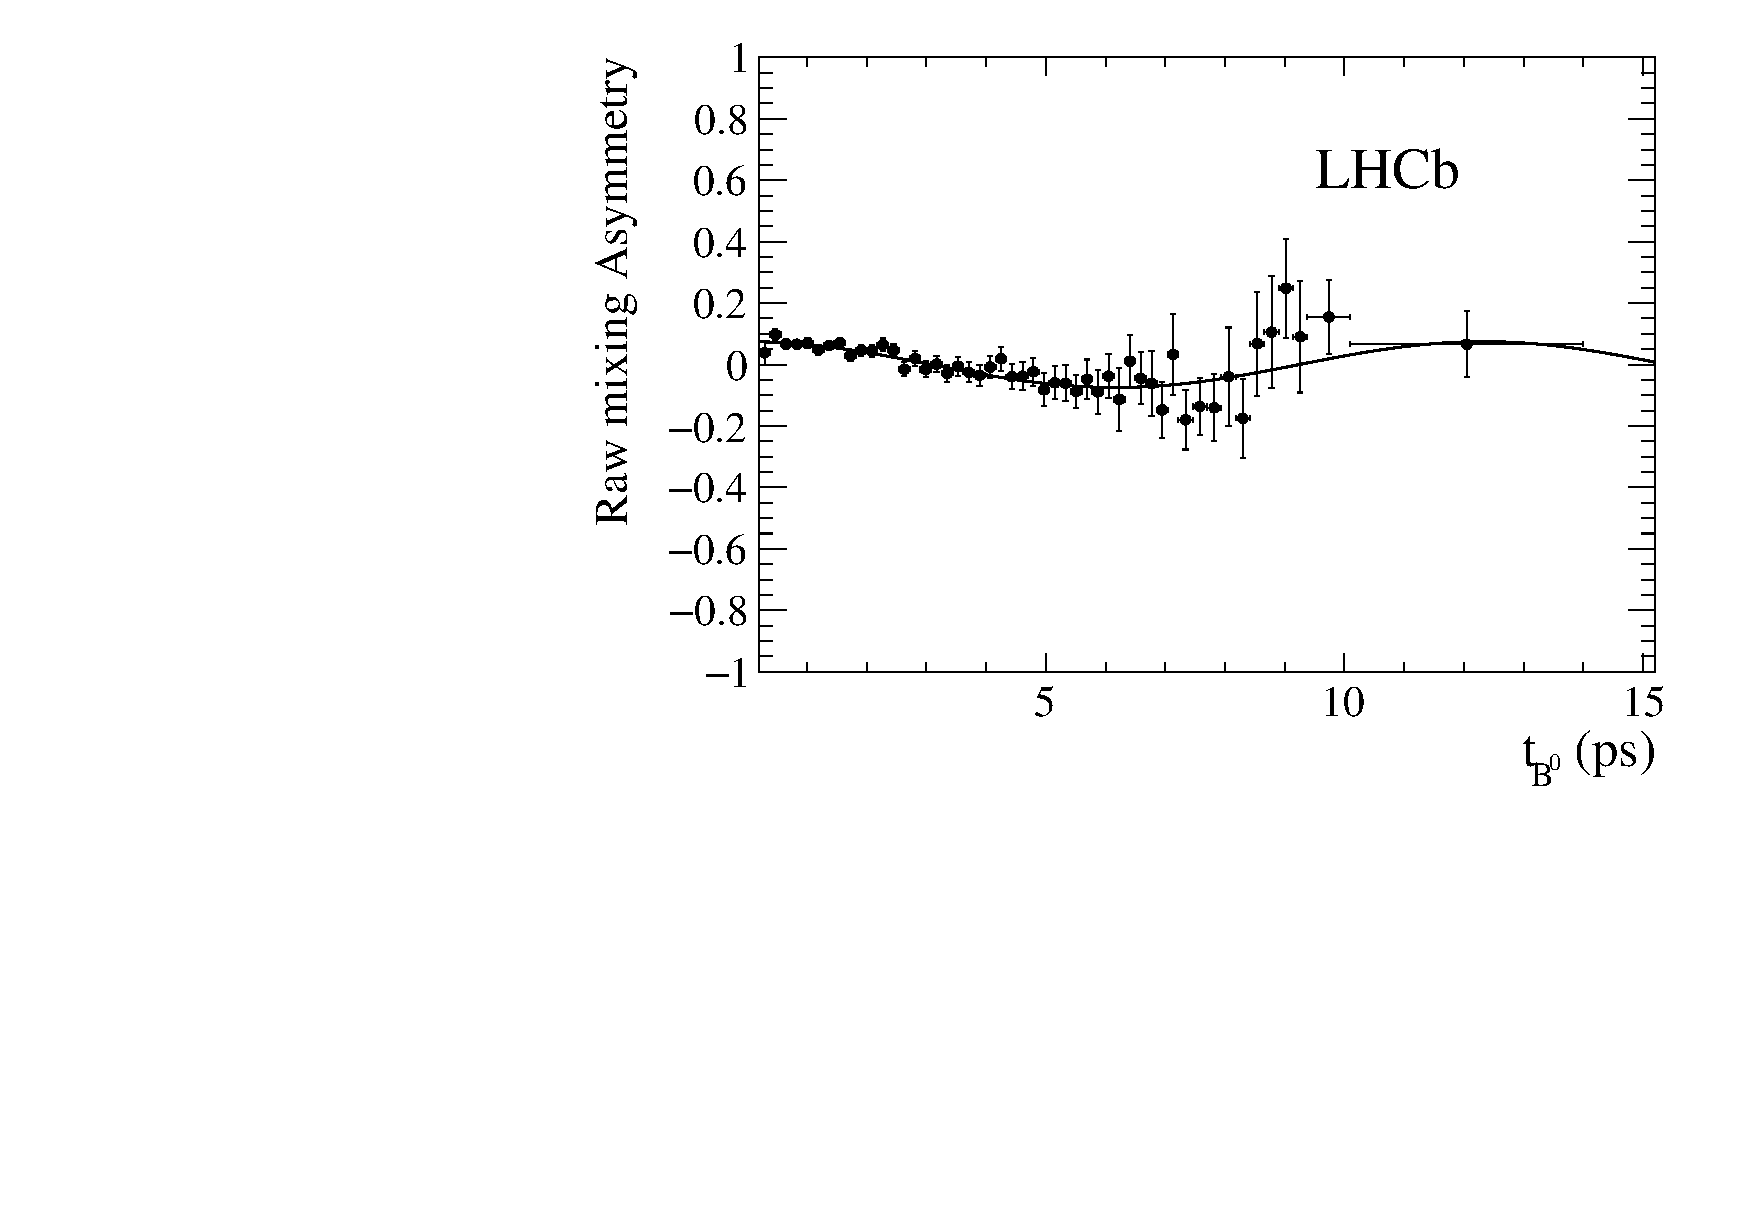
\includegraphics[width=0.6\textwidth]{08FlavourTagging/figs/Asymmetry_SSProton.pdf}
	\end{center}
	\caption{Mixing asymmetry for $\Bz\!\to\jpsi\Kstarz$ candidates tagged by the SS proton tagger.
	The curve overlaid is the fit projection of the decay-time fit.}
	\label{fig:MixasymmetrieSSProton}
\end{figure}
\begin{figure}[tbp]
	\begin{center}
		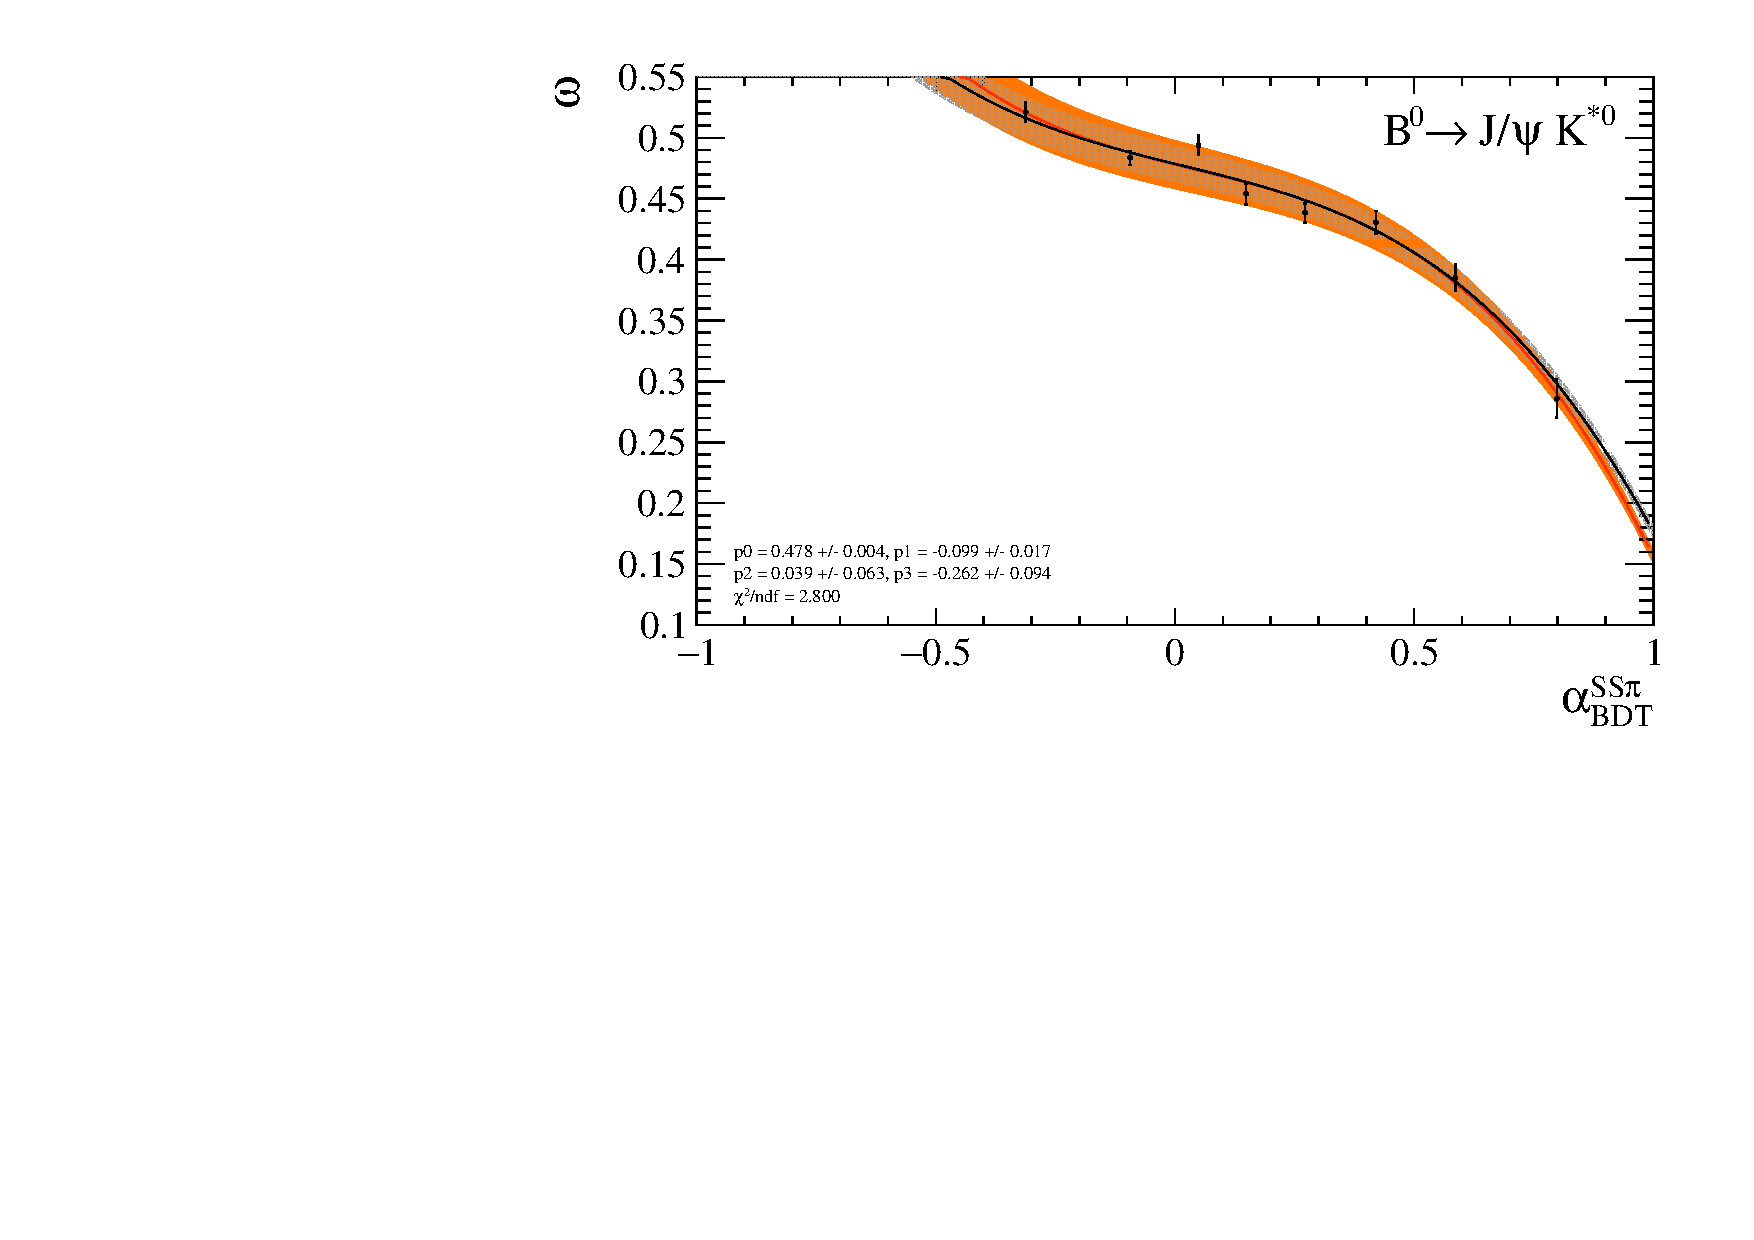
\includegraphics[width=0.6\textwidth]{08FlavourTagging/figs/SSProtonBDTTrafo.pdf}
	\end{center}
	\caption{Polynomial curve of $\omega$ versus $\alpha^{\text{SS}\proton}_\text{BDT}$ on the first two thirds of the $\Bz\!\to\jpsi\Kstarz$ data sample.
	The fit from the binned approach is shown in orange, the curved of the nominal unbinned method is shown in grey.
	The parameter values in the plot correspond to the orange curve/binned approach.}
	\label{fig:transformationSSProton}
\end{figure}

Subsequently, the mistag $\eta$ is then determined using the parameterisation from \cref{tab:transformSSProton}
If the calculated mistag $\eta'$ is greater than \num{0.5}, the tag decision is inverted and the mistag is calculated as $\eta=1-\eta'$.

\subsection{Calibration of the SS tagger combination}
\label{sec:SScombinationcalibration}

After training the taggers of the same side in \cref{sec:retrainSSpion} and \cref{sec:retrainSSproton} they need to be combined.
This is achieved using the formalism from \cref{sec:CombAndCalib}, yielding one global SS tagger with a tag decision $dS{\text{\tiny SS}}$ and a mistag $\eta^{\text{\tiny SS}}$.

This global SS combination then needs to be calibrated.
In order to do this the adopted model is a GLM with a $1^{\text{st}}$ order polynomial as \emph{basis function} and the modified logistic function from \cref{eq:modlink} as \emph{link function}.
The number of free parameters (\num{4}) in the model was selected to achieve several satisfactory goodness-of-fit (GOF) metrics.
The comparisons of GOF metrics are shown in Table \cref{tab:GOFSS}.
\begin{table}[tbp]
        \centering
        \caption{GOF metrics for two different calibration models for the SS taggers.}
        \begin{tabular}{SSS}
                \toprule
                {GOF metric} & {Score (\num{4} parameters)} & {Score (\num{6} parameters)}\\
                \midrule
                {$\chi^2$} 	& 3.3214 & -2.0864 \\
                {$G^2$} 	& 2.5524 & -2.6624 \\
                {$CR$} 		& 3.1819 & -2.7763 \\
                {$S$} 		& 1.5426 & -2.3908 \\
                \bottomrule
        \end{tabular}
        \label{tab:GOFSS}
\end{table}
Since the deviance $G^2$ and the le Cessie-van Houwelingen-Copas-Hosmer metric ($S$) seem to prefer the more simple model, while the Pearson $\chi^2$ and the Cressie-Read ($CR$) metric prefer the more complicated model, both are assumed to fit the data equally well and the more simple one is chosen (all metrics are described in Ref.~\cite{GOFmetric}).
The Calibration is then performed using the \emph{sWeights} together with the weights from \cref{sec:PrepBd2JpsiKstSample}, giving the calibration parameters shown in \cref{tab:CalibSS}.
A graphical representation can be found in \cref{fig:CalibSS}.
\begin{table}[tbp]
	\centering
	\caption{SS calibration parameters obtained on the last third of the $\Bz\to\jpsi\Kstarz$ data sample.}
	\begin{tabular}{cccc}
		\toprule
		$p_0$ & $p_1$ & $\Delta p_0$ & $\Delta p_1$ \\
		\midrule
		\num{-0.091\pm0.059}  & \num{-0.027\pm0.065} & \num{0.034\pm0.084} &\num{0.032\pm0.094}\\
		\bottomrule
	\end{tabular}
	\label{tab:CalibSS}
\end{table}
\begin{figure}[tbp]
	\begin{center}
		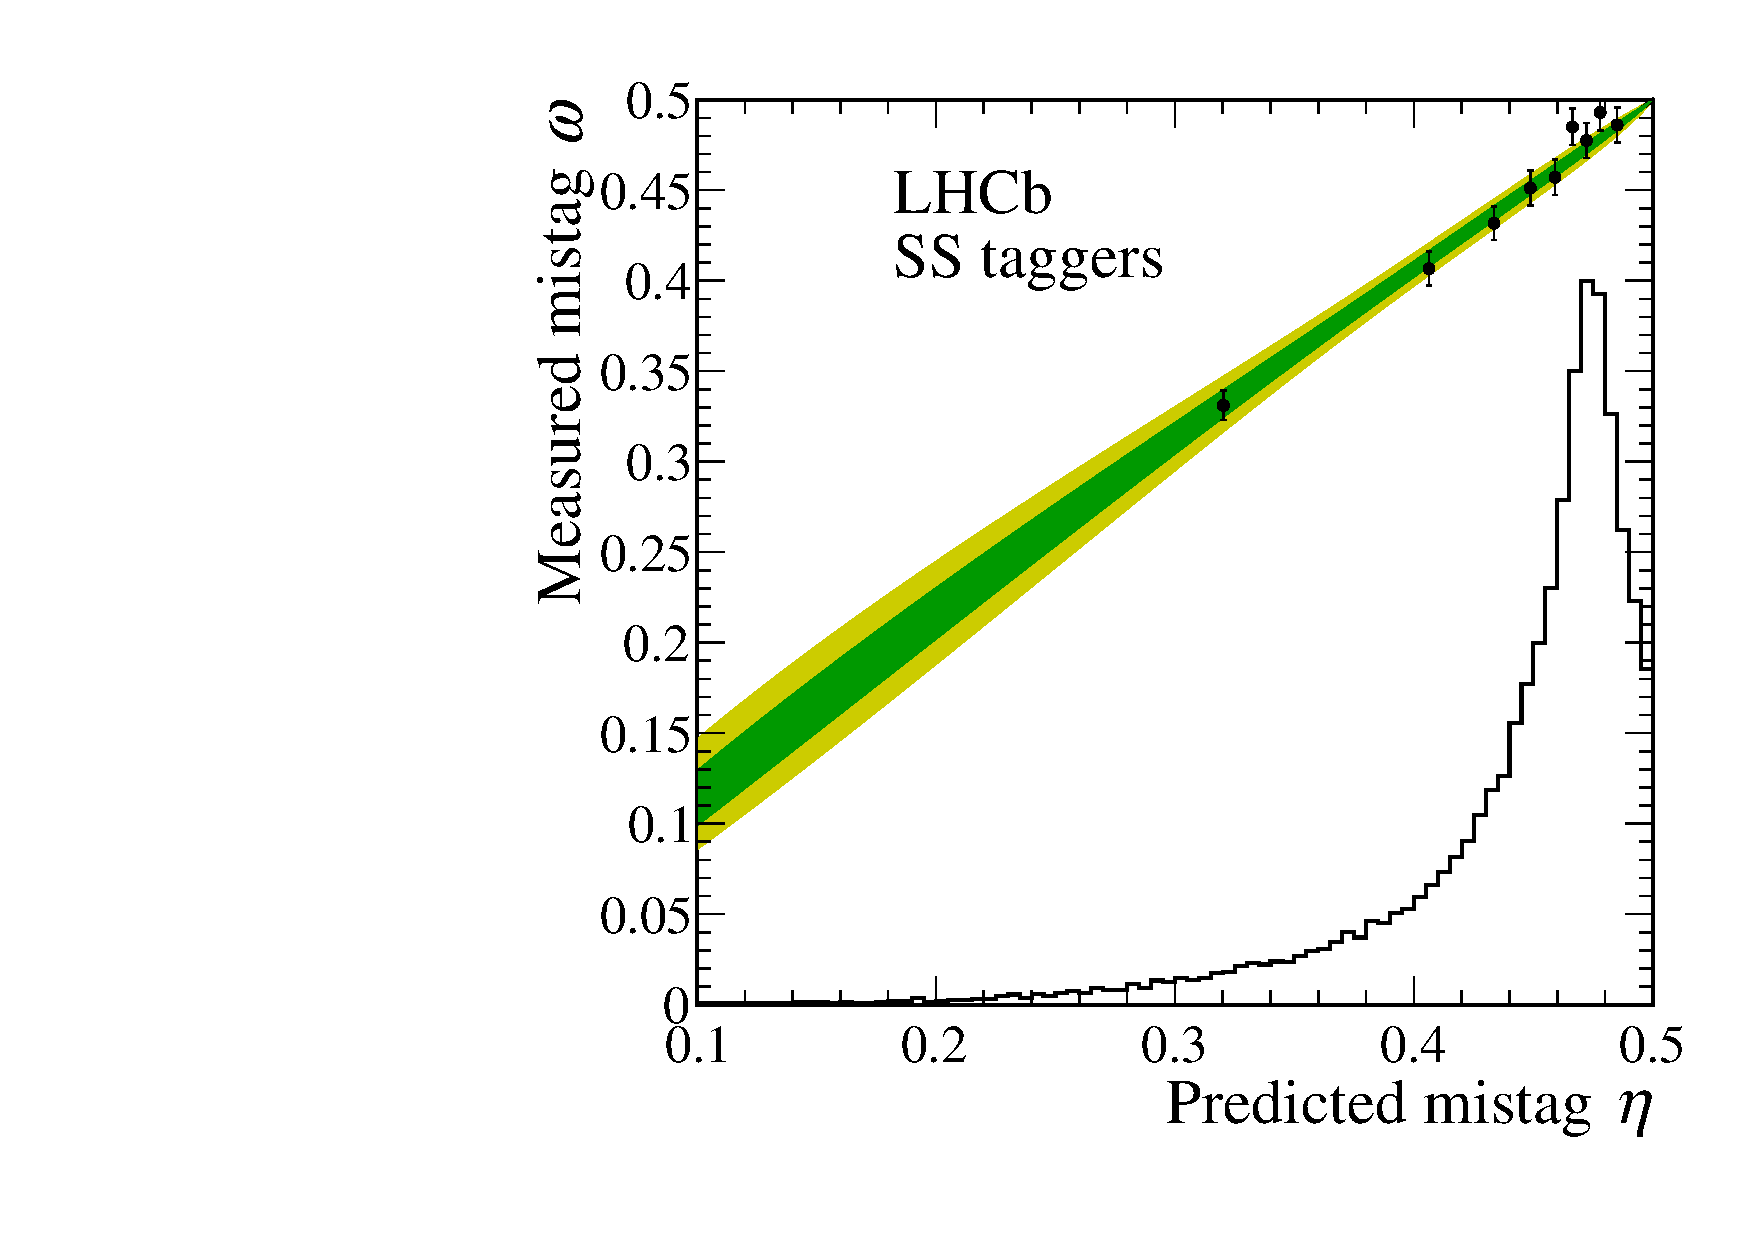
\includegraphics[width=0.45\textwidth]{08FlavourTagging/figs/CalibrationSS.pdf}
	\end{center}
	\caption{Calibration retreived for the SS tagger combination.
	The black histogram is the distributions of the mistag probabilities in arbitrary units.
	The green areas correspond to the \SI{68}{\percent} and \SI{95}{\percent} confidence level regions of the calibration functions.}
	\label{fig:CalibSS}
\end{figure}

The portability of the SS tagger combination is tested on simulated \BdToDpi and $\Bz\!\to\jpsi\Kstarz$ candidates.
This is done using the simulated truth information such that the calibration can be performed in the same way as on a charged decay mode, after equalising the number of initial \Bz- and \Bzb-mesons to separate tagging asymmetries from asymmetries due to \CP-violation or production asymmetries.
Both, the individual calibration parameters and a \enquote{full} comparison from a $\chi^2$ test including the correlations between the parameters, show good agreement (\eg $0.09\sigma$ for the full test).
Despite this good agreement, the parameters in the \CP-fit on \BdToDpi are left free.
On the one hand, this is  motivated by the higher accuracy fo the calibration parameters of the \BdToDpi data sample.
On the other hand this strategy matches the approach for the OS tagger combination, where the portability is not given (\cref{sec:OScalibration}).
In addition, this approach does not require any systematic uncertainty accounting for the portability of the calibration parameters.

\section{Opposite side tagging calibration}
\label{sec:OScalibration}

As mentioned before, the work in this section was done by a collaborator and therefore the explanations will be less detailed than in most other parts of this thesis.

As control channel for the OS tagger combination (namely the OS muon, OS electron, OS kaon, OS vertex charge and OS charm) the charged decay mode $\Bu\!\to\Dz\pip$ is used.
As this decay mode is kinematically  similar to the signal decay \BdToDpi, the same trigger requirements can be applied with a high signal efficiency.
The $\Bu\!\to\Dz\pip$ candidates are further selected by simple rectangular cuts on track quality variables, PID variables, the decay time of the \B-candidate and the invariant mass of the \Dz.
Then a fit to the invariant \Bu mass is performed to extract \emph{sWeights} using the same strategy as in \cref{ch:massfit}.
The invariant mass distribution overlaid with the fit projection from Fit B is shown in \cref{fig:OStaggerMassFit} while \cref{tab:OStaggerMassFitYields} shows the resulting signal and background yields.
\begin{figure}[tbp]
	\begin{center}
		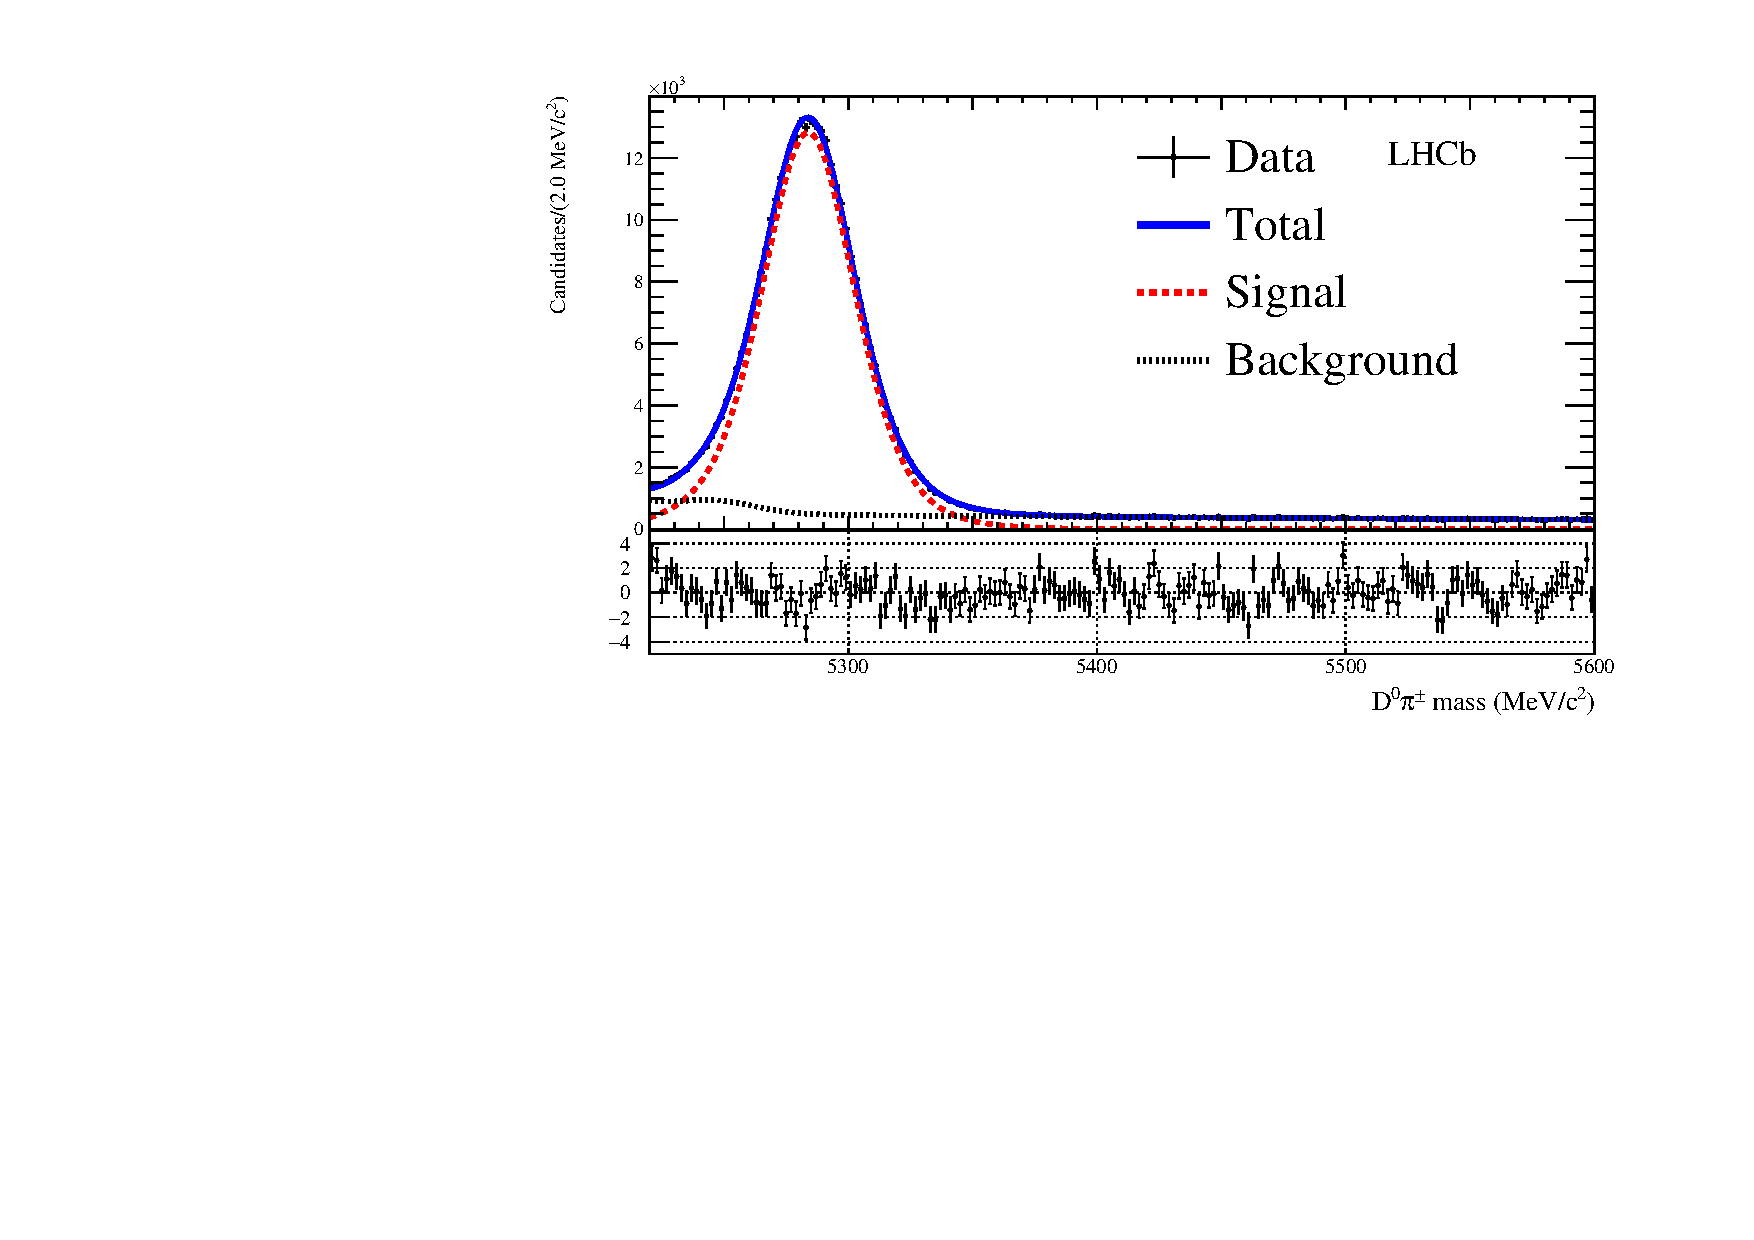
\includegraphics[width=0.7\textwidth]{08FlavourTagging/figs/MDFitForSWeights_BeautyMass_Bu2D0Pi.pdf}
	\end{center}
	\caption{Invariant mass distributions of the $\Dz\pip$ mass.
    The fit projection of Fit B is overlaid.}
	\label{fig:OStaggerMassFit}
\end{figure}
\begin{table}
	\begin{center}
	\caption{Fitted yields of the $\Bu\!\to\Dz\pip$ control channel from Fit B.}
	\begin{tabular}{SS}
		\toprule
		{Parameter} & {Yield} \\
		\midrule
		{$N_{\Bu\!\to\Dz\pip}$}	& 319974\pm612 \\
		{$N_{\text{bkg}}$}		& 85687\pm377 \\
		\bottomrule
	\end{tabular}
	\label{tab:OStaggerMassFitYields}
  \end{center}
\end{table}
Furthermore, the $\Bu\!\to\Dz\pip$ candidates are weighted in the transverse momentum, pseudo-rapidity and decay time of the \B candidate, the number of tracks and PVs in the event and a distribution of trigger decisions to match the distributions of the \BdToDpi candidates.

The calibration model is a GLM with a natural spline function as \emph{basis function} and the modified logistic function from \cref{eq:modlink} as \emph{link function}.
The number of free parameters (\num{10}) in the calibration model is again chosen so that the goodness-of-fit metrics used in \cref{sec:SScombinationcalibration} provide sufficiently satisfactory results.
The comparison with the next simpler model with \num{8} parameters is shown in \cref{tab:GOFOS}.
\begin{table}[tbp]
        \centering
        \caption{GOF metrics for two different calibration models for the OS taggers.}
        \begin{tabular}{SSS}
            \toprule
            {GOF metric} & {Score (8 parameters)} & {Score (10 parameters)} \\
            \midrule
            {$\chi^2$} 	& 4.1312  & -2.197 \\
            {$G^2$} 	& -3.8699 & 0.7199 \\
            $CR$ 		& 2.9273  & -1.6896 \\
            $S$ 		& -4.2701 & 1.8470 \\
            \bottomrule
        \end{tabular}
        \label{tab:GOFOS}
\end{table}
The Calibration is performed using the \emph{sWeights} together with the weights calculated before such that the $\Bu\!\to\Dz\pip$ distributions match the \BdToDpi ones, giving the calibration parameters shown in \cref{tab:CalibOS}.
A graphical representation can be found in \cref{fig:CalibOS}.
\begin{table}[tbp]
	\centering
	\caption{OS calibration parameters obtained on the $\Bu\!\to\Dz\pip$ data sample.}
	\begin{tabular}{ccccc}
		\toprule
		$p_0$ & $p_1$ & $p_2$ & $p_3$ & $p_4$ \\
		\midrule
		\num{-0.136\pm0.019}  & \num{-0.006\pm0.022} & \num{-0.0107\pm0.0083} &\num{-0.45\pm0.10} &\num{-0.85\pm0.46}\\
		\midrule
		$\Delta p_0$ & $\Delta p_1$ & $\Delta p_2$ & $\Delta p_3$ & $\Delta p_4$ \\
		\midrule
		\num{-0.129\pm0.038}  & \num{0.042\pm0.045} & \num{-0.020\pm0.017} &\num{0.42\pm0.21} &\num{1.91\pm0.92}\\
		\bottomrule
	\end{tabular}
	\label{tab:CalibOS}
\end{table}
\begin{figure}[tbp]
	\begin{center}
		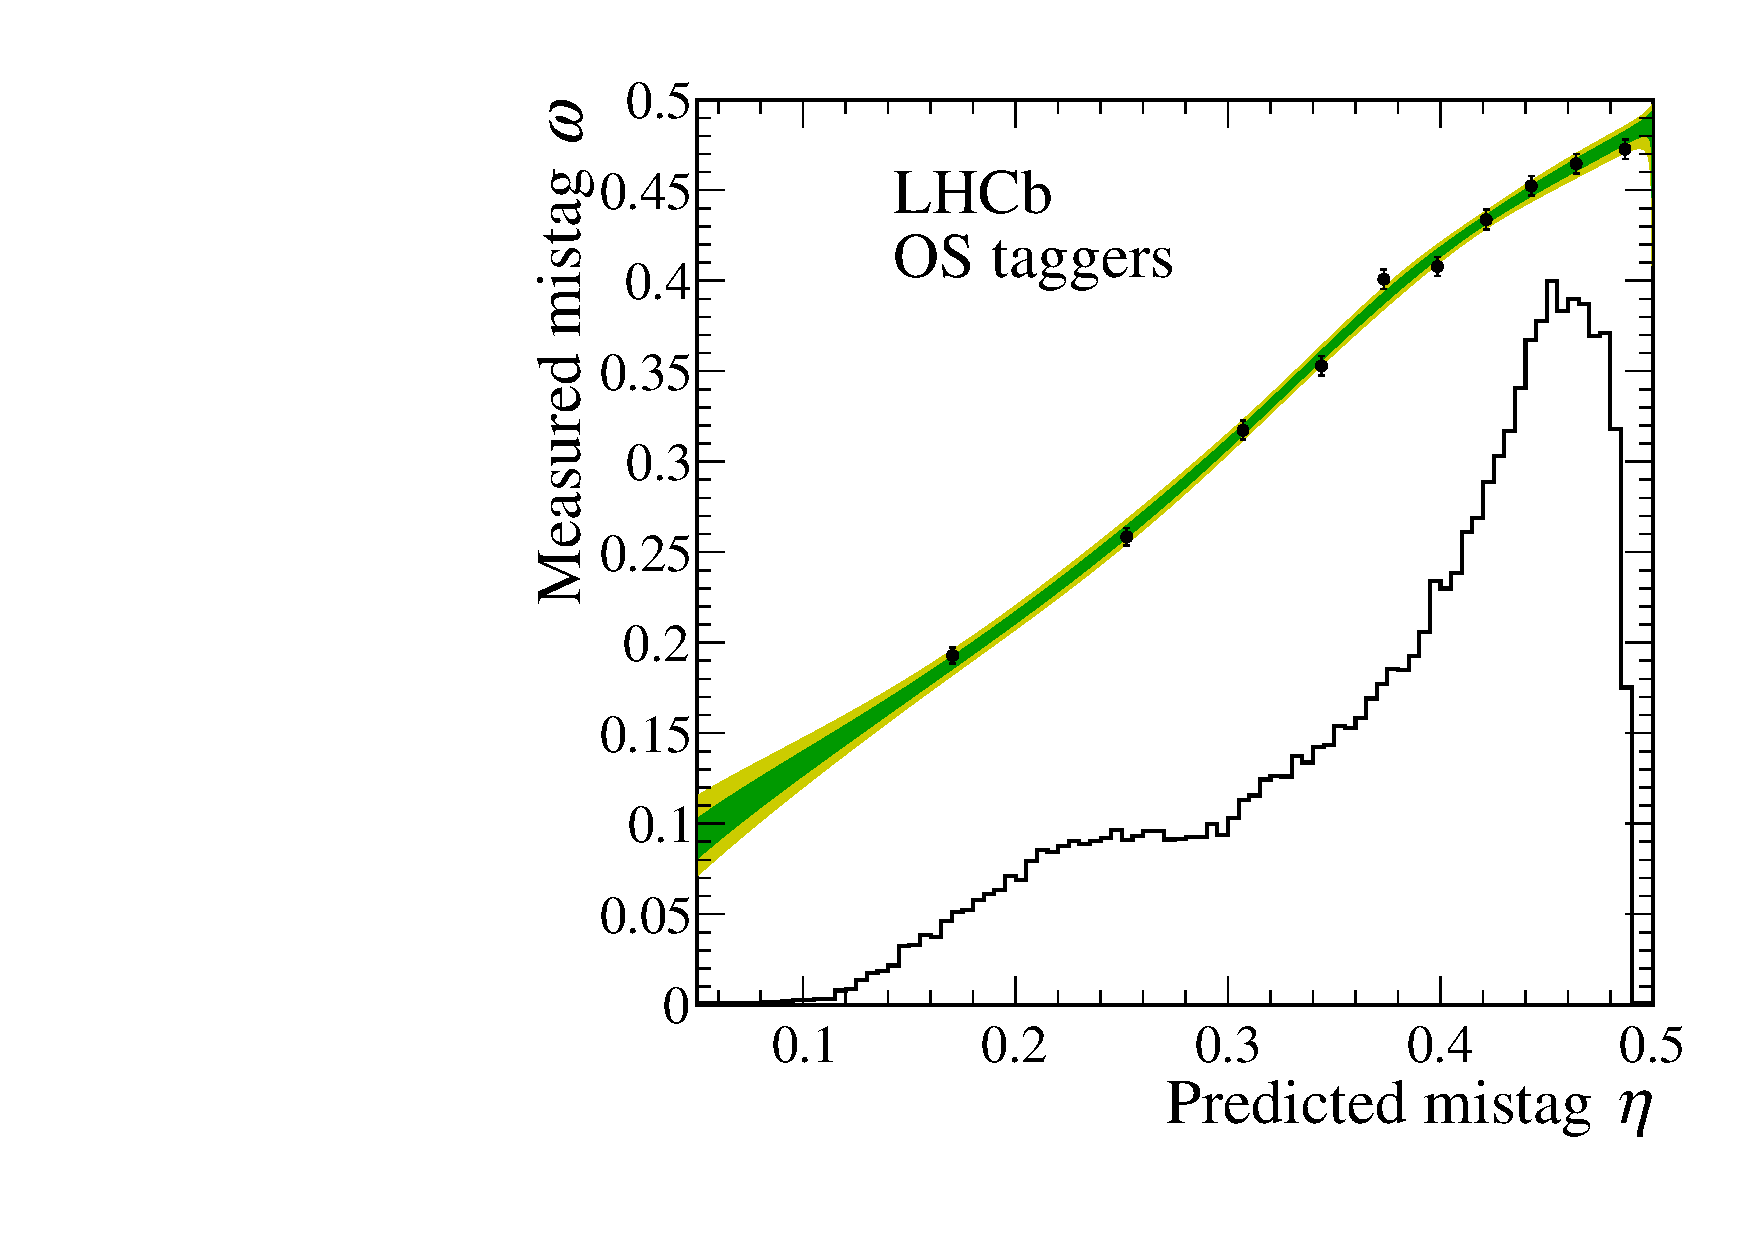
\includegraphics[width=0.45\textwidth]{08FlavourTagging/figs/CalibrationOS.pdf}
	\end{center}
	\caption{Calibration retreived by the for the OS tagger combination.
	The black histogram is the distributions of the mistag probabilities in arbitrary units.
	The shaded areas correspond to the \SI{68}{\percent} and \SI{95}{\percent} confidence level regions of the calibration functions.}
	\label{fig:CalibOS}
\end{figure}

The portability of the calibration is checked on simulated candidates.
The calibration is determined using the simulated true initial flavours on both decay channels after equalising the number of initial \Bz (\Bu) and \Bzb (\Bm) mesons.
The parameters $p_0$ and $p_1$ show deviations of more than $2.5\sigma$, while the full comparison taking into account the correlations between the parameters shows a discrepancy of $2.0\sigma$.
Although one could presume this overall discrepancy is sufficiently small, a study on simulated events presented in \cref{sec:decTimeFitVal} shows that applying the calibration determined on $\Bu\!\to\Dz\pip$ causes a bias for the \CP-parameters \Sf and \Sfbar.
Presumably some residual discrepancies remain despite the weighting of the $\Bu\!\to\Dz\pip$ candidates.
For this reason, the portability is not considered to be given and the calibration is determined directly in the \CP fit on \BdToDpi.

  % % !TEX root = main.tex
\chapter{Decay-time fit}

In this chapter the decay-time fit on \BdToDpi to extract the \CP observables \Sf and \Sfbar is presented.
Section \ref{sec:resolution} and \ref{sec:acceptance} describe the parameterisation of the decay time resolution and acceptance before the extraction of the \CP parameters is presented in \cref{sec:ExtractCPobs}.
Following, this fit needs to be validated.
This can be achieved by first comparing the resulting values of nuisance parameters with reference values.
Further the \emph{link function} used for the calibration function of the OS and SS taggers needs to be validated (\cref{sec:ValLinkFunction}).
At last, the fit to extract the CP parameters is repeated on different subsamples of the data set (\cref{sec:valOnSubSample}) and the entire strategy is also checked on simulated events (\cref{sec:valOnSim}).

\section{Fit to data}

In the following the last preparatory studies and the decay-time fit to extract \Sf and \Sfbar are presented.
The fit is performed on the decay-time range from \SIrange{0.4}{12}{\pico\second}.
This lower limit was chosen in order to obtain a good description of the decay-time distribution at low decay-times without losing sensitivity on the parameters \Sf and \Sfbar.
The upper limit was set to a value such that the statistics is already too small so that an enlarged range would no longer be useful to add sensitivity on the \CP parameters.

\subsection{Decay time resolution}
\label{sec:resolution}

Since the work in this section was done by a collaborator, the contents are described for the sake of completeness, but smaller details are omitted.

The decay-time resolution is determined on a sample of \emph{fake} \Bz-candidates, formed from a prompt \Dpm candidate and another track originating from the PV.
The candidates are selected with the same selection as presented in \cref{sec:selection}, except for the cut on the BDT output.
Additionally, the \emph{fake} \Bz-candidates are required to have an impact parameter $\chi^2$ with the PV less than nine and the number of \ac{PV}s in the event must be one to exclude wrong \ac{PV} associations.
Subsequently \emph{sWeights} are determined by a fit to the invariant mass of the \Dpm meson in order to examine only signal distributions in the following.
Since the time resolution depends on the transverse momentum of the bachelor particle, as a last preparatory step, this need to be corrected in the sample of \emph{fake} \Bz-candidates.
Therefore the prompt sample is weighted by the ratio of the distributions of the logarithmic transverse momenta of the bachelor candidate in the signal \BdToDpi and the prompt sample.

To resolve the decay-time resolution, fits are then performed to the decay-time distribution of the prompt sample in \num{20} bins of the decay-time error.
Since this sample does not contain real \Bz candidates, the decay time is expected to be zero and the decay-time resolution can be derived from the width of the distribution.
The binning is chosen so that the sum of \emph{sWeights} in each bin is equal.
The fit model consists of three components: A delta function convolved with a Gaussian function to describe the true \Dpm+track component, a pair of exponential functions convolved with the same Gaussian function to describe candidates from \bquark-hadron and a wide Gaussian function to describe backgrounds due to wrongly associated \ac{PV}s.
The fit is shown for one representative bin in \cref{fig:resolutionRepresentativeBin}.
\begin{figure}[tbp]
    \centering
    \includegraphics[width=0.48\textwidth]{09TimeFit/figs/resolution_Bin15.pdf}
    \includegraphics[width=0.48\textwidth]{09TimeFit/figs/resolution_chi2Fit.pdf}
    \caption{Left: Decay-time resolution for one representative bin in per-candidate decay-time error for \emph{fake} \Bz candidates.
    Right: Measured resolution versus average per-candidate decay-time error, determined from fits to the decay time in bins of decay-time error.}
    \label{fig:resolutionRepresentativeBin}
\end{figure}
A measured resolution $\left<\sigma\right>_i$ per bin is obtained from this fit, which can be related to the corresponding average decay-time error $\left<\delta\right>_i$.
Following a $\chi^2$ is fit to the $(\left<\delta\right>_i, \left<\sigma\right>_i)$ pairs of the form
\begin{equation}
\left<\sigma\right>_i=\left<\sigma\right>+p_1\times\left(\left<\delta\right>_i-\left<\delta\right>\right)+p_2\times\left(\left<\delta\right>_i-\left<\delta\right>\right)^2
\end{equation}
is performed, where $\left<\delta\right>$ is the average per-event decay-time error of the whole unbinned sample.
This $\chi^2$ fit is shown in \cref{fig:resolutionRepresentativeBin}.
It provides an average decay time resolution $\left<\sigma\right>$ and a trend, from which a global average resolution of \mbox{$\sigma\!\left(\left<\delta\right>\right)=\SI{54.91\pm0.38}{\femto\second}$} can be determined.

\subsection{Decay-time dependent efficiency}
\label{sec:acceptance}

Due to some selection criteria and trigger requirements, as well as inefficiencies in \velo reconstruction, the detector efficiency is not constant over the \Bz decay-time.
This efficiency, hereinafter referred to as acceptance, decreases very quickly towards zero for low decay times, reaches a plateau for intermediate decay times, and slightly drops again at high decay times.

For this analysis two models were developed in parallel, which give almost identical results for the \CP parameters \Sf and \Sfbar.
The model used in the final decay-time fit was developed by a collaborator and has one degree of freedom more, while the model described below is used as a crosscheck and for estimating systematic uncertainties.
In both models the acceptance is defined by splines, which are defined analytically in the decay-time fit as described in Ref.~\cite{Karbach:2014qba}.
These splines consist of cubic polynomials defined piecewise in decay-time.
The model is then defined by the limits of the ranges on which the cubic polynomials are defined (also denoted as knots) and associated coefficients.

The parameterisation described below belongs to the second model developed by myself.
The model is optimised in order to find the ideal knot  positions giving a good descirption of the decay-time with the minimum number of knots at the same time.
This is done on simulated events by performing a maximum-likelihood fit to the decay-time with the PDF defined as
\begin{equation}
\mathcal{A}(t)\propto a(t)\int dt' \mathcal{R}\!\left(t-t'\right)e^{\,\nicefrac{t'}{\tau}}
\end{equation}
where the resolution $\mathcal{R}\!\left(t-t'\right)$ is taken from \cref{sec:resolution} and the lifetime $\tau$ is fixed to the value used in the generation.
It is further checked if the obtained model also describes the \emph{sWeighted} decay-time distribution in the \BdToDpi sample satisfactorily.
Instead of fixing the lifetime on data it is constraint by means of a Gaussian function to the world average $\tau=\SI{1.518\pm0.004}{\pico\second}$~\cite{PDG_2017}.
A good description was found using seven knots at $[0.4, 0.45, 0.8, 1.3, 2.5, 6.0, 12.0]\,$\si{\pico\second}, where the coefficient at \SI{2.5}{\pico\second} is set to one to fix the overall normalisation.
Figure \ref{fig:acceptance} shows a graphical representation of the used parameterisation with the coefficients obtained on \BdToDpi data (the numerical values of the coefficients are given in \cref{tab:acceptance}).
\begin{figure}[tbp]
    \centering
    \includegraphics[width=0.7\textwidth]{09TimeFit/figs/Acceptance.pdf}
    \caption{Graphical representation of the acceptance for \BdToDpi.
    The dotted vertical lines represent the knot positions, the dashed lines show the underlying cubic polynomials, where the same colour is chosen for the associated knot and polynomial.}
    \label{fig:acceptance}
\end{figure}
\begin{table}[tbp]
	\centering
	\caption{Spline coefficients $v_i$ as obtained for the decay-time distribution on \BdToDpi.
	As stated in the text the coefficient $v_5$ is set to one, to fix the overall normalisation.}
	\begin{tabular}{SS}
		\toprule
		{Parameter} & {Value} \\
		\midrule
		{$v_1$} 	& 0.187\pm0.004 \\
		{$v_2$} 	& 0.306\pm0.005 \\
		{$v_3$} 	& 0.557\pm0.005 \\
		{$v_4$} 	& 0.870\pm0.010 \\
		{$v_6$} 	& 0.880\pm0.023 \\
		{$v_7$} 	& 0.759\pm0.023 \\
		\bottomrule
	\end{tabular}
	\label{tab:acceptance}
\end{table}

\subsection[head={Extraction of \CP observables},tocentry={Extraction of \CP observables}]{Extraction of $\symbfsf{\CP}$ observables}
\label{sec:ExtractCPobs}

The \CP parameters \Sf and \Sfbar are determined through a multidimensional unbinned maximum-likelihood fit to the by \emph{sWeights} background-subtracted distributions of \BdToDpi.
The PDF to describe the decay time $t$, the tags $\vec{d}=(d^{\text{\tiny OS}}, d^{\text{\tiny SS}})$ and the final state $F$ taking the values \f and \fbar, given the mistags $\vec{\eta}=(\eta^{\text{\tiny OS}}, \eta^{\text{\tiny SS}})$ is defined by
\begin{equation}
\mathcal{P}(t, F, \vec{d}|\vec{\eta})\propto a(t)\left(P(t', F, \vec{d}|\vec{\eta})\otimes R(t'-t)\right)\label{eq:FinalDecayTimePDF}
\end{equation}
where $P(t', F, \vec{d}|\vec{\eta})$ describes the true decay time, $R(t'-t)$ is the resolution from \cref{sec:resolution} and $a(t)$ parametrises the acceptance described in \cref{sec:acceptance}.
Furthermore the function $P(t', F, \vec{d}|\vec{\eta})$ corresponds to the decay rates from \crefrange{eq:DecRateB2Dmpip}{eq:DecRateBb2Dppim}, taking into account the corrections from \cref{eq:decRateCorrectFT}.
Besides, production and detection asymmetry must be described.
These are defined as
\begin{equation}
A_{\text{P}}=\frac{\sigma(\Bzb)-\sigma(\Bz)}{\sigma(\Bzb)+\sigma(\Bz)}\hspace{0.5cm}\text{and}\hspace{0.5cm}A_{\text{D}}=\frac{\varepsilon(\,\f)-\varepsilon(\,\fbar)}{\varepsilon(\,\f)+\varepsilon(\,\fbar)}
\end{equation}
where $\varepsilon$ is the decay time integrated reconstruction and selection efficiency for the finalstates \f and \fbar and $\sigma$ is the production cross-section for \Bz and \Bzb mesons.
Both asymmetries were determined to be at the percent level in independent measurements at \lhc energies.
As both are further known to be decay-time independent they can be described by modifying the expressions for the \CP coefficients from \cref{eq:decRateCorrectFT} further to
\begin{equation}
\begin{aligned}
\left(\Delta^--\Delta^+\right)\Sf&\to\left(\Delta^--A_{\text{P}}\,\Delta^+\right)(1+A_{\text{D}})\Sf\\
\left(\Delta^--\Delta^+\right)\Cf&\to\left(\Delta^--A_{\text{P}}\,\Delta^+\right)(1+A_{\text{D}})\Cf.
\end{aligned}
\end{equation}
The same expressions also apply to \Sfbar and \Cfbar with the substitution $A_{\text{D}}\to -A_{\text{D}}$.

As explained in \cref{sec:taggingstrategy}, due to the expected small value of $r$ (see \cref{sec:GammaInBd2Dpi}), the parameters \Cf and \Cfbar are fixed to \num{1} and \num{-1}.
Moreover, since possible tagging efficiency asymmetries are measured in simulation to be compatible with zero, they are fixed to this value for the OS and SS taggers.
Possible systematic effects due to one of both assumptions are taken into account in the systematic uncertainties.
Furthermore, the following parameters are constrained by means of a Gaussian function:
\begin{equation}
\begin{aligned}
\tau&=\SI{1.518\pm0.004}{\pico\second}\\
\dm&=\SI{0.5050\pm0.0023}{\per\pico\second}.
\end{aligned}
\end{equation}
For the lifetime $\tau$ the world average~\cite{PDG_2017} is taken and for the oscillation frequency \dm the result of the semi-leptonic \lhcb measurement~\cite{Aaij:2016fdk} is used.
Hence, the free parameters in the fit are the \CP parameters \Sf and \Sfbar, the production and detection asymmetry, the calibration parameters of the OS and SS taggers and the acceptance parameters.
The fitted values for the parameters \Sf, \Sfbar, \dm, \DG, $A_{\text{P}}$ and $A_{\text{P}}$ are shown in \cref{tab:DecTimeProjection}, \cref{fig:DecTimeProjection} shows the projection of the PDF onto the decay-time distribution.
For the \CP parameters \Sf and \Sfbar it is important to note that the given uncertainties are not purely statistical, but also include the systematic contributions from \dm and $\tau$ via the applied constraints.
Repeating the fit with \dm and $\tau$ fixed to the central values of the constraints, the central values for \Sf and \Sfbar stay unchanged, but the uncertainties decrease to \num{0.020}.
\begin{figure}[tbp]
    \centering
    \includegraphics[width=0.7\textwidth]{09TimeFit/figs/BeautyTime_pull.pdf}
    \caption{Background-subtracted decay-time distribution of \BdToDpi candidates.
    The solid curve is the projection of the PDF, the black points represent the data.
    The lower histogram shows the distributions of pulls, \ie the difference of the binned data and the fitted PDF divided by the data uncertainty in each bin.}
    \label{fig:DecTimeProjection}
\end{figure}

\begin{table}[tbp]
	\centering
	\caption{Fit results for \Sf, \Sfbar, \dm, \DG, $A_{\text{P}}$ and $A_{\text{D}}$ from the nominal decay-time fit in \BdToDpi.
	The uncertainties on \Sf and \Sfbar are not purely statistical, but contain the systematic contributions from the constraints on \dm and $\tau$.}
	\begin{tabular}{SS[table-format=1.4]@{\,\( \pm \)\,}S[table-format=1.4]@{\,}s[table-unit-alignment = left]}
		\toprule
		{Parameter} & \multicolumn{3}{c}{\kern -1.1cm Value}  \\
		\midrule
		{\Sf} 				& 0.058 & 0.021 \\
		{\Sfbar} 			& 0.038 & 0.021 \\
		{\dm} 				& 0.5054 & 0.0022 & \si{\per\pico\second} \\
		{$\tau$} 			& 1.5180 & 0.0040 & \si{\pico\second} \\
		{$A_{\text{P}}$} 	& -0.0064 & 0.0028 \\
		{$A_{\text{D}}$} 	& 0.0086 & 0.0019 \\
		\bottomrule
	\end{tabular}
	\label{tab:DecTimeProjection}
\end{table}
In \cref{fig:AsymProjection} the \CP asymmetries given by
\begin{equation}
\begin{aligned}
A_{\CP}^{\,f}(t)=\frac{\Gamma\!\left(\Bz\!\to\Dm\pip\right)-\Gamma\!\left(\Bzb\!\to\Dm\pip\right)}{\Gamma\!\left(\Bz\!\to\Dm\pip\right)+\Gamma\!\left(\Bzb\!\to\Dm\pip\right)},\\
A_{\CP}^{\,\kern 1.5pt\overline{\kern -1.5pt f\kern 1.5pt}}(t)=\frac{\Gamma\!\left(\Bz\!\to\Dp\pim\right)-\Gamma\!\left(\Bzb\!\to\Dp\pim\right)}{\Gamma\!\left(\Bz\!\to\Dp\pim\right)+\Gamma\!\left(\Bzb\!\to\Dp\pim\right)}
\end{aligned}
\end{equation}
are shown.
However, as these are mainly dominated by the cosine oscillation also the signal-yield asymmetries between candidates tagged as \Bz and \Bzb split according to the favoured (F) $\bquarkbar\!\to\cquarkbar\uquark\dquarkbar$ and the suppressed (S) $\bquarkbar\!\to\uquarkbar\cquark\dquarkbar$ transitions
\begin{equation}
\begin{aligned}
A_{\text{F}}(t)=\frac{\Gamma\!\left(\Bz\!\to\Dm\pip\right)-\Gamma\!\left(\Bzb\!\to\Dp\pim\right)}{\Gamma\!\left(\Bz\!\to\Dm\pip\right)+\Gamma\!\left(\Bzb\!\to\Dp\pim\right)},\\
A_{\text{S}}(t)=\frac{\Gamma\!\left(\Bzb\!\to\Dm\pip\right)-\Gamma\!\left(\Bz\!\to\Dp\pim\right)}{\Gamma\!\left(\Bzb\!\to\Dm\pip\right)+\Gamma\!\left(\Bz\!\to\Dp\pim\right)}\label{eq:AsymeSuppFav}
\end{aligned}
\end{equation}
are presented in \cref{fig:AsymProjection}.
For this asymmetries in addition to the projection of the nominal fit also the projection of an alternative fit assuming no \CP violation, \ie $\Sf=-\Sfbar$, is shown.
\begin{figure}[tbp]
    \centering
    \includegraphics[width=0.48\textwidth]{09TimeFit/figs/Asym_f.pdf}
    \includegraphics[width=0.48\textwidth]{09TimeFit/figs/Asym_fbar.pdf}\\
    \includegraphics[width=0.48\textwidth]{09TimeFit/figs/Asym_favour.pdf}
    \includegraphics[width=0.48\textwidth]{09TimeFit/figs/Asym_suppress.pdf}
    \caption{Top: Decay-time dependent signal yield asymmetry for the \Dm\pip (left) and the \Dp\pim (right) finalstate.
    The solid curve represent the projection of the fitted PDF.
    Bottom: Decay-time dependent signal yield asymmetry for the favoured (left) and the suppressed (right) transitions.
    The asymmetries are defined in \cref{eq:AsymeSuppFav}.
    The blue solid curve is the projection of the fitted PDF from the nominal fit, the red dotted curve shows the projection of a second fit imposing no \CP violation.}
    \label{fig:AsymProjection}
\end{figure}

Using the results of the fitted calibration parameters (the results themselves are discussed in \cref{sec:decTimeFitVal}) and the fitted tagging efficiencies of $\varepsilon_{\text{tag}}^{\text{\tiny OS}}=\SI{43.24\pm0.07}{\percent}$ and $\varepsilon_{\text{tag}}^{\text{\tiny SS}}=\SI{93.05\pm0.04}{\percent}$ the tagging performances in the sample can be computed.
The average dilution is \SI{9.53\pm0.03}{\percent} and \SI{2.789\pm0.009}{\percent} for the OS and SS taggers, respectively.
This leads to an overall average dilution of \SI{6.55\pm0.02}{\percent}.
Also including the untagged candidates which were removed in \cref{ch:massfit}, the total effective tagging efficiency is calculated to be \SI{5.59\pm0.01}{\percent}.

\section{Fit validation}
\label{sec:decTimeFitVal}

To validate the decay-time fit, first it is possible to compare the fitted nuisance parameters like the production and detection asymmetry and the flavour tagging calibration parameters with reference values.
The production and detection asymmetries are directly compared with values from independent measurements from \lhcb.
The results of $A_{\text{P}}=\SI{-0.64\pm0.28}{\percent}$ and $A_{\text{D}}=\SI{0.86\pm0.19}{\percent}$ are well in agreement with the results from Ref.~\cite{Aaij:2017mso}, which \eg range from \SIrange{-1.43\pm0.86}{-0.56\pm0.30}{\percent} for measurements of the production asymmetry at centre-of-mass energies of \num{7} and \SI{8}{\tera\electronvolt} in the decay channels $\Bz\!\to\jpsi\Kstarz$ and $\Bs\!\to\Dsm\pip$.
The obtained calibration parameters are compared to those computed on the control channels $\Bu\!\to\Dz\pip$ and $\Bz\!\to\jpsi\Kstarz$ for the OS and SS, respectively.
In \cref{tab:taggingCalibCompare} the parameters from the decay-time fit in \BdToDpi are listed and the deviation of each parameter with the calibrations given in \cref{tab:CalibSS} and \cref{tab:CalibOS} are calculated.
The largest deviation can be found for $\Delta p_{X}$ and $\Delta p_{Y}$ being of the size of two standard deviations.
Additionally, taking into account the correlations between the parameters an overall discrepancy is calculated yielding $0.91\sigma$ for the OS and $0.29\sigma$ for the SS taggers.
\begin{table}[tbp]
	\centering
	\caption{Calibration parameters obtained in the decay-time fit in \BdToDpi.
	The deviations are calculated with respect to the calibration parameters derived from the control modes $\Bu\!\to\Dz\pip$ (\cref{tab:CalibOS}) and $\Bz\!\to\jpsi\Kstarz$ (\cref{tab:CalibSS}).}
	\begin{tabular}{c|S[table-format=2.3,table-figures-uncertainty=1]S[table-format=1.2]|S[table-format=2.3,table-figures-uncertainty=1]S[table-format=1.2]}
		\toprule
		 & \multicolumn{2}{c|}{OS} & \multicolumn{2}{c}{SS}  \\
		\midrule
		{Parameter} & {Value} & {Deviation} & {Value} & {Deviation} \\
		\midrule
		{$p_0$} 		& -0.152\pm0.021 	& -0.56 & -0.041\pm0.021 & 0.80 \\
		{$p_1$} 		& -0.035\pm0.024 	& -0.89 & -0.012\pm0.022 & 0.22 \\
		{$p_2$} 		& -0.007\pm0.009 	& -0.33 & {-} 			 & {-} \\
		{$p_3$} 		& -0.32\pm0.11 		& 0.90  & {-}			 & {-} \\
		{$p_4$} 		& -0.47\pm0.49 		& 0.57  & {-}			 & {-} \\
		{$\Delta p_0$} 	& -0.079\pm0.049 	& 0.81  & -0.085\pm0.044 & -1.25 \\
		{$\Delta p_1$} 	& 0.140\pm0.036 	& 1.72  & 0.042\pm0.033  & 0.11 \\
		{$\Delta p_2$} 	& -0.024\pm0.013 	& -0.19 & {-} 			 & {-} \\
		{$\Delta p_3$} 	& -0.26\pm0.16 		& -2.66 & {-} 			 & {-} \\
		{$\Delta p_4$} 	& -0.52\pm0.71 		& -2.11 & {-} 			 & {-} \\
		\bottomrule
	\end{tabular}
	\label{tab:taggingCalibCompare}
\end{table}

Next, the two-dimensional contour plots for the \CP parameters \Sf and \Sfbar and for the detection and production asymmetries can be checked.
As shown in \cref{fig:corrPlots} both do not show any unexpected behaviour, only the expected Gaussian ellipses, indicating that the corresponding uncertainties are well understood.
\begin{figure}[tbp]
    \centering
    \includegraphics[width=0.48\textwidth]{09TimeFit/figs/SfvsSfbar.pdf}
    \includegraphics[width=0.48\textwidth]{09TimeFit/figs/ApvsAd.pdf}
    \caption{Contour plot for (\Sf, \Sfbar) (left) and ($A_{\text{P}}$, $A_{\text{D}}$) (right) showing the one, two and three sigma contours.
    The uncertainties include the full statistical uncertaintiy and the systematic uncertainty due to the constraints on \dm and $\tau$.}
    \label{fig:corrPlots}
\end{figure}

\subsection{Validation of link funktion for mistags}
\label{sec:ValLinkFunction}

As mentioned before, the handling of candidates with a mistag close to \num{0.5} is important, both in case of a calibration with parameters constrained by means of a Gaussian function and completely floating calibration parameters, to guarantee a stable and unbiased decay-time fit.
Therefore the two scenarios presented additionally to the nominal scenario in \cref{sec:CombAndCalib} are tested using pseudoexperiments.

In each study presented below \num{1000} pseudoexperiments are generated according to the PDF from \cref{eq:FinalDecayTimePDF}.
To simplify the used model and reduce the number of parameters, the flavour tagging calibration functions are reduced to linear models as \emph{basis function} (see \cref{eq:linCalib}) and the identity as \emph{link function}.
The calibration parameters used for the generation are obtained from linear calibration with the identity as \emph{link function} on the control channels $\Bu\!to\Dz\pip$ and $\Bz\!\to\jpsi\Kstarz$.
It should be noted that the calibration for the OS taggers is shifting the estimated mistags to higher values (\ie $p_1^{\text{\tiny OS}}>1$), while the calibration for the SS taggers shows the opposite (\ie $p_1^{\text{\tiny SS}}<1$) behaviour.
Furthermore, the calibration function is implemented such that the mistag probability $\omega$ is not defined outside the range $[0, 0.5]$, \ie if the mistag probability exceeds \num{0.5} the tag-decision is set to $d=0.5$ and the corresponding mistag to $\omega=0.5$.
For all studies presented below the pull distributions of the floating parameters are checked, whereby the pull is defined as the fitted value minus the value used in the generation of the simulated sample divided by the uncertainty of the fitted value.
This pull distributions are then fitted with a Gaussian function in order to determine the mean and width.
A deviation of more than one standard deviation of the mean value from zero indicates a possible bias, while a deviation of more than three standard deviations is interpreted as a clear bias.
These generated samples are then fitted with different approaches:
\begin{itemize}
	\item In the first approach the tag decision is flipped in case the mistag probability $\omega'$ exceeds \num{0.5} and the mistag probability is calculated as $\omega=1-\omega'$.
	During the fit the calibration parameters are constrained by means of a Gaussian function. This leads to biased calibration parameters for the OS algorithm.
	To understand if a possible bias on \Sf and \Sfbar is just \enquote{absorbed} by the calibration parameters, the same samples are also fitted with the calibration parameters fixed.
	In this case the \CP parameters show a small deviation of $2\sigma$ and $1.3\sigma$ for \Sf and \Sfbar, respectively.
	\item To further understand if this small deviation is just a fluctuation or a real bias two possible sources are investigated:
	The tagging asymmetry parameters $\Delta p_i^{\text{\tiny OS}}$ and the parameter $p_1^{\text{\tiny OS}}$ are artificially increased in two separate studies, \ie the parameters are increased in both steps during generation and fitting.
	In the fit the tag decision is again flipped in case the mistag probability $\omega'$ exceeds \num{0.5} and the mistag probability is calculated as $\omega=1-\omega'$.
	To assure that a possible bias is not \enquote{absorbed} by the calibration parameters the calibration parameters in the fit are fixed.
	The resulting pull distributions for \Sf and \Sfbar are shown in \cref{fig:linkFunctionValid}.
	One can see that in case of the increased flavour tagging asymmetry parameters the \CP parameters are clearly biased by more than ten standard deviations, while the result is unbiased in case of the enlarged $p_1^{\text{\tiny OS}}$ parameter.
	\begin{figure}[tbp]
    \centering
    	\includegraphics[width=0.48\textwidth]{09TimeFit/figs/Sf_pull_LinkValid_asym.pdf}
    	\includegraphics[width=0.48\textwidth]{09TimeFit/figs/Sfbar_pull_LinkValid_asym.pdf}\\
    	\includegraphics[width=0.48\textwidth]{09TimeFit/figs/Sf_pull_LinkValid_p1.pdf}
    	\includegraphics[width=0.48\textwidth]{09TimeFit/figs/Sfbar_pull_LinkValid_p1.pdf}
    \caption{Top: Pull distribution of \Sf (left) and \Sfbar (right) when generating pseudoexperiments with artificially enlarged mistag asymmetry calibration parameters and a flip of the tag decision if $\omega'>0.5$.
    Bottom: Pull distribution of \Sf (left) and \Sfbar (right) when generating pseudoexperiments with the artificially enlarged parameter $p_1^{\text{\tiny OS}}$ and a flip of the tag decision if $\omega'>0.5$.}
    \label{fig:linkFunctionValid}
\end{figure}
	\item In a last study the pseudoexeriments again are generated with artificially increased tagging asymmetry parameters.
	But instead of flipping the tag decision the distribution of estimated mistags $\eta$ for the OS and SS is reduced beforehand to
	\begin{equation}
	\eta<\frac{0.5-(p_0+\delta p_0)+(p_1+\delta p_1\left<\eta\right>}{p_1+\delta p_1}
	\end{equation}
	where $\delta p_i$ are the uncertainties of the calibration parameters.
	This assures that the mistag probability barely exceeds \num{0.5}.
	Using this strategy yields unbiased results for \Sf and \Sfbar.
\end{itemize}

From this studies it can be concluded that the flip of the tag decision can bias the measurement of \CP parameters.
However, the size of the bias depends on the set of calibration parameters and one would need to study each specific set.
On the other hand, reducing the allowed range of estimated mistags prevents a bias on the measurement of \CP parameters, but depending on the cut which needs to be applied, this could in principle reduce the statistical sensitivity of an analysis.
Therefore the modified \emph{link function} as used in the nominal approach currently provides the best appraoch as will be shown in \cref{sec:valOnSim}.

\subsection{Decay-time fits in subsamples}
\label{sec:valOnSubSample}

The stability of the fit is checked by also performing the fit in different sub samples of full dataset.
This the dataset can be split several ways, namely by data taking conditions, used tagging algorithms or kinematic properties of the \Bz meson or properties of the event.

When splitting according to data taking conditions, the \BdToDpi sample is divided according to the year of data taking and magnetic polarity.
For each subsample the \emph{sWeights} are determined with a dedicated mass fit according to the procedure from \cref{ch:massfit}.
A comparison of the fitted values for \Sf and \Sfbar between the four subsamples is shown in \cref{fig:splitByDataTaking}.
The obtained results for \Sf and \Sfbar show good agreement and the average result from the fits in the subsamples is well compatible with the result of the global fit.
\begin{figure}[tbp]
    \centering
    \includegraphics[width=0.48\textwidth]{09TimeFit/figs/Sf_splits_Year.pdf}
    \includegraphics[width=0.48\textwidth]{09TimeFit/figs/Sfbar_splits_Year.pdf}\\
    \includegraphics[width=0.48\textwidth]{09TimeFit/figs/Sf_splits_Polarity.pdf}
    \includegraphics[width=0.48\textwidth]{09TimeFit/figs/Sfbar_splits_Polarity.pdf}
    \caption{Comparison between the fitted values of \Sf (left) and \Sfbar (right) in subsamples split by year of data taking (top) and magnet polarity (bottom).
    The blue points are the results of the fits in the subsamples, the red dashed area represents the result of the global fit and the black line is the average of the results obtained in the subsamples.}
    \label{fig:splitByDataTaking}
\end{figure}

When using two classes of tagging algorithms, the full sample can be divided into three independent samples.
The first subsample contains candidates tagged exclusively by the OS algorithms while the second sample consists of candidates which only got a tag assigned on the SS .
The third class contains candidates which are tagged by both, the OS taggers and SS taggers.
Again, the results for all subsamples show good agreement (see \cref{fig:splitByTagger}).
Furthermore, this agreement gives additional confidence that the strategy of floating the calibration parameters in the decay-time fit provides a stable result for the \CP parameters \Sf and \Sfbar.
\begin{figure}[tbp]
    \centering
    \includegraphics[width=0.48\textwidth]{09TimeFit/figs/Sf_splits_SSOSExclusive.pdf}
    \includegraphics[width=0.48\textwidth]{09TimeFit/figs/Sfbar_splits_SSOSExclusive.pdf}
    \caption{Comparison between the fitted values of \Sf (left) and \Sfbar (right) when considering candidates exclusively tagged by the OS, SS or both classes of tagging algorithms.
    The blue points are the results of the fits in the subsamples, the red dashed area represents the result of the global fit and the black line is the average of the results obtained in the subsamples.}
    \label{fig:splitByTagger}
\end{figure}

Finally, the dataset is split according to the transverse momentum of the \Bz mesons (\num{4} bins), the number of reconstructed \ac{PV}s (\num{3} bins) and tracks (\num{3} bins) in the event and the difference in pseudo-rapidity between the \Dpm-meson and the bachelor particle (\num{4} bins).
The reason for these splits is that the flavour tagging calibrations partly depend on these observables, and therefore could show a trend in the corresponding splits.
Moreover, the difference in pseudo-rapidity is also sensitive to possible misalignments in the detector, which could have influenced the measurement of \Sf and \Sfbar.
However, all results show compatible results and no trends can be observed, so that the stability of the result can also be confirmed with these splits.

\subsection{Decay-time fits to simulated events}
\label{sec:valOnSim}

To validate the fit using simulated events, these are are bootstrapped, \ie the simulated data sample is resampled $n$ times, whereby it is allowed that single events can be taken more than once, \eg a bootstrapped sample can contain the same event multiple times.
This is statistically valid because individual events are not correlated with each other.
Each sample generated then contains as many candidates as signal candidates in the full \BdToDpi data sample used in \cref{sec:ExtractCPobs} in order to obtain the same statistical uncertainties as possible.

Each sample then is fitted with the same strategy as the nominal fit extracting the \CP observables.
The constrained parameters $\tau$ and \dm are treated as following:
For each fit a value is generated randomly from the Gaussian function with which $\tau$ and \dm are constrained, respectively.
This new value is then used in the fit as the mean value of the constraints.
This allows the correct fluctuation for both parameters and prevents an underestimation of the fitted uncertainties.
For the nominal constraint, the generation values of the simulated sample are used as the mean value, while for the width the same as on data is used.
This means that the lifetime is constrained to $\tau=\SI{1.519\pm0.004}{\pico\second}$ and the oscillation frequency to $\dm=\SI{0.5100\pm0.0023}{\per\pico\second}$.

For all settings described below, the distributions of residuals are studied for \Sf and \Sfbar, whereby the residual is defined as the fitted value minus the value used in the generation  of the simulated sample.
This residual distributions are fitted with a Gaussian function in order to determine the mean and width.
A mean value deviating from zero hints to a biased result, while the width of the distribution allows to determine the expected uncertainty of the parameter.
Performing such study with \num{1000} bootstrapped samples with the nominal strategy shows a mean of \num{0.0064\pm0.0007} and \num{-0.0024\pm0.0007} for \Sf and \Sfbar, respectively.
This corresponds a deviation of roughly one third of the statistical uncertainty for \Sf and about \SI{10}{\percent} of the statistical uncertainty for \Sfbar (see \cref{fig:BootstrapStudy}).
\begin{figure}[tbp]
    \centering
    \includegraphics[width=0.48\textwidth]{09TimeFit/figs/S_f_res.pdf}
    \includegraphics[width=0.48\textwidth]{09TimeFit/figs/S_fbar_res.pdf}
    \caption{Distribution of residuals for \Sf (left) and \Sfbar (right) using the nominal fit strategy with floating calibration.}
    \label{fig:BootstrapStudy}
\end{figure}
Furthermore, the following configurations are also investigated with \num{1000} bootstrapped samples each:
\begin{itemize}
	\item Using the true generated flavour of the \B candidate instead of the tag decision and mistag estimate provided by some tagging algorithm leads to an unbiased distribution of residuals for \Sf and \Sfbar.
	\item A \emph{cheated} tagger can be implemented for simulated data.
	Instead of using the perfect tagging, as in the first appraoch the truth information for each candidate can be resampled, depending on the mistag probability.
	This way, the mistag is used as conditional observable as in the nominal fit, but still the truth information from the simulation is exploited.
	This appraoch also gives unbiased results for \Sf and \Sfbar.
	\item The retraining of the SS tagging algorithms is performed on simulated samples in the same way as described in \cref{sec:SScalibration}.
	Afterwards the calibration for the OS and SS algorithms is obtained, using the true generated flavour as done for the portability checks in \cref{sec:SScalibration} and \cref{sec:OScalibration}.
	Performing the fits to the bootstrapped simulation samples of \BdToDpi, no bias of \Sf and \Sfbar appears.
	\item The retraining and calibration of the tagging algorithms is performed on simulated samples in the same way as described in \cref{sec:SScalibration} and \cref{sec:OScalibration}, \ie not using any truth information from the simulation.
	This calibration is applied in the fits to the bootstrapped simulation samples of \BdToDpi, what leads to a bias on \Sf and \Sfbar of the size of the statistical uncertainty of both parameters.
	\item Instead of fixing the calibration parameters obtained on simulated samples in the same way as described in \cref{sec:SScalibration} and \cref{sec:OScalibration}, in the decay-time fits to the  bootstrapped simulation samples of \BdToDpi they can also be constrained by means of Gaussian functions.
	These constraints are implented by multidimensional Gaussian functions taking into account the correlations on the simulated control samples.
	This approach reduces the bias on \Sf and \Sfbar to a value of the order of half the statistical uncertainty of both parameters.
\end{itemize}
This confirms that leaving the flavour tagging calibration parameters free in the \CP-fit is the best choice.
However, since the source of this small, potential bias cannot be narrowed down further than coming from the flavour tagging calibration, it is included as systematic uncertainty.
To confirm the size of the bias, a second study was performed by a collaborator yielding as mean values of the distribution of residuals \num{0.0071\pm0.0006} and \num{-0.0013\pm0.0006} for \Sf and \Sfbar, respectively.
Finally, the average value from both studies, \ie \num{0.0068\pm0.0005} for \Sf and \num{-0.0018\pm0.0005} for \Sfbar is assumed as systematic uncertainty in \cref{ch:systeamticUncerts}.

  % % !TEX root = main.tex
\chapter{Systematic uncertainties}
\label{ch:systeamticUncerts}

\blindtext

\section{Systematics from Gaussian constraints}

\Blindtext

\section{Systematics from Toys}

\Blindtext

  % % !TEX root = main.tex
\chapter{Results}

\linespread{1.08}\selectfont
The \CP asymmetries \Sf and \Sfbar are determiend in the \BdToDpi decay on the full \lhcb Run I data set at centre-of-mass energies of \num{7} and \SI{8}{\tera\electronvolt} and measured to be
\begin{equation}
\begin{aligned}
\Sf&=0.058\pm0.020\stat\pm0.011\syst\,,\\
\Sfbar&=0.038\pm0.020\stat\pm0.007\syst\,,
\end{aligned}
\end{equation}
where the statistical and systematic correlations are \SI{60}{\percent} and \SI{-41}{\percent}, respectively.
These values are in agreement with, and more precise than, previous measurements from the \belle and \babar colloborations~\cite{Ronga:2006hv,Aubert:2006tw}.
According to Wilk's theorem~\cite{wilks1938}, they result in a significance of $2.7\sigma$ for \mbox{\CP violation}.
This result, even if it is not yet an evidence for \CP violation, yields a larger significance for \CP violation than the previous measurement from the \belle collaboration~\cite{Ronga:2006hv}.

Furthermore, the \CP asymmetries can be expressed using a parametrisation introduced by the \babar collaboration~\cite{Aubert:2006tw} and adopted by HFLAV~\cite{HFLAV2016} with
\begin{equation}
\begin{aligned}
a=-\frac{2r}{1+r^2}\sin\!\left(2\beta+\gamma\right)\cos\!\left(\delta\right)\,,\\
c=-\frac{2r}{1+r^2}\cos\!\left(2\beta+\gamma\right)\sin\!\left(\delta\right)\,.
\end{aligned}
\end{equation}
In this parametrisation only the parameter $c$ is affected by the so-called tagside interference, an experimental effect due to the coherent \Bz\Bzb production at \belle and \babar~\cite{Long:2003wq}.
From a comparison with Eqs. \eqref{eq:DefSf} and \eqref{eq:DefSfbar} the transformation rules
\begin{equation}
a=-\frac{1}{2}\left(\Sf+\Sfbar\right)\hspace{0.5cm}\text{and}\hspace{0.5cm}c=\frac{1}{2}\left(\Sf-\Sfbar\right)\\
\end{equation}
follow.
Hence, the \CP asymmetries can be expressed as
\begin{equation}
\begin{aligned}
a&=-0.048\pm0.018\stat\pm0.005\syst\,,\\
c&=0.010\pm0.009\stat\pm0.008\syst\,,\\
\end{aligned}
\end{equation}
where the statistical correlation is zero and the systematic correlation is \SI{-0.46}{\percent}.

The values for \Sf and \Sfbar are further interpreted in terms of the angles $\beta$ and $\gamma$, as well as the amplitude ratio $r$ and the \emph{strong} phase $\delta$ (see \cref{eq:DefSf} and \eqref{eq:DefSfbar}).
This is done using a frequentistic approach as described in Ref.~\cite{Aaij:2016kjh}, where the PDFs $f_i$ containing the experimental observables $\vec{A}_i$ are combined into one likelihood function
\begin{equation}
\mathcal{L}(\vec{\alpha})=\prod_i f_i\left(\vec{A}_i^{\text{obs}}\big|\vec{\alpha}\right)\,,
\end{equation}
where $\vec{A}_i^{\text{obs}}$ are the experimentally measured parameters and $\vec{\alpha}$ is the set of parameters to be extracted.
For all inputs, Gaussian distributions are assumed according to
\begin{equation}
f_i\left(\vec{A}_i^{\text{obs}}\big|\vec{\alpha}\right)\propto\exp\!\left(-\frac{1}{2}\left(\vec{A}_i(\vec{\alpha})-\vec{A}_i^{\text{obs}}\right)^T V_i^{-1}\left(\vec{A}_i(\vec{\alpha})-\vec{A}_i^{\text{obs}}\right)\right)\,,\label{eq:gaussForPLugin}
\end{equation}
where $V_i$ is the experimentally determined covariance matrix with the statistical and systematic uncertainties and the corresponding correlations.
The best fit point is given as the minimum of a $\chi^2$-function, defined as $\chi^2(\vec{\alpha})=-2\ln\mathcal{L}(\vec{\alpha})$.
The confidence level (CL) for a given parameter value, hereinafter $\gamma_0$, is calculated using a test statistic defined as $\Delta\chi^2=\chi^2(\vec{\alpha}'_{\text{min}}(\gamma_0))-\chi^2(\vec{\alpha}_{\text{min}})$, where $\chi^2(\vec{\alpha}_{\text{min}})$ is the global minimum and $\chi^2(\vec{\alpha}'_{\text{min}}(\gamma_0))$ is the new minumum with the parameter value $\gamma_0$.

The $p$-value or $1-\text{CL}$ is calculated by a procedure using pseudoexperiments:
for each value $\gamma_0$, the test statistic $\Delta\chi^2$ is calculated and a set of pseudoexperiments $\vec{A}_j$ is generated according to \cref{eq:gaussForPLugin}.
In this generation, the parameters $\vec{\alpha}$ are set to the values of the new minimum $\vec{\alpha}'$.
For each pseudoexperiment, a new test statistic is then calculated by replacing $\vec{A}_{\text{obs}}$ with $\vec{A}_j$, which is again minimised with respect to $\vec{\alpha}$; once with the parameter $\gamma$ free, once with $\gamma$ set to $\gamma_0$.
The $1-\text{CL}$ value is defined as the fraction of pseudoexperiments in which $\Delta\chi^2<\Delta\chi^{2'}$.
More details about this method can also be found in Ref.~\cite{Bodhisattva:2009uba}.

By adding external measurements for $r$, confidence intervals for the quantity $\sin\!\left(2\beta+\gamma\right)$ and the \emph{strong} phase $\delta$ can be derived.
The ratio $r$ is determined from the branching fraction of $\Bz\!\to\Dsp\pim$ under the assumption of SU(3) symmetry.
With the same equations one finds in Refs~\cite{Aubert:2008zi, Das:2010be}
\begin{equation}
r=\tan(\theta_c)\frac{f_\Dp}{f_\Ds}\sqrt{\frac{\mathcal{B}\!\left(\Bz\!\to\Dsp\pim\right)}{\mathcal{B}\!\left(\Bz\!\to\Dm\pip\right)}}
\end{equation}
where $\tan(\theta_c)=\num{0.23101\pm0.00032}$ is the tangent of the Cabibbo angle from Ref.~\cite{CKMfitter2015}.
For the branching fractions \mbox{$\mathcal{B}\!\left(\Bz\!\to\Dsp\pim\right)=\num{2.16\pm0.26 e-5}$} and \mbox{$\mathcal{B}\!\left(\Bz\!\to\Dm\pip\right)=\num{2.52\pm0.13 e-3}$}, the values reported in Ref.~\cite{PDG_2017} are used.
The ratio of decay constants $\,\nicefrac{f_\Dp}{f_\Ds}\!=\num{1.173\pm0.003}$ is taken from \mbox{Refs.~\cite{Aoki:2016frl, Bazavov:2014wgs, Carrasco:2014poa}}.
This results in $r=0.0182\pm0.0012\pm0.0036$, where the second uncertainty is due to possible nonfactorizable SU(3) breaking effects, which are assumed to be \SI{20}{\percent} of the value of $r$.
By also adding the known value of $\beta=\SI{22.2\pm0.7}{\degree}$ taken from Ref.~\cite{HFLAV2016}, additional confidence intervals for $\gamma$ can be determined.

The resulting confidence intervals are shown in \cref{fig:sin2betaplusGamma} and \ref{fig:GammaAndGammavsdelta}.
The numerical values are
\begin{align*}
\left|\sin\!\left(2\beta+\gamma\right)\right|\in[0.77, 1.0]\,,\\
\gamma\in[5, 86]\degrees\cup[185, 266]\degrees\,,\\
\delta\in[-41, 41]\degrees\cup[140, 220]\degrees\,,\\
\end{align*}
all at the \SI{68}{\percent} CL.
\begin{figure}[tbp]
    \centering
    \includegraphics[width=0.6\textwidth]{11Result/figs/Sin2BetaPGamma.pdf}
    \caption{Distribution of $1-\text{CL}$ for $\left|\sin\!\left(2\beta+\gamma\right)\right|$.}
    \label{fig:sin2betaplusGamma}
\end{figure}
\begin{figure}[tbp]
    \centering
    \includegraphics[width=0.48\textwidth]{11Result/figs/Gamma.pdf}
    \includegraphics[width=0.48\textwidth]{11Result/figs/GammavsDelta.pdf}
    \caption{Distribution of $1-\text{CL}$ for $\gamma$ (left) and confidence regions for $\gamma$ vs. $\delta$ (right).
    The regions hold the \SI{39}{\percent} and \SI{87}{\percent} CL, the points denote the obtained maxima.}
    \label{fig:GammaAndGammavsdelta}
\end{figure}
The $1-\text{CL}$ interval for $\left|\sin\!\left(2\beta+\gamma\right)\right|$ is in agreement with, and more precise than, the previous measurements from the \belle and \babar colloborations~\cite{Ronga:2006hv,Aubert:2006tw}, also the distribution of the $1-\text{CL}$ shows the expected shape.
The result for $\gamma$ is compatible with all direct and indirect determinations presented in \cref{sec:comparisonGammaDeterms}.
However, the uncertainty is still quite large, so that on the one hand the precision of the measurement needs to be improved to make a conclusive statement about the agreement and on the other hand the contribution of this measurement to a combination of tree-level determinations of the angle $\gamma$ is very small~\cite{GammCombo}.
The obtained value for $\delta$ is compatible with the measured value in the time-dependent measurement of \CP violation using \BsToDsK decays, which are related to \BdToDpi via the SU(3) symmetry~\cite{Fleischer:2003yb}.
The distributions of $1-\text{CL}$ for $\gamma$ and $\delta$ show the four-fold (two-fold) ambiguity for the range $[0, 360]\degrees$ ($[0, 180]\degrees$), which was discussed in \cref{sec:GammaInBd2Dpi}.
The uncertainties on $r$ and $\beta$ have a negligible impact on the confidence intervals.

As especially the assumption on SU(3) symmetry is highly unknown, the intervals are also determined for assumptions of \SI{0}{\percent}, \SI{20}{\percent} and \SI{100}{\percent} for the SU(3) breaking uncertainty of $r$.
These are representatively presented for $\gamma$ and $\left|\sin\!\left(2\beta+\gamma\right)\right|$ in \cref{fig:SU3Scan}, which shows that also assuming larger uncertainty on the SU(3) symmetry yields reasonable confidence intervals.
\begin{figure}[tbp]
    \centering
    \includegraphics[width=0.48\textwidth]{11Result/figs/su3_scan_bd2dpi_g.pdf}
    \includegraphics[width=0.48\textwidth]{11Result/figs/su3_scan_sin2b_plus_gamma.pdf}
    \caption{Distribution of $1-\text{CL}$ for $\gamma$ (left) and $\left|\sin\!\left(2\beta+\gamma\right)\right|$ (right) for assumptions of \SI{0}{\percent}, \SI{20}{\percent} and \SI{100}{\percent} for the SU(3) breaking uncertainty of $r$.}
    \label{fig:SU3Scan}
\end{figure}

  % % !TEX root = main.tex
\chapter{Conclusion}
\label{chap:conclusion}

\linespread{1.08}\selectfont
To be written ...



\backmatter
  \printbibliography

\newpage
\pagestyle{empty}
% !TEX root = main.tex
\chapter{Acknowledgements}

Zuallererst möchte ich mich bei meinem Doktorvater Herrn Professor Spaan bedanken.
Nachdem er mich \num{2012} für die Bachelorarbeit am Lehrstuhl willkommen hieß, bin ich \num{2013} zur Masterarbeit zurückgekehrt und schließe nun meine Promotion \num{6} Jahre später ab.
Während dieser Zeit, haben Sie mich in allen Aufgaben unterstützt und mir einige Konferenzbesuche, sowie diverse Aufenthalte am \cern ermöglicht, die ich sicher nicht vergessen werde.

Weiterhin möchte ich Herrn Professor Kröninger danken, dass er trotz einiger anderer Dissertationen, zugestimmt hat, auch Zeit als Zweitgutachter für diese Arbeit zu finden.

A huge thank-you goes to my analysis colleagues from Dortmund and Lausanne.
Together we made this analysis possible, after some quite painful times, \eg before rushing for CKM.
A special thank goes to Julian, who supported me very strongly made it very easy for me to join the various \lhcb working group and was always there to answer questions and give advice, although I surely was not the only PhD student regularly asking him.
Also I want to say thank you to Vincenzo, who fighted with me though quite some barriers for this analysis.
Finally, not to forget Conor and Mirco: It was a pleasure to work with you, and I learned many things in fruitful discussions!

Ein Dank geht weiterhin an alle Büro- und Arbeitsgruppenkollegen, sei es aus der lokalen \enquote{\B to open charm} Arbeitsgruppe mit Frank, Philipp (vielen Dank vor allem auch an das teilweise prompte und intensive Korrekturlesen dieser Arbeit), Margarete und Ulrich (der ebenfalls mit mir am Flavour Tagging gearbeitet hat), oder aus der lokalen Flavour Tagging Arbeitsgruppe mit Kevin.
Die vielen Diskussionen haben mir immer wieder hilfreiche Anstöße gegeben.

Zur etwa gleichen Zeit haben wir zumindest die Promotion, teilweise sogar die Masterarbeit am Lehrstuhl E5 begonnen und dabei auch des öfteren mal nicht über Physik geredet und so ab und an den Kopf freibekommen: Vielen Dank an Vanessa, Timon, Moritz und Janine.

Außerdem gilt mein Dank unserer Sekretärin Frau Stickel, die mir in so manch einer bürokratischen Angelegenhet weitergeholfen hat und ohne die manch eine Abrechnung oder Dienstreise nicht so einfach abgelaufen wäre.

Schlußendlich möchte ich noch allen weiteren Lehrstuhlmitgliedern bei E5 danken für die gute, gemeinschaftliche Atmosphäre!\\
\\
Abseits der Universität möchte ich außerdem meiner Familie und dort zuallererst meinen Eltern danken, die mir das Physikstudium, und ebenfalls die anschließende Promotion durch ihre unentwegte Unterstützung ermöglicht haben.
Ebenfalls danke ich meinen beiden Brüdern, die mir immer beigestanden haben.

Zu guter Letzt geht mein Dank außerdem an Gina: Seit wir uns kennengelernt haben, hast du mich besonders immer wenn es eng und stressig wurde unterstützt, mir Aufgaben abgenommen, mich motiviert und mein Blickfeld erweitert.
Nicht zu vergessen, als erste diese Arbeit auf sprachliche Fehler zu durchsuchen, und somit allen weiteren Korrekturlesern meine gröbsten Fehltritte vorweggenommen zu haben.



\newpage
% \input{versicherung}
\end{document}

